\documentclass[english]{amu_these}
\begin{document}

	\selectlanguage{english}										
	
	\chead{}
\pdfbookmark[0]{Page de titre}{titre}
\thispagestyle{empty}
\newgeometry{margin=2em}
% \newgeometry{left=3em,right=2em,top=2em,bottom=2em} %% marge pour la reliure en cas d'exemplaire imprimé

\vspace{1em}

\begin{center}
	\begin{minipage}[c]{.5\linewidth}
		\raggedright
\includegraphics[height=7em]{logo_amu}
	\end{minipage}\hfill
	\begin{minipage}[c]{.5\linewidth}
		%\raggedleft\includegraphics[height=7em]{example-image-b} %% logo établissement en cotutelle, le cas échéant
	\end{minipage}\hfill
\end{center}

%\vspace{.4em}

\begin{center}
	\begin{minipage}[c]{.77\linewidth}
		\textcolor{yellowamu}{\noindent\rule{\textwidth}{4pt}}
	\end{minipage}\hfill
	\begin{minipage}[c]{.23\linewidth}
		\raggedleft\textsf{NNT : 2024AIXM0001}
		% renseigner votre numéro national de thèse (NNT)
	\end{minipage}\hfill
\end{center}

%\vspace{1em}

\doublespacing
\begin{flushleft}
    \textsf{\HUGE\textcolor{blueamu}{THÈSE DE DOCTORAT}}\\
	\textsf{\Large Soutenue à AMU ― Aix-Marseille Université}\\
	%\textsf{\Large dans le cadre d'une cotutelle avec }\\ %% établissement en cotutelle, le cas échéant
	\textsf{\Large le ... décembre 2024 par}\\
\end{flushleft}
\vspace{1.5em}
\begin{center}
	\textsf{\textbf{\Huge Raffael DÜLL}}\\
    \vspace{1em}
	\textsf{\LARGE A 3D ELECTROMAGNETIC MODEL IN SOLEDGE3X:}\\ 
	\textsf{\Large Application to turbulent simulations of tokamak edge plasma}\\
\end{center}
\singlespacing

%\vspace{2em}

\begin{center}
	\begin{minipage}[t]{.37\linewidth}
    	    \vspace{.5em}
        	\textsf{\textbf{Discipline}}
        	
        	\textsf{Sciences pour l'Ingénieur}
        	
    	    \vspace{1em}
        	\textsf{\textbf{Spécialité}}
        	
        	\textsf{Fusion magnétique}
        	
    	    \vspace{2em}
        	\textsf{\textbf{École doctorale}}
        	
        	\textsf{ED 353 SCIENCES POUR L'INGÉNIEUR: MECANIQUE, PHYSIQUE, MICRO ET NANOELECTRONIQUE}
        	
    	    \vspace{1em}
        	\textsf{\textbf{Partenaires de recherche}}
        	
        	\textsf{Laboratoire de Mécanique, Modélisation \& Procédés Propres (M2P2), AMU}
        	
    	    \vspace{0.4em}			        	
        	\textsf{Institut de Recherche sur la Fusion par Confinement Magnétique (IRFM), CEA Cadarache}

	\end{minipage}\hfill
	\begin{minipage}[t]{.02\linewidth}
		\centering
	    \rule[-280pt]{1pt}{280pt}
	\end{minipage}\hfill
	\begin{minipage}[t]{.6\linewidth}
	    \vspace{.5em}
    	\textsf{\textbf{Composition du jury}}

	    \vspace{1em}
    	\textsf{
        \begin{tabular}{p{14em} p{10em}}
        	Benjamin DUDSON & Rapporteur \\
        	{\small Lawrence Livermore National} \\ {\small Laboratory} \\
        	\\
        	Boniface NKONGA & Rapporteur \\
        	{\small Université Nice Sophia Antipolis} \\
            \\
            Daniela GRASSO & Examinatrice \\
        	{\small Politecnico di Torino} \\
            \\
        	Paolo RICCI &  Examinateur \\
			{\small Swiss Plasma Center, EPFL} \\  
			\\
        	Eric NARDON & Président du jury \\
			{\small CEA/IRFM} \\
 			\\
        	Eric SERRE & Directeur de thèse \\
        	{\small Aix-Marseille Université, CNRS} \\
            \\
			Hugo BUFFERAND & Encadrant de thèse \\
			{\small CEA/IRFM}
        \end{tabular}
    }
	\end{minipage}\hfill
\end{center}       

\vspace{2em}

\begin{center}
	%% logos partenaires
	\begin{minipage}[c]{.25\linewidth} 
		\centering
\includegraphics[height=5em]{logo/logo_IRFM.jpg}
	\end{minipage}\hspace{0.05\linewidth} 
	\begin{minipage}[c]{.25\linewidth} 
		\centering
\includegraphics[height=5em]{logo/logo_M2P2.png}
	\end{minipage}\hspace{0.05\linewidth}
	\begin{minipage}[c]{.35\linewidth} 
		\centering
\includegraphics[height=5em]{logo/logo_eurofusion.png}
	\end{minipage}
\end{center}

\restoregeometry
				%% page de titre
										
	\newpage
\addchap{Affidavit}
\label{chap:affidavit}
\thispagestyle{empty}

\iffalse % Déclaration sur l'honneur pour une thèse en français (inverser les \if pour une thèse en anglais)
    Je soussigné, Raffael Düll, %% Prénom et Nom de l'auteur %%
    déclare par la présente que le travail présenté dans ce manuscrit est mon propre travail, réalisé sous la direction scientifique de Eric Serre, % Prénom et Nom du directeur de thèse et s’il y a lieu du co-directeur de thèse
    dans le respect des principes d’honnêteté, d'intégrité et de responsabilité inhérents à la mission de recherche. Les travaux de recherche et la rédaction de ce manuscrit ont été réalisés dans le respect à la fois de la charte nationale de déontologie des métiers de la recherche et de la charte AMU relative à la lutte contre le plagiat.
    
    Ce travail n'a pas été précédemment soumis en France ou à l'étranger dans une version identique ou similaire à un organisme examinateur.\\
    
    Fait à Marseille le 16/10/2024
    
    \begin{flushright}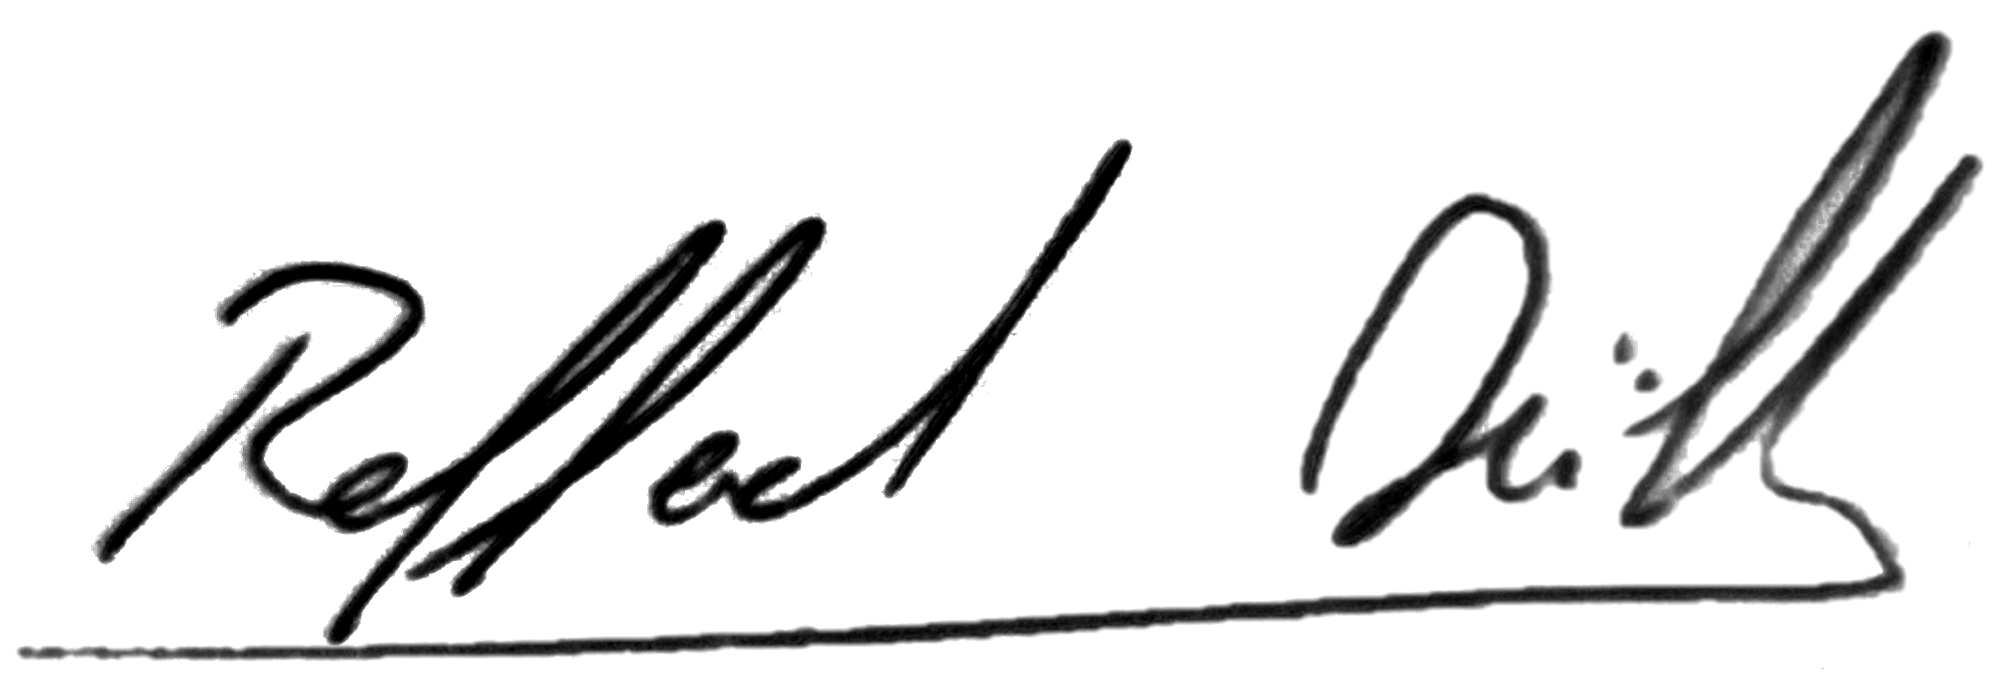
\includegraphics[width=120px,height=40px]{logo/signature_DULL.png}\end{flushright}% signature

    ~\vfill
    \begin{center}
        \begin{minipage}[c]{0.25\linewidth}
            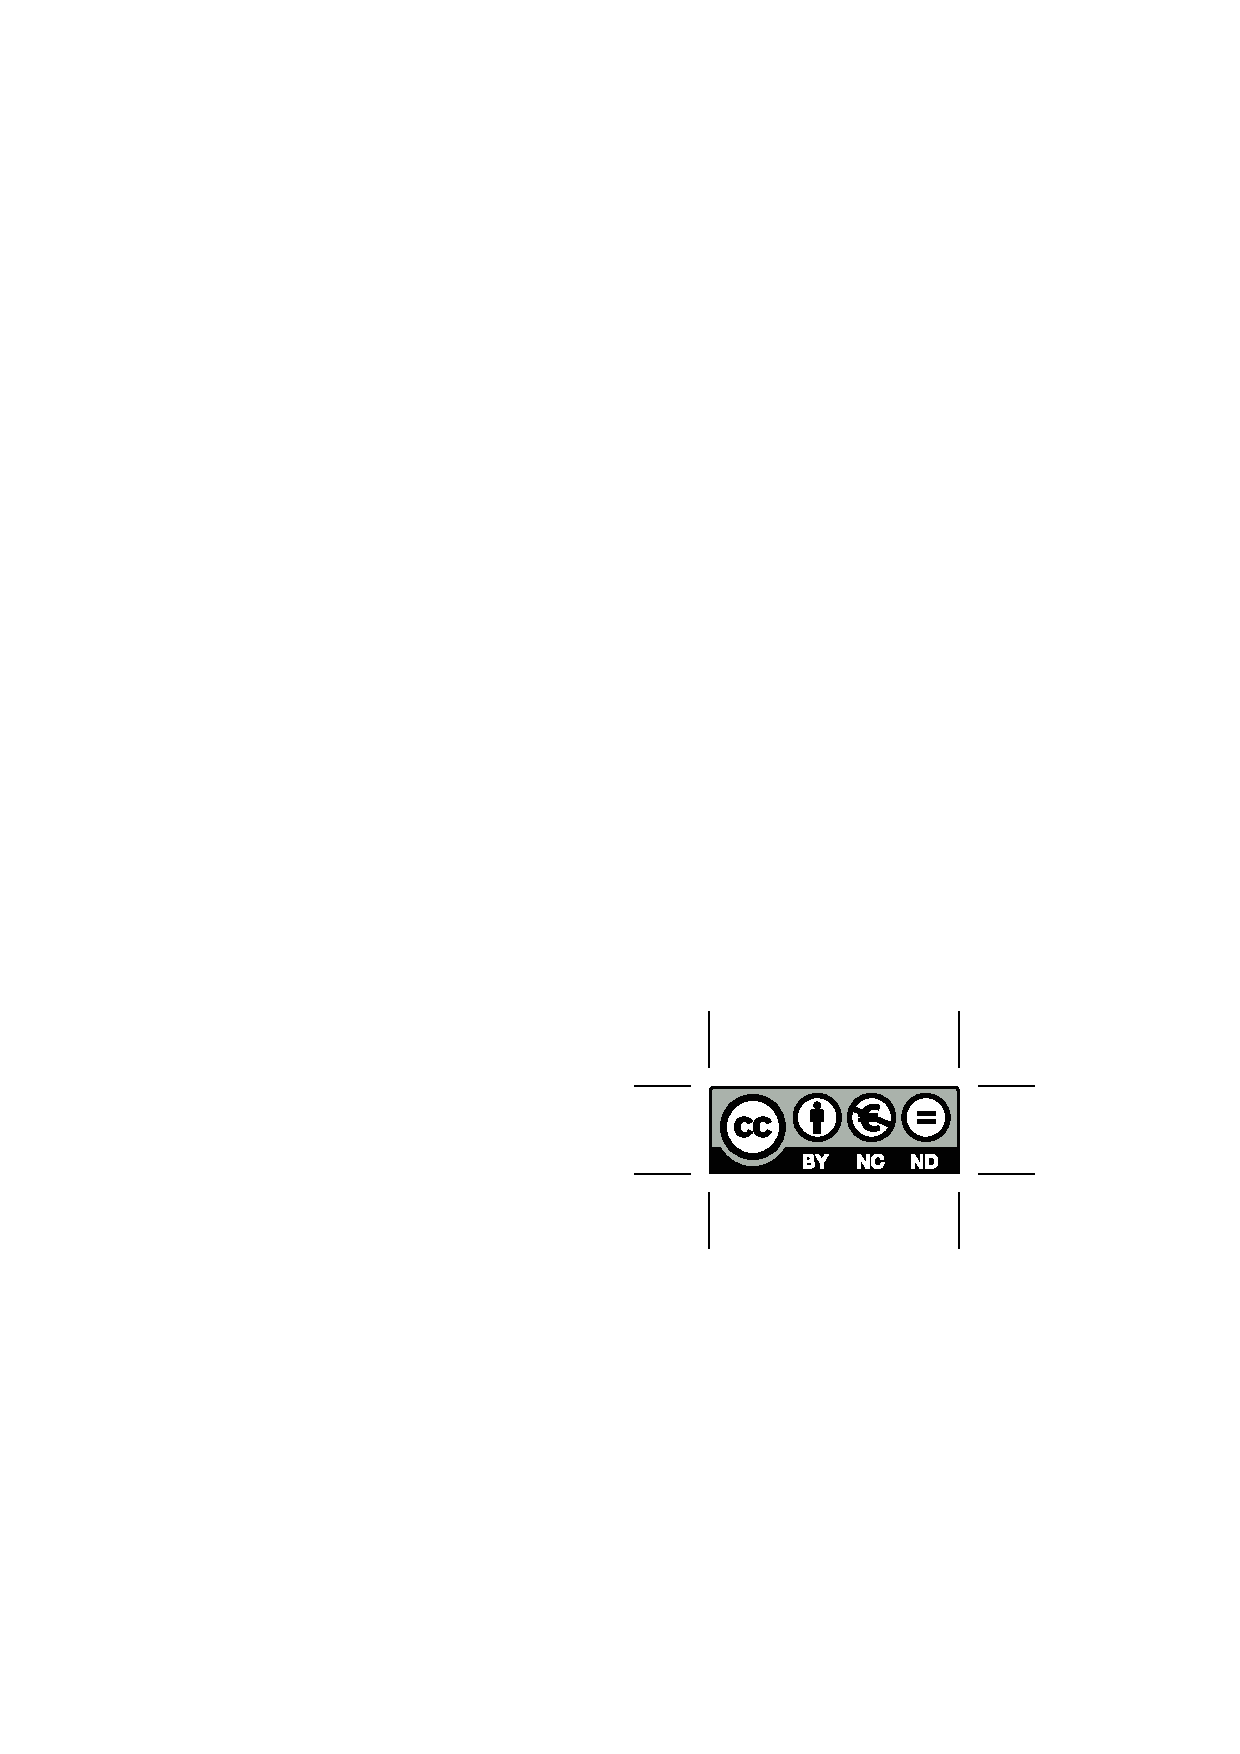
\includegraphics[height=35px]{by-nc-nd-eu}
        \end{minipage}\hfill
    \end{center}

    Cette \oe{}uvre est mise à disposition selon les termes de la \href{https://creativecommons.org/licenses/by-nc-nd/4.0/deed.fr}{Licence Creative Commons Attribution - Pas d’Utilisation Commerciale - Pas de Modification 4.0 International}. % consultez les conditions de la licence cc by-nc-nd, vous pouvez appliquer une licence moins restrictive, cc by-nc-sa par exemple
\fi
\iftrue % Affidavit of Honour for english thesis (invert the \if for an English thesis)
    I, undersigned, Raffael Düll, %% First Name and Surname of the PhD student
    hereby declare that the work presented in this manuscript is my own work, carried out under the scientific supervision of Eric Serre, %% First Name and Surname of the thesis director and if applicable of the co-thesis director
    in accordance with the principles of honesty, integrity and responsibility inherent to the research mission. The research work and the writing of this manuscript have been carried out in compliance with both the french national charter for Research Integrity and AMU charter on the fight against plagiarism.
    
    This work has not been submitted previously either in this country or in another country in the same or in a similar version to any other examination body.\\
    
    Marseille 16/10/2024
    
    \begin{flushright}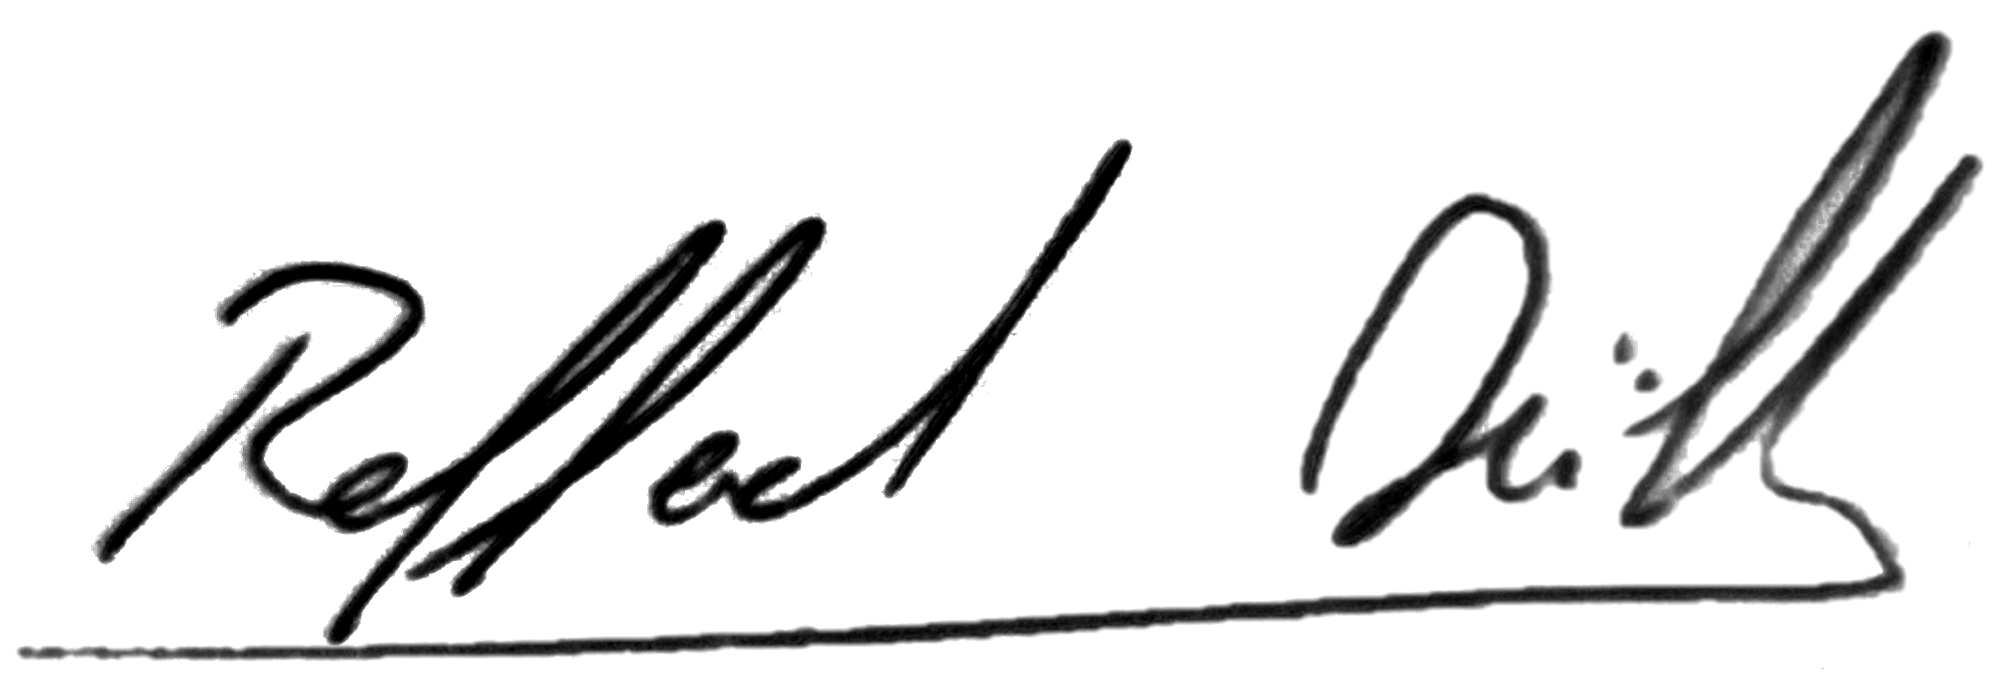
\includegraphics[width=120px,height=40px]{logo/signature_DULL.png}\end{flushright}% signature

    ~\vfill
    \begin{center}
        \begin{minipage}[c]{0.25\linewidth}
            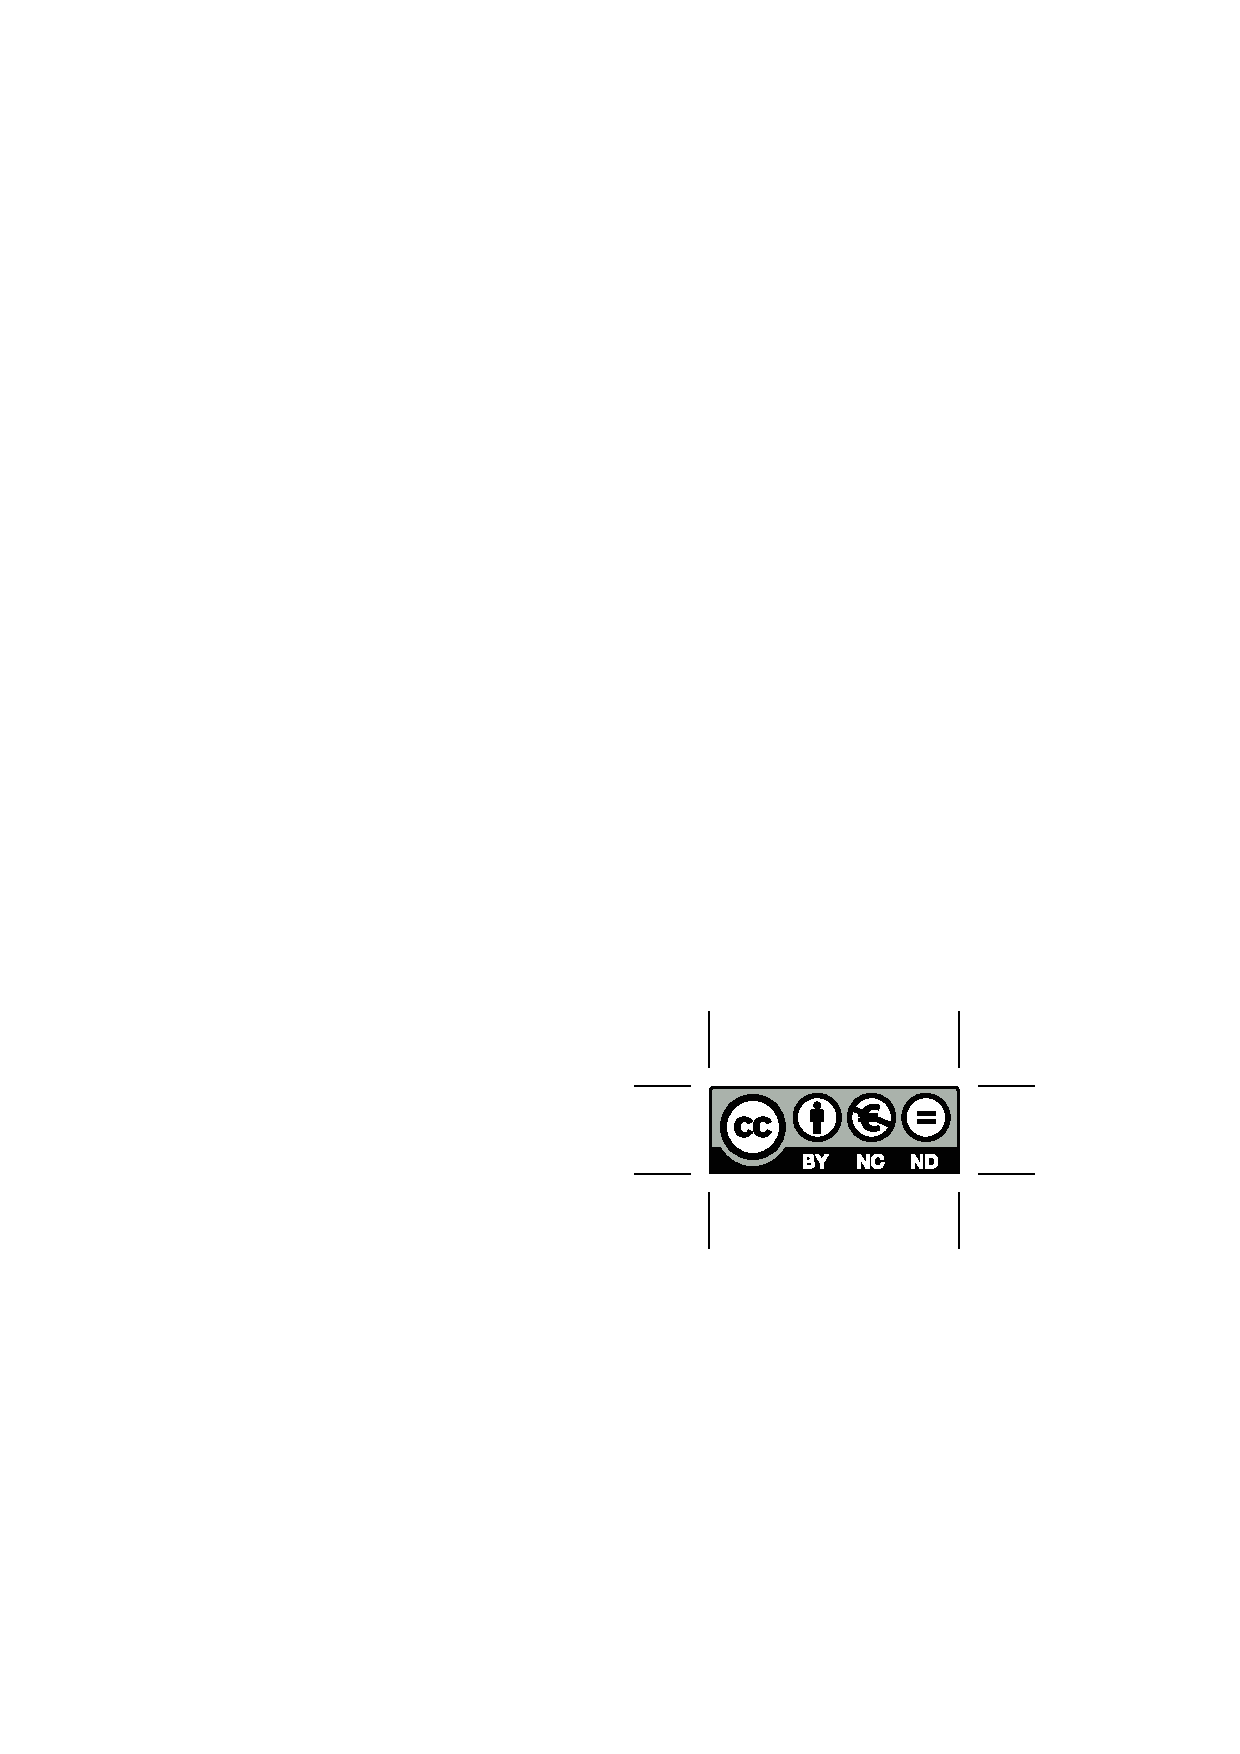
\includegraphics[height=35px]{by-nc-nd-eu}
        \end{minipage}\hfill
    \end{center}

    This work is licensed under \href{https://creativecommons.org/licenses/by-nc-nd/4.0/deed.en}{Creative Commons Attribution-NonCommercial-NoDerivatives 4.0 International Public License}
\fi

				%% affidavit et licence

	\newpage
\addchap{List of publications and/or patents and conference participation}
\label{chap:publications}
\addsec*{(1) List of publications and/or patents produced as part of the thesis project:}
\begin{enumerate}
\item \textbf{Düll, R.}, Bufferand, H., Serre, E., Ciraolo, G., Quadri, V., Rivals, N. and Tamain, P., 2024. Introducing electromagnetic effects in Soledge3X. \textit{Contributions to Plasma Physics}, p.e202300147.
\item \textbf{Düll, R.}, Ciraolo, G. Bufferand, H., Serre, E.,, Quadri, V., Rivals, N., Tamain, P., Sureshkumar, S. and Varadarajan, N. 2024. Implementation of a non-axisymmetric magnetic configuration in SOLEDGE3X to simulate 3D toroidal magnetic ripple effects: Application to WEST. \textit{Nuclear Materials and Energy 41}, p.101807.
\item \textbf{Düll, R.}, Bufferand, H., Serre, E., Ciraolo, G., Quadri, V., Rivals, N., Schwander, F. and Tamain, P., An electromagnetic model in SOLEDGE3X for edge plasma turbulence simulations in tokamak. \textit{Journal of Computational Physics}, preprint available at \url{http://dx.doi.org/10.2139/ssrn.5054729}
\item Bufferand, H., Ciraolo, G., \textbf{Düll, R.}, Falchetto, G., Fedorczak, N., Marandet, Y., Quadri, V., Raghunathan, M., Rivals, N., Schwander, F. and Serre, E., 2024. Global 3D full-scale turbulence simulations of TCV-X21 experiments with SOLEDGE3X. \textit{Nuclear Materials and Energy, 41}, p.101824.
\item De Gianni, L., Ciraolo, G., Giruzzi, G., Falchetto, G., Rivals, N., Balbinot, L., Varadarajan, N., Sureshkumar, S., Artaud, J.F., Bufferand, H. and \textbf{Düll, R.} 2024. Core and edge modeling of JT-60SA H-mode highly radiative scenarios using SOLEDGE3X-EIRENE and METIS codes. \textit{Frontiers in Physics}, 12, p.1422286.
\item Quadri, V., Tamain, P., Marandet, Y., Bufferand, H., Rivals, N., Ciraolo, G., Falchetto, G., \textbf{Düll, R.} and Yang, H., 2024. Self‐organization of plasma edge turbulence in interaction with recycling neutrals. \textit{Contributions to Plasma Physics}, p.e202300146.
\item  Quadri, V., Tamain, P., Marandet, Y., Bufferand, H., Rivals, N., Ciraolo, G., Falchetto, G.L., \textbf{Düll, R.}, Sureshkumar, S., Varadarajan, N. and Yang, H., 2024. Edge plasma turbulence simulations in detached regimes with the SOLEDGE3X code. \textit{Nuclear Materials and Energy}, p.101756.
\item Sureshkumar, S., Rivals, N., Tamain, P., Bonnin, X., Pitts, R., Marandet, Y., Ciraolo, G., Bufferand, H., Falchetto, G., Fedorczak, N., Quadri, V., Raghunathan M., Schwander F., Serre E., \textbf{Düll R.}  and Varadarajan N. 2024. First SOLEDGE3X-EIRENE simulations of the ITER Neon seeded burning plasma boundary up to the first wall. \textit{Nuclear Materials and Energy, 41}, p.101780.
\end{enumerate}


\addsec*{(2) Participation in conferences and summer schools during the thesis period:}
\begin{enumerate}
\item Summer School PlasmaSurf by Instituto de Plasmas e Fus\~{a}o Nuclear. July 2022, Lisbon, Portugal
\item Conference EPS - 49th European Conference on Plasma Physics, European Physical Society. July 2023, Bordeaux, France. Poster presenation: \textit{"A new electromagnetic model in SOLEDGE3X"}
\item Conference PET19 - 19th International Workshop on Plasma Edge Theory in Fusion Devices. September 2023, Hefei, China. Contributed talk: \textit{"Introducing electromagnetic effects in Soledge3X"}
\item Conference PSI-26 - 26th International Conference on Plasma Surface Interaction in Controlled Fusion Devices. May 2024, Marseille, France. Poster presentation: \textit{"Electromagnetic effects on turbulent structures in edge plasmas with SOLEDGE3X"}
\item EUROfusion - TSVV3 Annual Workshop. May 2024, Leuven, Belgium [remote participation]. Presentation: \textit{"Simulating electromagnetic effects in SOLEDGE3X"}
\item Conference ECCOMAS - 9th European Congress on Computational Methods in Applied Sciences and Engineering. June 2024, Lisbon, Portugal. Participation at the mini-symposium: Magnetohydrodinamic Numerical Modeling of Magnetised Plasmas. I with the oral presentation: \textit{"An electromagnetic model for SOLEDGE3X"}
\item EUROfusion - TSVV1 Progress Workshop. September 2024, Garching, Germany. Presentation: \textit{"A new electromagnetic model for turbulent simulations in SOLEDGE3X"}
\end{enumerate}			%% liste de publications et participation aux conférences

	\addchap{Résumé et mots clés}
\label{chap:resume}

\selectlanguage{french}

Dans le bord du tokamak, les gradients abrupts et la courbure magnétique génèrent des structures turbulentes de grande échelle qui transportent les particules de plasma du cœur chaud, où la fusion se produit à environ 10 keV, vers la couche limite (SOL) beaucoup plus froide, où les lignes de champ magnétique croisent la paroi. La turbulence réduit le confinement du plasma et détermine la zone où de forts flux de chaleur impactent le divertor. Le code fluide SOLEDGE3X, développé par le CEA/IRFM en collaboration avec Aix-Marseille Université, s'est avéré efficace pour simuler la turbulence électrostatique résistive des ondes de dérive dans des géométries de tokamak réalistes. Cependant, des résultats expérimentaux et numériques ont montré que les effets électromagnétiques ont un impact significatif sur la dynamique des ondes de dérive, et donc sur la turbulence de bord. \\

Cette thèse introduit un modèle électromagnétique dans SOLEDGE3X, avec trois composantes : l'induction magnétique, le flutter électromagnétique et l'inertie des électrons. L'induction magnétique tient compte de la variation temporelle du potentiel vecteur magnétique parallèle $A_\parallel$ dans la définition du champ électrique parallèle, et $A_\parallel$ est relié à la densité de courant parallèle $j_\parallel$ par la loi d'Ampère. Les fluctuations du champ magnétique, appelées flutter, sont ajoutées au premier ordre et supposées faibles par rapport au champ d'équilibre. L'inertie des électrons, apparaissant avec une masse d'électrons non nulle dans la loi d'Ohm, est nécessaire pour contraindre les vitesses des ondes d'Alfvén à des valeurs physiques. Les nouveaux champs $A_\parallel$ et $j_\parallel$ sont intégrés dans le maillage aligné aux surfaces de flux sur une grille décalée poloïdalement et toroïdalement. Le flutter affecte les équations de transport parallèle et les gradients dans la loi d'Ohm. Sa mise en œuvre a requis une attention particulière pour tenir compte de la nouvelle composante radiale de la direction parallèle $\textbf{b}$. Pour permettre des pas de temps plus importants que les temps d'Alfvén, de transit électronique ou de collision électron-ion, les effets inductifs, inertiels et résistifs sont résolus implicitement dans un système 3D couplé sur les potentiels $\Phi$ et $A_\parallel$. Le modèle a été vérifié au moyen de solutions analytiques et validé sur un cas linéaire, montrant la transition d'ondes d'Alfvén à des ondes électroniques thermiques. \\

Le flutter contribue peu au transport radial, mais influence la réponse non adiabatique du potentiel aux fluctuations de densité. Les premières simulations dans des géométries slab, circulaires (limitées) et à point X (à divertor) montrent de manière consistante que l'inertie des électrons et l'induction magnétique déstabilisent la turbulence des ondes de dérive, tandis que le flutter la stabilise, à la fois dans les phases linéaires et non linéaires. Sur les lignes de champ ouvertes, l'induction magnétique réduit la sensibilité des structures turbulentes aux effets de gaine, favorisant la propagation de la turbulence dans la SOL. Sur le plan numérique, l'inertie des électrons améliore considérablement le conditionnement de la matrice de vorticité, en particulier dans les plasmas chauds à faible résistivité, accélérant la résolution d'un facteur quatre. Cependant, l'ajout du flutter dégrade la performance du code, car il nécessite la résolution de systèmes 3D implicites pour les problèmes de viscosité et de diffusion thermique, auparavant traités comme des systèmes 2D découplés sur chaque surface de flux. Dans le prolongement de ce travail, des perturbations de l'équilibre magnétique ont été imposées de manière externe dans une simulation en mode transport portant sur le dépôt de chaleur dans une configuration magnétique non axisymétrique avec ripple sur WEST.




\vspace{0.5cm}
Mots clés: tokamak, plasma de bord, simulations turbulentes, électromagnétisme, SOLEDGE3X


\selectlanguage{english}										

					%% résumé

	\addchap{Abstract and keywords}
\label{chap:abstract}

In the tokamak edge, steep gradients and magnetic curvature generate large-scale turbulent structures that transport plasma particles from the hot core, where fusion occurs at around 10 keV, to the much colder Scrape-Off-Layer (SOL), where magnetic field lines intersect the physical wall. Turbulence reduces plasma confinement and defines the region where strong heat fluxes impact the divertor. The drift-reduced fluid code SOLEDGE3X, developed by CEA/IRFM in collaboration with Aix-Marseille University, has proven effective in simulating electrostatic resistive drift-wave turbulence in realistic tokamak geometries. However, both experimental and numerical results have shown that electromagnetic effects significantly impact drift-wave dynamics, and thus, edge plasma turbulence. 

This thesis introduces a new electromagnetic model in SOLEDGE3X for the vorticity equation, incorporating magnetic induction, electromagnetic flutter, and electron inertia. Magnetic induction accounts for the time variation of the parallel magnetic vector potential $A_\parallel$ in the definition of the parallel electric field, and $A_\parallel$ is related to the parallel current density $j_\parallel$ via Ampère's law. Fluctuations in the magnetic field, termed flutter, are added at first order and are assumed to be small compared to the equilibrium field. Electron inertia, represented by a finite electron mass in Ohm's law, is necessary to constrain shear Alfvén wave speeds to physical values. The new fields $A_\parallel$ and $j_\parallel$ are integrated into the flux-surface-aligned FVM framework on a poloidally and toroidally staggered grid. Flutter affects the parallel transport equations and gradients in Ohm's law, and its implementation required special care to account for the new radial component of the parallel direction $\textbf{b}$. To handle timesteps larger than Alfvénic, electron thermal, or electron-ion collision times, the corresponding inductive, inertial, and resistive effects are solved implicitly in a coupled 3D system for the potentials $\Phi$ and $A_\parallel$. The model was verified with manufactured solutions and validated on a linear slab case, which demonstrated the expected transition from Alfvén to thermal electron waves as the perpendicular wavenumber increased. 

Flutter contributes minimally to cross-field transport but affects the non-adiabatic potential response to density fluctuations in Ohm's law. Simulations in slab, circular (limited), and X-point (diverted) geometries consistently show that electron inertia and magnetic induction destabilize drift-wave turbulence, while flutter stabilizes it in both the linear and nonlinear phases. On open field lines, magnetic induction reduces the sensitivity of turbulent structures to sheath effects, promoting further turbulence spreading in the SOL. Numerically, electron inertia significantly improves the condition number of the vorticity system, especially in hot plasmas with low resistivity, providing a factor-four speedup even in electrostatic scenarios. However, adding flutter degrades code performance, as it requires solving implicit 3D systems for viscosity and heat diffusion problems that were previously treated as uncoupled 2D systems on each flux surface. As an extension to this work, perturbations to the magnetic equilibrium were externally imposed in a transport mode simulation to study heat deposition in a non-axisymmetric magnetic configuration with ripple on WEST.

\vspace{0.5cm}
Keywords: tokamak, edge plasma, turbulent simulations, electromagnetism, SOLEDGE3X
				%% abstract

	\addchap{Remerciements}
Le modèle de thèse AMU n'existerait pas sans la contribution des doctorants. Nous souhaitons remercier tout particulièrement \href{http://www.theses.fr/2011AIX20720}{Mickaël Bojados}, \href{http://www.theses.fr/2011AIX22111}{Flora Cordoleani} et \href{http://www.theses.fr/2014AIXM4013}{Florian Caullery} pour leur aide précieuse et la qualité de leurs fichiers sources LaTeX. La mise à jour effectuée en 2018 doit beaucoup à l'excellent travail de \href{http://theses.fr/2014ENMP0038}{Dorian Depriester}.

\lipsum[1-2]\index{Nam dui ligula}
				%% remerciements

    \microtypesetup{protrusion=false}	%% désactive la protrusion (TOC LOFT GLS)
	\tableofcontents					%% TOC
	\listoffigures						%% LOF
	\listoftables						%% LOT
	\printglossary[						%% acronymes
		type=\acronymtype,
		title={List of acronymes},
		toctitle={List of acronymes}
		]
	\printglossary[						%% glossaire
		title={Glossary},
		toctitle={Glossary}
		]
	\printglossary[						%% nomenclature
		type=notation,
		title={Naming convention},
		toctitle={Naming convention}
		]
    \microtypesetup{protrusion=true}	%% rétabli la protrusion

	\ohead{\leftmark\Ifstr{\rightmark}{\leftmark}{}{ -- \rightmark}}	%% place le chapître et la partie en en-tête
	h4
	\clearpage
	
	\chapter{Introduction}
\label{chap:Intro}
The sun is the primary source of energy for Earth, and is essential for photosynthesis in plants, which forms the basis of most food chains, and for driving the weather and climate systems that shape our environment. Its consistent radiation supports all life forms, regulates global temperatures, and influences fundamental ecological and biological processes that are vital for the Earth's diverse ecosystems. From the very outset of human life, the sun has been a subject of profound admiration, occupying a central role in various religious beliefs and was often synonym of an incomparably vast and potent source of energy. It was not until the beginning of the twentieth century that progress in particle physics allowed to unravel the secret of solar energy: nuclear fusion. It is the physical process where two light atoms merge to form a heavier atom, releasing significant energy as a result of mass-to-energy conversion. The strong nuclear force is fundamental to confine the positively charged protons with neutrons in an atomic nucleus. Every element is characterized by its total binding energy, that corresponds to the energy needed to break an atom into its constituting protons and neutrons. A higher total binding energy means that the element is more stable. The maximum binding energy is observed for iron ($^{56}Fe$), it means that (roughly) all lighter elements can produce energy by fusion and heavier by fission, as it is done in conventional nuclear power plants.  \newline 

The dream of achieving nuclear fusion in a laboratory to produce energy emerged shortly thereafter. In today's climate crisis, nuclear fusion is even more appealing because it does not emit carbon emissions, does not present the risk of a catastrophic meltdown and its fuel, hydrogen, is readily available. Since replicating the sun's core conditions on Earth, particularly the immense pressure, is not feasible, alternative approaches were searched. A look at Fig. \ref{fig:Intro_fusionCrossSections} with the reaction cross-section of various pairs of light atoms shows that deuterium-tritium (D-T) fusion has the highest likelihood at the most accessible temperature. These two hydrogen isotopes are hence the most favorable candidates for fusion and rhe reaction reads: \newline

\begin{equation}
	^2_1D + ^3_1T \Rightarrow ^4_2He [3.5MeV] \quad + ^1_0n [14.1 MeV]
\end{equation}

In the fusion reaction between deuterium and tritium, one alpha-particle (or Helium-4 nucleus) and one neutron are produced. 80\% of the released energy is carried by the neutron. Deuterium is a naturally abundant isotope of hydrogen, but tritium, which is radioactive and has a relatively short half-life time of 12 years, must be produced artificially. The most widely used method to obtain tritium is via neutron activation of lithium-6, but this requires either a nuclear power plant or another type of effective neutron source. As each fusion reaction emits one neutron, all future D-T reactor designs rely on a yet-to-be-tested technology to produce tritium inside the reactor, in the so-called "tritium breeding" process. To compensate inevitable particle losses, the neutron flux is first multiplied by hitting a layer of beryllium or lead. The neutrons then react with the lithium in an exothermic reaction, releasing one new tritium and one helium atom. The limiting resource for a large-scale deployment of nuclear fusion for power generation is then lithium, but even then, the required quantities are well below the current extraction for industrial needs. \\


\begin{figure}[H]
	\centering
	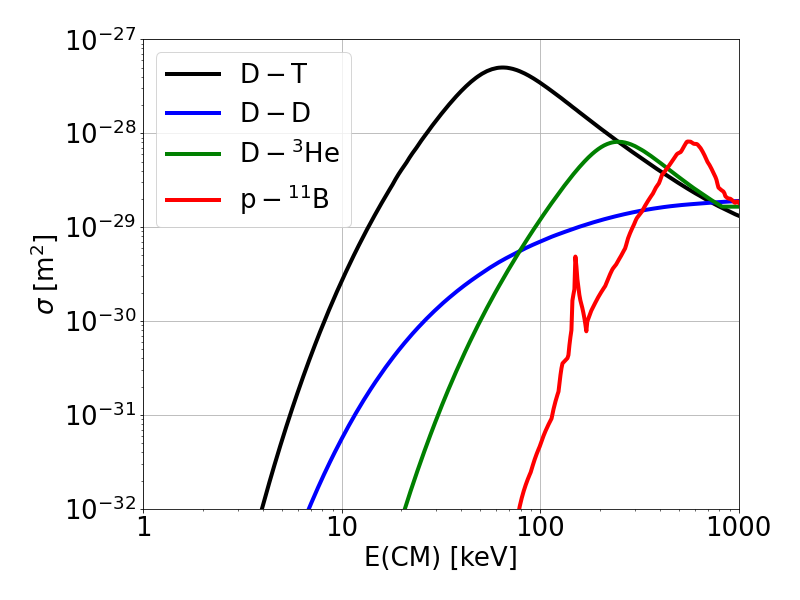
\includegraphics[width=0.62\textwidth]{schemes/fusion-xsecs2.png}
	\caption{Fusion reaction cross-sections for the most promising pairs of light elements over center-of-mass energy.}
	\label{fig:Intro_fusionCrossSections}
\end{figure}


At the very high temperatures needed for nuclear fusion, the electromagnetic force is insufficient to maintain the cohesion of electrons and their atomic nuclei, resulting in the formation of a state of matter known as plasma. Plasma is an ionized gas composed of positively charged nuclei and negatively charged electrons, which interact electromagnetically. \newline

Lawson's criterion \cite{Lawson1957} estimates the necessary plasma conditions to reach the break-even point, where fusion power exceeds heating and conduction losses. For D-T fusion, the triple product of density $n$, temperature $T$, and energy confinement time $\tau_E$ must exceed:

\begin{equation}
	\label{eq:LawsonCriterionDT}
	nT\tau_E > 10^{-21} \, \text{keV} \cdot \text{m}^{-3} \cdot \text{s}
\end{equation}

From a practical point of view, an important metric is the fusion gain $Q$, which measures the ratio of power produced in the nuclear fusion reaction to the required heating power to maintain plasma conditions. One major milestone is the break-even point, when the fusion reaction produces enough power to maintain a steady state at $Q=1$. However, the plasma can only capture a fraction of the produced fusion energy, as most fast neutrons rapidly escape the plasma, with, as seen before, 80\% of the energy. Therefore, external heating is still required until $Q>5$. Past this point, fusion produces more heat than the total required heating power and sustains itself in a state known as ignition ($Q=\infty$). Commercial operation of fusion power plants requires reliable access to ignition, which still requires decades of research. \\

The reaction cross-section determines an optimal temperature of approximately 15-40 keV (~150 million °C) for D-T fusion reactions, leading fusion reactor designs to maximize either of the two remaining parameters: density or confinement time. There is a large variety of approaches to artificial fusion, but today, two concepts show the most promise. Inertial Confinement Fusion (ICF) seeks to compress dense fuel pellets for an extremely brief duration using high-powered lasers. Conversely, Magnetic Confinement Fusion (MCF) utilizes strong magnetic fields to sustain stable plasmas at relatively low densities. Within MCF, there are two primary designs: tokamaks, which use a toroidal chamber with an axisymmetric magnetic field, and stellarators, which use a twisted magnetic configuration to improve plasma confinement.\\

\begin{figure}[H]
	\centering
	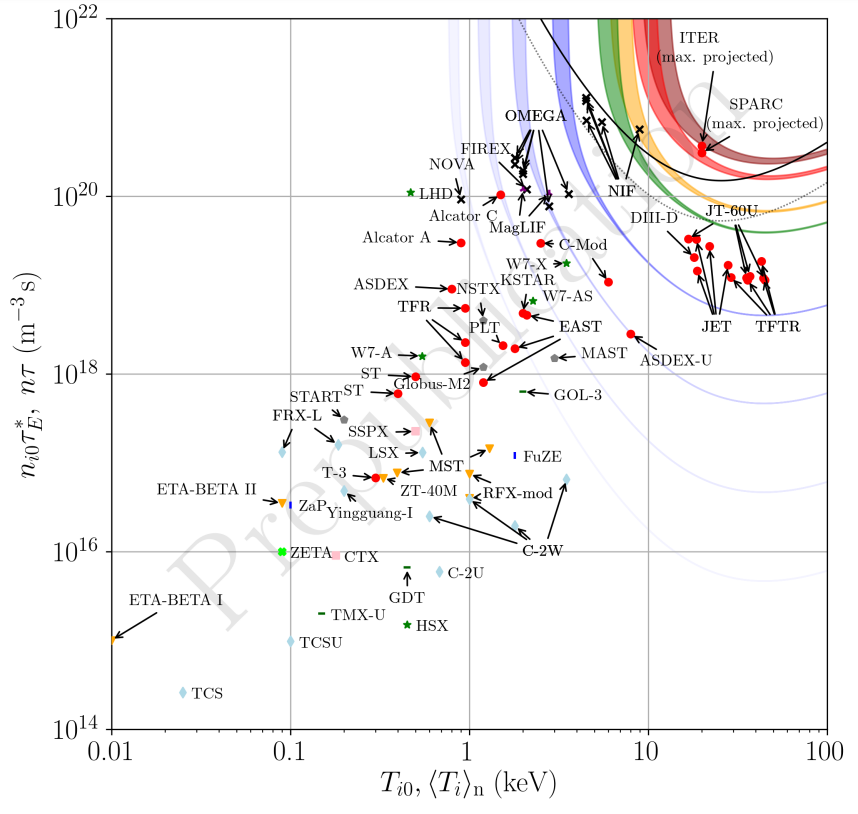
\includegraphics[width=0.7\textwidth]{schemes/Fusion_Triples_2021.png}
	\caption{Relation of the fusion trapping $n\tau_E$ to the temperature in current and future devices. For MCF The break-even point (Q=1) corresponds to the green area and ignition (Q=$\infty$) is brown. Ignition for ICF is reached at the solid black line. Taken from \cite{wurzel2022progress}}
	\label{fig:Intro_fusionTripleProduct}
\end{figure}

Figure \ref{fig:Intro_fusionTripleProduct} depicts the current status of fusion experiments with respect to Lawson's criterion. On December 5, 2022, the National Ignition Facility (NIF) reached the break-even point for the first time, achieving a 3.1 MJ fusion yield with 2 MJ of injected laser power\cite{abu2024achievement}. Large MCF devices, such as DIII-D, TFTR, JET, and JT60-SA, are already very close to the break-even point. Next-generation devices, including ITER and SPARC, which are under construction, are expected to achieve $Q>1$. \\


In this work, we focus on the most promising candidate for MCF, the tokamak. The three Soviet physicists Lavrent'ev, Sakharov, and Tamm had the idea in the early 1950s \cite{azizov2012tokamaks} to confine the plasma in a strong toroidal magnetic field. Additional coils create a poloidal field to suppress instabilities, such that plasma particles are trapped on helical trajectories. The first experiment was conducted in 1954 at the LIPAN institute in Moscow, the predecessor of the Kurchatov institute. The term "tokamak" or "\cyrillic{токамак}" was coined in 1957 by Golovin, and is a Russian acronym of "\cyrillic{тороидальная камера с магнитными катушками}", which translates to "toroidal chamber with magnetic coils," where the "G" from "mag" was transformed to "K" for better sonority \cite{shafranov1999trends}. \\

Since then, tokamaks gained popularity in the USSR and abroad. The design was improved with each generation of new devices to operate at ever higher power. In the 1960s, the first devices surpassed the Bohm limit. Technological progress in plasma heating and superconducting coils led to second-generation tokamaks, such as TFTR and JET, which could operate at much higher temperatures and magnetic field strengths. Another breakthrough was the refined shaping of the magnetic equilibrium with the introduction of divertors to carefully direct particle fluxes, which ultimately culminated in the discovery of the high-confinement (H) mode, allowing for much higher core temperatures. The largest fusion experiment, ITER, is currently under construction in southern France by an international collaboration of seven member parties. At full operation, it is expected to achieve ignition, a state where the fusion reaction emits sufficient radiation to maintain plasma conditions. Its scientific goals include maintaining burning plasma for an extended period of time and demonstrating safe operation in the nuclear phase. It will also serve as a test facility for tritium breeding blankets, a much-needed technology to produce tritium in situ. Currently, tritium is only obtained in pressurized water reactors, and the worldwide annual production of about 500 g is far insufficient to meet the required 55.8 kg per GW installed in a fusion power plant\cite{abdou2020physics}. \\

Understanding fundamental physical processes in the plasma still constitutes an important part of today's research on fusion energy. With the harsh conditions inside the tokamak vessel, diagnostics can only measure indirect plasma properties and are limited in spatial resolution. Simulations are then essential to interpret and extend the findings from experimental data and understand the correlations between different observations. They support current tokamak operation with estimates of heat deposition, wall erosion, and by predicting plasma disruptions. For the design of future fusion devices, simulations allow the evaluation of new magnetic configurations and the optimization of these designs. One particular region of interest is the transition from the hot core region, with closed magnetic field lines, to the edge and the scrape-off layer, where particles traveling along the magnetic field collide with the physical wall in the divertor region. Strong temperature gradients lead to large turbulent structures, driven by resistive drift waves. It is crucial to understand the dynamics and interactions with impurities or neutrals, as fluxes crossing the separatrix largely define the quality of plasma confinement. From a material design perspective, edge plasma simulations are essential to characterize the particle and heat fluxes on the physical wall. \\

The mechanisms at play at the plasma boundary result from the complex interplay of transport processes in the plasma, losses at the wall, and complex atomic and molecular interactions. In this region, particles experience very fast transport along the magnetic field lines and slower, often turbulence-driven, anomalous cross-field transport\cite{loarte2007}. The ratio between these phenomena characterizes the decay length of density and temperature profiles, which further determine the confinement quality of the core plasma and the total heat exhaust on the divertor target. \\

One  major simulation framework that serves this very purpose is the SOLEDGE3X code, originally developed at CEA Cadarache, and extended in the scope of this thesis. Currently, turbulent simulations are limited to L-modes and small machines due to numerical issues and a limited model for larger machines. A significant limitation arises from the anisotropy between the parallel (resistive) and perpendicular (from the time evolution of the vorticity) Laplacians acting on the electric potential. This becomes problematic when the resistivity is very small. Even in the electrostatic collisional regime found in the plasma edge, electron inertia and electromagnetic effects play a substantial role, especially as electron inertia replaces resistivity as it approaches zero. \\

The current implementation of SOLEDGE3X is primarily limited to simulating L-mode plasmas and smaller tokamaks due to various numerical challenges and the limited applicability of its models to larger machines. A significant limitation arises from the anisotropy between the parallel (resistive) and perpendicular (vorticity-driven) Laplacians acting on the electric potential. In the existing electromagnetic model, the vorticity equation is solved implicitly, and as the resistivity approaches zero, the condition number of the matrix deteriorates considerably. Even in the electrostatic, collisional regime typically found in edge plasma, electron inertia and electromagnetic effects play a crucial role, and notably, the finite electron mass in Ohm's law acts as a lower bound for the resistivity. \\

As the plasma approaches the L-H transition, electromagnetic effects become increasingly important. The H-mode is characterized by a suppression of cross-field transport due to "ExB" drifts, which are partially replaced by electromagnetic transport. Significant magnetic reconnection processes lead to important transport of plasma particles from the hot core to the cold edge, with radial fluxes still below "ExB" advection, but non-negligible in understanding the overall plasma behavior. \\

This thesis is dedicated to the implementation of an electromagnetic model within SOLEDGE3X, which includes magnetic induction in the parallel electric field, perturbations of the magnetic equilibrium (flutter), and a finite electron mass in Ohm's law. This development pursues several goals: first, it improves the accuracy of the physical model; second, it enhances numerical robustness by mitigating the poor matrix conditioning associated with low resistivity; and third, it establishes a foundation for self-consistent turbulent simulations that are relevant to larger machines and higher-power scenarios. \\

!!!!!!! PRESENT CHAPTERS OF THE THESIS !!!!!!!!!!


	
	\part[Fundamental Concepts of Fluid Models for Magnetized Plasmas]{Fundamental Concepts of Fluid Models for Magnetized Plasmas}
	\label{part:FundamentalsPlasmaSimulations}
	\chapter{Tokamak Concept}
\label{chap:TokamakConcept}

\vfill
\begin{chaptersummarybox}
	With a given initial velocity, charged particles travel along magnetic field lines on a circular trajectory with the Larmor radius $\rho_L$ and cyclotron frequency $\omega_B$. 
	\begin{align*}
		\rho_L   &= \frac{m\norm{\mathbf{v}_{\perp,0}}}{qB} &
		\omega_B &= \frac{qB}{m}
	\end{align*}	
	Any force perpendicular to the magnetic field causes particles to drift with the velocity $\mathbf{v}_d = \frac{\mathbf{B}\cross\mathbf{F}_\perp}{qB^2}$. To control particle motion, tokamaks employ toroidal and poloidal magnetic fields $B_{\varphi}$ and $B_{p}$ to shape a helical configuration around a torus. To compensate for plasma currents, the magnetohydrodynamic equilibrium causes the so-called Grad-Shafranov shift, which pushes the poloidal field outward. A low ratio between thermodynamic to magnetic pressure, $\beta = \frac{neT}{B^2/2\mu_0}$, is important to avoid plasma instabilities. \\
	At scales beyond the Debye length $\lambda_D = \sqrt{\frac{\varepsilon_0T_e}{n_ee^2}}$, the plasma organizes itself in a state of quasi-neutrality. Collisions between particles cause momentum, energy and charge exchanges, leading to viscosity, heat diffusion and resistivity according to the Spitzer-Härm model:
	\begin{align*}
		\nu_{SH}    &\propto \frac{T_e^{5/2}}{Z^4 \ln \Lambda} &
		\kappa_{SH} &\propto \frac{T_e^{5/2}}{Z \ln \Lambda}   &
		\eta_{SH}   &\propto\frac{Z \ln \Lambda}{T_e^{3/2}}
	\end{align*}
	At the sheath, where magnetic field lines intersect the tokamak wall, a net negative charge develops that attracts ions at high speeds. In divertors, the heat exhaust is concentrated on two thin target lines, and the width $\lambda_q$ is critical for reactor designs.
\end{chaptersummarybox}
\vfill

\newpage

Fusion reactions require extreme temperatures at about 15keV to happen. At such high temperatures, any matter transforms into an ionized state, called plasma, where electrons are dissociated from their atomic core. Charged particles are particularly responsive to magnetic fields, a property that will be used by tokamaks to confine the hot plasma and protect the physical walls of the device. 

A deuterium plasma is an ionized gas comprising positively charged ions ($D^+$) and negatively charged electrons ($e^-$). Initially, both species exhibit independent dynamics. Despite having exactly opposite charges, ions are significantly heavier than electrons, with a mass ratio of $m_i/m_e \approx 3.7\cdot 10^3$. Both ions and electrons can be described by their respective momenta and temperatures. In Sec. \ref{sec:intro_particlesInPlasma}, we first describe their independent behavior in a magnetized environment, then how species interact in Sec. \ref{sec:intro_particlesInteration} and we finish with Sec. \ref{sec:intro_SOL} about the importance of the Scrape-Off-Layer.


\section{Particles in a magnetized plasma}
\label{sec:intro_particlesInPlasma}

This first section describes the fundamental working principle of plasma confined in a tokamaks. Before all, we must understand how charged particles behave when exposed to strong magnetic fields (in Sec. \ref{ssec:intro_magneticConfinement}) and how they experience drifts in perpendicular direction (in Sec. \ref{ssec:intro_plasmaDrifts}). This knowledge allows us to design a magnetic "cage", in which particles are trapped, or confined (in Sec. \ref{ssec:intro_tokamakConfiguration}). The governing equations of this magnetic configuration are given in Sec. \ref{sec:intro_GradShafranov} and Sec. \ref{ssec:intro_limitedDivertedConfig} introduces and compares limited and diverted configurations.

\subsection{Gyromotion of a single particle}
\label{ssec:intro_magneticConfinement}
To understand how charged plasma particles can be confined on a magnetic field line, we consider the simplest example of a single particle with charge \( q \) in a homogeneous, unidirectional magnetic field \(\textbf{B}\) with directional unit vector \(\textbf{b}\). The amplitude of the magnetic field is then $B$ such that $\mathbf{B} = B\mathbf{b}$. Solely the magnetic component of Lorentz's force acts on a particle with mass \( m \) and charge \( q \), leading to the following equation for its velocity \(\textbf{v}\):

\begin{equation}
	\label{eq:gyromotion_LorentzForce}
	m\dv{\textbf{v}}{t} = q\textbf{v}\cross\textbf{B}
\end{equation}

To solve this differential equation, it is convenient to decompose the velocity vector into a parallel component \( v_\parallel = \textbf{v}\cdot\textbf{b} \) and a perpendicular component \( \textbf{v}_\perp = \textbf{v} - v_\parallel \textbf{b} \). For a given initial velocity \(\mathbf{v}_0\), the general solution of this system is:

\begin{equation}
	\mathbf{v}(t) = v_{\parallel,0}\mathbf{b} + \mathbf{v}_{\perp,0}\cos(\omega_B t) + \mathbf{b} \times \mathbf{v}_{\perp,0} \sin(\omega_B t)
\end{equation}

with \(\omega_B = \frac{qB}{m}\) being the cyclotron frequency. This implies that a charged particle circles around a magnetic field line while following it with its initial velocity. The opposite charges of ions and electrons result in them circling in different directions. The trajectory is qualitatively shown in Fig. \ref{fig:TokamakBasics_gyromotion}. The radius of this gyromotion is called the Larmor radius \(\rho_L\):

\begin{equation}
	\rho_L = \frac{m\norm{\mathbf{v}_{\perp,0}}}{qB}
\end{equation}

Because of the high mass ratio, ions have a much larger Larmor radius than electrons. This gyromotion is the fundamental mechanism behind magnetic confinement. \newline 


\begin{figure}[H]
	\centering
	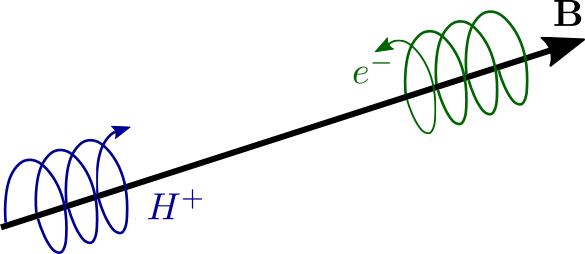
\includegraphics[width=0.62\textwidth]{schemes/gyromotion.png}
	\caption{Trajectory of a positively and a negatively charged particle along a homogeneous magnetic field line.}
	\label{fig:TokamakBasics_gyromotion}
\end{figure}


For a non-homogeneous field, Eq. \ref{eq:gyromotion_LorentzForce} does not necessarily have a straightforward solution. To assume gyromotion as the fundamental dynamic for particles, the magnetic field must remain relatively constant along the helical path traced by the field lines. This requirement imposes a criterion on the Larmor radius, known as adiabatic theory:
\begin{equation}
	\label{eq:intro_adiabaticCondition}
	\rho_L \ll \frac{B}{\norm{\grad B}}
\end{equation}


\subsection{Plasma drifts}
\label{ssec:intro_plasmaDrifts}

Plasma drifts refer to the movement of charged particles under the influence of electric and magnetic fields. These drifts do not account for the primary motion along the guiding center, as described in Section \ref{ssec:intro_magneticConfinement}. To study drift velocities, it is convenient to decompose every vector quantity into an average parallel component and a fluctuating perpendicular component, such that $\mathbf{X} = X_\parallel\mathbf{b} + \mathbf{X_\perp}$. We then express the Lorentz force equation as:

\begin{equation}
	\label{eq:edge_LorentzEquationDecomposition}
	m\partial_t\left(v_\parallel\mathbf{b} + \mathbf{v}_\perp\right) = q\left[E_\parallel\mathbf{b} + \mathbf{E}_\perp + \left(v_\parallel\mathbf{b} + \mathbf{v}_\perp\right) \times \mathbf{B}\right]
\end{equation}

Focusing on the particle's acceleration in the perpendicular direction, we derive the equation of motion:

\begin{equation}
	\label{eq:edge_EcrossBdrift}
	m\partial_t \mathbf{v}_\perp = q\left[\mathbf{E} + \left(\mathbf{v}_\perp \times \mathbf{B}\right)\right]
\end{equation}

In steady-state conditions, the electric force compensates the Lorentz force, leading to the electric drift $\mathbf{v}_E$, commonly referred to as the "E cross B" or simply "ExB" drift:

\begin{equation}
	\mathbf{v}_E = \frac{\mathbf{E}_\perp \times \mathbf{B}}{B^2}
\end{equation}

This velocity applies uniformly to all particles at all times, as it depends only on the electric and magnetic fields in place. Since neither the mass nor the charge contributes to $\mathbf{v}_E$, both electrons and ions move in the same direction at the same speed, and under the quasi-neutrality assumption, no current is generated.

For the next drift, we consider the gyromotion of a particle in a non-uniform magnetic field. Under the adiabatic condition from Eq. \ref{eq:intro_adiabaticCondition}, the magnetic moment $\mu$ of the gyrating particle is conserved along its trajectory:

\begin{equation}
	\mu = \frac{m\norm{\mathbf{v}_\perp}^2}{2B}
\end{equation}

This moment leads to a potential $U = -\mu B$, which exerts a force on the particle:

\begin{equation}
	F_{\nabla B} = -\nabla U = \frac{mv_\perp^2}{2B}\nabla B
\end{equation}

This force acts in the direction of the gradient $\nabla B$, where the magnetic field strength is lower, allowing the particle to reduce its potential energy. This results in the "grad B" drift:

\begin{equation}
	\mathbf{v}_{\nabla B} = \frac{mv_\perp^2}{2q} \frac{\mathbf{B} \times \nabla B}{B^3}
\end{equation}

The helical configuration of a tokamak causes magnetic field lines to bend. To follow the direction of $\mathbf{B}$, the particle's trajectory is curved, and a centripetal force is exerted on the particle. With the curvature radius $\mathbf{R}_c = \mathbf{b} \cdot \nabla \mathbf{b}$, the force is given by:

\begin{equation}
	\mathbf{F}_c = \frac{mv_\parallel^2}{R_c}\mathbf{R}_c = -mv_\parallel^2\frac{\mathbf{B} \cdot \nabla \mathbf{B}}{B^2}
\end{equation}

This force induces the "curvature" drift $\mathbf{v}_c$:

\begin{equation}
	\mathbf{v}_c = \frac{mv_\parallel^2}{q}\frac{\mathbf{B} \times (\mathbf{B} \cdot \nabla \mathbf{B})}{B^4}
\end{equation}

The polarization drift occurs if the electric field in the plasma varies with time. 

\begin{equation}
	\mathbf{v}_p = \frac{m}{qB^2}\frac{d\mathbf{E}}{dt}
\end{equation}

Note that the directions of "grad B", curvature or polarization drifts depend on the particle's charge, causing electrons and ions to move in opposite directions and generating an effective current. The total perpendicular velocity acting on a confined particle is the sum of all these drifts:

\begin{equation}
	\mathbf{v}_d = \mathbf{v}_E + \mathbf{v}_{\nabla B} + \mathbf{v}_c + \mathbf{v}_p
\end{equation}

In fact, any force perpendicular to the magnetic field will cause a drift:

\begin{equation}
	\mathbf{v}_F = \frac{\mathbf{B}\cross\mathbf{F}_\perp}{qB^2}
\end{equation}

All other eventual forces, such as magnetic or gravitational forces, play a subordinate role in the plasma edge and are usually not considered in fluid models. Drift velocities are always orientated in perpendicular direction to then magnetic fields. They do not interfere with (the averaged) parallel fluxes, at a magnitude of $v_{th}$, and are primarily responsible for cross-field fluxes.





\subsection{Tokamak configuration}
\label{ssec:intro_tokamakConfiguration}
Maxwell's law stipulates that the magnetic field must be divergence-free, \(\grad\cdot\mathbf{B} = 0\). Since constructing an infinitely long machine is impractical, particle confinement requires that a given field line be closed, meaning that following its path would return one to the initial position. This necessitates some bending of the magnetic field lines. \newline
The fundamental principle of a tokamak lies in its magnetic configuration, which is designed to confine hot plasma within a toroidal chamber. This configuration comprises two primary magnetic field components: the toroidal field \( B_\varphi \) and the poloidal field \( B_p \). Coils encircling the torus generate the toroidal field, which runs parallel to the circular path of the tokamak and serves to confine the plasma. A strong current passing through the plasma itself induces the poloidal field. The combination of these fields creates a twisted, helical magnetic field structure, as shown in Fig. \ref{fig:1_magneticConfigurationTorus}, that stabilizes the plasma and helps maintain its shape and position within the tokamak.


\begin{figure}[H]
	\centering
	\begin{subfigure}[b]{0.4\textwidth}
		\centering
		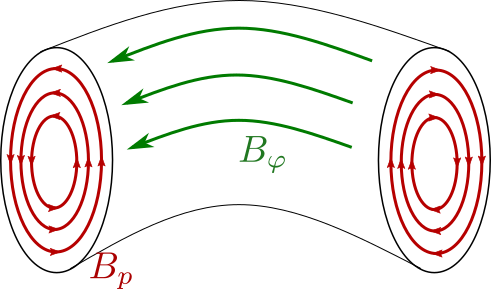
\includegraphics[width=1.\textwidth]{schemes/BpolBtor.png}
		\subcaption{Poloidal and toroidal fields}
		\label{fig:TokamakBasics_BpolBtor}
	\end{subfigure}
	\begin{subfigure}[b]{0.4\textwidth}
		\centering
		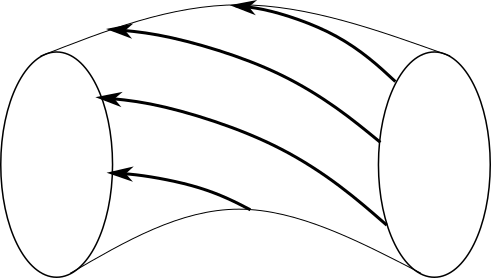
\includegraphics[width=1.\textwidth]{schemes/Btot.png}
		\subcaption{Resulting helical magnetic field}
		\label{fig:TokamakBasics_Btot}
	\end{subfigure}
	\caption{Simplified scheme of the magnetic field components on a flux surface (a) and the total magnetic field (b).}
	\label{fig:1_magneticConfigurationTorus}
\end{figure}

The helical configuration of a magnetic field line in a tokamak ensures that tracing its path remains within the same toroidal surface, ultimately returning to the initial point and forming a closed field line. The ensemble of all such field lines constitutes what is termed a "closed magnetic flux surface." These flux surfaces are radially concentric, and the principle of magnetic confinement is to trap plasma particles within these flux surfaces.  \\

At first glance, the toroidal field appears sufficient to close magnetic field lines. However, plasma drifts inevitably add a dynamic perpendicular to the motion parallel to the magnetic field. Internal and external perturbations can cause twisting of the magnetic field lines, potentially leading to disruptions and total loss of plasma confinement. This phenomenon is known as kink instabilities. To suppress them, the poloidal field introduces magnetic shear to the configuration, with field lines circling around the minor radius of the torus. The ratio of toroidal to poloidal rotations of the field lines is known as the safety factor \( q = \frac{aB_\varphi}{RB_p} \). In a cylindrical approximation, the Kruskal-Shafranov limit \cite{shafranov1956stability, kruskal1958instability} states that kink instabilities are suppressed for \( q > 1 \). However, the safety factor cannot be too large either, as other instabilities such as tearing \cite{furth1973tearing} or resistive wall \cite{fitzpatrick2002simple} modes might appear and deteriorate plasma confinement. \\



\subsection{Grad-Shafranov equilibrium}
\label{sec:intro_GradShafranov}

How can the magnetic configuration be described in a more mathematical way? The magnetic configuration of a tokamak can be described mathematically in cylindrical coordinates \( (R,Z,\varphi) \) with the corresponding basis vectors \([\mathbf{e}_R,\mathbf{e}_Z,\mathbf{e}_\varphi]\). The magnetic field consists of two main components: the poloidal field \(\mathbf{B}_p\), which lies in the \((R,Z)\) plane (referred to as the "poloidal plane"), and the toroidal field \(\mathbf{B}_\varphi\), which is aligned along the \(\varphi\)-direction.

Each magnetic field \(\mathbf{B}\) is associated with a vector potential \(\mathbf{A}\) such that:

\begin{equation}
	\label{eq:intro_magneticVectorPotential}
	\nabla \times \mathbf{A} = \mathbf{B}
\end{equation}

Assuming axisymmetry, gradients along the \(\varphi\)-direction vanish. Let \(\mathbf{A} = A_R \mathbf{e}_R + A_Z \mathbf{e}_Z + A_\varphi \mathbf{e}_\varphi\) represent the three components of the vector potential. The magnetic field can then be expressed as:

\begin{equation}
	\mathbf{B} = \left(\frac{1}{R}\pdv{(RA_\varphi)}{Z}\right)\mathbf{e}_R - \left(\frac{1}{R}\pdv{(RA_\varphi)}{R}\right)\mathbf{e}_Z + \left(\pdv{A_Z}{R} - \pdv{A_R}{Z}\right)\mathbf{e}_\varphi
\end{equation}

Introducing the poloidal flux function \(\Psi = -RA_\varphi\), which shapes \(\mathbf{B}_p\), and the toroidal field function \(F = RB_\varphi\), the magnetic field components can be written as:

\begin{equation}
	\label{eq:intro_BeqMagneticFluxes}
	\mathbf{B} = \underbrace{\nabla \Psi \times \nabla \varphi}_{\mathbf{B}_p} + \underbrace{F \nabla \varphi}_{\mathbf{B}_\varphi}
\end{equation}

In a tokamak, the plasma is not uniform, leading to a pressure gradient from the colder edge to the hotter core. In a stationary plasma that has reached magnetohydrodynamic (MHD) equilibrium, the magnetic and pressure forces must balance, which is described by the force balance equation:

\begin{equation}
	\nabla p = \mathbf{j} \times \mathbf{B}
\end{equation}

Because of the cross-product, $\nabla p$ is always perpendicular to $\mathbf{B}$, implying that $p$ must be constant along a field line. Under the assumption of axisymmetry, $\partial_\varphi p = 0$, meaning that the toroidal component of the magnetic force must be zero. Consequently, only the poloidal field $\mathbf{B}_p$ responds to a pressure gradient. Since the pressure $p(\Psi)$ is both axisymmetric and field-aligned, it can only be a function of the poloidal flux $\Psi$. The toroidal component of the current density can be expressed as:

\begin{equation}
	j_\varphi = R\frac{dp}{d\Psi} + \frac{F}{\mu_0 R}\frac{dF}{d\Psi}
\end{equation}

Ampère's law relates the current density $\mathbf{j}$ to the magnetic field $\mathbf{B}$, with the vacuum permeability $\mu_0$:

\begin{equation}
	\mu_0\mathbf{j} = \nabla \times \mathbf{B}
\end{equation}

This gives an alternative expression for the toroidal current:

\begin{equation}
	j_\varphi = \frac{1}{\mu_0}\left[\partial_R\left(\frac{1}{R}\partial_R\Psi\right) + \frac{1}{R}\partial_Z^2\Psi\right]
\end{equation}

By equating both expressions for $j_\varphi$, we arrive at the Grad-Shafranov equation\cite{grad1958hydromagnetic,shafranov1957equilibrium} for the poloidal flux:

\begin{equation}
	\label{eq:intro_GradShafranovEquation}
	\Delta^* \Psi = R\partial_R\left(\frac{1}{R}\partial_R\Psi\right) + \partial_Z^2\Psi = -\mu_0R^2\frac{dp}{d\Psi} - \mu_0 F \frac{dF}{d\Psi}
\end{equation}
Here we introduced the Shafranov operator $\Delta^*$.
This equation is a second-order nonlinear partial differential equation. The procedure outlined in Appendix \ref{sec:app_GradShafranovSolver} solves Eq. \ref{eq:intro_GradShafranovEquation} iteratively using a Newton-Krylov method. A typical solution for $\Psi$ is illustrated in Fig. \ref{fig:1_PsiFlux}.

\begin{figure}[H]
	\centering
	\begin{subfigure}[b]{0.45\textwidth}
		\centering
		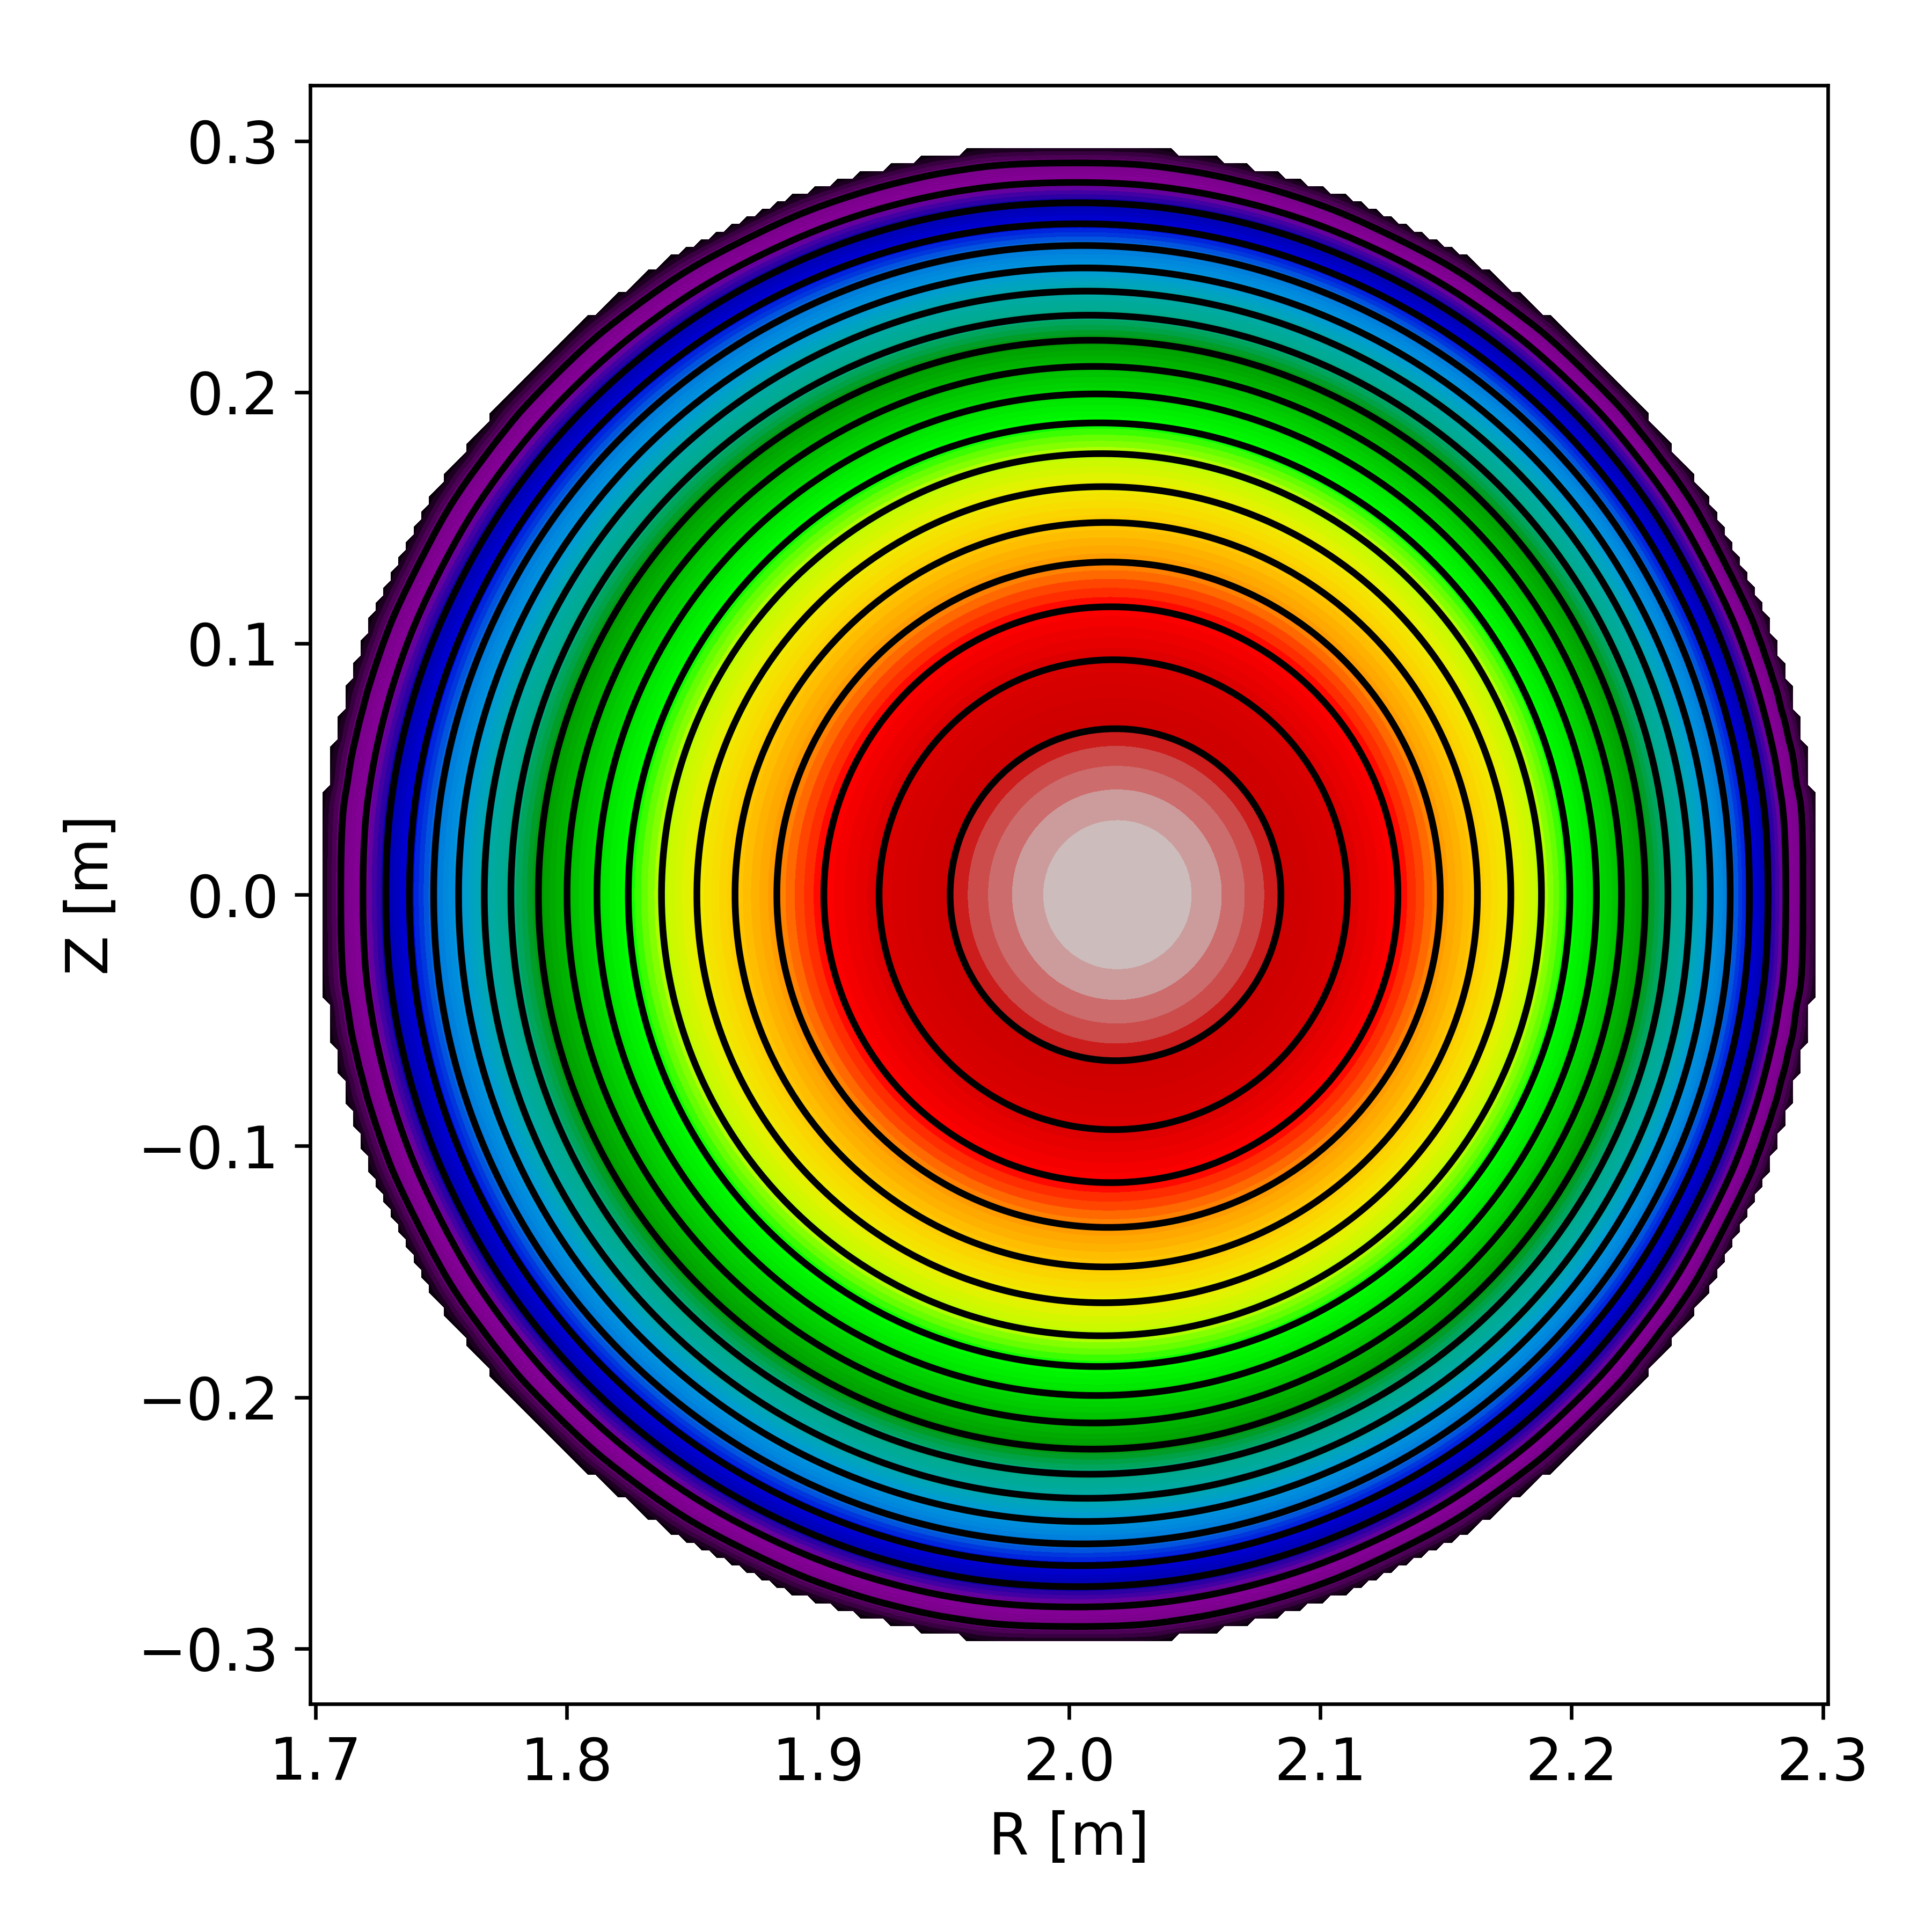
\includegraphics[height=60mm]{schemes/Psi_GradShafranov_R_2.png}
		\subcaption{Major radius $R_0 = 2$m}
		\label{fig:GS_PSI_R_2}
	\end{subfigure}
	\begin{subfigure}[b]{0.45\textwidth}
		\centering
		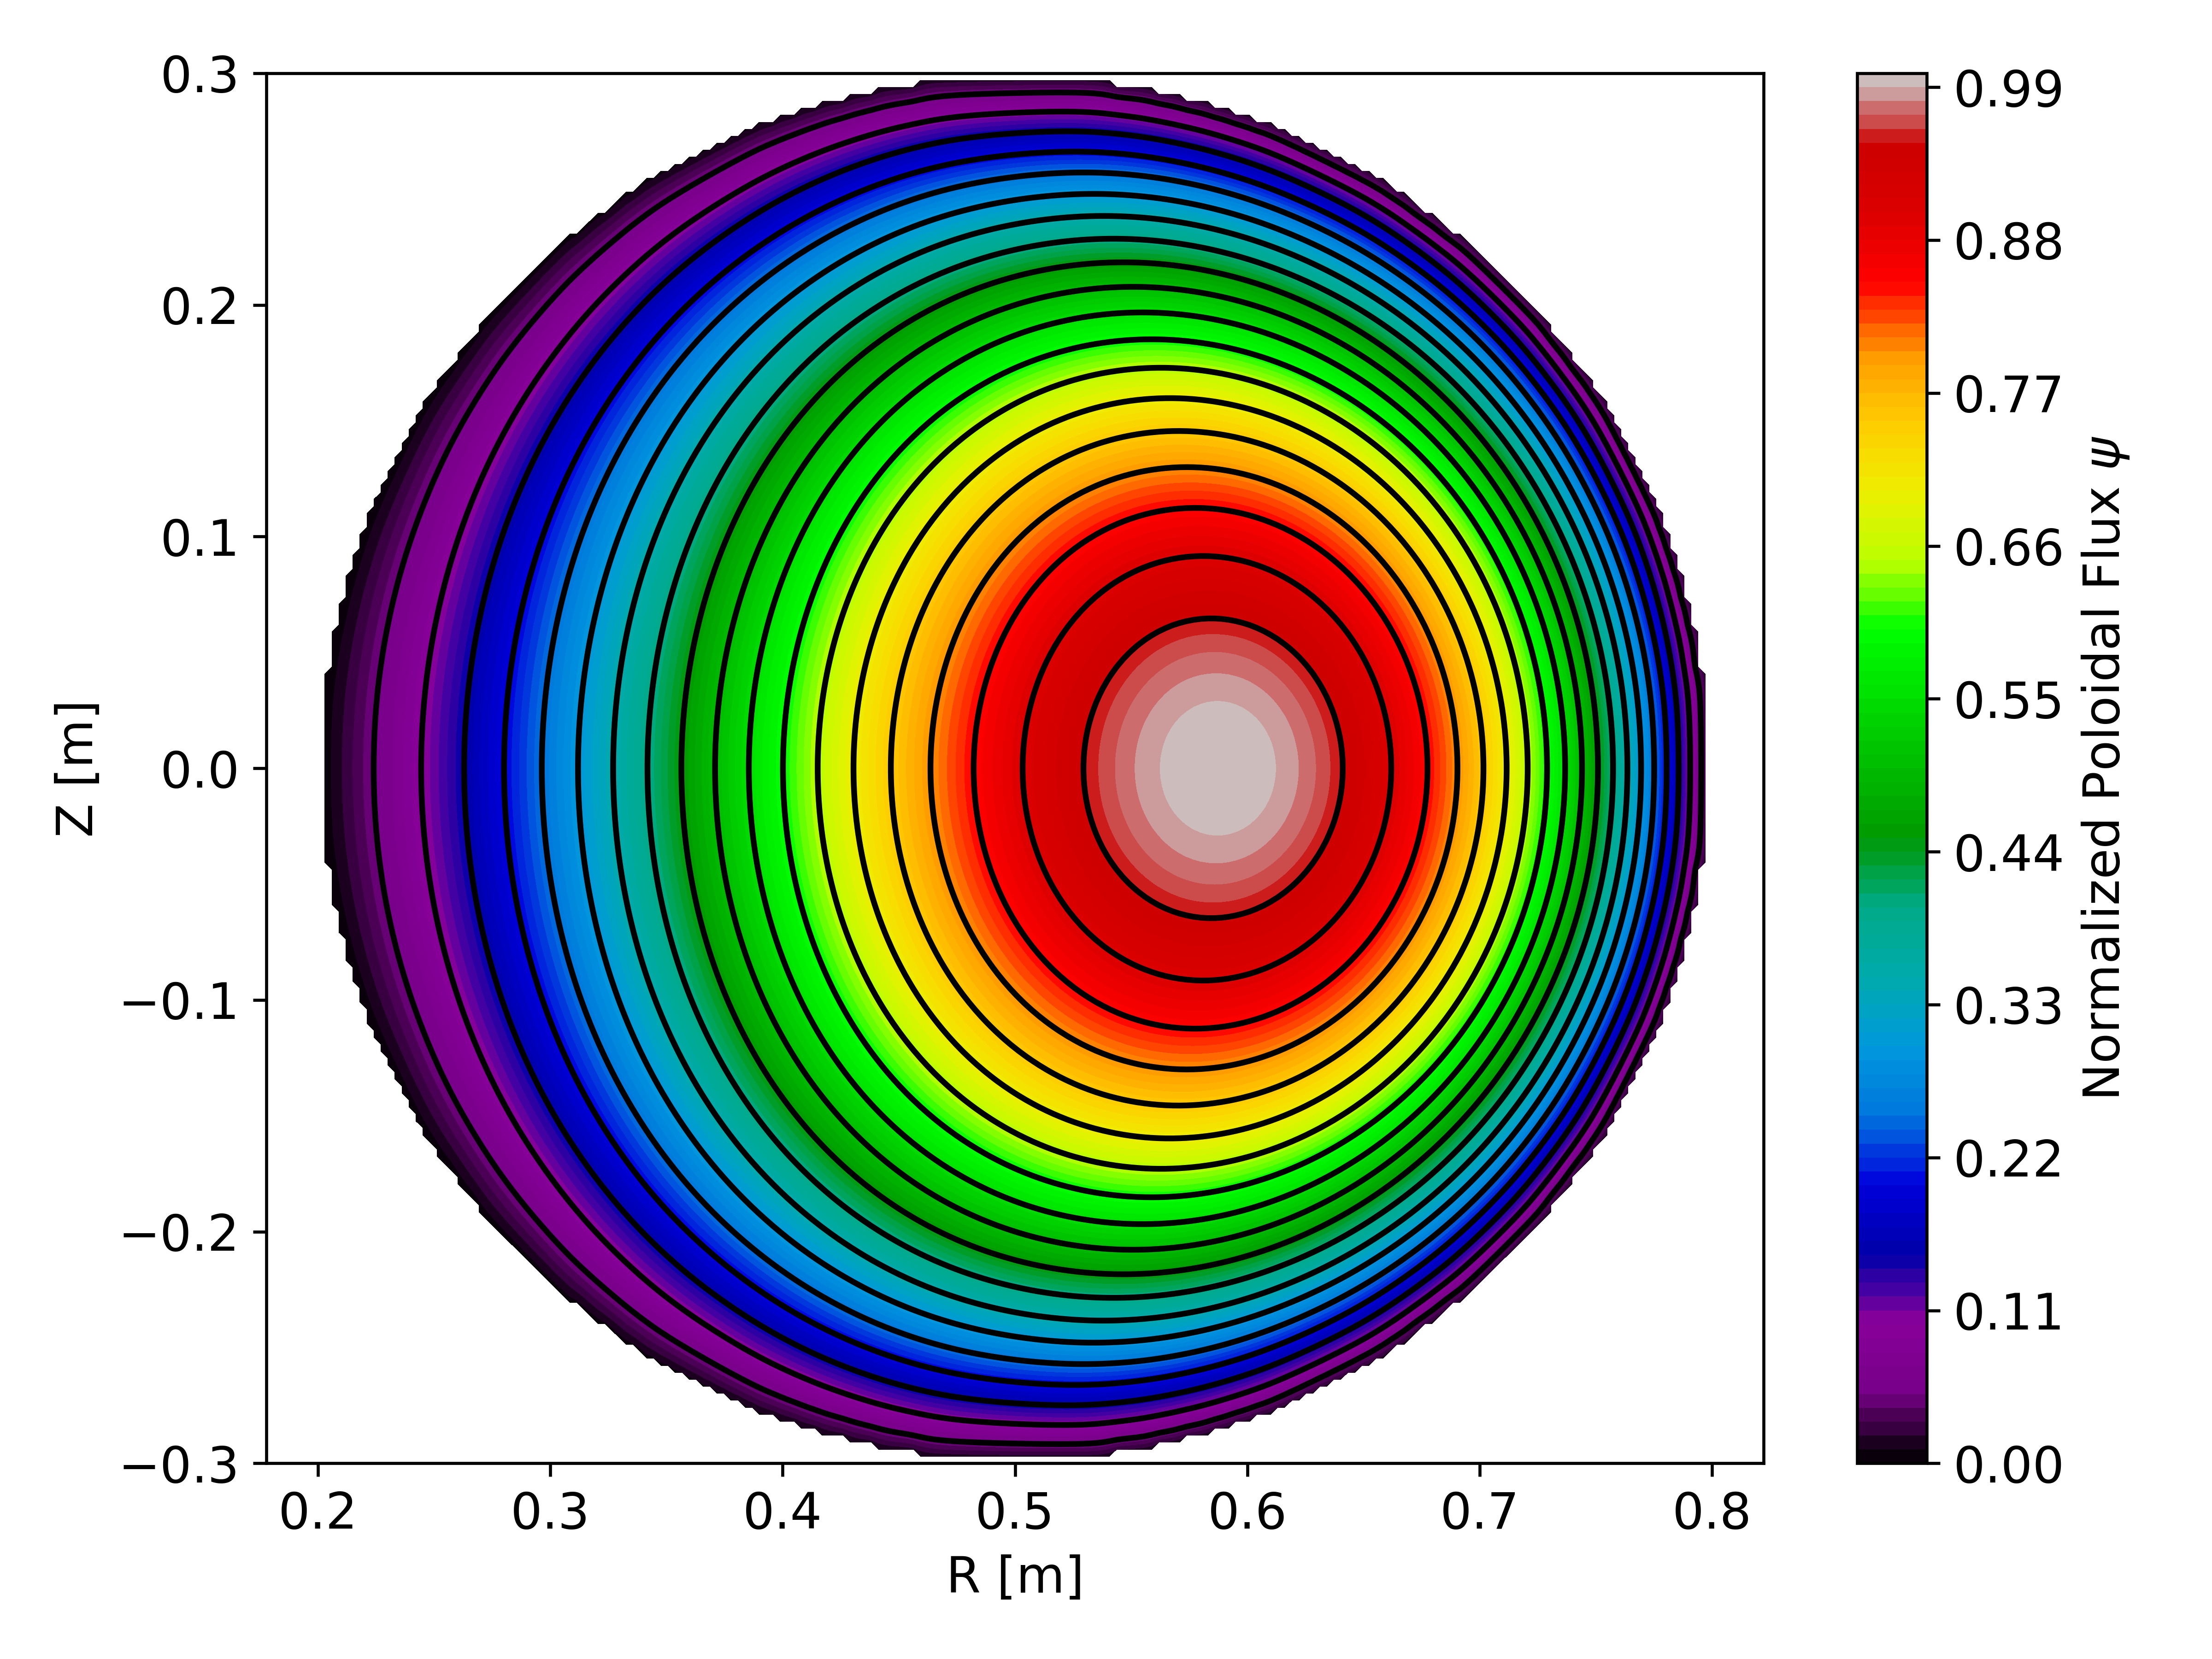
\includegraphics[height=60mm]{schemes/Psi_GradShafranov_R_0_5.png}
		\subcaption{Major radius $R_0 = 0.5$m}
		\label{fig:GS_PSI_R_0_5}
	\end{subfigure}
	\caption{Solution of the Grad-Shafranov equation on a circular cross-section with minor radius $a = 0.3$ m. A Cartesian mesh with $N = 200$ equidistant discretization points is used for the $R$ and $Z$ coordinates. The flux $\Psi$ is forced to 0 at the boundary. The toroidal magnetic field is given by $B_\varphi = B_0 R_0 / R$ with $B_0 = 1$T. The pressure follows an exponential distribution $p(\Psi) = p_0 (e^{-\Psi} - 1)$ with $p_0 = 1$ MPa.}
	\label{fig:1_PsiFlux}
\end{figure}

The plasma pressure causes the magnetic axis to shift outward in a phenomenon known as the Grad-Shafranov shift. The radial displacement from the centerline of the torus can be approximated by:

\begin{equation}
	\label{eq:intro_GradShafranovShift}
	\Delta \approx \frac{2\mu_0 p}{B_p}\frac{a^2}{R_0}
\end{equation}

The two scenarios presented in Fig. \ref{fig:1_PsiFlux} differ by their major radius. As the Grad-Shafranov shift is inversely proportional to $R_0$, we expect that the larger curvature in the case \ref{fig:GS_PSI_R_0_5} $R_0 = 0.5$m induces a larger shift, which is precisely what is observed. \\

An important metric in this context is the ratio $\beta$ of plasma pressure over magnetic pressure.

\begin{equation}
	\label{eq:PlasmaBeta}
	\beta = \frac{p}{p_{mag}} = \frac{neT}{B^2/2\mu_0}
\end{equation}

There is a concurrent dynamic between thermodynamic and magnetic pressures: the former exerts an expansive force on the plasma, while the latter seeks to confine the plasma particles within their magnetic flux surfaces. A lower value of $\beta$ is generally desired for a more effective plasma confinement, but requires strong magnetic fields. However, generating such intense magnetic fields entails considerable costs and technical challenges. $\beta$ typically takes values between 1\% and 5\% in present large tokamaks. \\

It is possible to distinguish between two operational regimes: L-mode and H-mode. The (L)ow-confinement mode is the standard operational mode. The plasma loses much of its energy to the wall with a consequent short confinement time. In 1982, the (H)igh-confinement mode was first observed on ASDEX in Germany and subsequently thoroughly investigated\cite{asdex1989h}. Its key feature is a strong reduction of turbulence around the separatrix, which reduces particle transport from the core to the SOL. As a consequence, temperature and density gradients steepen, forming a "pedestal" and creating a transport barrier. 




\subsection{Realisation of magnetic configurations}
\label{ssec:intro_limitedDivertedConfig}

The magnetic tokamak configuration in a tokamak is controlled by a set of coils. An example of the technical realisation in the ITER tokamak is shown in Fig. \ref{fig:1_ITER}. The fundamental configuration discussed before, is created by the toroidal field coils encircling the plasma chamber, appear in orange on the scheme. As it  from the name, they drive the toroidal magnetic field $B_\varphi$. The poloidal field is driven by a strong toroidal current, itself induced by the central solenoid (central column with yellow ends). 

They are completed by poloidal field coils (light purple), placed outside the main plasma chamber and distributed along the height of the tokamak. They generate a poloidal magnetic field that wraps around the plasma with the minor radius, perpendicular to the toroidal field. By adjusting the current, it is possible to control the vertical position, elongation, and triangularity of the plasma. For example, increasing the current in certain poloidal coils can elongate the plasma, giving it an oval cross-section, or induce triangularity by pulling the plasma boundary inward at the top and bottom. 

\begin{figure}[H]
	\centering
	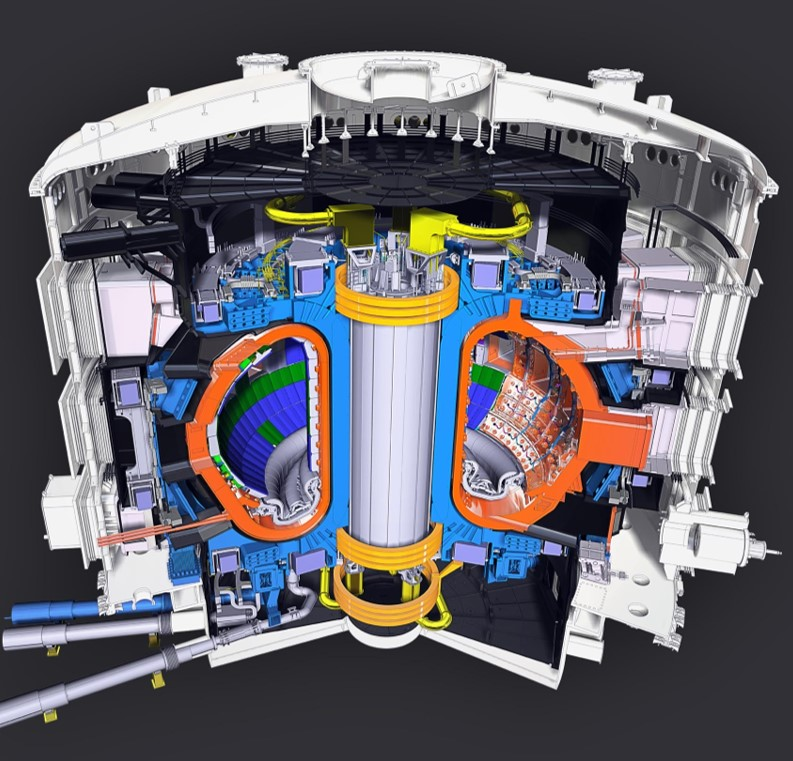
\includegraphics[width=0.6\textwidth]{schemes/ITER_2.jpg}
	\caption{Cutaway of the ITER tokamak (source: ITER Organization)}
	\label{fig:1_ITER}
\end{figure}

The limited configuration is one of the simpler magnetic configurations in a tokamak. In this setup, the plasma is in direct contact with material components which act as a limiter (see Fig. \ref{fig:WEST_limited}). It effectively splits the domain in a confined core region with closed field lines and the Scrape-Off-Layer (SOL), that extends to the wall and where field lines are open, e.g. they cross the wall. The confined plasma boundary is given by the last closed flux surface, tangential to the wall in one point. Such a configuration suffers from significant power loads on the limiters, resulting in high erosion rates and potential contamination of the plasma with impurities. The confinement is generally lower in this configuration. 

A diverted configuration, as depicted in Fig. \ref{fig:WEST_diverted}, improves the situation by a lot. The poloidal field coils shape the magnetic field lines in a fashion that they do not intersect with solid surfaces within the main plasma chamber but are instead directed to a separate region called the divertor. The last closed flux surface is then called "separatrix" and never touches the tokamak wall. The poloidal magnetic field contains now a singularity, the "X-point", and the area where the he divertor plate intecepts the continuation of the separatrix is called the "target line". The divertor handles the exhaust of heat and particles from the plasma and this configuration tends to improve overall plasma confinement and reduce impurity levels.

\begin{figure}[H]
	\centering
	\begin{subfigure}[b]{0.45\textwidth}
		\centering
		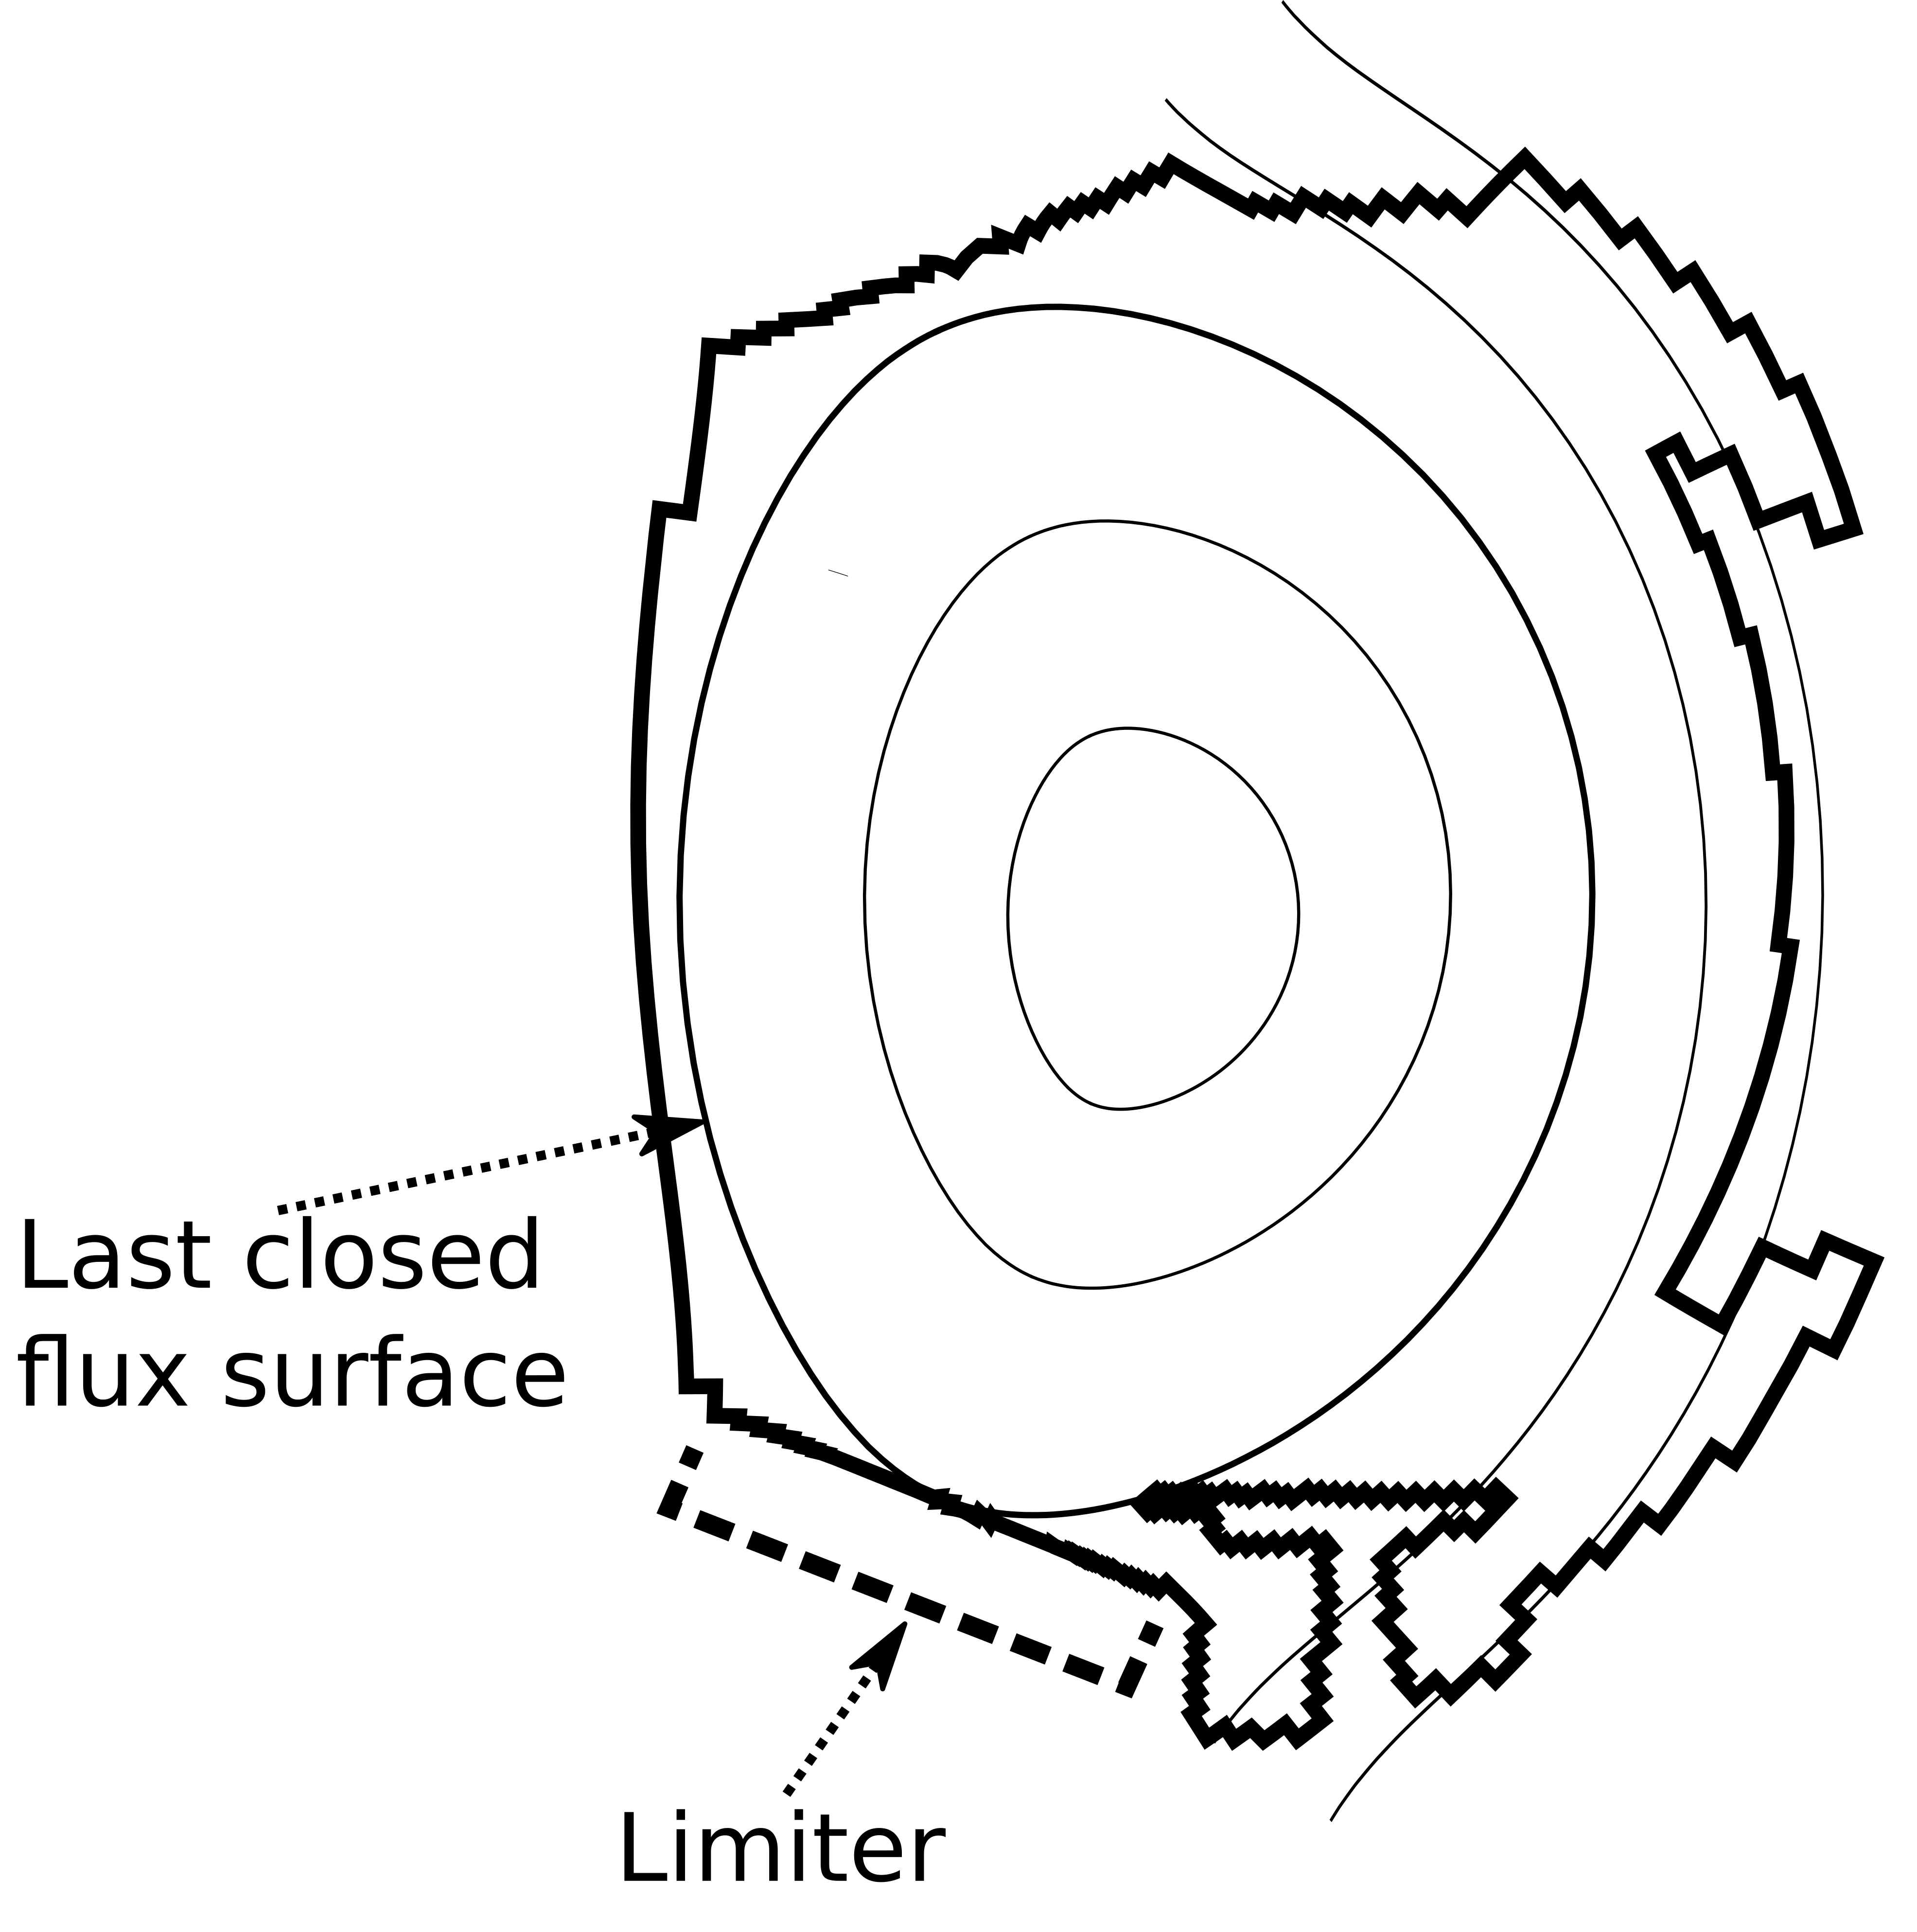
\includegraphics[height=60mm]{schemes/WESTlimited.png}
		\subcaption{Limited configuration}
		\label{fig:WEST_limited}
	\end{subfigure}
	\begin{subfigure}[b]{0.45\textwidth}
		\centering
		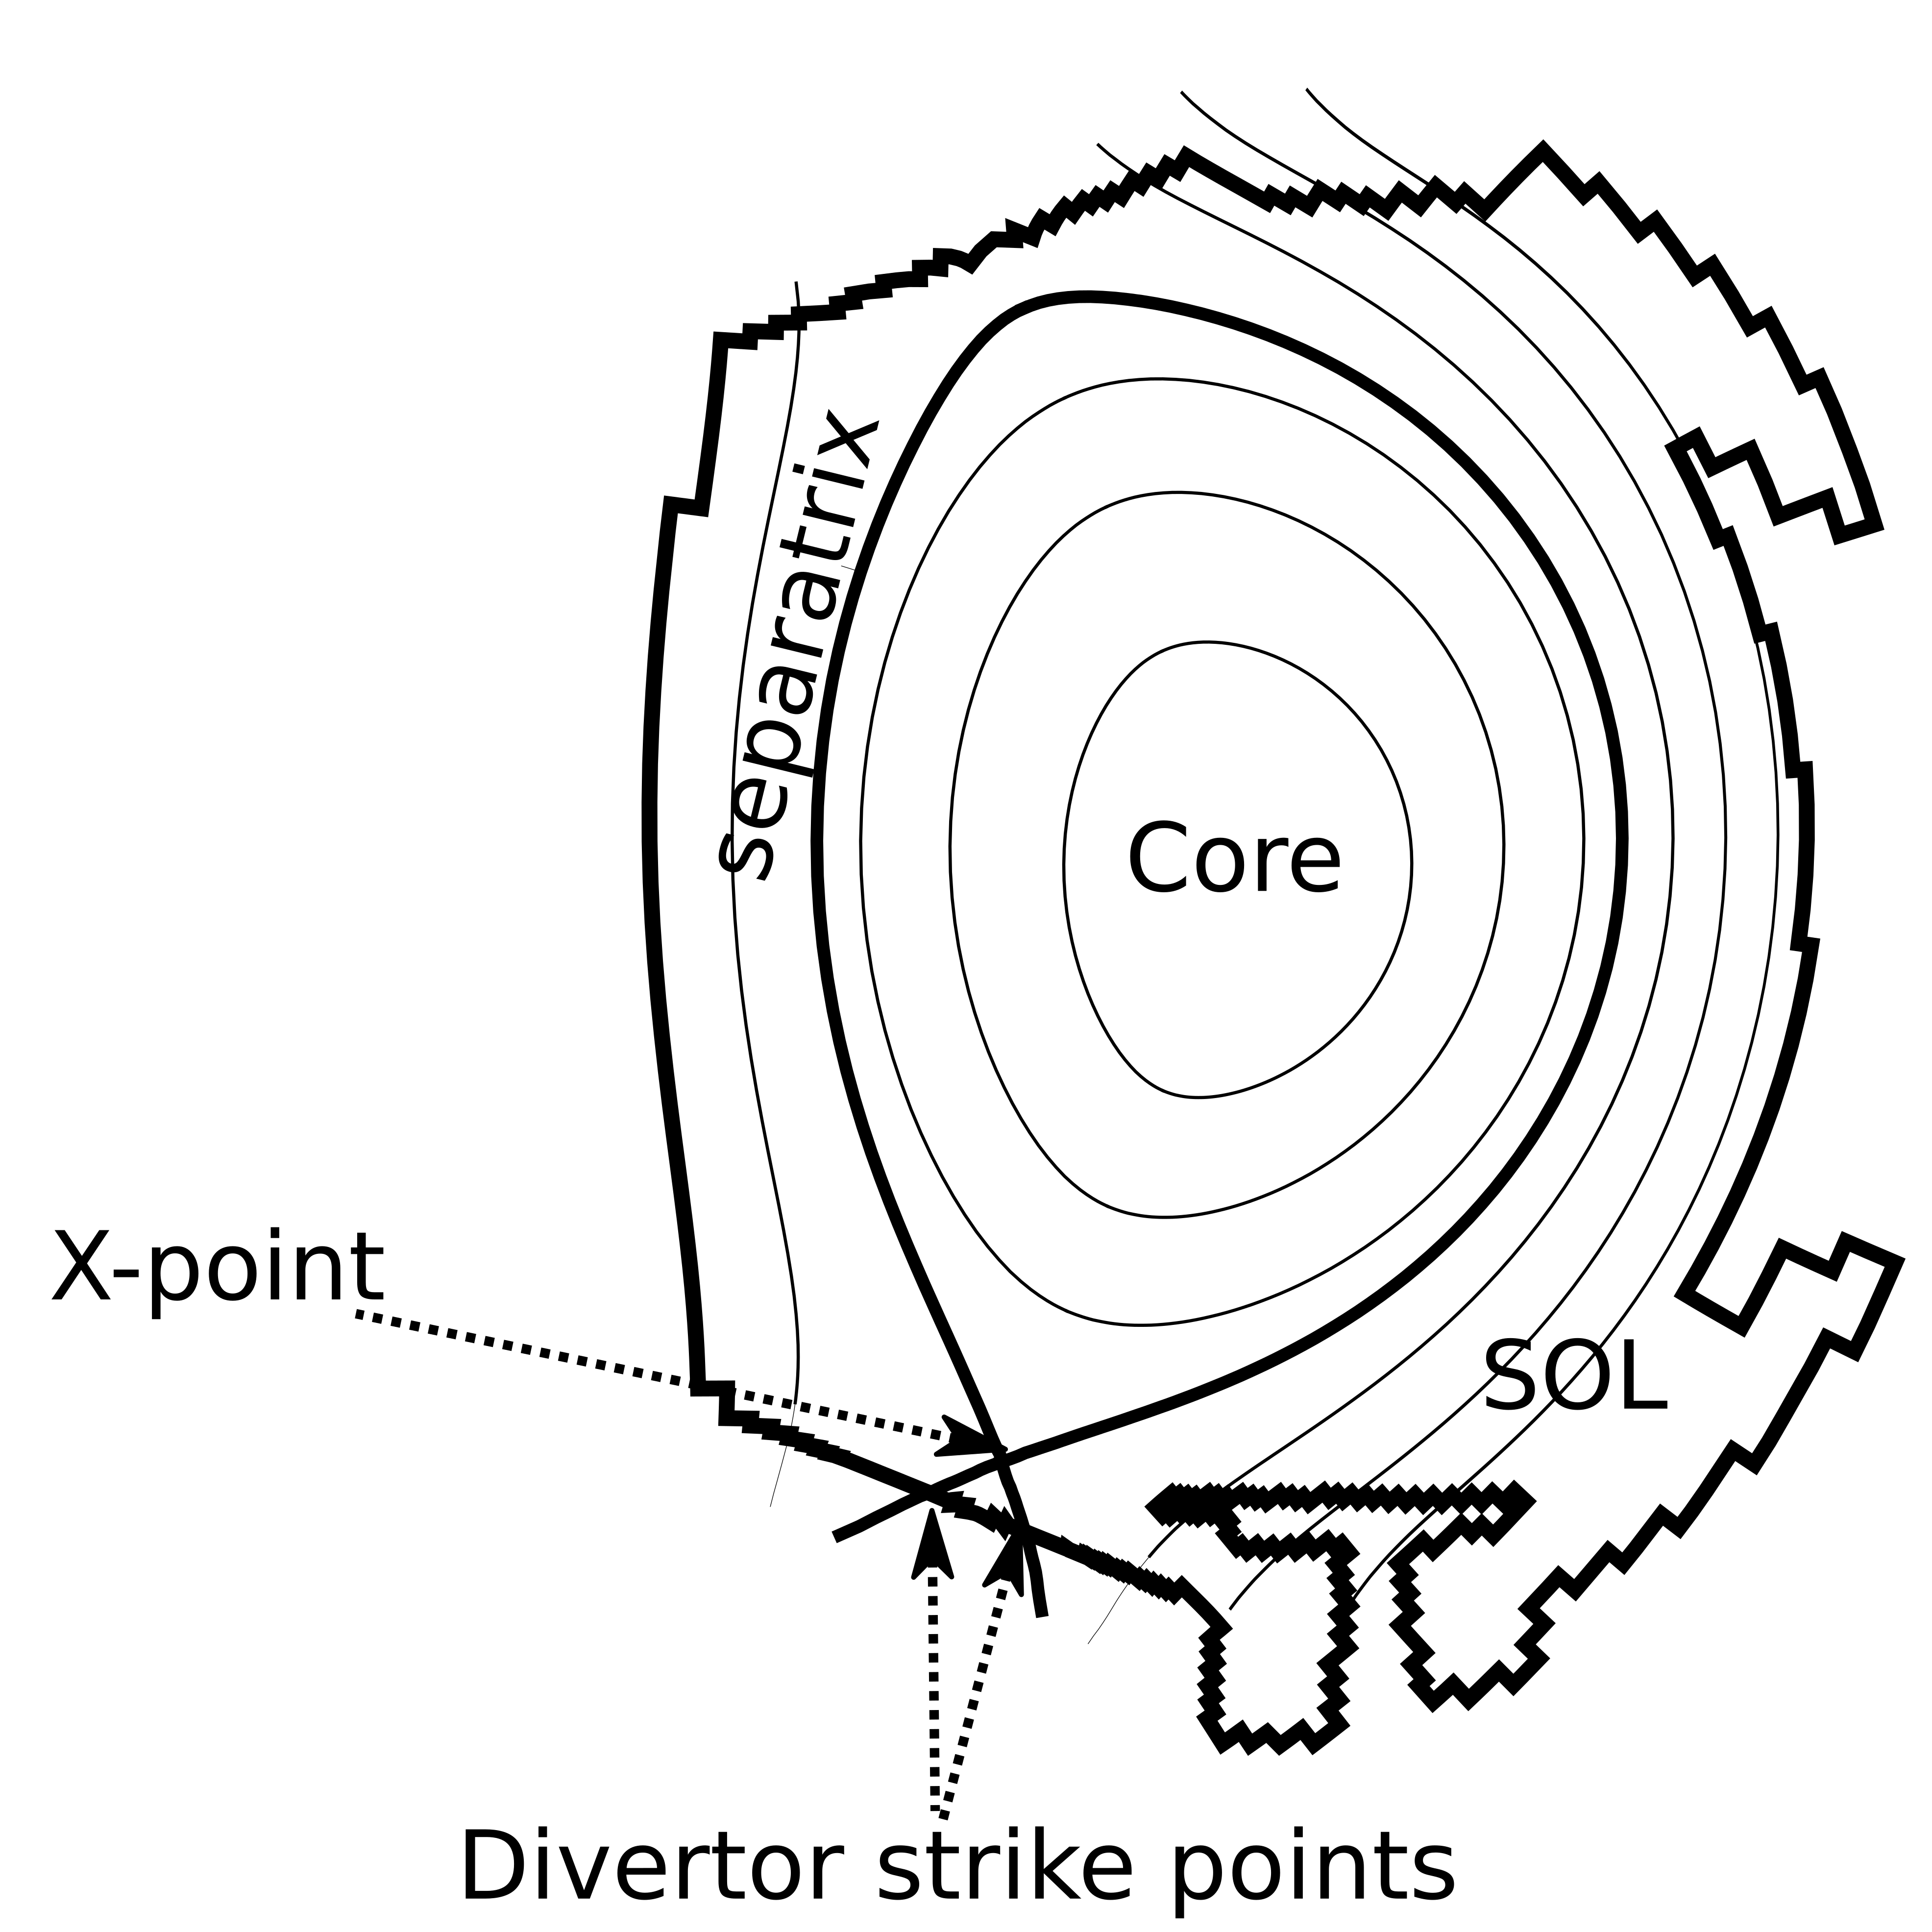
\includegraphics[height=60mm]{schemes/WESTdiverted.png}
		\subcaption{lower null configuration}
		\label{fig:WEST_diverted}
	\end{subfigure}
	\caption{Comparison of the limited and diverted configuration on a WEST geometry. }
	\label{fig:1_limdivConfigs}
\end{figure}



More exotic configurations are also feasible. In the double-null configuration, there are two divertor regions, typically located above and below the main plasma body. It splits heat loads on both divertor targets and can improve symmetry in power and particle exhaust. This symmetry helps in balancing the plasma dynamics and stabilizing the plasma, particularly with respect to vertical displacement events (VDEs), which are large-scale instabilities that can occur in tokamaks. Similarly, the X-point can be a higher-order singularity and split in more than four branches, spreading the heat load in several branches\cite{ryutov2008magnetic}. Such "snowflake" divertors can be achieved with an additional set of poloidal field coils in proximity to the divertor. Such configurations are still subject to active research in the perspective to optimize the plasma confinement and better control the heat exhaust. \\

Another important parameter of the magnetic configuration is its triangularity. It refers to the shaping of the plasma cross-section, where the plasma boundary is not circular but has an elongated shape with triangular indentations. The degree of triangularity $\delta$ measures the extent of the indentation relative to the plasma’s minor radius. High triangularity configurations can enhance plasma stability and confinement, in particular in the edge region, by allowing for higher pressure gradients.



\section{Interaction between particles}
\label{sec:intro_particlesInteration}
So far we have seen how particles are confined in magnetic field lines. It gives only a partial picture of the physical processes that occur in a tokamak. A plasma contains positively and negatively charged particles at high energetic levels and they will inevitably interact between themselves. In Sec. \ref{ssec:intro_DebyeShielding} we look at how electrons and ions organize to form a state of quasi-neutrality, in Sec. \ref{sec:intro_collisions} we dive into the mechanisms that drive particle collisions and in Sec. \ref{ssec:intro_macroscopicEffectsPlasma} we conclude how collisions translate into resistive effects.

\subsection{Debye shielding}
\label{ssec:intro_DebyeShielding}
Debye shielding refers to the macroscopic phenomenon that electric fields naturally dissipate in a plasma at rest. When a charged particle is introduced into a plasma, electrons, being lighter and more responsive than ions, quickly redistribute themselves around the introduced charge. There is then a localized region of increased electron density that counteracts the introduced electric field. The characteristic length over which this electric field is significantly attenuated is known as the Debye length $\lambda_D$:
\begin{equation}
	\label{eq:1_DebyeLength}
	\lambda_D = \sqrt{\frac{\varepsilon_0T_e}{n_ee^2}}
\end{equation}

The Coulomb potential around a point charge $Q$ exponentially decreases for distances beyond the Debye length:
\begin{equation}
	\label{eq:1_CoulombPotential}
	\Phi(r) = \frac{Q}{4\pi\varepsilon_0r}e^{-r/\lambda_D}
\end{equation}

It effectively means that at scales larger than $\lambda_D$, the plasma can be considered quasi-neutral, where the electron density compensates the charge of all present ions.
\begin{equation}
	\label{eq:1_quasiNeutrality}
	n_e = \sum_{i}q_in_i
\end{equation}



\subsection{Particle collisions}
\label{sec:intro_collisions}

At scales below the Debye length, the Coulomb force
\begin{equation}
	\mathbf{F}_C = \frac{q_1q_2}{4\pi\varepsilon_0}\frac{\mathbf{r}}{\norm{\mathbf{r}}^3}
	\label{eq:1_CoulombForce}
\end{equation}
drives collisions between two particles with charges \( q_1 \) and \( q_2 \) at a distance \( \mathbf{r} = \mathbf{r}_2 - \mathbf{r}_1 \), where \( \varepsilon_0 \) is the vacuum permittivity. By Newton's first and third laws of motion, this force defines the acceleration of each particle \( m_{1/2}\frac{d^2\mathbf{r}_{1,2}}{dt^2} = \mathbf{F}_{12/21} \) and acts in opposite directions \( \mathbf{F}_{12} = -\mathbf{F}_{21} \) for the respective particles.


Following the derivation in Chapter 3 of Hutchinson \emph{et al.}\cite{hutchinson2001introduction}, we can combine the two equations of motion to express the dynamics of a single particle (projectile) with position \( \mathbf{r} \) and reduced mass \( m_r = \frac{m_1m_2}{m_1 + m_2} \), that collides with a stationary second particle (target) at the origin. This description corresponds to a reference frame attached to the common center of mass. For an initial velocity \( \mathbf{v}_r \), the projectile will be deviated by the collision as represented in Fig. \ref{fig:TokamakBasics_collision}.

\begin{figure}[H]
	\centering
	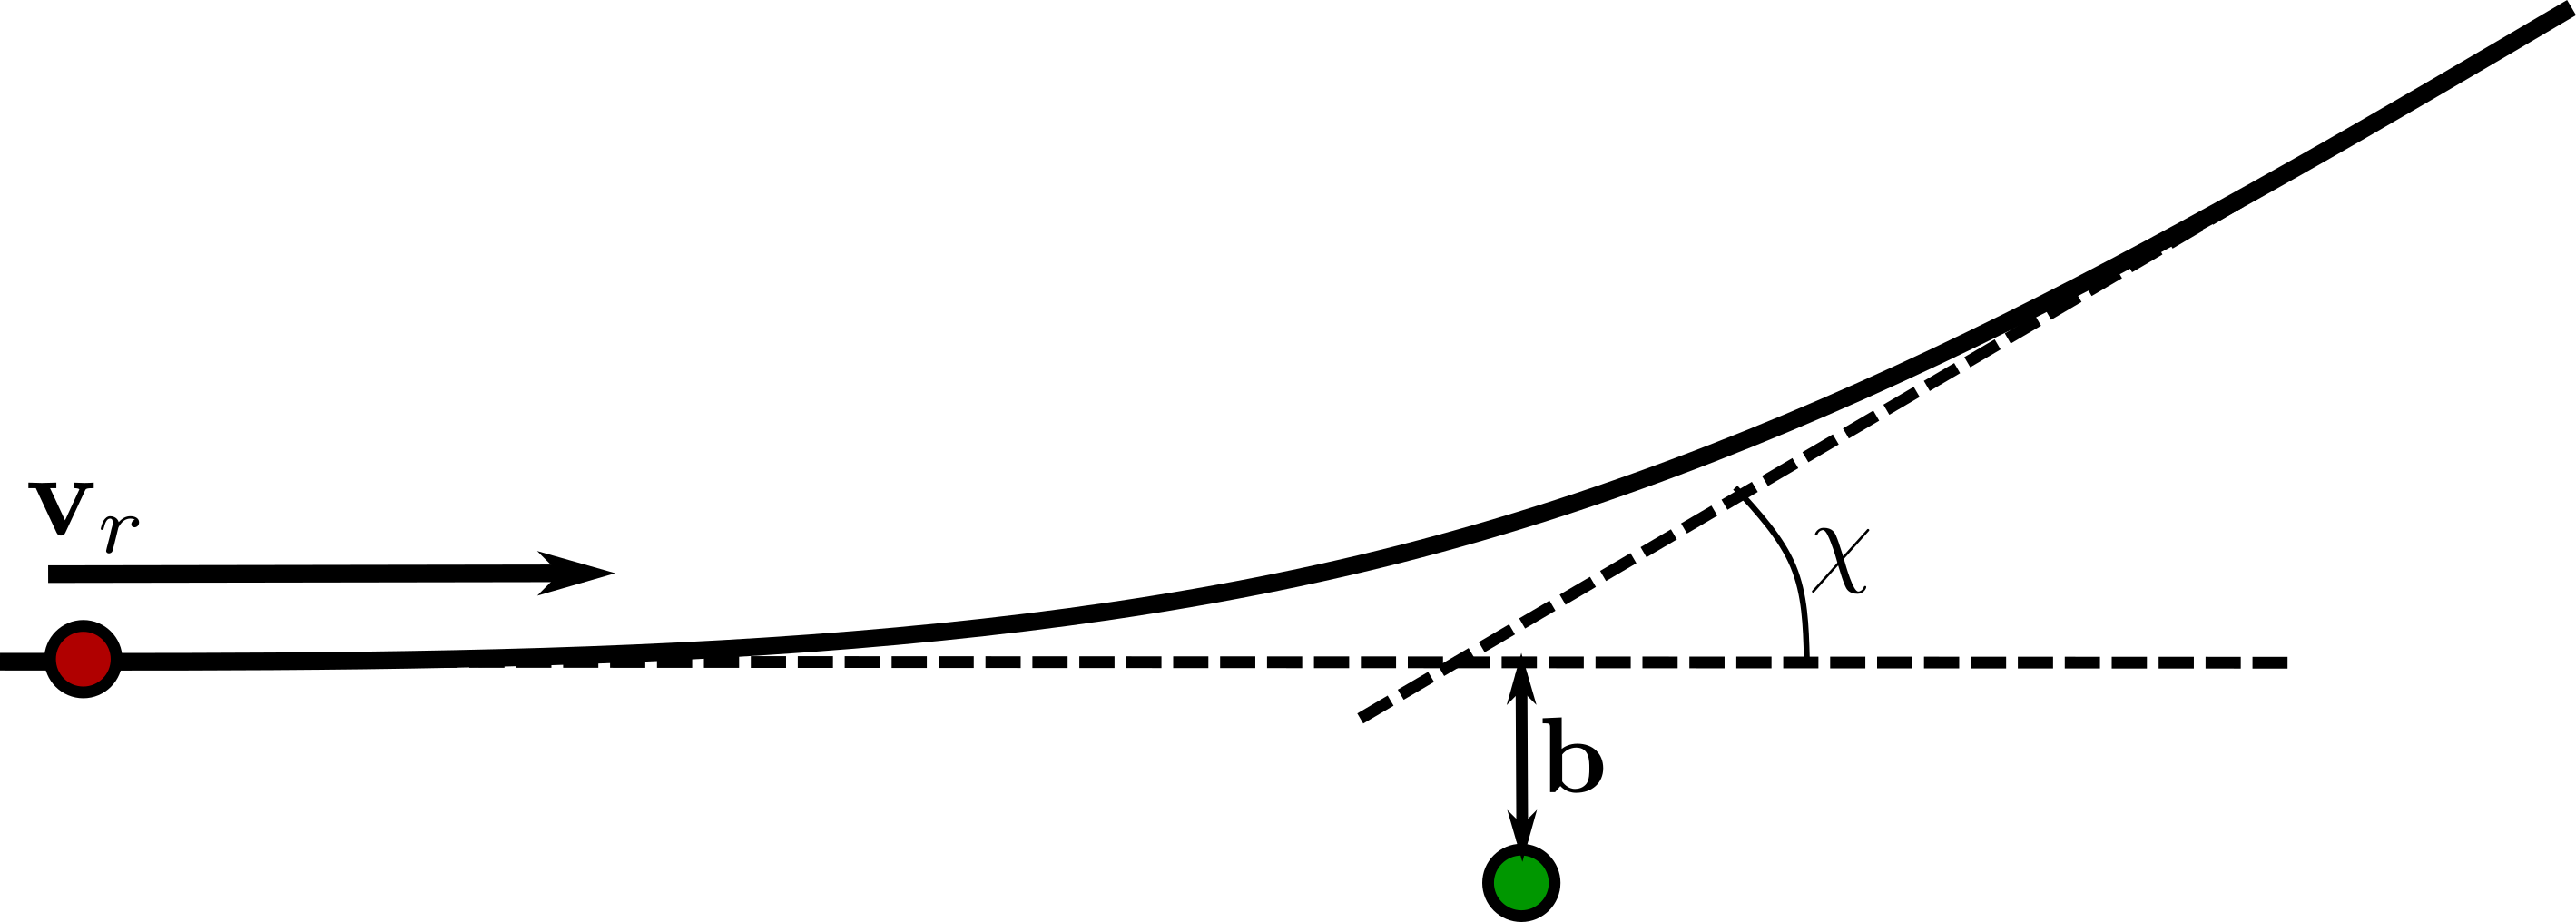
\includegraphics[width=0.62\textwidth]{schemes/collision.png}
	\caption{Trajectory of the projectile particle (red) colliding with the target particle (green). The vector \( \mathbf{b} \) denotes the impact factor and \( \chi \) is the deflection angle caused by the collision.}
	\label{fig:TokamakBasics_collision}
\end{figure}

To conserve angular momentum, the deflection of the projectile depends on the impact factor or the distance \( b = \norm{\mathbf{b}} \) of the initial trajectory to the target. Let
\begin{equation}
	b_{90} = \frac{q_1q_2}{4\pi\varepsilon_0}\frac{1}{m_r\norm{\mathbf{v}_r}^2}
\end{equation}
be the impact factor at which the projectile is deflected by a 90° angle. We can then express the deflection angle \( \chi \) at a given \( b \):
\begin{equation}
	\label{eq:1_b90}
	\chi = \tan^{-1}\frac{b_{90}}{b}
\end{equation}

This angle represents the deflection of the particle relative to the common center of mass. If we now consider two individual particles with finite mass, where the projectile approaches a stationary target with velocity \( \mathbf{v}_1 = (v_1, 0)^T \), the deflection observed in an external frame is approximately \( \chi_1 \approx \frac{m_2}{m_1 + m_2}\chi \) (using the small angle approximation). To conserve momentum in the initial direction, the target also starts moving. The projectile exits the collision with:
\begin{equation}
	\mathbf{v}'_1 = \begin{pmatrix}
		\frac{m_1v_1}{m_1 + m_2} + \frac{m_2v_1}{m_1 + m_2}\cos\chi \\
		\frac{m_2v_1}{m_1 + m_2}\sin\chi
	\end{pmatrix}
\end{equation}

At each collision, kinetic energy is transferred, and the projectile loses:
\begin{align}
	\Delta K &= K - K' = \frac{1}{2} m_1 \norm{\mathbf{v}_1}^2 - \frac{1}{2} m_1 \norm{\mathbf{v}'_1}^2 \nonumber \\
	&= \frac{2m_1^2m_2}{(m_1 + m_2)^2} v_1^2 \sin^2\frac{\chi}{2} \nonumber \\
	&\approx \frac{2m_1^2m_2}{(m_1 + m_2)^2} v_1^2 \left(\frac{b_{90}}{b}\right)^2
	\label{eq:1_particleCollision_energyLoss}
\end{align}
where the last line uses the small angle approximation \( \chi \ll 1 \).

In practice, we do not want to study every collision but are interested in the total number of collisions a particle experiences over a given length when traversing a medium with density \( n \). For that, we consider all collisions with particles at an impact factor between \( b \) and \( b + d\!b \) over a distance \( d\!x \) (see Fig. \ref{fig:TokamakBasics_collisionCrossSection}). This means we look at the volume \( V = 2\pi b d\!b d\!x \) in which we count a total of \( nV \) collisions.

\begin{figure}[H]
	\centering
	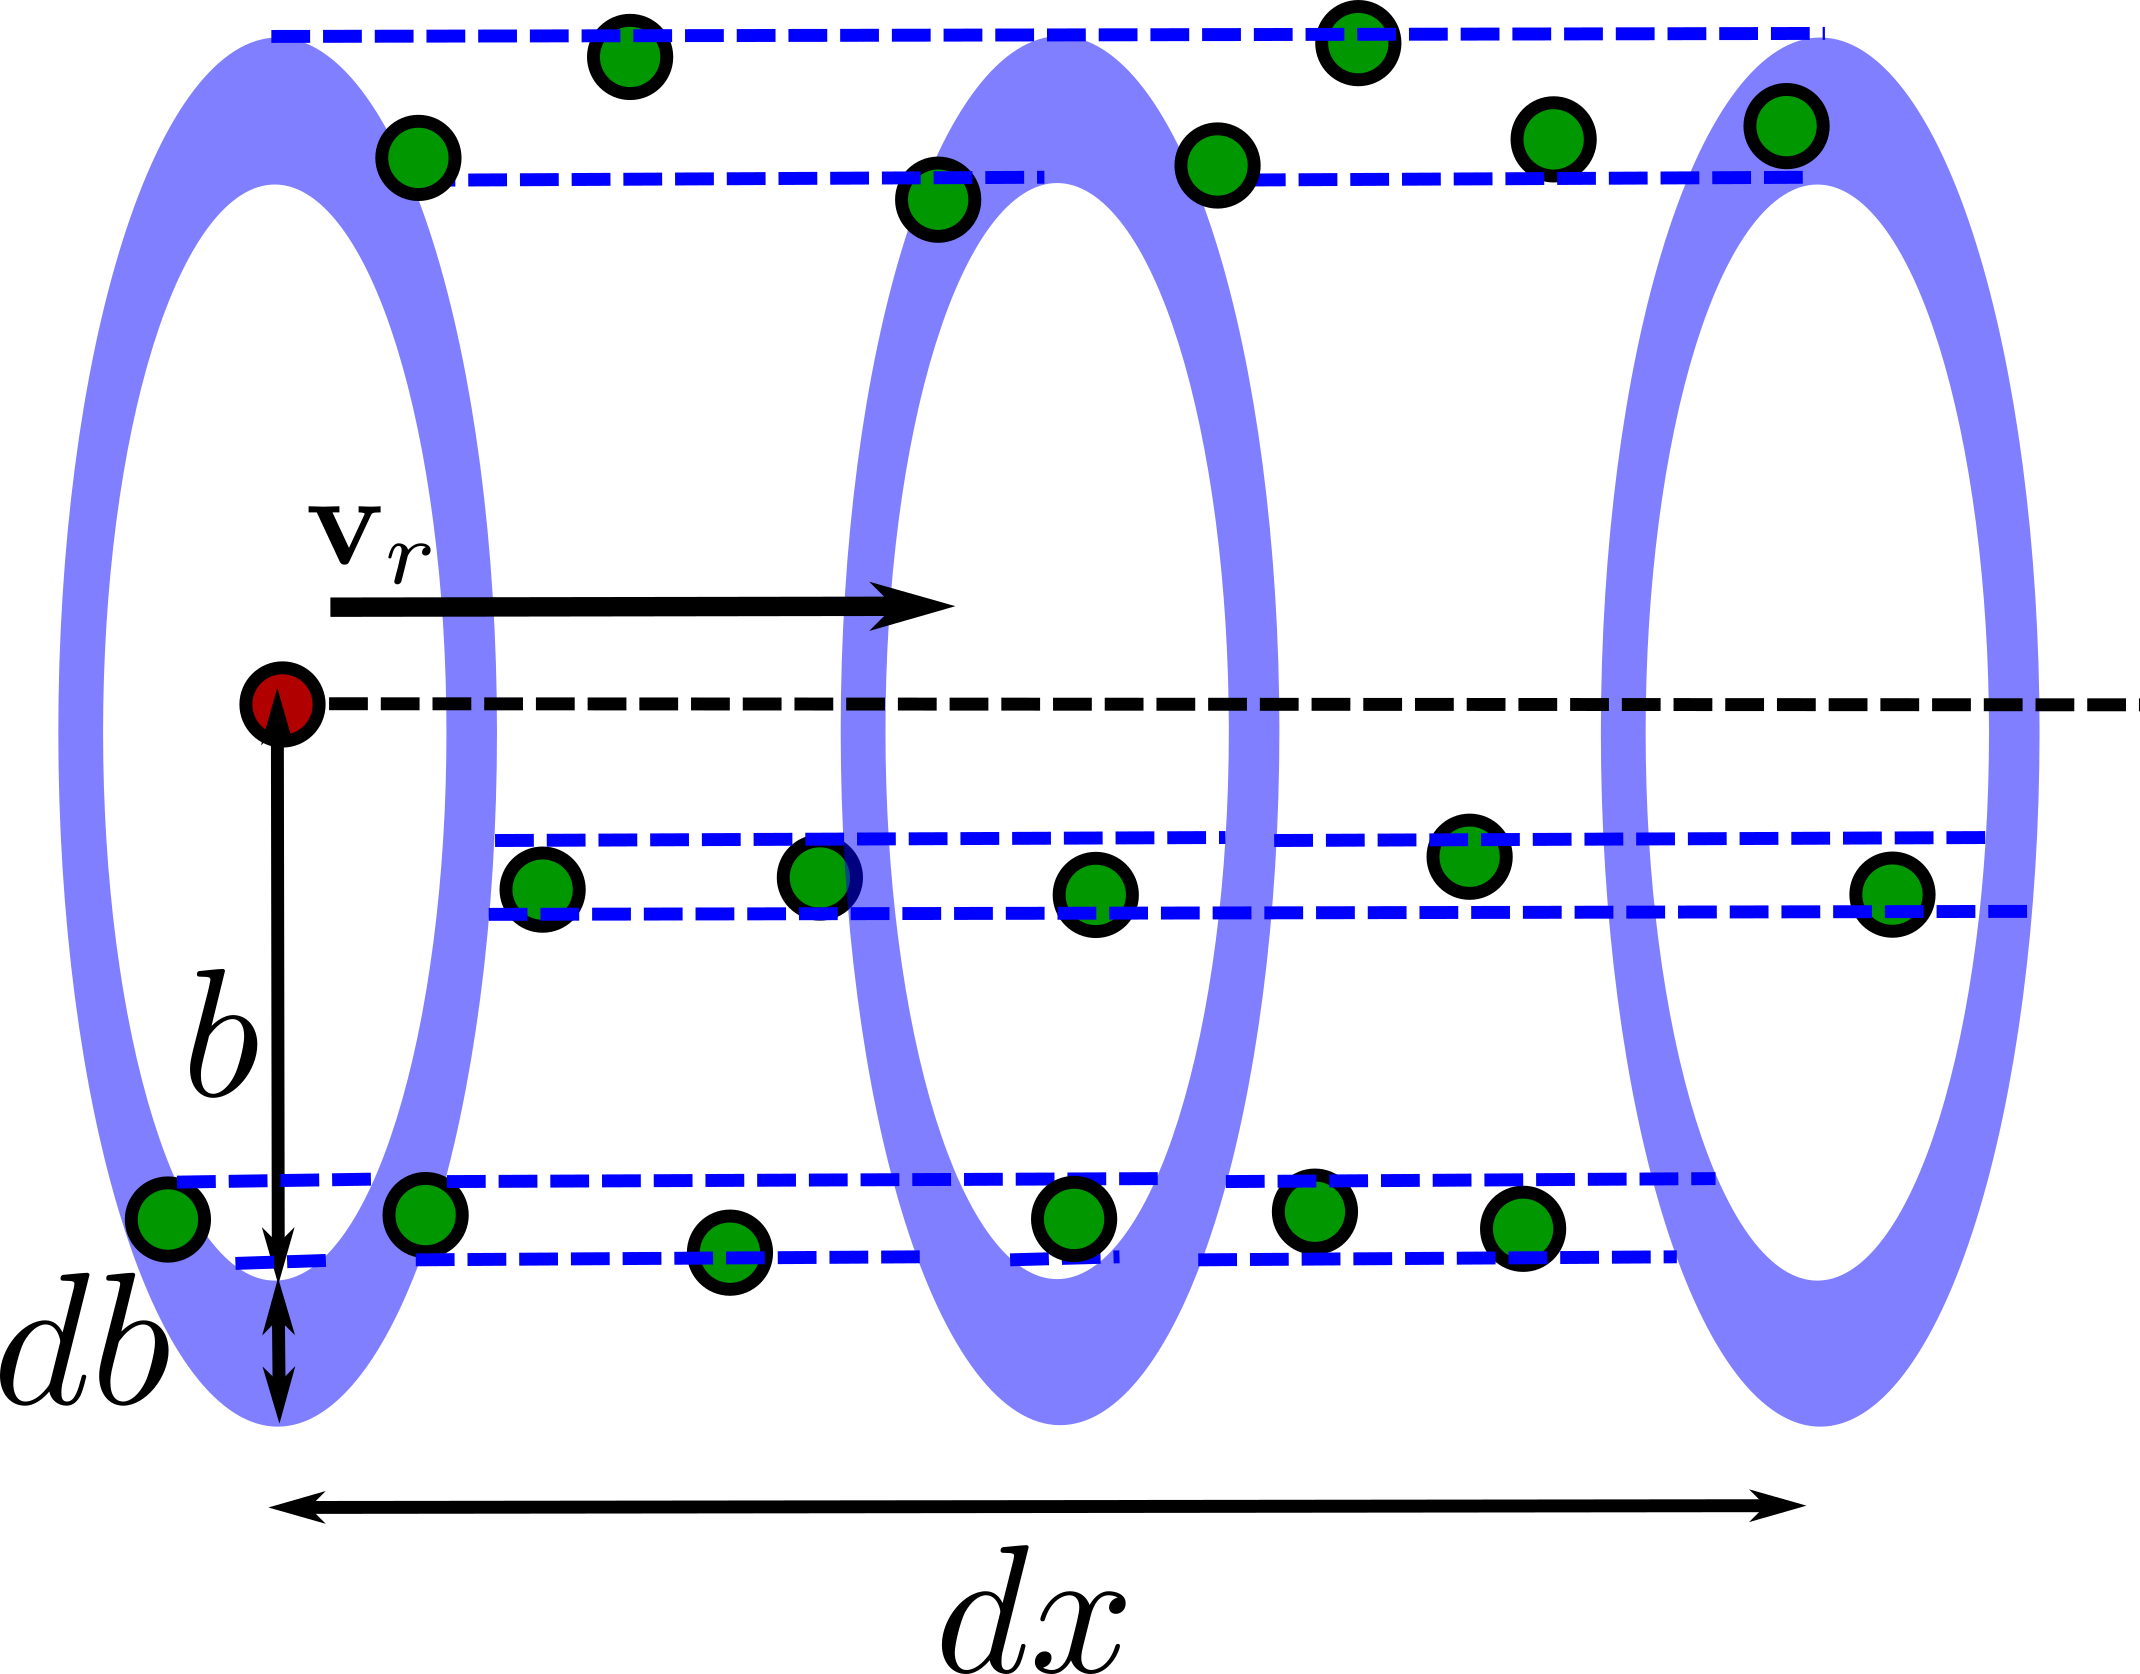
\includegraphics[width=0.45\textwidth]{schemes/collision_crossSection.png}
	\caption{Volume for given \( d\!b \) and \( d\!x \) in which collisions on the projectile are considered.}
	\label{fig:TokamakBasics_collisionCrossSection}
\end{figure}

Using Eq. \ref{eq:1_particleCollision_energyLoss} for the energy loss at each collision, we can estimate the energy our projectile loses after all collisions with the targets in the volume:
\begin{equation}
	\Delta_V K = \frac{2m_1^2m_2}{(m_1 + m_2)^2} v_1^2 \left(\frac{b_{90}}{b}\right)^2 n 2\pi b d\!b d\!x
\end{equation}

The stopping power $\frac{dK}{dx}$ describes the rate of energy loss per unit path length. It requires integrating over all possible impact factors \( b \):
\begin{equation}
	\label{eq:1_stoppingPower}
	\frac{dK}{dx} = \frac{2m_1^2m_2}{(m_1 + m_2)^2} v_1^2 n 2\pi b_{90}^2 \int_{b_{min}}^{b_{max}} \frac{1}{b} d\!b
\end{equation}

This integral diverges in both limits \( b_{min} \to 0 \) and \( b_{max} \to \infty \). We need to define cut-off values:

\begin{itemize}
	\item $b_{min} = b_{90}$ because the small angle approximation in Eq. \ref{eq:1_particleCollision_energyLoss} implies that $b>b_{90}$ \\
	\item $b_{max} = \lambda_D$ because the Coulomb potential from Eq. \ref{eq:1_CoulombPotential} vanishes quickly at distances beyond the Debye length and so does the effective Coulomb force $\mathbf{F}_C$
\end{itemize}

With these bounds, we evaluate the integral and define the Coulomb logarithm:
\begin{equation}
	\label{eq:1_CoulombLogarithm}
	\ln\Lambda = \int_{b_{90}}^{\lambda_D} \frac{1}{b} d\!b = \ln(\sqrt{\frac{\varepsilon_0T_e}{n_ee^2}}) - \ln(\frac{q_1q_2}{4\pi\varepsilon_0}\frac{1}{m_r\norm{\mathbf{v}_r}^2})
\end{equation}

For ion-ion collisions, masses $m_1 = m_2$ and charges $q_1 = q_2$ are equal. The collision frequency $\omega_c$ describes at which rate a particle loses energy through collisions relative to its total energy. The power loss is proportional to the stopping power with the particle velocity $\frac{dK}{dt} = v\frac{dK}{dx}$. We can then relate $\omega_c$ to the stopping power:

\begin{equation}
		\omega_c = \frac{v}{K}\frac{dK}{dx}
\end{equation}

If we now inject Eqs. \ref{eq:1_b90}, \ref{eq:1_stoppingPower} and \ref{eq:1_CoulombLogarithm} we obtain following expression for $\omega_c$:

\begin{align}
%	&= \frac{v}{K}\frac{2m_1^2m_2}{(m_1 + m_2)^2} v_1^2 n 2\pi b_{90}^2 \ln\Lambda \nonumber \\
%	&= \frac{v}{K}\frac{2m^2m}{(m + m)^2} v^2 n 2\pi \left(\frac{q_1q_2}{4\pi\varepsilon_0}\frac{1}{mv^2}\right)^2 \ln\Lambda \nonumber \\
%	&= \frac{vv^2 2m^3 n 2\pi }{4m^2 K} \frac{q^4}{16\pi^2\varepsilon_0^2m^2v^4}\ln\Lambda \nonumber \\
%	&= \frac{q^4 n }{16\pi m v K \varepsilon_0^2}\ln\Lambda \nonumber \\
	\omega_c&= \frac{q^4 n}{16\pi \varepsilon_0^2 \sqrt{2m}K^{3/2}}\ln\Lambda \label{eq:1_collisionFrequency}
\end{align}
Assuming that the kinetic energy follows directly the plasma temperature with the relation $K = 3/2T$, we can express the characteristic collision time $\tau_c$ and mean free path $\lambda_c$:
\begin{align}
%	\tau_c &= \frac{1}{\omega_c} = \frac{16\pi \varepsilon_0^2 \sqrt{2m}(3/2T)^{3/2}}{q^4 n \ln\Lambda} 	\nonumber \\
	\tau_c = \frac{1}{\omega_c} &= \frac{52\sqrt{3}\pi \varepsilon_0^2\sqrt{m}}{q^4 \ln\Lambda} \frac{T^{3/2}}{n}\label{eq:1_collisionTime} \\
%	\lambda_c &= \frac{v}{\omega_c} = \frac{16\pi \varepsilon_0^2 \sqrt{2m}vT^{3/2}}{q^4 n \ln\Lambda} \nonumber \\
%	&= \frac{16\pi \varepsilon_0^2 \sqrt{2m}(2K/m)^{1/2}T^{3/2}}{q^4 n \ln\Lambda} \nonumber \\
%	&= \frac{32\pi \varepsilon_0^2 (K)^{1/2}T^{3/2}}{q^4 n \ln\Lambda} \nonumber \\
%	&= \frac{32\pi \varepsilon_0^2 (3/2T)^{1/2}T^{3/2}}{q^4 n \ln\Lambda} \nonumber \\
	\lambda_c = \frac{v}{\omega_c} &= \frac{32 \sqrt{3/2}\pi \varepsilon_0^2}{q^4 \ln\Lambda}\frac{T^2}{n} \label{eq:1_meanFreePath}
\end{align}

It is worth noting that $\tau_c$ is proportional to $T^{3/2}/n$ and $\lambda_c$ to $T^2/n$ as all other terms are near-constant for a given ion in a tokamak.


\subsection{Macroscopic effects of plasma collisions}
\label{ssec:intro_macroscopicEffectsPlasma}

As particles collide, energy is transferred from faster-moving to slower-moving particles, which, at a macroscopic scale, corresponds to heat conduction. Spitzer and Härm developed a model for plasmas in a near-equilibrium state\cite{SpitzerResistivity}, where deviations from the Maxwellian particle distribution due to the temperature gradient is small. The heat flux is then inversely proportional to the temperature gradient:

\begin{equation}
	q = -\kappa_{SH} \grad T
\end{equation}

In a weakly collisional regime, the thermal conductivity $\kappa_{SH}$ then corresponds to the rate at which energy is transported and is proportional to its speed $v_{th}$ and the distance transported before the next collision $\lambda_c$. From the previous discussion on collisions, $\kappa_{SH}$ then depends on the electron temperature $T_e$ taken to the exponent $5/2$:

\begin{equation}
	\kappa_{SH} \propto \frac{T_e^{5/2}}{Z \ln \Lambda}
\end{equation}

In a similar fashion, weak collisionality results in viscous effects. Alike energy, momentum is transferred from fast to slow particles, whereby velocity gradients are reduced over time. The particle flow is overall smoothened and becomes more uniform. The resultant viscous force

\begin{equation}
	F = \nu_{SH}\grad v
\end{equation}

depends on the velocity gradient. The same reasoning as for the conductivity holds for the viscosity and we can express:

\begin{equation}
	\nu_{SH} \propto \frac{T_e^{5/2}}{Z^4 \ln \Lambda}
\end{equation}

Finally, collisions scatter electrons, with the effect to impend the current flow. This translates into electric resistivity $\eta_{SH}$, which is directly proportional to the collision frequency $\omega_c$. We then have:

\begin{equation}
	\eta_{SH}\propto\frac{Z \ln \Lambda}{T_e^{3/2}}
\end{equation}

Plasma resistivity is essential to understand current flow and Ohmic heating. As the plasma heats up, collisions are less frequent, and it becomes a more efficient conductor. Characteristic times for heat conductivity and resistivity are of the order of the electron-ion collision time $\tau_c$ at around $10^{-5}$s while viscosity occur on the the much slower scale of the ion-ion collision time, which reaches up to a few milliseconds. 



\section{Scrape-Off-Layer}
\label{sec:intro_SOL}

As presented in Sec. \ref{ssec:intro_limitedDivertedConfig}, the magnetic configuration in tokamaks can be split in two main regions: the core with closed magnetic field lines and the the scrape-off-layer (SOL) with open field lines. The properties of the latter are important to describe the plasma and to design a nuclear fusion device. Where magnetic field lines penetrate the material wall, the sheath, described in Sec. \ref{sec:intro_sheath}, strongly alters the physical properties of the plasma. It is followed by a discussion in Sec. \ref{ssec:intro_heatExhaust} on the particle and heat fluxes at the wall and an introduction to the impact of SOL physics on plasma confinement. 



\subsection{Fundamental sheath physics}
\label{sec:intro_sheath}

The SOL is characterized by open flux surfaces and where magnetic field lines cross the wall, the quasi-neutrality assumption from Sec. \ref{ssec:intro_DebyeShielding} does not hold anymore. The much lighter electrons travel much faster towards the wall (about $\sqrt{m_i/m_e}$ faster than ions), creating a net negative charge in the direct proximity to the wall. It is not until a few Debye lengths $\lambda_D$ before shielding restores known plasma conditions forming a region known as "electrostatic sheath". The negative charge attracts ions and repulses electrons, and we can assume that the electron density decreases exponentially approaching the wall. This eventually leads to the Bohm criterion\cite{riemann1991bohm}, which states that at the sheath entrance the ion speed must be equal or larger than the sound speed of the plasma.

\begin{equation}
	\label{eq:intro_BohmCriterion}
	v_{se} \ge c_s = \sqrt{\frac{T_i+T_e}{m_i}}
\end{equation}

From there, it is possible to calculate a sheath particle flux:
\begin{equation}
	\gamma_{se} = nv_{se}
\end{equation}

and a heat flux:

\begin{equation}
	q_{se} = \gamma n T \gamma_{se}
\end{equation}
with the sheath transmission coefficient $\gamma$. As the sheath is not collisional, these coefficients have to be determined from kinetic theory\cite{Stangeby_2000}. For hydrogen plasma, it is common to take the values $\gamma_i = 2.5$ for ions and $\gamma_e = 4.5$ for electrons.


\subsection{Problematic of heat exhaust}
\label{ssec:intro_heatExhaust}
An important part of the heat produced in a tokamak, whether it originates from external heating or from the fusion reaction, is evacuated by hot plasma particles. Cross-field transport allows confined particles from the hot core to cross the separatrix. As they enter the SOL, they follow the magnetic field lines until they impact the divertor on the thin target band. This region is extremely critical as large amounts of power are directed on a fairly small area. It is projected for ITER that heat loads at the targets are very close to material limits\cite{gunn2017surface}. The peak heat flux $q_{peak}$ could reach values over $10MW/m^2$. For a safe tokamak operation, it is essential to well understand and predict heat fluxes on the strike points. An important metric to take into the consideration is the heat flux o power fall-off width $\lambda_q$. It describes the spread of the heat flux on the divertor targets, and a larger value allows to spread the power exhaust on a larger area. It allows to describe the heat flux at a distance $r$ from the target:

\begin{equation}
	q(r) =  q_{peak}e^{-\frac{r}{\lambda_q}}
\end{equation}

Eich \emph{et al.}\cite{eich2013scaling} developed a scaling law to estimate $\lambda_q$ for H-mode operation based on machine parameters. It states that the width is inversely proportional to the toroidal magnetic field $\lambda_q\propto B_\varphi^{-0.8}$, meaning that larger machines with stronger coils will also have a thinner target line. 











	\chapter{Description of Plasmas}
\label{chap:PlasmaSimulations}

\vfill
\begin{chaptersummarybox}
	The kinetic description of plasmas applies the Lorentz equation to distribution functions $f$ of particle densities and velocities with appropriate collision operators.
	\begin{equation*}
		\pdv{f}{t} + \mathbf{v} \cdot \nabla_{\mathbf{x}} f + \frac{\mathbf{F}}{m} \cdot \nabla_{\mathbf{v}} f = C_{\text{coll}} + C_{\text{other}}
	\end{equation*}
	From this, conservation equations for mean quantities can be derived for density, momentum, and energy, with fluid closures to avoid higher-order moments. These equations are coupled to Gauss's, Ampère's, and Faraday's laws for magnetism.
	\begin{gather*}-
		\partial_t n + \grad\cdot\left(n\mathbf{v}\right) = S_n \qquad\qquad
		mn\left(\partial_t \textbf{v} + \textbf{v}\cdot\grad\textbf{v} \right) = -\grad p + \textbf{F} \\
		\partial_t p+\textbf{v}\cdot\grad p + \frac{5}{3}p\grad\cdot\textbf{v} = \frac{2}{3}\grad\cdot\textbf{Q}+S_E  \\
		\grad\cdot\textbf{B} = 0  \qquad\qquad \grad\cross\textbf{B} = \mu_0 \textbf{j}  \qquad\qquad \partial_t \textbf{B} = \grad\cross\left(\textbf{v}\cross\textbf{B} - \eta\textbf{j}\right) + S_\textbf{B}
	\end{gather*}
	In drift-reduced fluid models, MHD equations are projected onto the parallel direction, where the drift-ordering assumption allows to incorporate plasma drifts  in the advection terms and finite-Larmor radius effects. These models are well-suited to simulate drift-wave and interchange instabilities in the tokamak edge. Turbulence arises from electrostatic potential fluctuations  to density fluctuations in the non-adiabatic electron response in Ohm's law. These instabilities are characterized by collisional (resistive), inertial, and inductive effects, with associated parameters:
	\begin{align*}
		C &= \eta\left(\frac{qR}{L_\perp}\right)^2	&
		\mu_{eff} &= \frac{m_e}{m_i}\left(\frac{qR}{L_\perp}\right)^2 &
		\beta_{eff} &= \beta\left(\frac{qR}{L_\perp}\right)^2
	\end{align*}
	The interplay between these parameters determines whether the turbulence is driven by collisional, electron inertial, or electromagnetic effects.
\end{chaptersummarybox}
\vfill
\newpage


The difficulty in obtaining global experimental measurements in tokamaks requires complementary numerical simulations. Currently, these numerical data are essential to complement experimental measurements and support their interpretation. In the longer term, they will be used to make predictions and support the design of ITER experiments. Self-consistent simulations of the plasma edge are challenged by a complex geometry and the variety of involved scales. The magnetic equilibrium exhibits both open and closed magnetic field lines, breaking the toroidal symmetry. Turbulent fluctuations typically have sizes on the order of the ion gyroradius $\rho_\alpha$ ($\ge 0.4\, \text{mm}$)\cite{hennequin2004} in the perpendicular direction to the magnetic field lines, and compete with phenomena occurring along them on the order of the parallel connection length $\propto q_s R_0$ (where $q_s$ is the safety factor, and $R_0$ the tokamak major radius), which can extend up to 100 meters. \\

This chapter presents the different approaches to describe plasma self-consistently. In a first section \ref{sec:desc_modelHierarchy}, we explain the steps how the Lorentz force can be successively rewritten in a kinetic equation and in a conservation equations on mean plasma quantities. We extend the discussion in Sec. \ref{sec:edge_driftWaves} to drift-reduced fluid models that are commonly used for turbulent plasma simulations of the tokamak edge. Finally, we analyze in Sec. \ref{sec:edge_DAW} from a theoretical point of view the impact of electromagnetic effects on drift-wave turbulence in our models. 


\section{A hierarchy of models}
\label{sec:desc_modelHierarchy}

Plasmas can be modeled using various sets of equations that trade off between accuracy and computational feasibility. Generally, more accurate models are prohibitively expensive and are beyond the capabilities of current high-performance computing (HPC) infrastructure when applied to large systems. Depending on the scientific objective, high-fidelity models will accurately capture physical processes while reduced models complement this with full-scale simulations at relevant time scales. In this chapter, we introduce the major approaches that are used nowadays, with a special care to highlight how they are connected and where they differ. The most comprehensive approach in Sec. \ref{sec:desc_directDesciption} rely on plasma particles themselves or their statistical distribution. From there, the Chapman-Enskog expansion in Sec. \ref{sec:desc_fluidMoments} allows to express conservation equations on averaged plasma quantities and lay the foundations for fluid models. Finally, MHD models in Sec. \ref{sec:desc_MHD} offer a framework to combine those conservation equations with the evolution of electromagnetic properties of the plasma. 

\subsection{Direct description of plasma particles}
\label{sec:desc_directDesciption}
Particles are the foundation of the first set of models. They can either be solved individually as in Sec. \ref{ssec:desc_particleTracking} or represented by their distribution functions in the so-called kinetic models (Sec. \ref{ssec:desc_kineticModels}).

\subsubsection{Particle tracking}
\label{ssec:desc_particleTracking}
In the most general description, each particle in a tokamak—whether neutron, ion, atom, or electron—is represented individually with three degrees of freedom for both position $\mathbf{x}$ and velocity $\mathbf{v}$. The system's dynamics are governed by the Lorentz force:
\begin{align}
	\pdv{\mathbf{v}}{t} &= \mathbf{F} = q\mathbf{E} + q\mathbf{v} \times \mathbf{B} \label{eq:desc_particle}\\
	\pdv{\mathbf{x}}{t} &= \mathbf{v}
\end{align}
where $\mathbf{E}$ is the electric field, $\mathbf{B}$ the magnetic field, and $q$ the charge of the particle. \newline
Given that a medium-sized tokamak like WEST contains approximately $N_p \approx 10^{20}$ particles, each with six degrees of freedom, direct numerical simulation is infeasible. Computational effort can be reduced by using macro-particles, which represent many real particles. A prominent approach utilizing this concept is the particle-in-cell (PIC) method\cite{tskhakaya2007particle}, where macro-particles evolve in pre-calculated fields on a mesh or interact directly with one another. PIC methods are employed to study phenomena such as collisions with neutral particles\cite{birdsall1991particle}, plasma-wall interactions\cite{khaziev2018hpic}, or instabilities induced by fusion products\cite{cook2013particle}.



\subsubsection{Kinetic models}
\label{ssec:desc_kineticModels}
As a further abstraction, an ensemble of particles can be described statistically through a distribution function $f(\mathbf{x}, \mathbf{v},t)$. This kinetic description replaces individual particles with a probability distribution, avoiding the need to calculate exact positions and velocities at each moment in time. The behavior of the distribution function is governed by the Boltzmann equation:
\begin{equation}
	\label{eq:BoltzmannEquationKineticDescription}
	\pdv{f}{t} + \mathbf{v} \cdot \nabla_{\mathbf{x}} f + \frac{\mathbf{F}}{m} \cdot \nabla_{\mathbf{v}} f = C_{\text{coll}} + C_{\text{other}}
\end{equation}
where $C_{\text{coll}}$ represents the collision operator, handling Coulomb collisions as introduced in Sec. \ref{sec:intro_collisions}, and $C_{\text{other}}$ includes additional source terms. Substituting the force vector $\mathbf{F}$ with the Lorentz force (Eq. \ref{eq:desc_particle}) yields the Vlasov equation. \newline

To achieve sufficient accuracy, approximately $N_x = 10^9$ spatial discretization points and $N_\sigma = 10^6$ points for the distribution function are required. Considering that both position and velocity have three components each, this results in $6 \cdot 10^{15}$ degrees of freedom—significantly fewer than in the particle description. \newline

Further simplification is achieved through the gyrokinetic approach. While particles in a plasma predominantly follow magnetic field lines, their motion forms a helical trajectory characterized by the Larmor frequency and radius:

\begin{equation}
	\omega_L = \frac{eZB}{m} \qquad\qquad l_L = \frac{mv_\perp}{eZB}
\end{equation}

This allows the elimination of one degree of freedom in the distribution function, as the velocity can be described by its parallel component $v_\parallel$ along the magnetic field line and its perpendicular component $v_\perp$. This simplification is valid only when the Larmor frequency and radius are much smaller than any characteristic frequency or length in the system, which is typically true in the core of the tokamak but not in the scrape-off layer (SOL), where the gyrokinetic approach is less suitable. \\

Gyrokinetic models are particularly useful to study transport barriers and turbulence driven by ion and electron temperature gradients (ITG/ETG) or trapped electron mode (TEM) instabilities and typically use full-\textit{f} turbulence models. The code GYSELA\cite{grandgirard2007global,grandgirard20165d} follows a semi-Lagrangian method to study core turbulence, zonal flows an neoclassical transport and is capable of relatively long simulated plasma times. Plasma-wall interactions and kinetic neutrals make XGC\cite{hager2022} particularly well-suited for edge and SOL turbulence. It allowed for comprehensive divertor heat exhaust studies\cite{chang2017gyrokinetic} and is capable of complex 3D magnetic configurations found in stellarators\cite{cole2019verification}. The Eulerian code GENE-X\cite{goerler2011global,michels2021gene} is ideal for full-\textit{f} electromagnetic simulations of turbulence at multiple scale in the core-edge region. 


\subsection{Three fluid moments of the kinetic equation}
\label{sec:desc_fluidMoments}
Deriving transport equations for plasma quantities analogous to the Navier-Stokes equations in classical fluid dynamics is highly desirable. Such an approach would enable the use of established computational fluid dynamics (CFD) methods for turbulence modeling, significantly reducing the number of degrees of freedom. Starting with the distribution function $f$, the $k$-th moment of the transport equation is obtained by applying the tensor product $\mathbf{v} \otimes \dots$ $k$ times and then integrating over the velocity:

\begin{equation}
	\mathcal{M}^k = \int_\mathbf{v} f\mathbf{v}^k d\mathbf{v}^3
\end{equation}

Substituting the kinetic equation \ref{eq:BoltzmannEquationKineticDescription} into this expression yields the following equation for the $k$-th moment:

\begin{align}
	\partial_t \int_\mathbf{v} f\mathbf{v}^k d\mathbf{v}^3 + \int_\mathbf{v} \mathbf{v}^k \mathbf{v} \cdot \nabla_{\mathbf{x}} f d\mathbf{v}^3 + \int_\mathbf{v} \mathbf{v}^k \frac{\mathbf{F}}{m} \cdot \nabla_{\mathbf{v}} f d\mathbf{v}^3 &= \int_\mathbf{v} \mathbf{v}^k C d\mathbf{v}^3 \nonumber \\
	\partial_t \mathcal{M}^k + \nabla_{\mathbf{x}} \cdot \mathcal{M}^{k+1} - \frac{k}{m} \mathbf{F} \otimes \mathcal{M}^{k-1} &= \int_\mathbf{v} \mathbf{v}^k C d\mathbf{v}^3 \label{eq:desc_generalMomentsEq}
\end{align}

Expressing the $k$-th moment requires knowledge of the $k-1$-th and $k+1$-th moments. Consequently, a fully consistent plasma description would require infinitely many equations, which is impractical. Therefore, we typically consider only the first three moments, using fluid closures to compensate for the missing higher-order equations. These moments effectively allow us to replace a particle-based description with averaged quantities:

\begin{align}
	&\text{Particle density:} & \mathcal{M}^0 &= n = \int_\mathbf{v} f d\mathbf{v}^3 && \left[\text{m}^{-3}\right] \\
	&\text{Momentum density:} & \mathcal{M}^1 &= \boldsymbol{\gamma}  = n \mathbf{u} = \int_\mathbf{v} f \mathbf{v} d\mathbf{v}^3 && \left[\text{m}^{-2} \cdot \text{s}^{-1}\right] \\
	&\text{Pressure tensor:}   &  m \mathcal{M}^2 &= \boldsymbol{\Pi} = m \int_\mathbf{v} f \mathbf{v} \otimes \mathbf{v} d\mathbf{v}^3 && \left[\text{kg} \cdot \text{m}^{-1} \cdot \text{s}^{-2}\right]
\end{align}

where $\mathbf{u}$ is the fluid velocity and $m$ the particle mass. This framework sets the stage for deriving the three fundamental conservation equations for fluid models of plasmas.



\subsubsection{Mass conservation (\textit{k} = 0)}

Starting from Eq. \ref{eq:BoltzmannEquationKineticDescription}, the mass balance equation for the unknowns $n$ and $\mathbf{u}$ is derived as follows:
\begin{equation}
	\label{eq:ZeroMomentTransportEquation}
	\partial_t n + \nabla \cdot (n\mathbf{u}) = S_n
\end{equation}
This equation provides one relation but involves four unknowns, necessitating additional equations to fully describe the system. The term $S_n$ accounts for particle sources arising from non-elastic collisions in $C_{\text{other}}$, such as ionization or recombination processes.

\subsubsection{Momentum conservation (\textit{k} = 1)}

For the first moment equation, we multiply the Boltzmann equation \ref{eq:BoltzmannEquationKineticDescription} by $\mathbf{v}$ and integrate over the velocity space, yielding:
\begin{equation}
	\partial_t \left( \int_\mathbf{v} \mathbf{v} f d\mathbf{v} \right) + \int_\mathbf{v} \mathbf{v} \otimes \mathbf{v} \cdot \nabla_{\mathbf{x}} f d\mathbf{v} + \int_\mathbf{v} \mathbf{v} \frac{\mathbf{F}}{m} \cdot \nabla_{\mathbf{v}} f d\mathbf{v} = \int_\mathbf{v} C \mathbf{v} d\mathbf{v}
\end{equation}
To simplify the tensor product, we decompose the velocity $\mathbf{v}$ into the fluid velocity $\mathbf{u}$ and a new quantity $\mathbf{w}$, such that $\mathbf{v} = \mathbf{u} + \mathbf{w}$. We introduce the static pressure tensor:
\begin{equation}
	\boldsymbol{P} = m \int_\mathbf{w} f \mathbf{w} \otimes \mathbf{w} d\mathbf{w}
\end{equation}
The pressure tensor $\boldsymbol{\Pi}$ can then be expressed as:
\begin{equation}
	\boldsymbol{\Pi} = m \int_\mathbf{w} f \mathbf{u} \otimes \mathbf{u} d\mathbf{w} + m \int_\mathbf{w} f \mathbf{w} \otimes \mathbf{w} d\mathbf{w} = mn \mathbf{u} \otimes \mathbf{u} + \boldsymbol{P}
\end{equation}
Substituting this into the first moment equation, we obtain the conservation equation for momentum:
\begin{equation}
	\label{eq:FirstMomentTransportEquation}
	m \partial_t (n \mathbf{u}) + m \nabla \cdot \left( n \mathbf{u} \otimes \mathbf{u} + \boldsymbol{P} \right) = enZ \mathbf{E} + enZ \mathbf{u} \times \mathbf{B} + S_u + R
\end{equation}
Here, $S_u$ represents the momentum source term, and $R$ accounts for friction, both arising from $C_{\text{coll}}$ and $C_{\text{other}}$.

\subsubsection{Energy conservation (\textit{k} = 2)}
\label{ssec:desc_energyBalance}
Finally, to solve for the static pressure tensor $\boldsymbol{P}$, we assume isotropic pressure in the plasma, simplifying the pressure tensor to a scalar pressure $p$ such that $\boldsymbol{P} = p \boldsymbol{I}$. This reduces the nine unknowns in $\boldsymbol{P}$ to a single scalar $p$. Given that $p = nT$, the second moment can be expressed as an energy conservation equation. The total energy density $\varepsilon$ is the sum of kinetic and thermal energy in the plasma:
\begin{equation}
	\varepsilon = \frac{3}{2} nT + \frac{1}{2} mn \norm{\mathbf{u}}^2
\end{equation}
To derive a conservation equation for $\varepsilon$, we multiply Vlasov's equation \ref{eq:BoltzmannEquationKineticDescription} by the kinetic energy per unit mass:
\begin{equation}
	\partial_t \left( \int_\mathbf{v} \frac{1}{2} u^2 f d\mathbf{v} \right) + \int_\mathbf{v} \frac{1}{2} u^2 \mathbf{v} \cdot \nabla_{\mathbf{x}} f d\mathbf{v} + \int_\mathbf{v} \frac{1}{2} u^2 \frac{\mathbf{F}}{m} \cdot \nabla_{\mathbf{v}} f d\mathbf{v} = \int_\mathbf{v} \frac{1}{2} u^2 C d\mathbf{v}
\end{equation}
This simplifies to:
\begin{equation}
	\label{eq:SecondMomentTransportEquation}
	\partial_t \varepsilon + \nabla \cdot \left( \varepsilon \mathbf{u} + \left[ n \mathbf{u} \otimes \mathbf{u} + \boldsymbol{P} \right] \cdot \mathbf{u} + \mathbf{q} \right) = enZ \mathbf{E} \cdot \mathbf{u} + Q + R_\varepsilon
\end{equation}
The collisional heat flux $\mathbf{q}$ arises from the fluid closure, replacing all higher-order moments. The term $Q$ represents a collisional heat source, while $R_\varepsilon$ accounts for sources associated with non-Coulombian collisions in $C_{\text{other}}$. Notably, the magnetic field term $\mathbf{u} \times \mathbf{B}$ does not appear in the energy equation, as the torque $\frac{1}{2} u^2 \mathbf{u} \times \mathbf{B} \cdot \nabla_{\mathbf{v}} f$ does not perform work and therefore does not contribute to energy changes. \newline

The three conservation equations for density $n$, momentum $\boldsymbol{\gamma}$, and energy $\varepsilon$ form the foundation of the SOLEDGE3X framework. The exact model will be given in Chap. \ref{chap:SOLEDGE3X_framework}.



\subsection{MHD description of plasmas}
\label{sec:desc_MHD}
In the magnetohydrodynamics (MHD) approach, the conservation equations are coupled to Maxwell's and Ohm's laws, introducing electromagnetic behavior into the system. Unlike earlier models, the magnetic equilibrium is not static; the electric and magnetic fields evolve over time. MHD models typically differentiate between ideal MHD and extended models that include resistive and two-fluid effects, which are essential for accurately describing tokamak plasmas. The ideal MHD model and its extension with tokamak-specific terms in Sec. \ref{ssec:desc_extendedMHD} is the most accurate approach to simulate the electromagnetic intrications in plasmas. Fast wave dynamics represent a major restriction and reduced models in Sec. \ref{ssec:desc_reducedMHD} are therefore much more widespread. 

\subsubsection{Extended MHD model}
\label{ssec:desc_extendedMHD}
Many of the explanations in this section are based on the lecture notes by E. Franck\cite{lessig2016fluid}. The complete set of MHD equations is as follows:
\begin{align}
	\partial_t n + \nabla \cdot (n \mathbf{u}) &= 0 \label{eq:desc_MHDmass} \\
	mn\partial_t\mathbf{u} + mn\mathbf{u}\cdot\nabla\mathbf{u} + \nabla p &= \mathbf{j} \times \mathbf{B} \boxed{- \nabla \cdot \boldsymbol{\Pi}} \label{eq:desc_MHDmomentum} \\
	\frac{3}{2}\partial_t p_i + \frac{3}{2} \mathbf{u} \cdot \nabla p_i + \frac{5}{2}p_i \nabla \cdot \mathbf{u} &= \boxed{- \nabla \cdot \mathbf{q}_i - \nabla \cdot (\boldsymbol{\Pi}_i : \nabla \mathbf{u})} \label{eq:desc_MHDionpressure} \\
	\frac{3}{2}\partial_t p_e + \frac{3}{2} \mathbf{u} \cdot \nabla p_e + \frac{5}{2}p_e \nabla \cdot \mathbf{u}  &= \boxed{- \nabla \cdot \mathbf{q}_e - \nabla \cdot (\boldsymbol{\Pi}_e : \nabla \mathbf{u}) + \eta \norm{\mathbf{j}}^2 + \frac{3}{2}\mathbf{j}\cdot \bm{\mathcal{P}}} \label{eq:desc_MHDelectronpressure} \\
	\partial_t \mathbf{B} &= -\nabla \times \left(-\mathbf{u} \times \mathbf{B} \boxed{+ \eta \mathbf{j} - \bm{\mathcal{P}} + \bm{\mathcal{H}}}\right) \label{eq:desc_MHDohmlaw} \\
	\nabla \cdot \mathbf{B} &= 0 \label{eq:desc_MHDgausslaw} \\
	\grad \times \mathbf{B} &= \mu_0 \mathbf{j} \label{eq:desc_MHDamperelaw}
\end{align}

Equations \ref{eq:desc_MHDmass} through \ref{eq:desc_MHDamperelaw} are derived directly from the fluid moments described in Sec. \ref{sec:desc_fluidMoments}, where the pressure replaces the energy and is solved for both ions and electrons. These equations are coupled with Ohm's law (Eq. \ref{eq:desc_MHDohmlaw}) under the magnetostatic assumption, Gauss's law for magnetism (Eq. \ref{eq:desc_MHDgausslaw}), and Ampère's law (Eq. \ref{eq:desc_MHDamperelaw}). In ideal steady-state, we see that the momentum balance is dominated by the equilibrium between thermodynamic and magnetic forces $\grad p = \mathbf{j}\cross\mathbf{B}$. In combination with Ampère's law, all components are available to derive the Grad-Shafranov equation \ref{eq:intro_GradShafranovEquation} as it has been done in Sec. \ref{sec:intro_GradShafranov}. \\
The terms enclosed in boxes represent the additional terms required for extending the model from ideal MHD. These include viscous-resistive effects, as well as a pressure term $\bm{\mathcal{P}}$ and a Hall term $\bm{\mathcal{H}}$. Without these boxed terms, the system describes the ideal MHD model. Linearizing the ideal MHD equations results in three types of waves:
\begin{itemize}
	\item \textbf{Alfvén waves}: These incompressible waves cause the magnetic field lines to bend and propagate only in the parallel direction. In the low-beta limit, their propagation speed, $v_A^2 = \frac{B^2}{mn\mu_0}$, is much greater than the speed of sound in the plasma, $c_s^2 = \frac{eT}{m}$.
	\item \textbf{Slow magnetoacoustic waves}: These waves propagate only in the parallel direction, causing compression in the plasma without perturbing the magnetic field lines. Their propagation speed $v_s$ is similar to the speed of sound.
	\item \textbf{Fast magnetoacoustic waves}: These waves can propagate in any direction and compress magnetic field lines. They have a propagation speed approximately given by $v_f^2 = v_A^2 + c_s^2$.
\end{itemize}

Fast waves, in particular, pose challenges for numerical modeling as they require very small timesteps and implicit methods to be accurately resolved. The full MHD model introduces two additional dispersive waves into the system.


\subsubsection{Reduced MHD model}
\label{ssec:desc_reducedMHD}
To eliminate the fast magnetoacoustic waves and to reduce the size of the system, physicists often resort to reduced MHD models. Instead of solving for all components of $\mathbf{B}$, we decompose the magnetic field into the the polodial flux $\Psi$ and the toroidal field function $F$ as in Eq. \ref{eq:intro_BeqMagneticFluxes}. The toroidal field $B_\varphi$ and $F$ are imposed, so we only remain with the unknown scalar $\Psi$ to replace the three unknowns of $\mathbf{B}$. As a reminder from Sec. \ref{sec:intro_GradShafranov}, $\Psi$ is equivalent to the toroidal component $A_\varphi$ of the magnetic vector potential and uniquely defines the poloidal field $B_p$. Consequently, Ampère's law \ref{eq:desc_MHDamperelaw} reduces to: 

\begin{equation}
	\mu_0 j_\varphi = \Delta^* \Psi = R^2\grad\cdot\left(\frac{1}{R^2}\grad_p\Psi\right)
\end{equation}

with the poloidal gradient $\grad_p$. \\

In the second simplification for the reduced MHD model, the velocity vector is decomposed into a parallel and a perpendicular component. The projected fields are:

\begin{align}
	u_\perp     &= \mathbf{e}_\varphi\cdot \grad\cross\left(R^2\mathbf{u}\right)  \\
	u_\parallel &= \mathbf{B}\cdot\mathbf{u} \\
\end{align}

This projection is consequently applied to all terms in the momentum conservation equation \ref{eq:desc_MHDmomentum}, that can then be solved independently for both velocities. In addition to reducing the number of equations from three to two, it permits to split the slow magnetoacoustic waves, that propagate at sound speed in the parallel directions, from the much slower dynamics in the poloidal plane that consist of electric and diamagnetic drifts. \\

The JOREK code\cite{huysmans2007mhd,hoelzl2021jorek} for example is a fully implicit simulation framework that includes several levels of MHD reduction. It works on diverted magnetic configuration and considers advanced SOL physics. It is mainly used to study the dynamics, cycles and control of edge-localized modes (ELMs), as well as disruptions in form of thermal and current quenches. 


\subsubsection{Fluid closures}
\label{sec:desc_fluidClosures}

We only considered MHD models up to the second moment. To maintain the validity of the model, we need additional closure terms in the momentum and energy equations. Braginskii\cite{braginskii1965transport} proposed a set of forces and heat fluxes that apply to the momentum and energy conservation equations. They originate the assumption of a weakly collisional plasma in line with the Spitzer-Härm model presented in Sec. \ref{ssec:intro_macroscopicEffectsPlasma}. Because of the strong magnetic fields in a tokamak, collisional phenomena experience a strong anistropy and it is appealing to split them in a parallel and perpendicular direction to the magnetic equilibrium. We can then define the pressure tensor and the viscous stress tensor:

\begin{align}
	\textbf{P} =& p_\perp\textbf{I} + (p_\parallel-p_\perp)\textbf{b}\textbf{b} \\
	\boldsymbol{\Pi} =& \boldsymbol{\Pi}_\parallel + \boldsymbol{\Pi}_\perp = \eta_\parallel\grad_\parallel \textbf{v}_\parallel + \eta_\perp\grad_\perp \textbf{v}_\perp
\end{align}

The unit vector $\textbf{b}$ defines the direction of the magnetic field. Similarly, the heat flux is decomposed in its parallel and perpendicular components:

\begin{equation}
	\textbf{q} = q_\parallel \textbf{b} + \textbf{q}_\perp = -\kappa_\parallel \grad_{\parallel}T - \kappa_\perp \grad_{\perp}T
\end{equation}

Braginskii only considered electrons and one type of ions, The work was extended by Zhdanov\cite{zhdanov2002transport} to handle multi-species plasmas. Particle collisions between different species lead to a friction force, proportional to the velocity difference, and a thermal force along the temperature gradient. For a species $\alpha$, the contribution of all other species $\beta$ to these forces is:

\begin{equation}
	\textbf{F}_\alpha  =\sum_\beta \underbrace{-\omega_{\alpha\beta}m_\alpha n_\alpha(\mathbf{v_\alpha}-\mathbf{v}_\beta)}_{\text{Friction}} \underbrace{-\frac{m_\alpha n_\alpha}{eZ_\alpha}\delta_\alpha\grad T_\alpha}_{\text{Thermal}}
\end{equation}

The coefficient $\delta_\alpha$ describes the thermal diffusion of particles driven by the temperature gradient. For electron-ion collisions, the friction force corresponds to the electric to the current resistive. The force $\textbf{F}_\alpha$ needs to be included in the conservation equations in the closure. An instanteneous force balance on electrons, projected on the parallel direction, gives a first expression for the generalized Ohm's law in plasmas:

\begin{equation}
	\eta_\parallel j_\parallel = E_\parallel + \frac{1}{n_e}\grad p_e + 0.71\grad{T_e}
\end{equation}



\section{Drift-reduced models for plasma turbulence}
\label{sec:edge_driftWaves}


Kinetic models based on the particle distribution function\cite{DifPradalier_2009, Charidakos_2018} are still limited to fundamental studies because of their very high numerical cost in a (5) 6-dimensional phase space. Thus, when realistic configurations are considered, reduced-dimension (2D/3D) fluid models remain the only feasible option for studying transport and turbulence at the edge of the plasma, although they are only rigorously valid in collisional regimes. A wide range of models have been derived in the literature and implemented in state-of-the-art codes\cite{DUDSON_2009, giacomin2022gbs, stegmeir2019} (see also an exhaustive presentation in the recent review by Schwander \emph{et al.}\cite{SCHWANDER_2024}). They all rely on a strong scale separation between the parallel and perpendicular directions to the magnetic field, based on the assumption that the turbulence is characterized by a low frequency and long wavelength. Therefore, the plasma fluid motion perpendicular to the magnetic field can be described explicitly by the so-called velocity drifts given by the quasi-static balance between Lorentz force, pressure gradient, and electromotive force due to magnetic and electric field inhomogeneities. \\

We first explain in Sec. \ref{ssec:edge_driftOrdering} how drifts allow to formulate the drift-ordering assumption, which is at the root of fluid models. The section is concluded in \ref{ssec:edge_linearDriftWaves} with an overview onver the instabilities caught by the model. 


\subsection{Drift-ordering approximation}
\label{ssec:edge_driftOrdering}
The separation of scales allows for fluid-drift models, where the parallel and perpendicular momentum equations are treated independently. Mikhailovskii and Tsypin\cite{mikhailovskii1971transport} first described slow drift dynamics from a theoretical viewpoint in 1971 with $\rho_L = 0$. Hazeltine \emph{et al.}\cite{hazeltine1985four} extended the framework to include a finite ion Larmor radius. We focus on low-$\beta$ collisional plasmas, typically found in the edge region of a tokamak. In such plasmas, we can define a characteristic length scale $L_\parallel$ for parallel phenomena, which is on the order of the machine size (e.g., the major radius $R$), where gradients in plasma fields such as density, temperature, or magnetic field strength are established. The perpendicular scale $L_\perp$ is characteristic of cross-field structures. These scales define the parallel and perpendicular wave numbers $k_\parallel$ and $k_\perp$. In the drift ordering, the following relationships hold\cite{simakov_2003}:

\begin{align}
	\beta = \frac{2\mu_0(p_e + p_i)}{B^2} &\ll 1 & \frac{\rho_L}{L_\perp} \sim \frac{\lambda_c}{L_\parallel} &\ll 1
\end{align}

where $\rho_L$ is the ion Larmor radius, and $\lambda_c$ is the mean free path between collisions. The electric force is much weaker than the magnetic force. Similarly, characteristic plasma frequencies should be much lower than the ion cyclotron frequency, giving rise to the following ordering parameters:

\begin{align}
	\epsilon_E &= \frac{mE}{eZB^2} \ll 1 & \epsilon_l &= \frac{L_\perp}{L_\parallel} \ll 1 & \epsilon_t &= \frac{\omega_\perp}{\omega_L} \ll 1
\end{align}

The averaged gyromotion of particles is parallel to the magnetic field lines, with parallel velocities $v_\parallel \approx \sqrt{2T/m}$ consistent with the kinetic energy in the plasma. Drift velocities, on the other hand, are typically much slower. Since $\nabla B$ and the curvature radius $R_c$ occur at machine scales $L_\parallel$, we can provide orders of magnitude for the drift velocities introduced in Sec. \ref{ssec:intro_plasmaDrifts}:

\begin{align}
	v_E \sim& \epsilon_E v_\parallel & v_{\nabla B} \sim& \epsilon_l v_\parallel & v_c \sim& \epsilon_l v_\parallel  & v_p \sim& \epsilon_t v_\parallel
\end{align}

This leads to the assumption in the Lorentz equation \ref{eq:edge_LorentzEquationDecomposition} that the perpendicular acceleration is negligible compared to parallel dynamics, such that $m\partial_t v_\perp \approx 0$. For the perpendicular velocity, we project the momentum conservation equation onto the perpendicular direction:

\begin{align}
	\mathbf{b}\cross\left[\partial_t \left(mn\mathbf{v}\right) + \grad\cdot\left(mn\mathbf{v}\otimes\mathbf{v}\right)\right] =& -\mathbf{b}\cross\grad p_\perp - \mathbf{b}\cross\grad\cdot\bar{\bar{\Pi}} + nq\mathbf{b}\cross\mathbf{E} \nonumber\\ & \qquad + nq\left(\mathbf{b}\cross\mathbf{v}\cross\mathbf{B}\right) + \mathbf{b}\cross\mathbf{R} + \mathbf{b}\cross\mathbf{S}_u \nonumber \\
	\Leftrightarrow\qquad \qquad \qquad
	\mathbf{v}_\perp =& \frac{\mathbf{b}\cross\grad p}{enZB} + \frac{\mathbf{b}\cross\grad\cdot\bar{\bar{\Pi}}}{enZB} +  \frac{\mathbf{E}\cross\mathbf{b}}{B} + \frac{\left(\textbf{R}+\textbf{S}\right)\cross\mathbf{b}}{enZB} \nonumber\\ & \qquad + \frac{\mathbf{b}}{enZB} \cross \left(\partial_t \left(mn\mathbf{v}\right) + \grad\cdot\left(mn\mathbf{v}\otimes\mathbf{v}\right)\right)
\end{align}

In addition to the diamagnetic, electric and polarization drifts $\mathbf{v}^*$, $\mathbf{v}_E$ and $\mathbf{v}_{p}$known from Sec. \ref{ssec:intro_plasmaDrifts}, we introduce here the parallel viscous stress and friction force drifts $\mathbf{v}_{\perp,\Pi}$ and $\mathbf{v}_{\perp,S}$. The expression for the perpendicular velocity $\mathbf{v}_\perp$ is not explicit as the right-hand side depends on the full velocity vector. However, we can fairly well approximate it with two calculation steps. All terms that do not depend on $\textbf{v}$ are first evaluated to get $\mathbf{v}_\perp^{(0)}$ (and with equation \ref{eq:RelationPerpParallelVelocity} we can also calculate $\mathbf{v}^{(0)}$), and then $\mathbf{v}_\perp^{(1)}$ is calculated by replacing every occurrence of $\mathbf{v}$ by $\mathbf{v}^{(0)}$. 
\begin{align}
	\mathbf{v}_\perp^{(0)} =& \frac{\mathbf{b}\cross\grad p}{enZB} + \frac{\mathbf{E}\cross\mathbf{b}}{B} = \mathbf{v}_* + \mathbf{v}_E \label{eq:VelPerp0Component} \\	
	\mathbf{v}_\perp^{(1)} =& \frac{\mathbf{b}\cross\grad\cdot\bar{\bar{\Pi}}(\mathbf{v}^{(0)})}{enZB} - \frac{\mathbf{b}\cross\left(R(\mathbf{v}^{(0)})+S(\mathbf{v}^{(0)})\right)}{enZB} \nonumber\\ & \qquad + \frac{\mathbf{b}}{n\omega_c} \cross \left(\partial_t \left(n\mathbf{v}^{(0)}\right) + \grad\cdot\left(n\mathbf{v}^{(0)}\otimes\mathbf{v}^{(0)}\right)\right) \nonumber \\
	=& \mathbf{v}_{\perp,\Pi} + \mathbf{v}_{\perp,S} + \mathbf{v}_{p} \label{eq:VelPerp1Component} \\
	\mathbf{v}_\perp \approx& \mathbf{v}_\perp^{(0)} + \mathbf{v}_\perp^{(1)}
\end{align}

This simplification holds because the contribution of $\mathbf{v}_\perp^{(1)}$ is small, of the order of $\epsilon_t$. Next, let us extract the divergence free contribution from the diamagnetic flux $n\mathbf{v}^*$.

\begin{align}
	\label{eq:definitionDiamagneticDrift}
	n\mathbf{v}^* =& -\grad \cross \frac{p\mathbf{B}}{eZB^2} + n\tilde{\mathbf{v}}^* \nonumber\\
	& \quad\text{with: } \tilde{\mathbf{v}}^* = \frac{2T\mathbf{B}\cross\grad B}{eZB^3} + \frac{T}{eZB^2}\grad\cross\mathbf{B}
\end{align}

The second term in $\tilde{\mathbf{v}}^*$ accounts for the "gradB" and curvature drifts. The polarization drift $v_{p}$ in Eq. \ref{eq:VelPerp1Component} can be found through algebraic manipulations and neglecting some small curvature terms:

\begin{align}
	n\mathbf{v}_{p} =& \partial_t\boldsymbol{\omega} - \grad\cdot\left(\mathbf{v}^{(0)}\otimes\boldsymbol{\omega}\right) \nonumber \\
	&\text{with: } \boldsymbol{\omega} = \frac{m}{eZB^2}\left(n\grad_\perp\Phi + \grad_{\perp}\left(p-\frac{\pi_\parallel}{3}\right)\right) - \frac{m}{q^2B^2}S_{\textbf{v}_\perp} \label{eq:definitionSmallOmega}
\end{align}

Let us introduce the vorticity $ \boldsymbol{\Omega} = \nabla \times \mathbf{v}$, which measures the local rotation of a fluid element. It is a vector quantity, where the direction indicates the axis of rotation and its magnitude indicates the strength of the rotational motion. As perpendicular phenomena are essentially described by the parallel component of $\boldsymbol{\Omega}$, we only solve for the conservation of $\Omega_\parallel$. 

\begin{equation}
	\Omega_\parallel = \mathbf{b} \cdot \nabla \times \mathbf{v}_p = \nabla \cdot \boldsymbol{\omega}
\end{equation}

With the expression of the polarization drift, we obtain a conservation equation for the ion vorticity:

\begin{equation}
	\label{eq:edge_vorticityConservation}
	\frac{n_im_i}{q_iB^2}\left(\partial_t\Omega_\parallel + (v_{i,\parallel}\mathbf{b} + \mathbf{v}_{i,\perp})\cdot\nabla\Omega_\parallel\right) = \nabla \cdot \left(j_\parallel\mathbf{b} + \mathbf{j}_\perp - en\mathbf{v}_E\right)
\end{equation}

where the perpendicular current arises from drifts in opposite directions for electrons and ions, $\mathbf{j}_\perp = q_i n_i \mathbf{v}_{i,\perp} - q_e n_e \mathbf{v}_{e,\perp}$. There is a "grad B," curvature, and polarization current, but no "ExB" current, as the electric drift is independent of the species' mass and charge. The parallel current density is given by Ohm's law:

\begin{equation}
	\eta_\parallel j_\parallel + \frac{m_e}{e}\frac{dj_\parallel}{dt} = E_\parallel + \frac{\nabla_\parallel p_e}{n_e} + 0.71\nabla_\parallel T_e
\end{equation}

In the first order, the evolution of the perpendicular electric field derives from the evolution of the potential gradient $d\mathbf{E}_\perp / dt = -d\nabla_\perp \Phi / dt$. The full electric field is given by:

\begin{align}
	\mathbf{E}_\perp &= -\nabla_\perp \Phi &
	E_\parallel &= -\nabla_\parallel \Phi - \partial_t A_\parallel
\end{align}

where the time variation $\partial_t A_\parallel$ accounts for magnetic induction effects. \newline

A full derivation of the drift-reduced equations, including all possible terms, was provided by Simakov and Catto\cite{simakov_2003}. Notably, they derived a self-consistent expression for the ion parallel and gyroviscous stress tensors, ensuring full energy conservation in the fluid model.




\subsection{Linear plasma instabilities}
\label{ssec:edge_linearDriftWaves}

To understand how turbulent structures appear and travel in the plasma, it is essential to understand the physical mechanisms covered by the drift-reduced equations. In this section, we delve into the different linear phenomena that appear plasma in the SOL.



\subsubsection{Non-adiabatic drift waves}
\label{ssec:edge_nonAdiabaticResponse}
One key mechanism within this framework is the non-adiabatic density response to potential perturbations. In this context, resistivity induces a phase shift between density and potential perturbations, which can either amplify or dampen these perturbations. The Hasegawa-Wakatani model\cite{hasegawa1983plasma} provides a foundational understanding of this process. This model considers an isothermal plasma with an unsheared magnetic field, where particles are advected solely by the electric drift, and parallel ion motion is neglected. We assume that the magnetic field is purely toroidal, and radial density gradients are imposed by the pressure gradient. We then remain with two degrees of freedom on which to perform the linear analysis: a perpendicular, poloidal direction and a parallel, toroidal direction. Perturbations on any quantity are expressed as $ X = X_0(\psi) + \tilde{X}(\theta,\varphi) $, with $\tilde{X}(\theta,\varphi) = \epsilon e^{i(-\omega t + k_\perp\theta+k_\parallel\varphi )}$ and the equilibrium fields $ X_0 $ varies across flux surfaces. Radial density gradients are imposed from the pressure gradient and can be approximated $\partial_\psi n_0 = \bar{n}_0 / \lambda_p$ where $\lambda_p$ is a characteristic length for the pressure gradient. In a slab equations, the perpendicular direction is hence perpendicular to both the magnetic field and the density gradient. The governing equations are:

\begin{align}
	\partial_t n + \mathbf{v}_E \cdot \nabla n &= \frac{1}{e} \nabla \cdot (j_\parallel \mathbf{b}) \\
	\eta_\parallel j_\parallel &= T_0 \nabla_\parallel \log(n) - \nabla_\parallel \Phi \\
	\grad\cdot\frac{nm_i}{B^2} \left(\partial_t \nabla_\perp \Phi + \mathbf{v}_E \cdot \nabla \nabla_\perp \Phi\right) &= \nabla \cdot (j_\parallel \mathbf{b})
\end{align}

The advection term by the electric drift can be expressed using Poisson brackets:
\begin{align}
	\mathbf{v}_E\cdot\grad n &= -\frac{1}{B}\left(\grad\Phi\cross \mathbf{b} \right)\cdot\grad n = -\frac{1}{B} \left(\partial_\theta\Phi \partial_\psi n - \partial_\psi\Phi \partial_\theta n\right) \nonumber \\ 
	&= -\frac{1}{B}\left[\Phi,n\right]_{\psi,\theta} \label{eq:edge_poissonBracket}
\end{align}

The wavenumber vector $ \mathbf{k} $ contains both parallel and perpendicular components, such that in the Fourier space $ k_\parallel^2 \sim \nabla_\parallel^2 $ and $ k_\perp^2 \sim \nabla_\perp^2 $. Using the ion Larmor radius $\rho_L^2 = T_0m_i/(eB^2)$, the dispersion relation for the system is: 

\begin{equation}
	\omega^2 + i\frac{1 + \rho_L^2k_\perp^2}{\rho_L^2k_\perp^2}\frac{T_0k_\parallel^2}{en_0\eta_\parallel}\omega - i\frac{1}{\rho_L^2k_\perp^2}\frac{T_0^2k_\perp k_\parallel^2}{en_0B\lambda_p\eta_\parallel} = 0
\end{equation}


The solution to this system can be decomposed into a real component $ \omega_* $ that corresponds to the natural frequency of the system and an imaginary component $ \gamma $ that describes the growth or damping rate. From the drift-ordering parameters, we know that $ k_\perp^2 \rho_L^2 $ must be small, simplifying the system. If we assume the resistivity small, we can estimate the solutions:

\begin{align}
	\omega_* &= \frac{T_e k_\perp}{B\lambda_p} & \gamma &= \frac{\rho_L^2k_\perp^2en_0\eta_\parallel}{T_0k_\parallel^2}\omega_*^2
\end{align}

The system frequency $ \omega_* $ is called the diamagnetic frequency and is driven by the density gradient. We observe that the growth rate $ \gamma $ is positive, indicating that under certain conditions, perturbations may grow indefinitely. The more resistive a plasma is, the faster perturbations grow and in an ideal plasma with zero resistivity, the system remains stable with the single real solution $\omega_*$. In this case, the interaction is adiabatic, and density and potential oscillate in phase at the diamagnetic frequency.


\subsubsection{Sound waves}

Parallel ion motion produces sound waves. If we consider only the parallel velocity, the conservation equation can be expressed in a reduced form:

\begin{align}
	\partial_t n + \nabla \cdot (v_\parallel n\mathbf{b}) &= 0 \\
	m_i n \left(\partial_t v_\parallel + \nabla \cdot \left(v_\parallel^2 \mathbf{b}\right)\right) &= -\nabla_\parallel (p_i + p_e)
\end{align}

Density and velocity perturbations then travel in the parallel direction at the sound speed $ c_s = \sqrt{e(T_e + T_i)/m_i} $. Sound waves do not lead to instabilities nor do they grow or damp, but they naturally arise with perturbations and interact with other wave dynamics. The associated frequency is $\omega_s = c_s k_\parallel$.



\subsubsection{Shear Alfvén waves}
\label{ssec:edge_shearAlfvenWaves}

They appear as one introduces electromagnetic induction to the parallel electric field $E_\parallel = -\grad_\parallel \Phi - \partial_t A_\parallel$. The parallel magnetic vector potential in turn is known from the parallel current via Ampère's law.

\begin{align}
	\grad\cdot\left[\frac{m_i n_i}{ B^2}\partial_t\grad_\perp\Phi\right] &= \grad\cdot(j_\parallel\mathbf{b}) \\
	\grad^2_\perp A_\parallel &= -\mu_0j_\parallel \\
	\eta_\parallel j_\parallel &= \left(-\grad_\parallel\Phi - \partial_t A_\parallel + T_e\grad_\parallel\log(n_e)\right) \\
	\partial_t n_e &= \frac{1}{e}\grad\cdot (j_\parallel\mathbf{b}) ¸
	\label{eq:fourFieldModel}
\end{align}

It will modify the parallel current, and introduce a new wave dynamics that travel at the Alfvén velocity $v_A = \frac{B}{\sqrt{m_in_i\mu_0}}$. The dispersion relation for the system above is:

\begin{equation}
	\label{eq:dispersionRelation}
	\omega_A^2 = \left(v_A^2 + \frac{T_0 k_\perp^2}{n_e \mu_0}\right) k_\parallel^2 - \frac{\eta_\parallel^2}{4\mu_0^2}
\end{equation}

In the zero-resistivity limit, the dispersion relation has a single real solution. It describes shear Alfvén, travelling in parallel direction along magnetic field lines at the Alfvén velocity $v_A$.


\subsubsection{Resistive ballooning modes}

Magnetic curvature also plays an important role in the formation of drift waves. The effective gravity force opposes the pressure gradient, leading to inherent plasma instability and the development of resistive ballooning modes\cite{hastie2003drift}. In the vorticity conservation equation, as given in Eq. \ref{eq:edge_vorticityConservation}, the term $ \nabla \cdot \mathbf{v}_\perp $ appears. Both the electric and diamagnetic drifts take the form $ ( \mathbf{B} \times \nabla X)/B^2 $. In a homogeneous magnetic field, as assumed above, the divergence of the drifts vanishes. However, in a curved magnetic field, this term introduces additional coupling between the vorticity and the density and potential gradients. It is particularly pronounced at the low-field side, and plasmas blobs traveling outwards typically take a jelly shape. \\
In a realistic tokamak configuration with both poloidal and toroidal field components and a high aspect ratio $ R/a $, poloidal perturbations can be expressed as $ \tilde{X} = \sum_m \tilde{X}_m e^{im\theta} $. A perturbation mode $m$ in the density or potential is then coupled to the modes $ m-1 $ and $ m+1 $ of the other field. The common phenomenon is the appearance of geodesic acoustic modes that have been well-observed and described in real and numerical experiments\cite{conway2021geodesic}. They occur, for a major radius $R_0$ and local safety factor $q$, at the frequency:

\begin{equation}
	\omega^2_{GAM} = \frac{2c_s^2}{R_0^2}\left(1+\frac{1}{2q^2}\right)
\end{equation}

\vspace{2cm}

So far we have considered several wave dynamics in the plasma individually, with each their own characteristic frequency. In reality, all these modes impact the plasma simultaneously and the actual linear behavior is far more complex and combines all frequencies. In a mid-sized tokamaks such as TCV, edge plasma is found with the typical conditions: $n=10^{19}$m$^{-3}$, $T_e=T_i=50$eV, $\lambda_p=0.01$m and $B=1$T. For a pure deuterium plasma, we the characteristic times for drift waves, GAM modes, shear Alfvén waves, ion and electron transit are then of the order of:
 
\begin{align}
	\label{eq:desc_typicalTimes}
	\tau_* &= 10^{-6}\text{s} & \tau_{GAM} &= 10^{-5}\text{s} & \tau_A &=  5\cdot10^{-7}\text{s} & \tau_i &=  10^{-4}\text{s} & \tau_e &=  10^{-6}\text{s}  
\end{align}


Leddy \emph{et al.}\cite{leddy2015validity} compared the linear behavior of drift-reduced and full-velocity descriptions of plasmas. They found that while the drift reduction suppresses fast wave dynamics, easing timestep constraints and motivating the use of reduced MHD models as introduced in Sec. \ref{ssec:desc_reducedMHD}, the linear behavior of the two approaches only agrees within a limited parameter space, generally including tokamak conditions. However, the agreement is only robust in the edge region, with significant discrepancies appearing in the core, limiting the validity of drift-reduced models in simulation that consider both sides of the separatrix.




\section{Electromagnetic effects in edge plasma}
\label{sec:edge_EMeffects}

Numerous studies have demonstrated the electromagnetic effects on edge dynamics, both on blob dynamics in simple geometries\cite{lee2015, Stepanenko_2020}, and on turbulence and transport properties in real tokamak geometries\cite{zhu2023, zholobenko_2024}. Their impact increases with $\beta$ and can become crucial, particularly when approaching the L-H transition or in large machines like ITER operating in the high confinement mode (H-mode)\cite{zholobenko_2024}. In these electromagnetic models, magnetic fluctuations are explicitly determined by Ampère's and Ohm’s laws\cite{DUDSON_2009, Ricci_2012, dudson2015, stegmeir2019, giacomin2022gbs, zhang2024}. Thus, electron inertia is retained, and magnetic effects occur both through magnetic induction and flutter. 

Magnetic induction is captured by the time derivative of the parallel vector potential $A_\parallel$, which is principally a linear phenomenon, with the Coulomb gauge $E_\parallel = - \grad_\parallel \Phi - \partial_t A_\parallel$, such that fluctuations in the electrostatic potential induce magnetic fluctuations. Most studies did not discuss inductive effects on the electrostatic electron response, as the low resistivity puts high constraint on the timestep size for codes with an explicit time integration\cite{stegmeir2019, giacomin2022gbs}. Pure electrostatic simulations are then numerically very expensive. Magnetic flutter\cite{callen_1977}, on the other hand, refers to additional transport by magnetic fluctuations appearing through the perturbed parallel gradient such as $A_\parallel = (\boldsymbol{b} + \boldsymbol{\tilde{B}}/B) \cdot \nabla$ (where $\boldsymbol{b}$ is the equilibrium magnetic field unit vector and $\boldsymbol{\tilde{B}} = \nabla \times (\tilde{A}_\parallel \boldsymbol{b})$), involving purely nonlinear phenomena.  \\


One particular issue we want to study is the impact of electromagnetic effects
on edge plasma turbulence and transport. Shear Alfvén waves have already been introduced above, however they travel at much higher speeds than drift waves. In this section, we focus more on drift-Alfvén waves, which appear with the presence of a magnetic induction term in the non-adiabatic response. We then discuss the nonlinear impact of fluctuations of the magnetic equilibrium on the plasma.


\subsection{Non-adiabatic plasma response in Ohm's law}

As early as 1997, Scott\cite{scott1997} questioned the importance of magnetic induction for the evolution of drift waves. The parallel current density in Ohm's law balances the plasma pressure with electric forces and resistive friction. As soon as we consider a finite $\beta$, the variation of the electromagnetic vector potential $\mathbf{A}$ adds to the electric potential gradient in the definition of the electric field $ \mathbf{E} = -\partial_t \mathbf{A} - \grad \Phi$. At drift scales, $k_\parallel \ll k_\perp$ and only the parallel component $A_\parallel = \mathbf{A}\cdot\mathbf{b}$ of the electromagnetic potential effectively impacts electric forces. It is directly linked to the current density via Ampère's law: 

\begin{equation}
	\label{eq:edge_AmpereLaw}
	\grad\cdot\grad A_\parallel = -\mu_0 j_\parallel
\end{equation}

If we then include $A_\parallel$ in the parallel electric field, magnetic induction leads to an extended, electromagnetic Ohm's law:

\begin{align}
	\label{eq:edge_EparaElectromagnetic}
	E_\parallel = -\grad_\parallel \Phi - \partial_tA_\parallel \\
	\label{eq:edge_electromagneticOhmsLaw}
	\eta_\parallel j_\parallel = -\grad\Phi -\partial_t A_\parallel + \frac{1}{n_e}\grad_\parallel p_e + 0.71\grad_\parallel T_e
\end{align}

Magnetic induction introduces drift Alfvén waves to the system with a velocity $v_A^2 = B^2/(m_i \mu_0 n_i)$. Because of the interplay between Ampère's (\ref{eq:edge_AmpereLaw}) and Ohm's (\ref{eq:edge_electromagneticOhmsLaw}) laws, the magnetic induction term quickly dominates over the parallel resistivity. This occurs as soon as the perpendicular scale exceeds the collisionless skin depth, or if $\beta > \left(k_\perp\rho_s\right)^2(m_e/m_u)$\cite{mikhailovskii1963stability}. In drift-wave turbulence the characteristic scales may be much larger then the Larmor radius, in which case electromagnetic effects are dominant even at plasmas with low $\beta$ values of $10^{-6}$\cite{scott1997}. It is apparent that magnetic induction strongly impacts the response of the parallel current to the force balance and as such wave speeds in the plasma. For higher $\beta$, it essentially replaces the electric resistivity as the driver of the current response. Furthermore, magnetic curvature adds a layer of instability to the system and reinforces the phase shift of $\tilde{p}$ ahead of $\tilde{\Phi}$. Ballooning does, however, not modify the mode structure and thus the general shape and scale of the turbulence\cite{scott1997three}. \\ 

Dudson \emph{et al.}\cite{Dudson2021} further pointed out that a uniquely resistive current response does not prevent the Alfvén velocity to exceed the speed of light. It occurs particularly in the upper $k_\perp$ limit. With electron inertia the parallel transport is limited the thermal electron speed and hence within physical realistic values. Electron inertia effects are then needed to complete the resistive dissipation in Ohm's law. Incidentally, studies on HSX have shown that electron inertia effect may, in fact, dominate over resistivity for the generation of resistive ballooning modes\cite{rafiq2009unified}. In our model, we introduce a transport term on the parallel current to Ohm's law: 

\begin{equation}
	\label{eq:electromagneticElectronInertiaOhmsLaw}
	\eta_\parallel j_\parallel + \frac{m_e}{e}\left(\partial_t + v_j\cdot\grad\right)j_\parallel = -\grad\Phi - \partial_t A_\parallel  + \frac{1}{n_e}\grad_\parallel p_e + 0.71\grad_\parallel T_e
\end{equation}

In his later paper\cite{scott2003}, Scott identified three effective parameters that will determine whether the non-adiabatic plasma response is rather dominated by resistive effects, electron inertia or magnetic induction. They are scaled versions of the parallel resistivity $\eta_\parallel$, the electron-to-ion mass ratio and the pressure ratio $\beta$. 

\begin{align}
	C &= \eta\left(\frac{qR}{L_\perp}\right)^2	&
	\mu_{eff} &= \frac{m_e}{m_i}\left(\frac{qR}{L_\perp}\right)^2 &
	\beta_{eff} &= \beta\left(\frac{qR}{L_\perp}\right)^2
\end{align} 




\subsection{Electromagnetic flutter}

So far, we only discussed magnetic induction in Ohm's law. The magnetic potential $\textbf{A}$, in its primary definition, drives the magnetic field itself. The magnetic field can be decomposed in equilibrium and fluctuation components:

\begin{equation}
	\mathbf{B} = \mathbf{B}_{eq} + \mathbf{\tilde{B}}
\end{equation}

The fundamental definition \ref{eq:intro_magneticVectorPotential} of the magnetic field through its vector potential will be used. In the drift-reduced framework, we only consider the parallel projection of the magnetic vector potential $\mathbf{A} \approx A_\parallel\mathbf{b}$. It is then possible to calculate the fluctuating field $\mathbf{\tilde{B}}$:

\begin{equation}
	\mathbf{\tilde{B}} = \grad A_\parallel\cross\mathbf{b}_{eq} + A_\parallel \grad\cross \mathbf{b}_{eq}
\end{equation}

The second term contains the plain $A_\parallel$ without its derivative, which might seem counterintuitive from the the definition of the magnetic field and contradicts any gauge theory. The contribution of this second term to the flutter field is however negligible compared to the first. Notwithstanding the smallness of the flutter field, it is important to maintain the total magnetic field divergence-free. Let us verify this property with the definition of the flutter field:

\begin{align}
	\grad\cdot\mathbf{B} &= \grad\cdot B\mathbf{b}_{eq} + \grad\cdot B\mathbf{\tilde{b}} \nonumber \\
	&= -\beta_0\mathbf{b}_{eq} \times \nabla \tilde{A}_\parallel + \beta_0\tilde{A}_\parallel \nabla \times \mathbf{b}_{eq} \nonumber \\
	&= \beta_0\left[-\left(\grad\cross\mathbf{b}_{eq}\right)\cdot\grad A_\parallel + \mathbf{b}_{eq}\cdot\left(\grad\cross\grad A_\parallel\right) + A_\parallel\grad\cdot\left(\grad\cross\mathbf{b}_{eq}\right) + \grad A_\parallel\cdot\left(\grad\cross\mathbf{b}_{eq}\right)\right] \nonumber \\
	&= 0
\end{align}

The equilibrium field is externally provided such that it is divergence free, so $\grad\cdot B\mathbf{b}_{eq} = 0$. We further used the vector calculus identities on second-order derivatives $\grad\cross\grad X = 0$ and $\grad\cdot\left(\grad\cross\mathbf{X}\right)$. It further proves the importance of the second (small) term in the definition of $\mathbf{\tilde{b}}$ (with $\grad\cross\mathbf{b}_{eq}$), as without it, the flutter field would not be divergence-free. On the other hand, this term is problematic with respect to gauge-fixing. The field $A_\parallel$ appears directly in the equation without derivative. This is in contradiction with gauge theory, which says that the electromagnetic vector potential is defined up to a constant. This problem appears at all because we do not take the entire vector potential $\textbf{A}$, but only its projection on the parallel equilibrium direction. \\
 
With respect to the equilibrium field, flutter can be viewed as an additional drift acting on the plasma. In reality it is not an actual drift as flutter transport is in fact a deformation of the magnetic field lines and a redirection of the parallel advection. \\

Introducing electromagnetic effects, and specifically flutter, to the drift-reduced equations reduces the gap to reduced MHD descriptions of plasma presented in Sec. \ref{ssec:desc_reducedMHD}. However, there are some considerable differences. Instead of the parallel current and magnetic vector potential, the MHD model retains only their toroidal component. The magnetic vector potential there is then self-similar to the poloidal flux function $A_\varphi = \Psi$. With the knowledge of $\Psi$, the exact poloidal field is reconstructed for example in JOREK\cite{hoelzl2021jorek}. Magnetic reconnection and island formation is fundamental for tearing modes, and it remains uncertain if the fluctuating approach pursued here is sufficient to capture electromagnetic dynamics at the machine scale.  \\

The choices made in the model reduction are motivated by differences in the targeted physics: drift-reduced codes aim to investigate edge turbulence driven by drift-wave and interchange instabilities, while MHD codes aim to investigate large-scale MHD instabilities such as ELMs\cite{pamela2017recent} or disruptions\cite{nardon2016progress}. Even if the models implemented in SOLEDGE3X or in other reduced-drift fluid codes contain sufficient physics, the algorithms are built to have small time steps to deal with short-term dynamics (the dynamics of drift waves is on the microsecond scale (see Eq. \ref{eq:desc_typicalTimes}), making it extremely expensive to simulate type-I ELMs whose cycle can last up to 100 ms.



\subsection{Drift-Alfvén waves}
\label{sec:edge_DAW}

In this section, we take a more formal approach to the interaction between the three new terms (magnetic induction, electron inertia and flutter) and the well-known resistive drift-wave instabilities. As they all terms appear in Ohm's law, this is the place where they will all compete and modify the non-adiabatic response of the plasma. 

\subsubsection{Dispersion relation}
\label{ssec:edge_DAW_dispersionRelation}

Let us consider the same system as in Sec. \ref{ssec:edge_nonAdiabaticResponse} and combine it with the shear Alfvén dynamics from Sec. \ref{ssec:edge_shearAlfvenWaves}. We then have the system: 

\begin{align}
	\partial_t n + \mathbf{v}_E\cdot\nabla n &= \frac{1}{e}\nabla\cdot(j_\parallel \mathbf{b}) \\
	\frac{nm_i}{B^2}\partial_t\nabla_\perp^2\Phi &= \nabla\cdot(j_\parallel \mathbf{b}) \\
	\left(\eta_\parallel + \frac{m_e}{n_ee^2}\partial_t \right) j_\parallel &= \frac{T_e}{n}\grad_\parallel n - \grad_\parallel \Phi - \partial_t A_\parallel \\
	\nabla_\perp^2 A_\parallel &= -\mu_0 j_\parallel
\end{align}

Here parallel gradients and divergence use the total magnetic field $\mathbf{b}$. As in the previous setting the equilibrium field is purely toroidal and $\mathbf{b}_{eq} = (0,0,1)^T$. Again, only consider poloidal and toroidal perturbations with respective wavenumbers $k_\perp$ and $k_\parallel$. If we only consider the dominating term of $\mathbf{\tilde{b}}$, any gradient $\grad_\parallel f$ can be expressed as:

\begin{align}
	\mathbf{b}\cdot\grad f &= \mathbf{b}_{eq}\cdot\grad f + \mathbf{\tilde{b}} \cdot \grad f \nonumber\\
	&= \mathbf{b}_{eq}\cdot\grad f + \frac{1}{B}(\grad A_\parallel \cross \mathbf{b})\cdot\grad f \nonumber\\ 
	&= \partial_\varphi f + \frac{1}{B}\left[A_\parallel,f\right]_{\psi,\theta}
\end{align}

One can see from this expression the similarity between the flutter contribution to the advection and the "ExB" advection in Eq. \ref{eq:edge_poissonBracket}, reassuring us in the idea to consider flutter as a new drift. Parallel divergences can be written in the exact same way, as on a slab geometry the terms $f\partial_\psi\partial_\theta A_\parallel$ and $f\partial_\theta\partial_\psi A_\parallel$ cancel out.

\begin{equation}
	\grad \cdot (f\mathbf{b}) = \partial_\varphi f + \frac{1}{B}\left[A_\parallel,f\right]_{\psi,\theta}
\end{equation}

From the thermodynamic force, radial density gradients are prescribed to $n_0 / \lambda_p$, but $\partial_\psi\Phi$, $\partial_\psi j_\parallel$ or $\partial_\psi A_\parallel$ are assumed to zero in the linear analysis. The system of study can then be rewritten as:
\begin{align}
	\partial_t n - \frac{n_0}{B\lambda_p}\partial_\theta\Phi - \frac{1}{e}\partial_\varphi j_\parallel &= 0 \\
	\frac{nm_i}{B^2}\partial_t\nabla_\perp^2\Phi - \partial_\varphi j_\parallel &= 0\\
	\left(\eta_\parallel + \frac{m_e}{n_ee^2}\partial_t \right) j_\parallel - \frac{T_e}{n_0}\partial_\varphi n + \partial_\varphi \Phi  + \left(\frac{T_e}{\partial_t - B\lambda_p}\partial_\theta\right) A_\parallel &= 0 \\
	\partial_\theta^2 A_\parallel + \mu_0 j_\parallel &= 0
\end{align}

This system can now be transformed to the Fourier space:

\begin{equation}
	\begin{pmatrix}
		-i\omega                  & i\frac{n_0}{T_0}\omega_*    & -i\frac{1}{e}k_\parallel & 0                  \\ 
		0                         & i\frac{en_0}{T_0}\rho_L^2k_\perp^2\omega        & -ik_\parallel            & 0                  \\ 
		-i\frac{T_0}{n_0}k_\parallel & ik_\parallel & \eta_\parallel - i\frac{m_e}{(n_ee^2)}\omega & i\omega_* - i\omega \\ 
		0                         & 0                             & \mu_0                   & -k_\perp^2
	\end{pmatrix}\begin{pmatrix}
		\hat{n} \\ \hat{\Phi} \\ \hat{j}_\parallel \\ \hat{A}_\parallel
	\end{pmatrix} = \begin{pmatrix}
		0 \\ 0 \\ 0 \\ 0
	\end{pmatrix}
\end{equation}

To get the complex system frequencies, we need to solve the determinant of the matrix for $\omega$. We can express the dispersion relation as a third order polynomial equation on $\omega$:
´\begin{equation}
	\label{eq:edge_DAWdispersionRelation}
	i\left(\underbrace{\rho_{L,e}^2k_\perp^2}_{\text{finite }m_e} + \underbrace{\beta_0}_{\text{induct.}}\right)\omega^3 + \left(-\underbrace{i\beta_0\omega_*}_{\text{flutter}} - \underbrace{\frac{\eta_\parallel en_0T_0k_\perp^2}{B^2}}_{\text{resistivity}}\right)\omega^2 - i\omega_s^2\left(\omega_*-\left(1 + \rho_L^2 k_\perp^2\right)\omega\right) = 0
\end{equation}

with the electron Larmor radius $\rho_{L,e}^2 = m_eT_0/(eB^2)$ and the pressure ratio $\beta_0 = en_0T_0 \mu_0 / B^2$. The terms arising from the different components of the electromagnetic model are clearly labeled. 

%For more clarity in the upcoming
%\begin{equation}
%	\left[i\rho_{L,e}^2k_\perp^2 \omega + i\beta_0\left(\omega - \omega_*\right)- \frac{\eta_\parallel en_0T_0k_\perp^2}{B^2}\right]\omega^2 - \omega_s^2\left(\omega-\omega_*\right) = 0
%\end{equation}


\subsubsection{Perturbative solution}
\label{ssec:edge_DAW_perturbativeSolution}


The solution to the dispersion relation takes the form $\omega_{DAW} = \omega_0 +i\gamma$. To obtain a neat expression for the wave phase frequency $\omega_0$ and the growth rate $\gamma$, let us assume that the drift-Alfvén frequency $\omega_{DAW}$ is close to the diamagnetic frequency, with $\delta = \omega_{DAW} - \omega_*$ such that higher orders $\delta^n$ can be ignored. To improve the readability, let us refer to the resistive term as $R = \eta_\parallel en_0T_0/B^2$. We can then express $\delta$: 

\begin{align}
	\delta &= \frac{Rk_\perp\omega_*^2 - i\rho_{L,e}^2k_\perp^2\omega_*^3}{i\left(\beta_0 - 3\rho_{L,e}^2k_\perp^2\right)\omega_*^2 - 2Rk_\perp\omega_* - i\omega_s^2} %\\
	%&= \frac{\omega_*^{3} \left(- 2 R^2 + k_\perp^2 \rho_{L,e}^2 \left(c_{s}^2 k_\parallel^2 - \omega_*^2 \left(\beta_{0} + 3 k_\perp^2 \rho_{L,e}^2\right)\right)\right)}{4 R^2 \omega_*^2 + \left(c_{s}^2 k_\parallel^2 - \omega_*^2 \left(\beta_{0} + 3 k_\perp^2 \rho_{L,e}^2\right)\right)^2} + i\frac{R \omega_*^2 \left(c_{s}^2 k_\parallel^2 + 2 k_\perp^2 \omega_*^2 \rho_{L,e}^2 - \omega_*^2 \left(\beta_{0} + 3 k_\perp^2 \rho_{L,e}^2\right)\right)}{4 R^2 \omega_*^2 + \left(c_{s}^2 k_\parallel^2 - \omega_*^2 \left(\beta_{0} + 3 k_\perp^2 \rho_{L,e}^2\right)\right)^2}
\end{align}

If we further assume a small but still finite resistivity $R$ (dropping higher-order terms), we can concisely express the real and imaginary parts of $\delta$.

\begin{equation}
	\delta \approx \frac{\rho_{L,e}^2k_\perp^{2} \omega_*^{3} }{\left(\beta_{0}  - 3 \rho_{L,e}^2 k_\perp^{2}\right)\omega_*^{2} + \omega_s^{2}} + i\frac{Rk_\perp\omega_*^{2}}{\left(\beta_{0}  - 3 \rho_{L,e}^2 k_\perp^{2}\right)\omega_*^{2} + \omega_s^{2} }	
\end{equation}

At this point, a single term remains for electromagnetic induction and flutter. This is because the flutter has a stabilizing effect on the inductive term. It already appears in the dispersion relation \ref{eq:edge_DAWdispersionRelation} that the flutter term largely compensates the electromagnetic induction in the difference $i\beta_0\left(\omega - \omega_*\right)\omega^2$. 

%Without the flutter correction, one would get for $\delta$:
%
%
%\begin{equation}
%	\delta \approx \frac{\rho_{L,e}^2k_\perp^{2} \omega_*^{3} }{\left(\beta_{0}  - 3 \rho_{L,e}^2 k_\perp^{2}\right)\omega_*^{2} + \omega_s^{2}} + i\frac{Rk_\perp\omega_*^{2}}{\left(\beta_{0}  - 3 \rho_{L,e}^2 k_\perp^{2}\right)\omega_*^{2} + \omega_s^{2} }	
%\end{equation}
%

it is interesting to discuss how the electromagnetic terms modify the characteristic drift-wave frequency $\omega_*$ known from the electrostatic setting. Since we estimated the drift-Alfvén wave by $\omega_{DAW} = \omega_* + \delta$, it is also essential to justify the assumptions made above. For that, let us compare of $\delta$ to the diamagnetic frequency. 

\begin{equation}
	\frac{\Re{\delta}}{\omega_*} = \frac{\rho_{L,e}^2k_\perp^{2} \omega_*^{2} }{\left(\beta_{0}  - 3 \rho_{L,e}^2 k_\perp^{2}\right)\omega_*^{2} + \omega_s^{2} }
\end{equation}

The resistive terms do not contribute to a change of frequency. 

This discussion is only valid in cases where $\rho_L^2k_\perp^2$ is small and hence $\omega_{DAW}$ is close to the diamagnetic frequency $\omega_*$. 





	\chapter{Drift-reduced models for plasma turbulence}
\label{chap:ModellingEdgePlasmaTurbulence}

The mechanisms at play at the plasma boundary result from the complex interplay of transport processes in the plasma, losses at the wall, and complex atomic and molecular interactions. In this region, particles experience very fast transport along the magnetic field lines and slower, often turbulence-driven, anomalous cross-field transport \cite{loarte2007}. The ratio between these phenomena characterizes the decay length of density and temperature profiles, which further determine the confinement quality of the core plasma and the total heat exhaust on the divertor target. \\

The difficulty in obtaining global experimental measurements in tokamaks requires complementary numerical simulations. Currently, these numerical data are essential to complement experimental measurements and support their interpretation. In the longer term, they will be used to make predictions and support the design of ITER experiments. Self-consistent simulations of the plasma edge are challenged by a complex geometry and the variety of involved scales. The magnetic equilibrium exhibits both open and closed magnetic field lines, breaking the toroidal symmetry. Turbulent fluctuations typically have sizes on the order of the ion gyroradius $\rho_\alpha$ ($\ge 0.4\, \text{mm}$) \cite{hennequin2004} in the perpendicular direction to the magnetic field lines, and compete with phenomena occurring along them on the order of the parallel connection length $\propto q_s R_0$ (where $q_s$ is the safety factor, and $R_0$ the tokamak major radius), which can extend up to 100 meters. \\


In this context, kinetic models based on the particle distribution function \cite{DifPradalier_2009, Charidakos_2018} are still limited to fundamental studies because of their very high numerical cost in a (5) 6-dimensional phase space. Thus, when realistic configurations are considered, reduced-dimension (2D/3D) fluid models remain the only feasible option for studying transport and turbulence at the edge of the plasma, although they are only rigorously valid in collisional regimes. A wide range of models have been derived in the literature and implemented in state-of-the-art codes \cite{DUDSON_2009, giacomin2022gbs, stegmeir2019} (see also an exhaustive presentation in the recent review by Schwander et al. \cite{SCHWANDER_2024}). The basic assumption they share is that the turbulence is characteristically low frequency and long wavelength in nature, leading to a strong scale separation between the parallel and perpendicular directions to the magnetic field. Therefore, the plasma fluid motion perpendicular to the magnetic field can be described explicitly by the so-called velocity drifts given by the quasi-static balance between Lorentz force, pressure gradient, and electromotive force due to magnetic and electric field inhomogeneities. \\

Sec. \ref{sec:edge_driftWaves} introduces the origin of drift waves, main driver for plasma turbulence, and the drift-ordering approximation that typically applied in edge plasma. 

\section{Drift wave turbulence}
\label{sec:edge_driftWaves}




\subsection{Plasma drifts}
\label{ssec:edge_plasmaDrifts}

Plasma drifts refer to the movement of charged particles under the influence of electric and magnetic fields. These drifts do not account for the primary motion along the guiding center, as described in Section \ref{ssec:intro_magneticConfinement}. To study drift velocities, it is convenient to decompose every vector quantity into an average parallel component and a fluctuating perpendicular component, such that $\mathbf{X} = X_\parallel\mathbf{b} + \mathbf{X_\perp}$. We then express the Lorentz force equation as:

\begin{equation}
	\label{eq:edge_LorentzEquationDecomposition}
	m\partial_t\left(v_\parallel\mathbf{b} + \mathbf{v}_\perp\right) = q\left[E_\parallel\mathbf{b} + \mathbf{E}_\perp + \left(v_\parallel\mathbf{b} + \mathbf{v}_\perp\right) \times \mathbf{B}\right]
\end{equation}

Focusing on the particle's acceleration in the perpendicular direction, we derive the equation of motion:

\begin{equation}
	\label{eq:edge_EcrossBdrift}
	m\partial_t \mathbf{v}_\perp = q\left[\mathbf{E} + \left(\mathbf{v}_\perp \times \mathbf{B}\right)\right]
\end{equation}

In steady-state conditions, the electric force compensates the Lorentz force, leading to the electric drift $\mathbf{v}_E$, commonly referred to as the "E cross B" or simply "ExB" drift:

\begin{equation}
	\mathbf{v}_E = \frac{\mathbf{E}_\perp \times \mathbf{B}}{B^2}
\end{equation}

This velocity applies uniformly to all particles at all times, as it depends only on the electric and magnetic fields in place. Since neither the mass nor the charge contributes to $\mathbf{v}_E$, both electrons and ions move in the same direction at the same speed, and under the quasi-neutrality assumption, no current is generated.

For the next drift, we consider the gyromotion of a particle in a non-uniform magnetic field. Under the adiabatic condition from Eq. \ref{eq:intro_adiabaticCondition}, the magnetic moment $\mu$ of the gyrating particle is conserved along its trajectory:

\begin{equation}
	\mu = \frac{m\norm{\mathbf{v}_\perp}^2}{2B}
\end{equation}

This moment leads to a potential $U = -\mu B$, which exerts a force on the particle:

\begin{equation}
	F_{\nabla B} = -\nabla U = \frac{mv_\perp^2}{2B}\nabla B
\end{equation}

This force acts in the direction of the gradient $\nabla B$, where the magnetic field strength is lower, allowing the particle to reduce its potential energy. This results in the "grad B" drift:

\begin{equation}
	\mathbf{v}_{\nabla B} = \frac{mv_\perp^2}{2q} \frac{\mathbf{B} \times \nabla B}{B^3}
\end{equation}

------- TALK ABOUT DIAMAGNETIC DRIFT ---------

The helical configuration of a tokamak causes magnetic field lines to bend. To follow the direction of $\mathbf{B}$, the particle's trajectory is curved, and a centripetal force is exerted on the particle. With the curvature radius $\mathbf{R}_c = \mathbf{b} \cdot \nabla \mathbf{b}$, the force is given by:

\begin{equation}
	\mathbf{F}_c = \frac{mv_\parallel^2}{R_c}\mathbf{R}_c = -mv_\parallel^2\frac{\mathbf{B} \cdot \nabla \mathbf{B}}{B^2}
\end{equation}

This force induces the "curvature" drift $\mathbf{v}_c$:

\begin{equation}
	\mathbf{v}_c = \frac{mv_\parallel^2}{q}\frac{\mathbf{B} \times (\mathbf{B} \cdot \nabla \mathbf{B})}{B^4}
\end{equation}

------ STILL NEED THE POLARIZATION DRIFT ----------
The polarization drift occurs if the electric field in the plasma varies with time. 

\begin{equation}
	\mathbf{v}_p = \frac{m}{qB^2}\frac{d\mathbf{E}}{dt}
\end{equation}

Note that the directions of "grad B", curvature or polarization drifts depend on the particle's charge, causing electrons and ions to move in opposite directions and generating an effective current. The total perpendicular velocity acting on a confined particle is the sum of all these drifts:

\begin{equation}
	\mathbf{v}_d = \mathbf{v}_E + \mathbf{v}_{\nabla B} + \mathbf{v}_c + \mathbf{v}_p
\end{equation}

In fact, any force perpendicular to the magnetic field will cause a drift:

\begin{equation}
	\mathbf{v}_F = \frac{\mathbf{B}\cross\mathbf{F}_\perp}{qB^2}
\end{equation}

All other eventual forces, such as magnetic or gravitational forces, play a subordinate role in the plasma edge and are usually not considered in fluid models. Drift velocities are always orientated in perpendicular direction to then magnetic fields. They do not interfere with (the averaged) parallel fluxes, at a magnitude of $v_{th}$, and are primarily responsible for cross-field fluxes.


\subsection{Drift-ordering approximation}
\label{ssec:edge_driftOrdering}

We focus on low-$\beta$ collisional plasmas, typically found in the edge region of a tokamak. In such plasmas, we can define a characteristic length scale $L_\parallel$ for parallel phenomena, which is on the order of the machine size (e.g., the major radius $R$), where gradients in plasma fields such as density, temperature, or magnetic field strength are established. The perpendicular scale $L_\perp$ is characteristic of cross-field structures. These scales define the parallel and perpendicular wave numbers $k_\parallel$ and $k_\perp$. In the drift ordering, the following relationships hold\cite{simakov_2003}:

\begin{align}
	\beta = \frac{2\mu_0(p_e + p_i)}{B^2} &\ll 1 & \frac{\rho_L}{L_\perp} \sim \frac{\lambda_c}{L_\parallel} &\ll 1
\end{align}

where $\rho_L$ is the ion Larmor radius, and $\lambda_c$ is the mean free path between collisions. The electric force is much weaker than the magnetic force. Similarly, characteristic plasma frequencies should be much lower than the ion cyclotron frequency, giving rise to the following ordering parameters:

\begin{align}
	\epsilon_E &= \frac{mE}{qB^2} \ll 1 & \epsilon_l &= \frac{L_\perp}{L_\parallel} \ll 1 & \epsilon_t &= \frac{\omega_\perp}{\omega_L} \ll 1
\end{align}

The averaged gyromotion of particles is parallel to the magnetic field lines, with parallel velocities $v_\parallel \approx \sqrt{2T/m}$ consistent with the kinetic energy in the plasma. Drift velocities, on the other hand, are typically much slower. Since $\nabla B$ and the curvature radius $R_c$ occur at machine scales $L_\parallel$, we can provide orders of magnitude for the three drifts introduced earlier:

\begin{align}
	v_E \sim& \epsilon_E v_\parallel & v_{\nabla B} \sim& \epsilon_l v_\parallel & v_c \sim& \epsilon_l v_\parallel & v_p \sim& \epsilon_t v_\parallel
\end{align}

This leads to the assumption in the Lorentz equation \ref{eq
} that the perpendicular acceleration is negligible compared to parallel dynamics, such that $m\partial_t v_\perp \approx 0$. The perpendicular direction is assumed to always be in force equilibrium, allowing us to equate the terms $\mathbf{v} \times \mathbf{B}$ and $\mathbf{E}_\perp$. Consequently, the polarization drift can be rewritten as:

\begin{equation}
	\mathbf{v}_p = \frac{m}{qB^2}\mathbf{B} \times \frac{d\mathbf{v}}{dt}
\end{equation}

Unlike other drifts, the polarization drift depends on the variation of the total velocity. To still obtain an expression for $\mathbf{v}_\perp$, we compute it in two steps, first considering the zeroth-order and then the first-order drifts:

\begin{align}
	\mathbf{v}_\perp^{(0)} &= \mathbf{v}_E + \mathbf{v}{\nabla B} + \mathbf{v}_c \\
	\mathbf{v}_\perp^{(1)} &= \mathbf{v}_\perp^{(0)} + \frac{m}{qB^2}\mathbf{B} \times \left(\partial_t + \left(v_\parallel\mathbf{b} + \mathbf{v}_\perp^{(1)}\right) \cdot \nabla\right)\mathbf{v}_\perp^{(0)}
\end{align}

	In the first order, the evolution of the perpendicular electric field derives from the evolution of the potential gradient $d\mathbf{E}_\perp / dt = -d\nabla_\perp \Phi / dt$. The full electric field is then given by:

\begin{align}
	\mathbf{E}_\perp &= -\nabla_\perp \Phi &
	E_\parallel &= -\nabla_\parallel \Phi - \partial_t A_\parallel
\end{align}

where the time variation $\partial_t A_\parallel$ accounts for magnetic induction effects.

The separation of scales allows for fluid-drift models, where the parallel and perpendicular momentum equations are treated independently. Mikhailovskii and Tsypin\cite{mikhailovskii1971transport} first described slow drift dynamics from a theoretical viewpoint in 1971 with $\rho_L = 0$. Hazeltine et al.\cite{hazeltine1985four} extended the framework to include a finite ion Larmor radius. To understand their approach, it is useful to introduce the vorticity $ \boldsymbol{\Omega} = \nabla \times \mathbf{v}$, which measures the local rotation of a fluid element. It is a vector quantity, where the direction indicates the axis of rotation and its magnitude indicates the strength of the rotational motion. As perpendicular phenomena are essentially described by the parallel component of $\boldsymbol{\Omega}$, we only solve for the conservation of $\Omega_\parallel$. Furthermore, assuming that the electric drift dominates the perpendicular direction, we can express:

\begin{equation}
	\Omega_\parallel = \mathbf{b} \cdot \nabla \times \mathbf{v}_E = \nabla_\perp^2 \Phi + \frac{1}{n}\nabla_\perp^2 p
\end{equation}

Taking the curl of the perpendicular (drift) momentum balance, we obtain a conservation equation for the ion vorticity:

\begin{equation}
	\label{eq:edge_vorticityConservation}
	\frac{n_im_i}{q_iB^2}\left(\partial_t\Omega_\parallel + (v_{i,\parallel}\mathbf{b} + \mathbf{v}_{i,\perp})\cdot\nabla\Omega_\parallel\right) = \nabla \cdot \left(j_\parallel\mathbf{b} + \mathbf{j}_\perp - en\mathbf{v}_E\right)
\end{equation}

where the perpendicular current arises from drifts in opposite directions for electrons and ions, $\mathbf{j}_\perp = q_i n_i \mathbf{v}_{i,\perp} - q_e n_e \mathbf{v}_{e,\perp}$. There is a "grad B," curvature, and polarization current, but no "ExB" current, as the electric drift is independent of the species' mass and charge. The parallel current density is given by Ohm's law:

\begin{equation}
	\eta_\parallel j_\parallel + \frac{m_e}{e}\frac{dj_\parallel}{dt} = E_\parallel + \frac{\nabla_\parallel p_e}{n_e e} + \frac{0.71}{e}\nabla_\parallel T_e
\end{equation}

A full derivation of the drift-reduced equations, including all possible terms, was provided by Simakov and Catto\cite{simakov_2003}. Notably, they derived a self-consistent expression for the ion parallel and gyroviscous stress tensors, ensuring full energy conservation in the fluid model.


´

\subsection{Linear plasma instabilities}
\label{ssec:edge_linearDriftWaves}

To understand how turbulent structures appear and travel in the plasma, it is essential to understand the physical mechanisms covered by the drift-reduced equations. In this section, we delve into the different linear phenomena that appear plasma in the SOL.



\subsubsection{Non-adiabatic drift waves}
\label{ssec:edge_nonAdiabaticResponse}
One key mechanism within this framework is the non-adiabatic density response to potential perturbations. In this context, resistivity induces a phase shift between density and potential perturbations, which can either amplify or dampen these perturbations. The Hasegawa-Wakatani model \cite{hasegawa1983plasma} provides a foundational understanding of this process. This model considers an isothermal plasma with an unsheared magnetic field, where particles are advected solely by the electric drift, and parallel ion motion is neglected. We assume that the magnetic field is purely toroidal, and radial density gradients are imposed by the pressure gradient. We then remain with two degrees of freedom on which to perform the linear analysis: a perpendicular, poloidal direction and a parallel, toroidal direction. Perturbations on any quantity are expressed as $ X = X_0(\psi) + \tilde{X}(\theta,\varphi) $, with $\tilde{X}(\theta,\varphi) = \epsilon e^{i(-\omega t + k_\perp\theta+k_\parallel\varphi )}$ and the equilibrium fields $ X_0 $ varies across flux surfaces. Radial density gradients are imposed from the pressure gradient and can be approximated $\partial_\psi n_0 = \bar{n}_0 / \lambda_p$ where $\lambda_p$ is a characteristic length for the pressure gradient. In a slab equations, the perpendicular direction is hence perpendicular to both the magnetic field and the density gradient. The governing equations are:

\begin{align}
	\partial_t n + \mathbf{v}_E \cdot \nabla n &= -\frac{1}{e} \nabla \cdot (j_\parallel \mathbf{b}) \\
	\eta_\parallel j_\parallel &= T_e \nabla_\parallel \log(n) - \nabla_\parallel \Phi \\
	\frac{nm_i}{B^2} \left(\partial_t \nabla_\perp^2 \Phi + \mathbf{v}_E \cdot \nabla \nabla_\perp^2 \Phi\right) &= \nabla \cdot (j_\parallel \mathbf{b})
\end{align}

The advection term by the electric drift can be expressed using Poisson brackets:
\begin{align}
	\mathbf{v}_E\cdot\grad n &= -\frac{1}{B}\left(\grad\Phi\cross \mathbf{b} \right)\cdot\grad n = -\frac{1}{B} \left(\partial_\theta\Phi \partial_\psi n - \partial_\psi\Phi \partial_\theta n\right) \nonumber \\ 
	&= -\frac{1}{B}\left[\Phi,n\right]_{\psi,\theta} \label{eq:edge_poissonBracket}
\end{align}

The wavenumber vector $ \mathbf{k} $ contains both parallel and perpendicular components, such that in the Fourier space $ k_\parallel^2 \sim \nabla_\parallel^2 $ and $ k_\perp^2 \sim \nabla_\perp^2 $. The dispersion relation for the system is then:


\begin{equation}
	\omega^2 + \left[i\frac{B^2k_\parallel}{\eta_\parallel m_i n_0 k_\perp^2} - \frac{T_ek_\parallel^2}{e\eta_\parallel n_0}\right]\omega + i\frac{BT_ek_\parallel^2}{\eta_\parallel m_i n_0 \lambda_p k_\perp} = 0
\end{equation}


The solution to this system can be decomposed into a real component $ \omega_* $ that corresponds to the natural frequency of the system and an imaginary component $ \gamma $ that describes the growth or damping rate. From the drift-ordering parameters, we know that $ k_\perp \rho_L $ must be small, simplifying the system. The first solution is purely real, and the second is purely imaginary, with:

\begin{align}
	\omega_* &= \frac{T_e k_\perp}{B\lambda_p} & \gamma &= \frac{1}{k_\perp^2 \rho_L^2}\frac{T_e}{e^2 n_0 \eta_\parallel} k_\parallel^2
\end{align}

The system frequency $ \omega_* $ is called the diamagnetic frequency and is driven by the density gradient. We observe that the growth rate $ \gamma $ is positive, indicating that under certain conditions, perturbations may grow indefinitely. In an ideal plasma with zero resistivity, the dispersion relation has only real solutions, and the system remains stable. In this case, the interaction is adiabatic, and density and potential oscillate in phase.


\subsubsection{Sound waves}

Parallel ion motion produces sound waves. If we consider only the parallel velocity, the conservation equation can be expressed in a reduced form:

\begin{align}
	\partial_t n + \nabla \cdot (v_\parallel n\mathbf{b}) &= 0 \\
	m_i n \left(\partial_t v_\parallel + \nabla \cdot \left(v_\parallel^2 \mathbf{b}\right)\right) &= -\nabla_\parallel (p_i + p_e)
\end{align}

Density and velocity perturbations then travel in the parallel direction at the sound speed $ c_s = \sqrt{(T_e + T_i)/m_i} $. Sound waves do not lead to instabilities nor do they grow or damp, but they naturally arise with perturbations and interact with other wave dynamics.


\subsubsection{Shear Alfvén waves}
\label{ssec:edge_shearAlfvenWaves}

Density perturbations provoke an electromagnetic response. To this effect, we consider a standard four-field model that couples the electron density $n_e$ with the parallel current density $j_\parallel$ and both potentials $\Phi$ and $A_\parallel$. The governing equations now are: 

\begin{align}
	\grad\cdot\left[\frac{m_i n_i}{ B^2}\partial_t\grad^2_\perp\Phi\right] &= \grad\cdot(j_\parallel\mathbf{b}) \\
	\grad^2_\perp A_\parallel &= -\mu_0j_\parallel \\
	\eta_\parallel j_\parallel + \frac{ m_e}{n_ee^2} \partial_t j_\parallel  &= \left(-\grad_\parallel\Phi - \partial_t A_\parallel + T_e\grad_\parallel\log(n_e)\right) \\
	\partial_t n_e &= \frac{1}{e}\grad\cdot (j_\parallel\mathbf{b}) 
	\label{eq:fourFieldModel}
\end{align}

Its complex dispersion relation has a real and an imaginary part indicating the appearance of a decaying wave. 

\begin{equation}
	\label{eq:dispersionRelation}
    \omega_A^2 = \left(\frac{v_A^2}{1 + \frac{m_e}{e^2 \mu_0 n_e} k_\perp^2} + \frac{1}{\frac{n_e \mu_0}{T_0 k_\perp^2} + \frac{1}{v_{th,e}^2}}\right) k_\parallel^2 - \frac{\eta_\parallel^2k_\perp^4}{4\left(\mu_0+\frac{m_e}{e^2n_i}k_\perp^2\right)^2}
\end{equation}

The dispersion relation describes "shear Alfvén waves", according to which perturbations travel along magnetic field lines. In cases with high parallel conductivity, the first term dominates the dispersion relation. We then observe that the relation describes a wave in parallel direction whose velocity is bound by the Alfvén wave speed $v_A = \frac{B}{\sqrt{m_in_i\mu_0}}$ for small $k_\perp$ and by the thermal electron wave speed $v_ {th,e} = \sqrt{\frac{T_e}{m_e}}$ for large $k_\perp$. This is in line with the findings by Dudson et al \cite{Dudson2021} and reflects the need for electron inertia to avoid unphysically large speeds in the upper $k_\perp$ limit.  

\subsubsection{Resistive ballooning modes}

Magnetic curvature also plays an important role in the formation of drift waves. The effective gravity force opposes the pressure gradient, leading to inherent plasma instability and the development of resistive ballooning modes \cite{hastie2003drift}. In the vorticity conservation equation, as given in Eq. \ref{eq:edge_vorticityConservation}, the term $ \nabla \cdot \mathbf{v}_\perp $ appears. Both the electric and diamagnetic drifts take the form $ ( \mathbf{B} \times \nabla X)/B^2 $. In a homogeneous magnetic field, as assumed above, the divergence of the drifts vanishes. However, in a curved magnetic field, this term introduces additional coupling between the vorticity and the density and potential gradients. In a realistic tokamak configuration with both poloidal and toroidal field components and a high aspect ratio $ R/a $, poloidal perturbations can be expressed as $ \tilde{X} = \sum_m \tilde{X}_m e^{im\theta} $. A perturbation mode $ m $ in the density or potential is then coupled to the modes $ m-1 $ and $ m+1 $ of the other fields. \newline 

So far we have considered several wave dynamics in the plasma individually, with each their own characteristic frequency. 
---------- WRITE DOWN CHARACTERISTIC VALUES ----------- 
In reality, all these modes impact the plasma simultaneously. The actual linear behavior is far more complex and combines all frequencies. 

Leddy et al. \cite{leddy2015validity} compared the linear behavior of drift-reduced and full-velocity descriptions of plasmas. They found that while the drift reduction suppresses fast wave dynamics, easing timestep constraints and motivating the use of reduced MHD models as introduced in Sec. \ref{ssec:desc_reducedMHD}, the linear behavior of the two approaches only agrees within a limited parameter space, generally including tokamak conditions. However, the agreement is only robust in the edge region, with significant discrepancies appearing in the core, limiting the validity of drift-reduced models in simulation that consider both sides of the separatrix.



\section{Electromagnetic effects in edge plasma}
\label{sec:edge_EMeffects}

One particular interaction we want to study is the impact of electromagnetic effects on edge plasma turbulence. Shear Alfvén waves have already been introduced above, however they travel at much higher speeds than drift waves. In this section, we focus more on drift-Alfvén waves, which appear with the presence of a magnetic induction term in the non-adiabatic response. We then discuss the nonlinear impact of fluctuations of the magnetic equilibrium on the plasma.


\subsection{Magnetic induction}

As early as 1997, Scott\cite{scott1997} questioned the importance of magnetic induction for the evolution of drift waves. In the electrostatic model, whose existing implementation in Soledge3X was descrbed in the previous chapter, the parallel current density in Ohm's law balances the plasma pressure with electric forces and resistive friction. As soon as we consider a finite $\beta$, the variation of the electromagnetic vector potential $\mathbf{A}$ adds to the electric potential gradient in the definition of the electric field $ \mathbf{E} = -\partial_t \mathbf{A} - \grad \Phi$. At drift scales, $k_\parallel \ll k_\perp$ and only the parallel component $A_\parallel = \mathbf{A}\cdot\mathbf{b}$ of the electromagnetic potential effectively impacts electric forces. It is directly linked to the current density via Ampère's law: 
\begin{equation}
	\label{eq:AmpereLaw}
	\grad\cdot\grad A_\parallel = -\mu_0 j_\parallel
\end{equation}

If we then include $A_\parallel$ in the parallel electric field, magnetic induction leads to an extended, electromagnetic Ohm's law:

\begin{equation}
	\label{eq:electromagneticOhmsLaw}
	\partial_t A_\parallel + \eta_\parallel j_\parallel = -\grad\Phi + \frac{1}{n_ee}\grad p_\parallel + \frac{1}{n_ee}R_\parallel
\end{equation}

Magnetic induction introduces drift Alfvén waves to the system with a velocity $v_A^2 = B^2/(m_i \mu_0 n_i)$. Because of the interplay between Ampère's (\ref{eq:AmpereLaw}) and Ohm's (\ref{eq:electromagneticOhmsLaw}) laws, the magnetic induction term quickly dominates over the parallel resistivity. This occurs as soon as the perpendicular scale esceeds the collisionless skin depth, or if $\beta > \left(k_\perp\rho_s\right)^2(m_e/m_u)$ \cite{mikhailovskii1963stability}. In drift-wave turbulence the characteristic scales may be much larger then the Larmor radius, in which case electromagnetic effects are dominant even at plasmas with low $\beta$ values of $10^{-6}$\cite{scott1997}. It is apparent that magnetic induction strongly impacts the response of the parallel current to the force balance and as such wave speeds in the plasma. For higher $\beta$, it essentially replaces the electric resistivity as the driver of the current response. \\ 


\subsection{Electron inertia}

Electron inertia effects are then needed to complete the resistive dissipation in Ohm's law. We introduce a transport term to Ohm's law on the parallel current: 

\begin{equation}
	\label{eq:electromagneticElectronInertiaOhmsLaw}
	\partial_t A_\parallel + \eta_\parallel j_\parallel + \frac{m_e}{e}\left(\partial_t + v_E\cdot\grad\right)j_\parallel = -\grad\Phi + \frac{1}{n_ee}\grad p_\parallel + \frac{1}{n_ee}R_\parallel
\end{equation}

Dudson et al.\cite{Dudson2021} further pointed out that a uniquely resistive current response does not prevent the Alfvén velocity to exceed the speed of light. It may particulary occurs in the upper $k_\perp$ limit. With electron inertia the parallel transport is limited the thermal electron speed and hence within phyiscal realistic values.

The introduction of electromagnetic effects in Soledge3X in form of magnetic induction driven by the parallel electromagnetic potential $A_\parallel$, also requires a finite electron mass in Ohm's law to avoid unphysical speeds in the plasma and .


It was found on HSX that electron inertia effect might dominate resistivity for the generation of resistive ballooning modes\cite{rafiq2009unified}.



\subsection{Electromagnetic flutter}

follow scotts derivation

The magnetic field can be decomposed in equilibrium and fluctuation components:

\begin{equation}
	\mathbf{B} = \mathbf{B}_{eq} + \mathbf{\tilde{B}}
\end{equation}

The fundamental definition \ref{eq:intro_magneticVectorPotential} of the magnetic field through its vector potential will be used. In the drift-reduced framework, we only consider the parallel projection of the magnetic vector potential $\mathbf{A} \approx A_\parallel\mathbf{b}$. It is then possible to calculate the fluctuating field $\mathbf{\tilde{B}}$:

\begin{equation}
	\mathbf{\tilde{B}} = \grad A_\parallel\cross\mathbf{b}_{eq} + A_\parallel \grad\cross \mathbf{b}_{eq}
\end{equation}

The second term contains the plain $A_\parallel$ without its derivative, which might seem counterintuitive from the the definition of the magnetic field. It is needed to maintain $\mathbf{B}$ divergence-free as we assume that the fluctuation is always perpendicular to the equilibrium field. The contribution of this second term to the flutter field is however negligible compared to the first.

With respect to the equilibrium field, flutter can be viewed as an additional drift acting on the plasma. Indeed, a new advection . In reality it is not an actual drift as flutter transport is in fact a deformation of the magnetic field lines and a redirection of the parallel advection. 


\section{Drift-Alfvén waves}

In this section, we are interested in interaction between the three new terms (magnetic induction, electron inertia and flutter) and drift-wave instabilities. As they all appear in Ohm's law, they will compete with the resistive term and modify the non-adiabatic response of the plasma. 

\subsection{Dispersion relation}

Let us consider the same system as in Sec. \ref{ssec:edge_nonAdiabaticResponse} and combine it with the shear Alfvén dynamics from Sec. \ref{ssec:edge_shearAlfvenWaves}. We then have the system: 

\begin{align}
	\partial_t n + \mathbf{v}_E\cdot\nabla n &= -\frac{1}{e}\nabla\cdot(j_\parallel \mathbf{b}) \\
	\frac{nm_i}{B^2}\partial_t\nabla_\perp^2\Phi &= -\nabla\cdot(j_\parallel \mathbf{b}) \\
	\left(\eta_\parallel + \mu\partial_t \right) j_\parallel &= \frac{T_e}{en}\grad_\parallel n - \grad_\parallel \Phi - \partial_t A_\parallel \\
	\nabla_\perp^2 A_\parallel &= -\mu_0 j_\parallel
\end{align}

with the electron-inertia coefficient $\mu = m_e / (n_ee^2)$. 

Here parallel gradients and divergence use the total magnetic field $\mathbf{b}$. As in the previous setting the equilibrium field is purely toroidal and $\mathbf{b}_{eq} = (0,0,1)^T$. Again, only consider poloidal and toroidal perturbations with respective wavenumbers $k_\perp$ and $k_\parallel$. If we only consider the dominating term of $\mathbf{\tilde{b}}$, any gradient $\grad_\parallel f$ can be expressed as:

\begin{align}
	\mathbf{b}\cdot\grad f &= \mathbf{b}_{eq}\cdot\grad f + \mathbf{\tilde{b}} \cdot \grad f \nonumber\\
	&= \mathbf{b}_{eq}\cdot\grad f + \frac{1}{B}(\grad A_\parallel \cross \mathbf{b})\cdot\grad f \nonumber\\ 
	&= \partial_\varphi f + \frac{1}{B}\left[A_\parallel,f\right]_{\psi,\theta}
\end{align}

One can see from this expression the similarity between the flutter contribution to the advection and the "ExB" advection in Eq. \ref{eq:edge_poissonBracket}, reassuring us in the idea to consider flutter as a new drift. Parallel divergences can be written in the exact same way, as on a slab geometry the terms $f\partial_\psi\partial_\theta A_\parallel$ and $f\partial_\theta\partial_\psi A_\parallel$ cancel out.

\begin{equation}
	\grad \cdot (f\mathbf{b}) = \partial_\varphi f + \frac{1}{B}\left[A_\parallel,f\right]_{\psi,\theta}
\end{equation}

From the thermodynamic force, radial density gradients are prescribed to $n_0 / \lambda_p$, but $\partial_\psi\Phi$, $\partial_\psi j_\parallel$ or $\partial_\psi A_\parallel$ are assumed to zero in the linear analysis. The system of study can then be rewritten as:
\begin{align}
	\partial_t n - \frac{n_0}{B\lambda_p}\partial_\theta\Phi &= -\frac{1}{e}\partial_\varphi j_\parallel \\
	\frac{nm_i}{B^2}\partial_t\nabla_\perp^2\Phi &= -\partial_\varphi j_\parallel \\
	\left(\eta_\parallel + \mu\partial_t \right) j_\parallel &= \frac{T_e}{en_0}\partial_\varphi n - \partial_\varphi \Phi  + \left(\frac{n_0}{B\lambda_p}\partial_\theta - \partial_t\right) A_\parallel \\
	\partial_\theta^2 A_\parallel &= -\mu_0 j_\parallel
\end{align}

This system can now be transformed to the Fourier space:

\begin{equation}
	\begin{pmatrix}
		-i\omega                  & -i\frac{n_0}{B\lambda_p}k_\perp     & i\frac{1}{e}k_\parallel & 0                  \\ 
		0                         & i\frac{nm_i}{B^2}             & ik_\parallel            & 0                  \\ 
		-i\frac{T_e}{en_0}k_\perp & ik_\perp & \eta_\parallel - i\mu\omega & -i\frac{n_0}{B\lambda_p}k_\perp - i\omega \\ 
		0                         & 0                             & \mu_0                   & k_\perp^2
	\end{pmatrix}\begin{pmatrix}
		\hat{n} \\ \hat{\Phi} \\ \hat{j}_\parallel \\ \hat{A}_\parallel
	\end{pmatrix} = \begin{pmatrix}
		0 \\ 0 \\ 0 \\ 0
 	\end{pmatrix}
\end{equation}



%\section{Electromagnetism in Other Software Projects}
%The fluid model is a somewhat popular approach to simulate transport phenomena of edge plasma and is followed by various research groups in the fusion community. Among the major actors appear the..., ..., ... . This section gives more detailed insights into the Bout++ and GRILLIX software projects, as they are both relevant for the further research done within this thesis.
%\subsection{Bout++}
%\subsection{GBS}
%\subsection{GRILLIX}
%The Max-Planck institute for plasma physics in Garching hosts the GRILLIX software project \cite{GrillixGeneralPaper} for turbulent plasma transport in the edge region on flexible 3D geometries. It distinguishes by the use of a flux-coordinate independent (FCI) approach  \cite{GrillixFCIMethod} which uses a cylindrical grid to span the tokamak. Under the assumption of a strong toroidal field it is acceptable to discretize perpendicular operators only on the Cartesian poloidal planes with typical stencils. Because the discretization is not aligned with fields or fluxes, issues with singularities along the separatrix or at the X-point are easily avoided. Parallel operators are calculated by field line tracing and subsequent interpolation which allows to use only very few poloidal planes together with a high perpendicular resolution. \\
%The Karniadakis method \cite{KarniadakisScheme} for the time advancement offers an appropriate framework to treat implicitly all terms that depend on the stiff parallel current and explicitly all other terms. At each timestep $t$, t    he following system of equation has to be solved for the density logarithm $\theta_n=\ln(n)$, the parallel ion velocity $u_\parallel$, the parallel current density $j_\parallel$ and the electric potential $\Phi$:
%\begin{equation}
%	\begin{pmatrix}
%		1 & 0 & -\frac{6}{11 n^t}\delta t \grad_\parallel  & 0 \\
%		0 & 1 & 0 & 0 \\
%		-\sigma \grad_\parallel & 0 & 1 & \sigma \grad_\parallel \\
%		0 & 0 & -\frac{6}{11}\delta t \grad_\parallel & \frac{1}{B^2}\Delta_\perp 
%	\end{pmatrix} \begin{pmatrix}
%		\theta_n^t \\ u_\parallel^t \\ j_\parallel^t \\ \Phi^t
%	\end{pmatrix} = \begin{pmatrix}
%		S_\theta \\ S_{u_\parallel} \\ 0 \\ S_\Omega
%	\end{pmatrix} \label{eq:GrillixElectrostaticImplicitSystem}
%\end{equation}
%All operators in the matrix stand for their discrete stencils, the non-linear $n^t$ is extrapolated from the three previous timesteps and the right-hand side terms $S_*$ contain the Karniadakis scheme and all explicitly solved fields. As a note, the factor $6/11$ originates in the time-stepping Karniadakis scheme. \\
%In S3X the field $j_\parallel$ in never directly computed but it is yet very present in the solved system; The gradient of the electric potential appears in the parallel Laplacian of the vorticity equation Ohm's RHS of the vorticity system with its electronic pressure and temperature gradients. The challenge of a combined parallel and perpendicular diffusion on $\Phi$, origin of the high anisotropy in S3X and main subject of this thesis, does thus not exist in GRILLIX. Further the ion density and velocity are solved explicitly in our code, so the only implicitly solved field is the electric potential $\Phi$ with its high anisotropy. \\
%In 2019, the system of equation in GRILLIX was extended by the 




	\part[An Electromagnetic Model for SOLEDGE3X]{An Electromagnetic Model for SOLEDGE3X}
	\label{part:ElectromagneticModel}
	\chapter{Electromagnetic effects coupled to the SOLEDGE3X framework}
\label{chap:SOLEDGE3X_framework}

\section{Transport equations}
\label{sec:S3X_equations}
For simulations of the SOL in SOLEDGE3X, the mass balance in \ref{eq:ZeroMomentTransportEquation} and the momentum balance in \ref{eq:FirstMomentTransportEquation} are used. To calculate the different drifts that compound the velocity $\mathbf{u}$, it is convenient to decompose it into a parallel component $u_\parallel$ along the magnetic field lines $\mathbf{b}$ and orthogonal $\mathbf{u}_\perp$ components. We here have the relationship:
\begin{equation}
	\label{eq:RelationPerpParallelVelocity}
	\mathbf{u} = u_\parallel \mathbf{b} + \mathbf{u}_\perp \qquad\qquad \text{with} \quad u_\parallel = \mathbf{u}\cdot\mathbf{b} \quad \text{and} \quad \mathbf{u}_\perp = \mathbf{b}\cross\mathbf{u}
\end{equation}

\subsection{Mass balance}
The source term $S_n$ in the mass balance \ref{eq:ZeroMomentTransportEquation} comes from particle collisions. 
%For an ion $\alpha$, they are calculated as following:
%\begin{equation}
%	S_{n_\alpha} = n_en_{\alpha-1}\langle\sigma\nu\rangle_{iz}^{\alpha-1} + n_en_{\alpha+1}\langle\sigma\nu\rangle_{rec}^{\alpha+1} - n_en_{\alpha}\langle\sigma\nu\rangle_{iz}^{\alpha} -  - n_en_{\alpha}\langle\sigma\nu\rangle_{rec}^{\alpha}
%\end{equation}
%------------------------ \\
%What the heck is this formula?? \\
%------------------------ \\


It is sufficient to solve the mass balance for ions, as the fluid density of electrons can be easily retrieved with the quasi-neutrality assumption:
\begin{equation}
	n_e = \sum_{\alpha}Z_\alpha n_\alpha
\end{equation}

\subsection{Momentum balance}
For the momentum balance \ref{eq:FirstMomentTransportEquation}, the equations splits into its parallel and perpendicular components. In parallel direction, we have a scalar equation on $u_\parallel$:
\begin{equation}
	\partial_t \left(mnu_\parallel\right) + \grad\cdot\left(mnu_\parallel\mathbf{u}\right) = -\grad_\parallel{p_\parallel} - \pi_\parallel\grad\cdot\mathbf{b} + nqE_\parallel + S_{u_\parallel}
\end{equation}

$$ E = -\grad{\Phi}$$

The stress tensor $\bar{\bar{\Pi}}$ can be reduced to a collisional viscous term $\bar{\bar{\Pi}}^{vis}$ and a collisionless gyroviscous term $\bar{\bar{\Pi}}^{FLR}$. The divergence term in \autoref{eq:FirstMomentTransportEquation} is:  
\begin{align}
	\grad\cdot\bar{\bar{\Pi}} &= \grad\cdot\bar{\bar{\Pi}}^{vis} + \grad\cdot\bar{\bar{\Pi}}^{FLR} 
\end{align}
\begin{align}
	&\text{with: }&\grad\cdot\bar{\bar{\Pi}}^{vis} =& \grad\cdot\bar{\bar{\Pi}}_\parallel = -\frac{1}{3}\grad\pi_\parallel\left(\grad\cdot\pi_\parallel\mathbf{b}\right)\mathbf{b} + \pi_\parallel\mathbf{b}\cdot\grad\mathbf{b} \nonumber\\
	&\text{and : }&\grad\cdot\bar{\bar{\Pi}}^{FLR} =& -nm\mathbf{u}^*\cdot\grad\mathbf{u} - \underbrace{\left[\grad_\perp + 2\mathbf{b}\grad_\parallel\right]\frac{p_\perp}{\omega_c}\mathbf{b}\cdot(\grad_\perp\cross\mathbf{u})+\frac{p_\perp}{\omega_c}\left[\mathbf{b}\cross\grad\right]\grad_\parallel u_\parallel}_{=-\mathbf{F}^{FLR}} \nonumber	
\end{align}

In this expression, the term $\pi_\parallel = p_\parallel - p_\perp$ can be calculated with the Braginski closure:
\begin{equation}
	\pi_\parallel = -3\eta_0\left(\grad\parallel\mathbf{u}_\parallel-\kappa\cdot\mathbf{u}-\frac{1}{3}\grad\cdot\mathbf{u}\right)
\end{equation}
with the curvature of the magnetic field $\kappa$: $$ \kappa = \mathbf{b}\cdot\grad\mathbf{b}$$



For the perpendicular velocity, the equation is not straightforward anymore and requires several algebraic transformations:

\begin{align}
	\mathbf{b}\cross\left[\partial_t \left(mn\mathbf{u}\right) + \grad\cdot\left(mn\mathbf{u}\otimes\mathbf{u}\right)\right] =& -\mathbf{b}\cross\grad p_\perp - \mathbf{b}\cross\grad\cdot\bar{\bar{\Pi}} + nq\mathbf{b}\cross\mathbf{E} \nonumber\\ & \qquad + nq\left(\mathbf{b}\cross\mathbf{u}\cross\mathbf{B}\right) + \mathbf{b}\cross\mathbf{R} + \mathbf{b}\cross\mathbf{S}_u \nonumber \\
	\Leftrightarrow\qquad \qquad \qquad
	\mathbf{u}_\perp =& \frac{\mathbf{b}\cross\grad p}{qnB} + \frac{\mathbf{b}\cross\grad\cdot\bar{\bar{\Pi}}}{qnB} +  \frac{\mathbf{E}\cross\mathbf{b}}{B} - \frac{\mathbf{b}\cross\left(R+S\right)}{qnB} \nonumber\\ & \qquad + \frac{\mathbf{b}}{qnB} \cross \left(\partial_t \left(mn\mathbf{u}\right) + \grad\cdot\left(mn\mathbf{u}\otimes\mathbf{u}\right)\right)
\end{align}

The expression for the perpendicular velocity $\mathbf{u}_\perp$ is not explicit as the right-hand side depends on the full velocity vector. However, we can fairly well approximate it with two calculation steps. All terms that do not depend on $u$ are first evaluated to get $\mathbf{u}_\perp^{(0)}$ (and with equation \ref{eq:RelationPerpParallelVelocity} we can also calculate $\mathbf{u}^{(0)}$), and then $\mathbf{u}_\perp^{(1)}$ is calculated by replacing every occurrence of $\mathbf{u}$ by $\mathbf{u}^{(0)}$. The terms $\mathbf{u}^*$, $\mathbf{u}_E$, $\mathbf{u}_{\perp,\Pi}$, $\mathbf{u}_{\perp,S}$ and $\mathbf{u}_{p}$ are respectively called diamagnetic, "E cross B", parallel viscous stress, friction force and polarization drifts.
\begin{align}
	\mathbf{u}_\perp^{(0)} =& \frac{\mathbf{b}\cross\grad p}{qnB} + \frac{\mathbf{E}\cross\mathbf{b}}{B} = \mathbf{u}^* + \mathbf{u}_E \label{eq:VelPerp0Component} \\	
	\mathbf{u}_\perp^{(1)} =& \frac{\mathbf{b}\cross\grad\cdot\bar{\bar{\Pi}}(\mathbf{u}^{(0)})}{qnB} - \frac{\mathbf{b}\cross\left(R(\mathbf{u}^{(0)})+S(\mathbf{u}^{(0)})\right)}{qnB} \nonumber\\ & \qquad + \frac{\mathbf{b}}{n\omega_c} \cross \left(\partial_t \left(n\mathbf{u}^{(0)}\right) + \grad\cdot\left(n\mathbf{u}^{(0)}\otimes\mathbf{u}^{(0)}\right)\right) \nonumber \\
	=& \mathbf{u}_{\perp,\Pi} + \mathbf{u}_{\perp,S} + \mathbf{u}_{p} \label{eq:VelPerp1Component} \\
	\mathbf{u}_\perp \approx& \mathbf{u}_\perp^{(0)} + \mathbf{u}_\perp^{(1)}
\end{align}
This simplification holds because the contribution of $\mathbf{u}_\perp^{(1)}$ is small, of the order of $\tau_c / \tau_{ad}$ or $\tau_c / \tau_{coll}$. Next, let us extract the divergence free contribution from the diamagnetic flux $n\mathbf{u}^*$.
\begin{align}
	\label{eq:definitionDiamagneticDrift}
	n\mathbf{u}^* =& -\grad \cross \frac{p_\perp\mathbf{B}}{qB^2} + n\tilde{u}^* \nonumber\\
	& \quad\text{with: } \tilde{u}^* = \frac{2T_\perp\mathbf{B}\cross\grad B}{qB^3} + \frac{T_\perp}{qB^2}\grad\cross\mathbf{B}
\end{align}
The second term in $\tilde{u}^*$ is usually very small and can be neglected if magnetic fields do not fluctuate. \\
The last term $u_{p}$ in \autoref{eq:VelPerp1Component} is called the polarization drift. A simple expression for the associated flux can be found through algebraic manipulations and neglecting some small curvature terms.
\begin{align}
	n\mathbf{u}_{p} =& \partial_t\mathbf{\omega} - \grad\cdot\left(\tilde{u}^{(0)}\otimes\mathbf{\omega}\right) \nonumber \\
	&\text{with: } \mathbf{\omega} = \frac{m}{qB^2}\left(n\grad_\perp\Phi + \frac{1}{q}\grad_{\perp}\left(p-\frac{\pi_\parallel}{3}\right)\right) - \frac{m}{q^2B^2}S_{u_\perp} \label{eq:definitionSmallOmega}
\end{align}
The electric potential in the plasma appears here in the variable $\Phi$ and is a new unknown that needs to be solved for.

\subsection{Charge balance}
To complete the system, a last equation on the charge balance is needed. Because of the quasineutrality assumption the volume charge is assumed to be 0 and the governing equation is: $$\grad\cdot\mathbf{j} = 0$$.

The total current is due to charge transport by plasma species. It is hence calculated as: 
\begin{equation}
	\mathbf{j} = \sum_{\alpha \in \{i,e\}} q_\alpha n_\alpha \mathbf{u}_\alpha
\end{equation}

As the current is directly linked to the plasma species transport, it is decomposed into the same terms as the velocities in equations \ref{eq:VelPerp0Component} and \ref{eq:VelPerp1Component}. The "E cross B" drift is the same for all species therefore its contribution to the current vanishes with the quasineutrality assumption. The current from the friction force drift is mostly due to collision with neutral species and denoted by $\mathbf{j}_{c}$. Neglecting curvature terms, we can derive an expression for the perpendicular polarization current from \autoref{eq:definitionSmallOmega}.
\begin{align}
	\mathbf{j}_{p} =& -\partial_t\mathbf{\omega}_s - \sum_{\alpha\neq e}q_\alpha\grad\cdot\left(\tilde{u}^{(0)}_\alpha\otimes\mathbf{\omega}_\alpha\right) \\
	&\text{with:  }\mathbf{\omega}_s = \sum_{\alpha\neq e}q_\alpha\mathbf{\omega}_\alpha \nonumber
\end{align}

 The problem is not solved on $\mathbf{j}$ itself but on the vorticity defined as $\Omega = \grad\cdot\mathbf{\omega}_s$ which gives the expression on $\mathbf{j}_p$: 
 $$ \grad\cdot\mathbf{j}_p = -\partial_t\Omega + \grad\cdot\sum_{\alpha\neq e}q_\alpha\grad\cdot\left(\tilde{u}^{(0)}_\alpha\otimes\mathbf{\omega}_\alpha\right) = - \partial_t\Omega + \grad\cdot\mathbf{j}_\Omega $$
The divergence of the total current can then be transformed into a transport equation on the vorticity:
 \begin{align}
 	&& \grad\cdot\mathbf{j} &= 0 \nonumber \\
 	&\Leftrightarrow& -\grad\cdot\mathbf{j_p} &= \grad\cdot\left(j_\parallel\mathbf{b} + \mathbf{j}^* + \mathbf{j}_{\perp,\Pi} + \mathbf{j}_{c} \right) \nonumber \\
 	&\Leftrightarrow& \partial_t\Omega &= \grad\cdot\sum_{\alpha\neq e}q_\alpha\grad\cdot\left(\tilde{u}^{(0)}_\alpha\otimes\mathbf{\omega}_\alpha\right) +\grad\cdot\left(j_\parallel\mathbf{b} + \mathbf{j}^* + \mathbf{j}_{\perp,\Pi} + \mathbf{j}_{c} \right)
 	\label{eq:TransportEquationVorticity}
 \end{align}
If this equation is combined with \autoref{eq:definitionSmallOmega} we get :
 \begin{align}
 	&& \mathbf{\omega} =& \frac{m}{qB^2}\left(n\grad_\perp\Phi + \frac{1}{q}\grad_{\perp}\left(p-\frac{\pi_\parallel}{3}\right)\right) - \frac{m}{q^2B^2}\mathbf{S}_{u_\perp} \nonumber\\
	&\Leftrightarrow& \sum_{\alpha\neq e}q_\alpha\mathbf{\omega}_\alpha =& \sum_{\alpha\neq e}q_\alpha\left[\frac{m_\alpha}{q_\alpha B^2}\left(n_\alpha\grad_\perp\Phi + \frac{1}{q_\alpha}\grad_{\perp}\left(p-\frac{\pi_\parallel}{3}\right)\right) - \frac{m_\alpha}{q_\alpha^2B^2}\mathbf{S}_{u_{\alpha\perp}}\right] \nonumber\\
	&\Leftrightarrow& \Omega =& \grad\cdot\sum_{\alpha\neq e}\left[\frac{m_\alpha}{ B^2}\left(n_\alpha\grad_\perp\Phi + \grad_{\perp}\left(p-\frac{\pi_\parallel}{3}\right)\right) - \frac{m_\alpha}{q_\alpha B^2}\mathbf{S}_{u_{\alpha\perp}}\right] \nonumber \\
	&\Leftrightarrow& \partial_t\mathbf{\Omega} =& \grad\cdot\left[\frac{m_\alpha n_\alpha}{ B^2}\partial_t\grad_\perp\Phi\right] + \partial_t \Omega_\pi \nonumber \\
	&\Leftrightarrow& \grad\cdot\left[\frac{m_\alpha n_\alpha}{ B^2}\partial_t\grad_\perp\Phi\right]  =&  \grad\cdot\left(j_\parallel\mathbf{b} + \mathbf{j}^* + \mathbf{j}_{\perp,\Pi} + \mathbf{j}_{c} + \mathbf{j}_\Omega\right) - \partial_t \Omega_\pi \label{eq:FirstFormVorticityEquation}
 \end{align}
 In this calculation we used the Boussinesq approximation and the Einstein summation over the ion index $\alpha$ allows for a more compact expression. The vorticity source term $\Omega_\pi$ is given by a perpendicular diffusion on the product of ion density and temperature:
 $$ \Omega_\pi = \grad\cdot\sum_{\alpha\neq e}\left(\frac{m_\alpha}{q_\alpha B^2}\grad_\perp[n_\alpha T_\alpha]\right)$$


 The parallel current density is calculated from the generalized Ohm's law neglecting the electron mass and using Spitzer-Härm resistivity $\eta_\parallel$ \cite{SpitzerResistivity}:
 \begin{align} 
 	\label{eq:DefinitionParallelCurrent}
 	j_\parallel =& \sigma_\parallel \left(E_\parallel + \frac{\grad_\parallel p_e}{n_ee} + \frac{0.71}{e}\grad_\parallel T_e\right) & \text{with: }&& \sigma_\parallel = 1/\eta_\parallel \approx  \frac{T_e^{1.5}}{5\cdot 10^{-5}\log\Lambda}
 \end{align}
 For now, we assume a static magnetic field and define the parallel electric field as the negative gradient of the electrostatic potential in parallel direction $E_\parallel=-\grad_\parallel\Phi$. We can further assume that the pressure $p_e=n_eT_e$ is static. We then get:  
 $$\frac{1}{n_e}\grad_\parallel p_e = T_e\grad_\parallel\log(n_e) + \grad_\parallel T_e$$
 If we now inject \autoref{eq:DefinitionParallelCurrent} into he vorticity equation \autoref{eq:FirstFormVorticityEquation}, we obtain: 
\begin{equation}
	\label{eq:ElectrostaticVorticityEquation}
	 \grad\cdot\left[\frac{m_\alpha n_\alpha}{ B^2}\partial_t\grad_\perp\Phi\right]  = \grad\cdot\left[-\sigma_\parallel \grad_\parallel\Phi + \frac{\sigma_\parallel T_e}{e}\grad_\parallel\log(n_e) + \frac{1.71\sigma_\parallel}{e}\grad_\parallel T_e\right]\mathbf{b} + F_\Omega
\end{equation}
where $F_\Omega = \left(\mathbf{j}^* + \mathbf{j}_{\perp,\Pi} + \mathbf{j}_{c} + \mathbf{j}_\Omega\right) - \partial_t \Omega_\pi$ contains all generic right-hand side terms. \\



\section{Electromagnetic Model in SOLEDGE3X}

\subsection{Electron Inertia}
\label{ssec:ModelElectronInertia}
As we have seen in ...., the bad condition number of the vorticity equation has its roots in the combined perpendicular and parallel diffusion on the electric potential. One attempt to ameliorate the situation would be to split these terms in a way that their respective discrete operators are not applied on the same unknown in the vorticity matrix. To express the system in such a way, it is convenient to include the parallel current $j_\parallel$ as a separate variable in the system. In the definition of the parallel current density \autoref{eq:DefinitionParallelCurrent}, we omitted the effects of electron inertia in the generalized Ohm's law. Its full expression states:
$$ 
j_\parallel = \sigma_\parallel \left(E_\parallel + \frac{\grad_\parallel p_e}{n_ee} + \frac{0.71}{e}\grad_\parallel T_e + \frac{m_e}{e} \pdv{u_{\parallel,e}}{t}\right) 
$$
We start with the parallel momentum conservation equations for electrons \ref{eq:derivationEI_electronParaMomenentum} and ions \ref{eq:derivationEI_ionParaMomenentum}.
\begin{align}
	\partial_t\left(m_en_eu_{\parallel,e}\right) + \grad\cdot\left(m_en_eu_{\parallel,e}\mathbf{u}_e\right) &= -\grad_\parallel p_e - en_eE_\parallel - \mathbf{b}\cdot\grad\cdot\bar{\bar{\Pi}}_{\parallel,e} + R_{\parallel,e} + S_{\Gamma,\parallel,e} \label{eq:derivationEI_electronParaMomenentum} \\
	\partial_t\left(m_in_iu_{\parallel,i}\right) + \grad\cdot\left(m_in_iu_{\parallel,i}\mathbf{u}_i\right) &= -\grad_\parallel p_i + Z_ien_iE_\parallel - \mathbf{b}\cdot\grad\cdot\bar{\bar{\Pi}}_{\parallel,i} + R_{\parallel,i} + S_{\Gamma,\parallel,i} \label{eq:derivationEI_ionParaMomenentum}
\end{align}
Next we multiply the equation for the electrons by $e/m_e$ and the equation for ions $-Z_ie/m_i$. and then we take the sum over all species (electrons and all different ions). For now we ignore the source terms, omit the momentum fluxes under the quasi-neutrality assumption $n_e = \sum_{\alpha \in i}Z_\alpha n_\alpha$ and because the very small ratio $m_e/m_i$ we also neglect the ionic right-hand side terms for which the factor $1/m_i$ does not cancel out.
$$
\partial_t\left(en_eu_{\parallel,e} - \sum_{\alpha \in i}Z_\alpha en_\alpha u_{\parallel,\alpha} \right) = -\frac{e}{m_e}\grad_\parallel p_e - \frac{e^2n_e}{m_e}E_\parallel - \frac{e}{m_e}\mathbf{b}\cdot\grad\cdot\bar{\bar{\Pi}}_{\parallel,e} + \sum_{\alpha \in i}\frac{Z_\alpha e}{m_\alpha} \mathbf{b}\cdot\grad\cdot\bar{\bar{\Pi}}_{\parallel,\alpha} + \frac{e}{m_e}R_{\parallel,e} - \sum_{\alpha \in i}\frac{Z_\alpha e}{m_\alpha} R_{\parallel,\alpha}
$$
The friction terms $R_{\parallel,\alpha}$ between all species are computed with the multi-species Zhdanov closure:
$$
\frac{1}{m_e}R_{\parallel,e} - \sum_{\alpha \in i}\frac{Z_\alpha}{m_\alpha} R_{\parallel,\alpha} = \frac{n_e}{m_e}\left[\eta_\parallel e^2\left(\sum_{\alpha \in i}Z_\alpha n_\alpha u_{\parallel,\alpha} - n_eu_{\parallel,e}\right) - 0.71\grad_\parallel T_e\right]
$$

If we further use the definition of the parallel current density $
j_\parallel = \sum_{\alpha \in \{i,e\}} q_\alpha n_\alpha u_{\parallel,\alpha} $ the above equation can be expresses in terms of $j_\parallel$:
$$
-\partial_tj_\parallel = -\frac{e}{m_e}\grad_\parallel p_e - \frac{e^2n_e}{m_e}E_\parallel - \frac{e}{m_e}\mathbf{b}\cdot\grad\cdot\bar{\bar{\Pi}}_{\parallel,e}  + \sum_{\alpha \in i}\frac{Z_\alpha e}{m_\alpha} \mathbf{b}\cdot\grad\cdot\bar{\bar{\Pi}}_{\parallel,\alpha} + \frac{e^2n_e}{m_e}\eta_\parallel j_\parallel - \frac{en_e}{m_e}0.71\grad_\parallel T_e
$$
For the stress tensors $\bar{\bar{\Pi}}_{\parallel,*}$ it is numerically important to keep the anomalous perpendicular viscosity to ensure a coherence for $j_\parallel$. This term is then given by
$$
\mathbf{b}\cdot\grad\cdot\bar{\bar{\Pi}}_{\perp,*} = \grad\cdot\left(n_*\nu_*\grad_\perp m_*u_{\parallel,*}\right)
$$

Since we are solving the equation on $j_\parallel$ we can express any electron velocity by
$$
u_{\parallel,e} = \sum_{\alpha \in i}\frac{Z_\alpha n_\alpha}{n_e} u_{\parallel,\alpha} - \frac{1}{en_e}j_\parallel
$$

and consequently the electronic viscous stress term becomes
\begin{align*}
	\mathbf{b}\cdot\grad\cdot\bar{\bar{\Pi}}_{\perp,e} =& m_e\grad\cdot\left(n_e\nu_e\grad_\perp\left[\sum_{\alpha \in i}\frac{Z_\alpha n_\alpha}{n_e} u_{\parallel,\alpha} - \frac{1}{en_e}j_\parallel \right]\right) \\
	\approx& m_e\sum_{\alpha \in i}Z_\alpha\grad\cdot\left(\nu_e\grad_\perp n_\alpha u_{\parallel,\alpha}\right) - \frac{m_e}{e}\grad\cdot\left(\nu_e\grad_\perp j_\parallel\right)
\end{align*}
For the sake of better readability, we define a variable 
$$
D_{\perp,u_i} = \frac{m_e}{n_ee}\sum_{\alpha \in i}Z_\alpha\left[\grad\cdot\left((\nu_\alpha - \nu_e)\grad_\perp n_\alpha u_{\parallel,\alpha}\right)\right]
$$ 
that bundles the perpendicular diffusion of ionic momentum. It may be noted that if the electronic and ionic viscosities match, this diffusion term vanishes. If we now combine all elements and apply some algebraic transformations we obtain the generalized Ohm's law with electron inertia: 
\begin{equation}
	\label{eq:OhmLaw_with_electronInertia}
	j_\parallel + \frac{\sigma_\parallel m_e}{n_ee^2} \left(\pdv{j_\parallel}{t} - \grad\cdot\left(\nu_e\grad_\perp j_\parallel\right)\right) = \sigma_\parallel \left(E_\parallel + \frac{\grad_\parallel p_e}{n_ee} + \frac{0.71}{e}\grad_\parallel T_e + D_{\perp,u_i}\right)
\end{equation}

The vorticity equation \autoref{eq:TransportEquationVorticity} needs to be written as a system of equations on the potential $\Phi$ and the parallel current density $j_\parallel$.

\begin{equation}
	\label{eq:vorticityEquation_ElectronInertia}
	\begin{cases}
		\qquad\qquad\qquad\grad\cdot\left[\frac{m_\alpha n_\alpha}{ B^2}\partial_t\grad_\perp\Phi\right] - \grad\cdot\left[j_\parallel\mathbf{b}\right]&=  - \partial_t \Omega_\pi \\
		j_\parallel + \frac{\sigma_\parallel m_e}{n_ee^2} \left(\partial_t j_\parallel - \grad\cdot\left(\nu_e\grad_\perp j_\parallel\right)\right) + \sigma_\parallel \grad_\parallel\Phi &= \sigma_\parallel \left(\frac{T_e}{e}\grad_\parallel\log(n_e) + \frac{1.71}{e}\grad_\parallel T_e + \frac{0.71}{e}\grad_\parallel T_e + D_{\perp,u_i}\right)
	\end{cases}
\end{equation}
We now remain with a single perpendicular Laplacian on $\Phi$, whereas the parallel Laplacian appears as a gradient in the equation on $j_\parallel$ succeeded by a divergence. It may be noted that it is not necessary to include electron inertia to split the two anisotropic Laplacians. If we still assume that the electron mass is neglectable, this system essentially takes the form of a Hessenberg index-1 DAE where $j_\parallel$ is the algebraic variable ---cite---. However such systems tend to be numerically hard to solve and one common approach ---cite--- is to replace the zero-side side of the algebraic equation by the time derivative of the algebraic variable with a small coefficient, which effectively transforms the system into a (stiff) ODE. Exactly this has been done in the new formulation of \autoref{eq:vorticityEquation_ElectronInertia} with the further benefit that the $j_\parallel$ has a physical meaning.


\subsection{Electromagnetic Induction}
In a more general setting, fluctuations in the magnetic field require taking into account the change of the magnetic vector potential $\mathbf{A}$ linked to the magnetic field by $\grad\times\mathbf{A} = \mathbf{B}$. This new quantity appears in the definition of the parallel electric field, which then depends on the change of $A$ over time:
\begin{equation}
	\label{eq:electricField_eq_gradPhi_p_dtA}
	E_\parallel = -\grad_\parallel\Phi - \partial_t A_\parallel 
\end{equation}
This field appears in the definition of the parallel current \ref{eq:DefinitionParallelCurrent}, which in turn is member of the vorticity equation \ref{eq:TransportEquationVorticity}. With the Coulomb gauge, $j_\parallel$ is directly proportional to the perpendicular diffusion of $A_\parallel$: 
\begin{equation}
	\label{eq:DiffA_eq_mu0jPara}
	\Delta_\perp A_\parallel = -\mu_0j_\parallel
\end{equation}
The electric potential $\Phi$ is thus implicitly linked to $j_\parallel$ and $A_\parallel$ and all three unknowns need to be solved in one common system. To summarize, the new set of equations reads:
\begin{align}
	\grad\cdot\left[\frac{m_\alpha n_\alpha}{ B^2}\partial_t\grad_\perp\Phi\right] &= \grad\cdot(j_\parallel\mathbf{b}) - \partial_t \Omega_\pi \label{eq:NewExtendedSystem_VorticityEquation} \\
	j_\parallel &= \sigma_\parallel\left(-\grad_\parallel\Phi - \partial_tA_\parallel + \frac{ T_e}{e}\grad_\parallel\log(n_e) + \frac{1.71}{e}\grad_\parallel T_e\right) \label{eq:NewExtendedSystem_ParallelCurrent} \\
	\Delta_\perp A_\parallel &= -\mu_0j_\parallel \label{eq:NewExtendedSystem_MagneticPotential}
\end{align}

The equation \ref{eq:NewExtendedSystem_ParallelCurrent} on the intermediate variable $j_\parallel$ can be eliminated to obtain a system of equations only on $\Phi$ and $A_\parallel$:
\begin{align}
	\label{eq:vorticityEquation_electromagnetic}
	\begin{cases}
		\grad\cdot\left[\frac{m_\alpha n_\alpha}{ B^2}\partial_t\grad_\perp\Phi\right] &= \grad\cdot\sigma_\parallel\left(-\grad_\parallel\Phi - \partial_tA_\parallel + \frac{T_e}{e}\grad_\parallel\log(n_e) + \frac{1.71}{e}\grad_\parallel T_e\right)\mathbf{b} - \partial_t \Omega_\pi \\
		\qquad\qquad\quad\Delta_\perp A_\parallel& = -\mu_0\sigma_\parallel\left(-\grad_\parallel\Phi - \partial_tA_\parallel + \frac{T_e}{e}\grad_\parallel\log(n_e) + \frac{1.71}{e}\grad_\parallel T_e\right)
	\end{cases}
\end{align}
These equations use Ohm's law without the electron inertia term introduced in \autoref{ssec:ModelElectronInertia}. It is obviously possible to include the temporal change and perpendicular diffusion of $j_\parallel$ in the electromagnetic equations and it is recommended to do so. To allow for maximal flexibility, any combination of $\Phi$ with $A_\parallel$ and/or $j_\parallel$ can be used and we will discuss each of these combinations.






\subsection{Electromagnetic Flutter}

Due to the strong anisotropy in tokamaks, most edge turbulence codes rely on alignment to the magnetic equilibrium (see discussion in Ref.\cite{SCHWANDER_2024}). However, as mentioned in Sec. \ref{geometry}, in the electromagnetic model, small perturbations of $\mathbf{B}_{eq}$ can exist driven by fluctuations of $A_\parallel$ such as $\tilde{\mathbf{B}} = \nabla \times (\tilde{A_\parallel} \mathbf{b})$. Therefore, these fluctuations of $A_\parallel$ have to be estimated and $A_\parallel$ cannot be used directly. Indeed, the diamagnetic current induced by the evolution of the full plasma pressure is balanced by a stationary background parallel current, the Pfirsch-Schlüter current, which induces a stationary part of significant amplitude in $A_\parallel$ through Ampere's law (Eq. \ref{eq:MagneticPotential}). This latter is denoted $A_{\parallel,0}$, and corresponds to the Grad-Shafranov shift due to Pfirsch-Schlüter currents that are accounted for in the parallel current. This shift $A_{\parallel,0}$ is obviously accounted for in $B_{eq}$, and therefore it has to be subtracted from $A_\parallel$ in nonlinear parallel operators. This is done in this work by simply removing the toroidal average as proposed by Ref.\cite{giacomin2022gbs} in the GBS code: \newline

\begin{equation}
	\tilde{A}_\parallel = A_\parallel - \left<A_\parallel\right>_\varphi \label{eq:averagedAParallel}
\end{equation}

Therefore, the flutter is computed as follows: \newline

\begin{equation}
	\nabla \times \left( \mathbf{A}_{\parallel,0} + \tilde{A}_\parallel \mathbf{b}_{eq} \right) = \mathbf{B}_{eq} + \tilde{\mathbf{B}} 
	\label{eq:definitionMagneticFieldWithFlutter}
\end{equation}

This leads to: \newline

\begin{equation}
	\tilde{\mathbf{b}} = - \frac{\mathbf{b}_{eq} \times \nabla \tilde{A}_\parallel}{\norm{\mathbf{B}}} + \frac{\tilde{A}_\parallel \nabla \times \mathbf{b}_{eq}}{\norm{\mathbf{B}}}
	\label{eq:definitionMagneticFieldWithFlutter_1}
\end{equation}

The gradient $\nabla \tilde{A}_\parallel$ scales with the characteristic turbulent length $1/L_\perp$ and the curl $\nabla \times \mathbf{b}$ with the machine dimension $1/a$. Therefore, $\frac{\mathbf{b}_{eq} \times \nabla \tilde{A}_\parallel}{\norm{\mathbf{B}}}$ is the main contributor to the flutter field. \newline

The perturbed magnetic unit field $\tilde{\mathbf{b}}$ is calculated at the beginning of each timestep and added to the equilibrium unit vector $\mathbf{b}_{eq}$. The complete vector $\mathbf{b} = \mathbf{b}_{eq} + \tilde{\mathbf{b}}$ is then used in all parallel advection, gradient, and diffusion terms. Since we base our calculations on plasma fields from the previous timestep, this perturbation can be seen as an additional first-order drift in the equations. \newline

Note that Hager et al. \cite{hager2022} have suggested an additional time-averaged $\left<A_\parallel\right>_{\varphi,t}$ to evaluate fluctuations in the parallel electromagnetic potential, arguing that turbulent structures might appear at the same position on all poloidal planes and should therefore not be removed in the flutter calculation. This approach has been used in recent work in the GRILLIX code \cite{zhang2024}, but was not adopted in the present work, as it was estimated that the gain in accuracy did not compensate for the additional computation and memory costs. \newline


\section{Boundary conditions}


Boundary conditions are required at the tokamak wall and at the core edge boundary. They need to be defined in both parallel and perpendicular directions to the magnetic field lines. \newline
- In the perpendicular direction, zero Neumann boundary conditions for all plasma variables, i.e., $\partial_{\perp} (.)=0$, are imposed both at the wall and the core edge boundary except for the electromagnetic potential, which is fixed to $A_\parallel=0$ at the two radial boundaries. \newline
- In the parallel direction, boundary conditions are derived from the generalized Bohm-Chodura sheath boundary conditions \cite{Stangeby_2000}. They model the physics of the sheath located next to the limiter wall, where many assumptions used to derive the fluid models (quasi-neutrality, drift-ordering) are no longer valid. They can be expressed as: \newline

\begin{itemize}
	\item $|\boldsymbol{v}\cdot \boldsymbol{n}_\text{wall} | \ge | c_s \boldsymbol{b}\cdot \boldsymbol{n}_\text{wall} |$ with $\boldsymbol{n}_\text{wall}$ being the outward normal to the wall, meaning that the outgoing velocity normal to the wall is larger than the parallel sound speed normal to the wall. This property guarantees that the total plasma velocity is oriented outward.
	\item $\phi_{\mathcal{E},se} =  \gamma T \phi_{n,se}$. For each species, $\phi_{\mathcal{E},se}$ is the total energy flux at the sheath entrance, $\phi_{n,se}$ is the particle flux at the sheath entrance, and $\gamma$ is the sheath transmission factor equal to $2.5$ for ions and $4.5$ for electrons.
	\item $j_\text{wall} = \left[1 - \exp\left( \Lambda - \frac{\phi}{T_e} \right) \right] \phi_{n,se}$ is the total plasma current on the wall. The ion saturation current is computed from ion particle fluxes $\phi_{n,se}$, and $\Lambda$ denotes the normalized potential drop in the sheath with $\Lambda \sim 3$.
	\item $A_{\parallel}=0$ at the magnetic pre-sheath entrance.
\end{itemize}




\section{Dimensionless fields}
\label{sec:DedimensionalizedElectromagneticModelS3X}

To increase the numerical accuracy, the code solves the equation for dedimensionalized physical quantities. It means that each variable $X$ is scaled by a factor $X_0$ to obtain a dedimensionalized $\hat{X} = X/X_0$, where $X_0$ is representative for the range of values of $X$. Therefore, all quantities $\hat{X}$ have similar values and we can prevent some numerical issues that might occur in equations containing variables with radically different orders of magnitude. \\


For the terms in \autoref{eq:ElectrostaticVorticityEquation}, some reference values, such as the reference magnetic field $B_0$ or the reference density $n_0$ depend on the simulation settings and geometry and need to be specified by the user. Masses are expressed as factors of the atomic unit mass $m_u$ and the reference electric potential $\Phi_0$ is set equal to the user-specified reference temperature $T_0$. In this context, it is important to remember that temperatures are always expressed as energies in units of electronvolts [eV]. Furthermore, the spatial and temporal differential operators also need to be dedimensionalized, for which we use the cyclotronic time $\tau_0$ and the Larmor radius $\rho_0$:
\begin{align}
	\tau_0 &= \frac{m_u}{eB_0} \nonumber \\
	\rho_0 &= c_0 \tau_0 & \text{with the reference thermal speed } c_0 = \sqrt{\frac{eT_0}{m_u}} \nonumber \\
	\rho_0^2 &= \frac{T_0m_u}{eB_0^2} \nonumber
\end{align}
To this, a dedimensionalized version of the Spitzer conductivity $\sigma_\parallel$ may be defined and the temperature $T$ [in eV] shall be homogeneous to the electric potential: $$ \sigma_\parallel^0 = en_0 / B_0 \qquad\qquad T_0 =\Phi_0$$.
With these additional reference values, a dedimensionalized form of the vorticity equation \ref{eq:ElectrostaticVorticityEquation} reads:
\begin{align}
	\hat{\grad}\cdot\left[\frac{m_un_0\Phi_0}{\tau_0B_0^2\rho_0^2}\frac{\hat{m}_\alpha \hat{n}_\alpha}{ \hat{B}^2}\hat{\partial}_t\hat{\grad}_\perp\hat{\Phi}\right] 
	&= \hat{\grad}\cdot\left[\sigma_\parallel^0\hat{\sigma}_\parallel\left(\frac{-\Phi_0}{\rho_0^2}\hat{\grad}_\parallel\hat{\Phi}
	+ \frac{T_0\hat{T_e}}{\rho_0^2e}\hat{\grad}_\parallel\log(\hat{n}_e)
	+ \frac{T_0}{\rho_0^2e}1.71\hat{\grad}_\parallel \hat{T}_e \right)\mathbf{b}\right] + F_\Omega \nonumber \\
	\Rightarrow \qquad\hat{\grad}\cdot\left[\frac{\hat{m}_\alpha \hat{n}_\alpha}{ \hat{B}^2}\hat{\partial}_t\hat{\grad}_\perp\hat{\Phi}\right]
	&= \hat{\grad}\cdot\left[\hat{\sigma}_\parallel\left(
	- \hat{\grad}_\parallel\hat{\Phi}
	+ \hat{T}_e\hat{\grad}_\parallel\log(\hat{n}_e)
	+ 1.71\hat{\grad}_\parallel \hat{T}_e \right)\mathbf{b}\right] + \hat{F}_\Omega
	\label{eq:ElectrostaticVorticityEquation_dedimensionalized}
\end{align}


As for all other physical quantities, the newly introduced fields $A_\parallel$ and $j_\parallel$ are replaced by dedimensionalized quantities in the code. The electromagnetic equations from the previous section are thus reformulated to be in concordance with the general S3X model.

First of all we need to define two constants $A_\parallel^0$ and $j_\parallel^0$ so that the dedimensionalized quantities $\hat{A}_\parallel$ and $\hat{j}_\parallel$ have about the same magnitude as the existing fields:
$$\hat{A}_\parallel = A_\parallel / A_\parallel^0 \qquad\qquad \hat{j}_\parallel = j_\parallel / j_\parallel^0$$
If we plug the dedimensionalized left-hand side of \autoref{eq:ElectrostaticVorticityEquation_dedimensionalized} into the new \autoref{eq:NewExtendedSystem_VorticityEquation}, an expression for $j_\parallel^0$ can be derived:
\begin{align}
	&&&\hat{\grad}\cdot\left[\frac{m_un_0\Phi_0}{\tau_0B_0^2\rho_0^2}\frac{\hat{m}_\alpha \hat{n}_\alpha}{ \hat{B}^2}\hat{\partial}_t\hat{\grad}_\perp\hat{\Phi}\right] = \hat{\grad}\cdot\left[\frac{j_\parallel^0}{\rho_0}\hat{j_\parallel}\mathbf{b}\right]  + \partial_t \Omega_\pi \nonumber \\
	\Rightarrow&&& j_\parallel^0 = \frac{m_un_0\Phi_0}{\tau_0B_0^2\rho_0} = en_0c_0 \nonumber
\end{align}
To define $A_\parallel^0$, there are essentially two different possibilities: the first option relies on the revised definition of the parallel electric field in \autoref{eq:electricField_eq_gradPhi_p_dtA} and states that $\partial_tA_\parallel$ is homogeneous to $\grad\Phi$. This yields to:
\begin{align}
	\label{eq:FirstOptionApara0}
	\frac{A_\parallel^{0(1)}}{\tau_0} &= \frac{\Phi_0}{\rho_0} &\Leftrightarrow&& A_\parallel^{0(1)} &= \frac{\Phi_0\tau_0}{\rho_0}
\end{align}
The second option originates in \autoref{eq:NewExtendedSystem_MagneticPotential} and compels $A_\parallel^{0(2)}$ to depend on the magnetic permeability $\mu_0$ and the reference parallel current $j_\parallel^0$.

\begin{align}
	\label{eq:SecondOptionApara0}
	\frac{A_\parallel^{0(2)}}{\rho_0^2} &= \mu_0j_\parallel^0 &\Leftrightarrow&& A_\parallel^{0(2)} &= \mu_0en_0c_0\rho_0^2
\end{align}

With the reference values for a typical plasma (cf. ---), both variants are valid and differ by a factor 
$$\frac{A_\parallel^{0(1)}}{A_\parallel^{0(2)}} = \frac{\Phi_0\tau_0}{\mu_0en_0c_0\rho_0^3} \approx 5\cdot 10^3$$ 
and are thus three orders of magnitude away. From a numerical point of view, this should not make any noticeable difference and the second option is chosen out of convenience for the implementation. In the first line of \autoref{eq:vorticityEquation_electromagnetic}, the temporal variation of $A_\parallel$ needs to be scaled in order to be homogeneous to the remaining terms in \autoref{eq:ElectrostaticVorticityEquation_dedimensionalized}. We thus look for a factor $\xi$ that produces the following equality:
$$ \xi \frac{\Phi_0\sigma_\parallel^0}{\rho_0^2} = \frac{A_\parallel^0\sigma_\parallel^0}{\tau_0\rho_0} \qquad\Leftrightarrow\qquad \xi = \frac{1}{2}\beta_0 $$
where the reference plasma parameter $\beta_0$ is the ratio between reference plasma and magnetic pressures: 
$$
\beta_0 = \frac{n_0T_0}{B_0^2 / 2\mu_0}
$$

\section{Expressing the electromagnetic vorticity equation in matrix form}

\subsection{Vorticity system with electron inertia}
The generalized Ohm's law with electron inertia \autoref{eq:OhmLaw_with_electronInertia} is dedimensionalized by the reference current density $j_\parallel^0$:
\begin{align*}
	j_\parallel^0\hat{j}_\parallel + \frac{j_\parallel^0\sigma_\parallel^0m_e}{n_0\hat{n}e^2\tau_0} \hat{\sigma}_\parallel\left(\hat{\partial}_t\hat{j}_\parallel - \hat{\grad}\cdot\left(\hat{\nu}_e\hat{\grad}_\perp \hat{j}_\parallel\right)\right) =& \frac{\sigma_\parallel^0}{\rho_0}\hat{\sigma}_\parallel \left(-\Phi_0 \hat{\grad}_\parallel\hat{\Phi} + T_0\hat{T}_e\hat{\grad}_\parallel\log(\hat{n}_e) + T_01.71\hat{\grad}_\parallel \hat{T}_e + \frac{\rho_0n_0m_e}{\tau_0e}\hat{D}_{\perp,u_i}\right) \\
	\Leftrightarrow\qquad\qquad\qquad
	\hat{j}_\parallel + \frac{m_e\hat{\sigma}_\parallel}{m_u\hat{n}} \hat{\partial}_t\hat{j}_\parallel =& \hat{\sigma}_\parallel \left(-\hat{\grad}_\parallel\hat{\Phi} + \hat{T}_e\hat{\grad}_\parallel\log(\hat{n}_e) + 1.71\hat{\grad}_\parallel \hat{T}_e+\frac{m_e}{m_u}\hat{D}_{\perp,u_i}\right)
\end{align*}

The unit mass $m_u$ appears here from the definition of the reference parameters in \autoref{---} from where we easily derive $m_u = eB_0\tau_0$. The factor $m_e / m_u \approx 10^{-4}$ indicates that the impact of the term $\partial_t j_\parallel$ on Ohm's law is relatively small, however it is large enough to affect the solving properties of the vorticity matrix especially when the timestep size is significantly shorter than the cyclotronic time $\tau_0$. The new dedimensionalized vorticity system reads:


\begin{equation}
	\label{eq:vorticityEquation_ElectronInertia_dedimensionalized}
	\begin{cases}
		\qquad\qquad\qquad \hat{\grad}\cdot\left[\frac{\hat{m}_\alpha \hat{n}_\alpha}{ \hat{B}^2}\hat{\partial}_t\hat{\grad}_\perp\hat{\Phi}\right] - \hat{\grad}\cdot\left[\hat{j}_\parallel \mathbf{b}\right]
		&= -\hat{\partial}_t \hat{\Omega}_\pi \\
		\hat{j}_\parallel + \frac{m_e\hat{\sigma}_\parallel}{m_u\hat{n}}\left(\hat{\partial}_t\hat{j}_\parallel - \hat{\grad}\cdot\left(\hat{\nu}_e\hat{\grad}_\perp \hat{j}_\parallel\right)\right) + \hat{\sigma}_\parallel\hat{\grad}_\parallel\hat{\Phi} &= \hat{\sigma}_\parallel \left(\hat{T}_e\hat{\grad}_\parallel\log(\hat{n}_e) + 0.71\hat{\grad}_\parallel \hat{T}_e + \frac{m_e}{m_u}\hat{D}_{\perp,u_i}\right)
	\end{cases}
\end{equation}

For better readability this system can be expressed in matrix form, where $\circ$ shall be replaced by the corresponding field within operators.
\begin{equation}
	\label{eq:vorticityEquation_ElectronInertia_dedimensionalized_matrix}
	\renewcommand\arraystretch{1.8}
	\begin{pmatrix}
		\hat{\grad}\cdot\left[\frac{\hat{m}_\alpha \hat{n}_\alpha}{ \hat{B}^2}\hat{\partial}_t\hat{\grad}_\perp\circ\right] & 
		- \hat{\grad}\cdot\left[\circ\mathbf{b}\right] \\
		\hat{\sigma}_\parallel\hat{\grad}_\parallel\circ &
		1 + \frac{m_e\hat{\sigma}_\parallel}{m_u\hat{n}}\left(\hat{\partial}_t\circ - \hat{\grad}\cdot\hat{\nu}_e\hat{\grad}_\perp\circ\right)
	\end{pmatrix}
	\begin{pmatrix}
		\hat{\Phi} \\ \hat{j}_\parallel 
	\end{pmatrix} = 
	\begin{pmatrix}
		-\hat{\partial}_t \hat{\Omega}_\pi \\
		\hat{\sigma}_\parallel \left(\hat{T}_e\hat{\grad}_\parallel\log(\hat{n}_e) + 0.71\hat{\grad}_\parallel \hat{T}_e + \frac{m_e}{m_u}\hat{D}_{\perp,u_i}\right)
	\end{pmatrix}
\end{equation}



\subsection{Electromagnetic vorticity system}
The second line of the system in \autoref{eq:vorticityEquation_electromagnetic} might be dedimensionalized as follows:
\begin{align}
	&&\hat{\grad}\cdot\left[\frac{A_\parallel^0}{\rho_0^2}\hat{\grad}_\perp \hat{A}_\parallel\right]
	&= -\mu_0\sigma_\parallel^0\hat{\sigma}_\parallel\left(
	- \frac{\Phi_0}{\rho_0}\hat{\grad}_\parallel\hat{\Phi}
	- \frac{A_\parallel^0}{\tau_0}\hat{\partial}_t\hat{A}_\parallel
	+ \frac{T_0\hat{T}_e}{e\rho_0}\hat{\grad}_\parallel\log(\hat{n}_e) 
	+ \frac{1.71T_0}{e\rho_0}\hat{\grad}_\parallel \hat{T}_e\right) \nonumber \\
	%		&\Leftrightarrow&
	%		\hat{\grad}\cdot\left[\frac{\mu_0en_0c_0\rho_0^2}{\rho_0^2}\hat{\grad}_\perp \hat{A}_\parallel\right]
	%		&= -\mu_0\sigma_\parallel^0\hat{\sigma}_\parallel\left(
	%		- \frac{\Phi_0}{\rho_0}\hat{\grad}_\parallel\hat{\Phi}
	%		- \frac{A_\parallel^0}{\tau_0}\hat{\partial}_t\hat{A}_\parallel
	%		+ \frac{p_0}{\rho_0en_0\hat{n}_e}\hat{\grad}_\parallel \hat{p}_e 
	%		+ \frac{0.71T_0}{e\rho_0}\hat{\grad}_\parallel \hat{T}_e\right) \nonumber \\
	%		&\Leftrightarrow&
	%		\hat{\grad}\cdot\left[en_0c_0\hat{\grad}_\perp \hat{A}_\parallel\right]
	%		&= \frac{en_0}{B_0}\hat{\sigma}_\parallel\left(
	%		  \frac{\Phi_0}{\rho_0}\hat{\grad}_\parallel\hat{\Phi}
	%		+ \frac{A_\parallel^0}{\tau_0}\hat{\partial}_t\hat{A}_\parallel
	%		- \frac{p_0}{\rho_0en_0\hat{n}_e}\hat{\grad}_\parallel \hat{p}_e 
	%		- \frac{0.71T_0}{e\rho_0}\hat{\grad}_\parallel \hat{T}_e\right) \nonumber \\
	%		&\Leftrightarrow&
	%		\hat{\grad}\cdot\left[\hat{\grad}_\perp \hat{A}_\parallel\right]
	%		&= \hat{\sigma}_\parallel\left(
	%		\frac{\Phi_0}{B_0c_0\rho_0}\hat{\grad}_\parallel\hat{\Phi}
	%		+ \frac{A_\parallel^0}{B_0c_0\tau_0}\hat{\partial}_t\hat{A}_\parallel
	%		- \frac{p_0}{B_0c_0\rho_0en_0\hat{n}_e}\hat{\grad}_\parallel \hat{p}_e 
	%		- \frac{0.71T_0}{B_0c_0e\rho_0}\hat{\grad}_\parallel \hat{T}_e\right) \nonumber \\
	%		&\Leftrightarrow&
	%		\hat{\grad}\cdot\left[\hat{\grad}_\perp \hat{A}_\parallel\right]
	%		&= \hat{\sigma}_\parallel\left(
	%		  \frac{\Phi_0\tau_0}{B_0\rho_0^2}\hat{\grad}_\parallel\hat{\Phi}
	%		+ \frac{\mu_0en_0c_0\rho_0^2}{B_0c_0\tau_0}\hat{\partial}_t\hat{A}_\parallel
	%		- \frac{p_0\tau_0}{B_0\rho_0^2en_0\hat{n}_e}\hat{\grad}_\parallel \hat{p}_e 
	%		- \frac{0.71T_0\tau_0}{B_0e\rho_0^2}\hat{\grad}_\parallel \hat{T}_e\right) \nonumber \\
	%		&\Leftrightarrow&
	%		\hat{\grad}\cdot\left[\hat{\grad}_\perp \hat{A}_\parallel\right]
	%		&= \hat{\sigma}_\parallel\left(
	%     	  \frac{\Phi_0eB_0^2m_u}{eB_0^2T_0m_u}\hat{\grad}_\parallel\hat{\Phi}
	%		+ \frac{\mu_0en_0\rho_0^2}{B_0\tau_0}\hat{\partial}_t\hat{A}_\parallel
	%		- \frac{p_0eB_0^2m_u}{eB_0^2T_0m_uen_0\hat{n}_e}\hat{\grad}_\parallel \hat{p}_e 
	%		- \frac{0.71T_0eB_0^2m_u}{B_0^2e^2T_0m_u}\hat{\grad}_\parallel \hat{T}_e\right) \nonumber \\
	%		&\Leftrightarrow&
	%		\hat{\grad}\cdot\left[\hat{\grad}_\perp \hat{A}_\parallel\right]
	%		&= \hat{\sigma}_\parallel\left(
	%		\frac{\Phi_0}{T_0}\hat{\grad}_\parallel\hat{\Phi}
	%		+ \frac{\mu_0en_0\rho_0^2}{B_0\tau_0}\hat{\partial}_t\hat{A}_\parallel
	%		- \frac{p_0}{T_0n_0e\hat{n}_e}\hat{\grad}_\parallel \hat{p}_e 
	%		- \frac{0.71T_0}{eT_0}\hat{\grad}_\parallel \hat{T}_e\right) \nonumber \\
	&\Leftrightarrow&
	\hat{\grad}\cdot\left[\hat{\grad}_\perp \hat{A}_\parallel\right]
	&= \hat{\sigma}_\parallel\left(
	\hat{\grad}_\parallel\hat{\Phi}
	+ \frac{\beta_0}{2}\hat{\partial}_t\hat{A}_\parallel
	- \hat{T}_e\hat{\grad}_\parallel\log(\hat{n}_e)
	- 1.71\hat{\grad}_\parallel \hat{T}_e\right) \nonumber		
\end{align}

Now, all components are available for a fully dedimensionalized version of the new system in \autoref{eq:vorticityEquation_electromagnetic}: 

\begin{align}
	\label{eq:vorticityEquation_electromagnetic_dedimensionalized}
	\begin{cases}
		\hat{\grad}\cdot\left[\frac{\hat{m}_\alpha \hat{n}_\alpha}{ \hat{B}^2}\hat{\partial}_t\hat{\grad}_\perp\hat{\Phi}\right] + \hat{\grad}\cdot\left[\hat{\sigma}_\parallel\left(\hat{\grad}_\parallel\hat{\Phi}+ \frac{1}{2}\beta_0\hat{\partial}_t\hat{A}_\parallel\right)\mathbf{b}\right]
		&= \hat{\grad}\cdot\left[\hat{\sigma}_\parallel\left(
		\hat{T}_e\hat{\grad}_\parallel\log(\hat{n}_e) + 1.71\hat{\grad}_\parallel \hat{T}_e
		\right)\mathbf{b}\right]-\hat{\partial}_t \hat{\Omega}_\pi \\
		\qquad\qquad\quad-\hat{\grad}\cdot\left[\hat{\grad}_\perp \hat{A}_\parallel\right]
		+ \hat{\sigma}_\parallel\left(\hat{\grad}_\parallel\hat{\Phi}
		+ \frac{1}{2}\beta_0\hat{\partial}_t\hat{A}_\parallel\right) &= \hat{\sigma}_\parallel\left(
		\hat{T}_e\hat{\grad}_\parallel\log(\hat{n}_e) + 1.71\hat{\grad}_\parallel \hat{T}_e
		\right)
	\end{cases}
\end{align}

It can also be compactly expressed in matrix form: 

\begin{align}
	\renewcommand\arraystretch{1.8}
	\begin{pmatrix}
		\hat{\grad}\cdot\left[\frac{\hat{m}_\alpha \hat{n}_\alpha}{ \hat{B}^2}\hat{\partial}_t\hat{\grad}_\perp\circ\right] +  \hat{\grad}\cdot\left[\hat{\sigma}_\parallel\hat{\grad}_\parallel\circ\mathbf{b}\right] & 
		\frac{1}{2}\beta_0\hat{\grad}\cdot\left[\hat{\sigma}_\parallel\hat{\partial}_t\circ\right]
		\\
		\hat{\sigma}_\parallel\hat{\grad}_\parallel\circ & 
		\frac{1}{2}\beta_0\hat{\sigma}_\parallel\hat{\partial}_t\circ-\hat{\grad}\cdot\left[\hat{\grad}_\perp\circ\right]
	\end{pmatrix}
	\begin{pmatrix}
		\hat{\Phi} \\ \hat{A}_\parallel
	\end{pmatrix} 
	\hspace{1.5cm}\nonumber \\ \label{eq:vorticityEquation_electromagnetic_dedimensionalized_matrix}\hspace{1.5cm}
	= 
	\begin{pmatrix}
		\hat{\grad}\cdot\left[\hat{\sigma}_\parallel\left(
		\hat{T}_e\hat{\grad}_\parallel\log(\hat{n}_e) + 1.71\hat{\grad}_\parallel \hat{T}_e
		\right)\mathbf{b}\right]-\hat{\partial}_t \hat{\Omega}_\pi \\
		\hat{\sigma}_\parallel\left(
		\hat{T}_e\hat{\grad}_\parallel\log(\hat{n}_e) + 1.71\hat{\grad}_\parallel \hat{T}_e
		\right)
	\end{pmatrix}
\end{align}



\subsection{Dimensionless electromagnetic vorticity system with electron inertia}
The last formulation of the vorticity equation that will be introduced in this chapter is the natural combination of the two precedent. We have a system over current density  $j_\parallel$ and the potential fields $\Phi$ and $A_\parallel$. 
%It might suggest itself to use the now available parallel current density in Ampère's law. For stability purposes however it is beneficial to include a term in $\partial_tA_\parallel$ so we again use a formulation alike in \autoref{eq:vorticityEquation_electromagnetic_dedimensionalized}, but with the electron inertia term in addition.
%
%\begin{equation}
%\label{eq:vorticityEquation_ElectronInertiaElectromagnetism_dedimensionalized_matrix}
%\begin{cases}
%\qquad\qquad\qquad\hat{\grad}\cdot\left[\frac{\hat{m}_\alpha \hat{n}_\alpha}{ \hat{B}^2}\hat{\partial}_t\hat{\grad}_\perp\hat{\Phi}\right] - \hat{\grad}\cdot\left[\hat{j}_\parallel \mathbf{b}\right]
% &= -\hat{\partial}_t \hat{\Omega}_\pi \\
%\qquad\qquad\quad\frac{1}{\hat{\sigma}_\parallel}\hat{j}_\parallel + \frac{m_e}{m_u\hat{n}} \hat{\partial}_t\hat{j}_\parallel + \hat{\grad}_\parallel\hat{\Phi} + \frac{1}{2}\beta_0\hat{\partial}_t\hat{A}_\parallel &= \hat{T}_e\hat{\grad}_\parallel\log(\hat{n}_e) + 1.71\hat{\grad}_\parallel \hat{T}_e \\
%- \hat{\grad}\cdot\left[\hat{\grad}_\perp \hat{A}_\parallel\right]  + \frac{1}{2}\beta_0\hat{\sigma}_\parallel\hat{\partial}_t\hat{A}_\parallel + \hat{\sigma}_\parallel\hat{\grad}_\parallel\hat{\Phi} + \frac{m_e\hat{\sigma}_\parallel}{m_u\hat{n}} \hat{\partial}_t\hat{j}_\parallel
% &= \hat{\sigma}_\parallel\left(\hat{T}_e\hat{\grad}_\parallel\log(\hat{n}_e) + 1.71\hat{\grad}_\parallel \hat{T}_e\right)
%\end{cases}
%\end{equation}
%
%In matrix form, this system reads:
%\begin{align}
%\renewcommand\arraystretch{1.8}
%\begin{pmatrix}
%\hat{\grad}\cdot\left[\frac{\hat{m}_\alpha \hat{n}_\alpha}{ \hat{B}^2}\hat{\partial}_t\hat{\grad}_\perp\circ\right]  & 
%-\hat{\grad}\cdot\left[\circ\mathbf{b}\right] & 
%0 \\
%\hat{\sigma}_\parallel\hat{\grad}_\parallel\circ &
%1 + \frac{m_e\hat{\sigma}_\parallel}{m_u\hat{n}}\hat{\partial}_t\circ &
%\frac{1}{2}\beta_0\hat{\sigma}_\parallel\hat{\partial}_t \\
%\hat{\sigma}_\parallel\hat{\grad}_\parallel\circ & 
%\frac{m_e\hat{\sigma}_\parallel}{m_u\hat{n}} \hat{\partial}_t\circ &
%\frac{1}{2}\beta_0\hat{\sigma}_\parallel\hat{\partial}_t\circ-\hat{\grad}\cdot\left[\hat{\grad}_\perp\circ\right]
%\end{pmatrix}
%\begin{pmatrix}
%\hat{\Phi} \\ \hat{j}_\parallel \\ \hat{A}_\parallel
%\end{pmatrix} 
%\hspace{1.5cm}\nonumber \\ \label{eq:vorticityEquation_ElectronInertiaElectromagnetism_dedimensionalized}\hspace{1.5cm}= 
%\begin{pmatrix}
%-\hat{\partial}_t \hat{\Omega}_\pi \\
%\hat{\sigma}_\parallel\left(\hat{T}_e\hat{\grad}_\parallel\log(\hat{n}_e) + 1.71\hat{\grad}_\parallel \hat{T}_e\right) \\
%\hat{\sigma}_\parallel\left(\hat{T}_e\hat{\grad}_\parallel\log(\hat{n}_e) + 1.71\hat{\grad}_\parallel \hat{T}_e\right)
%\end{pmatrix}
%\end{align}


It might suggest itself to use the now available parallel current density in Ampère's law. 
\begin{equation}
	\label{eq:vorticityEquation_ElectronInertiaElectromagnetism_dedimensionalized_matrix}
	\begin{cases}
		\qquad\qquad\qquad\hat{\grad}\cdot\left[\frac{\hat{m}_\alpha \hat{n}_\alpha}{ \hat{B}^2}\hat{\partial}_t\hat{\grad}_\perp\hat{\Phi}\right] - \hat{\grad}\cdot\left[\hat{j}_\parallel \mathbf{b}\right]
		&= -\hat{\partial}_t \hat{\Omega}_\pi \\
		\frac{1}{\hat{\sigma}_\parallel}\hat{j}_\parallel + \frac{m_e}{m_u\hat{n}} \left(\hat{\partial}_t\hat{j}_\parallel - \hat{\grad}\cdot\hat{\nu}_e\hat{\grad}_\perp\hat{j}_\parallel\right)+ \hat{\grad}_\parallel\hat{\Phi} + \frac{1}{2}\beta_0\hat{\partial}_t\hat{A}_\parallel &= \hat{T}_e\hat{\grad}_\parallel\log(\hat{n}_e) + 1.71\hat{\grad}_\parallel \hat{T}_e + \frac{m_e}{m_u}\hat{D}_{\perp,u_i} \\
		\qquad\qquad\qquad\qquad\qquad\qquad\qquad\quad\hat{\grad}\cdot\left[\hat{\grad}_\perp \hat{A}_\parallel\right] + \hat{j}_\parallel
		&= 0
	\end{cases}
\end{equation}

In matrix form, this final system reads:
\begin{align}
	\renewcommand\arraystretch{1.8}
	\begin{pmatrix}
		\hat{\grad}\cdot\left[\frac{\hat{m}_\alpha \hat{n}_\alpha}{ \hat{B}^2}\hat{\partial}_t\hat{\grad}_\perp\circ\right]  & 
		-\hat{\grad}\cdot\left[\circ\mathbf{b}\right] & 
		0 \\
		\hat{\sigma}_\parallel\hat{\grad}_\parallel\circ &
		1 + \frac{m_e\hat{\sigma}_\parallel}{m_u\hat{n}}\left(\hat{\partial}_t\circ - \hat{\grad}\cdot\hat{\nu}_e\hat{\grad}_\perp\circ\right) &
		\frac{1}{2}\beta_0\hat{\sigma}_\parallel\hat{\partial}_t \\
		0 & 1 & \hat{\grad}\cdot\left[\hat{\grad}_\perp\circ\right]
	\end{pmatrix}
	\begin{pmatrix}
		\hat{\Phi} \\ \hat{j}_\parallel \\ \hat{A}_\parallel
	\end{pmatrix}  \hspace{1.5cm}\nonumber\\ = \hspace{3.5cm}
	\begin{pmatrix}
		-\hat{\partial}_t \hat{\Omega}_\pi \\
		\hat{\sigma}_\parallel\left(\hat{T}_e\hat{\grad}_\parallel\log(\hat{n}_e) + 1.71\hat{\grad}_\parallel \hat{T}_e + \frac{m_e}{m_u}\hat{D}_{\perp,u_i}\right) \\
		0
	\end{pmatrix} \label{eq:vorticityEquation_ElectronInertiaElectromagnetism_dedimensionalized}
\end{align} 





	\chapter{Numerical Implementation}

\section{Geometrical consideration}

\subsection{Coordinate system}
\label{ssec:Implementation_CoordinateSystem}
Let $R_0$ be the major radius on the magnetic axis and $(R, Z, \varphi)$ a fixed cylindrical coordinate system. The magnetic equilibrium is assumed to be toroidally symmetric and to encompass both closed and open flux surfaces with singularities at one or more X-points. The last closed flux surface located at the X-point is identified as the separatrix, marking the beginning of the scrape-off layer (SOL), as shown in Fig. \ref{fig:MagneticConfiguration}. The 2D equilibrium magnetic field $\mathbf{B}_{eq} = B_{eq} \mathbf{b}_{eq}$ is a combination of a toroidal field, $\mathbf{B}_{eq,\varphi}$, and a poloidal field, $\mathbf{B}_{eq,p}$, as described in in Ref. \cite{wesson_1978}:

\begin{equation}
	\mathbf{B}_{eq} = \mathbf{B}_{eq,\varphi} + \mathbf{B}_{eq,p} = F \nabla{\varphi} + \nabla{\Psi} \times \nabla{\varphi}
\end{equation}

where $\varphi$ is the toroidal angle, $F$ a toroidal flux function, and $\Psi(R,Z)$ a poloidal flux function from which $\mathbf{B}_{eq,\varphi}$ and $\mathbf{B}_{eq,p}$ are respectively derived (see Sec. \ref{sec:intro_GradShafranov}). The iso-$\Psi$ surfaces are tangent to the magnetic field and $\Psi$ labels flux surfaces (one value for each flux surface). It is thus natural to define a curvilinear system of coordinates denoted $(\psi, \theta, \varphi)$. $\psi$ defines a radial coordinate based on the poloidal magnetic flux $\Psi$, which is by construction always perpendicular to a magnetic flux surface. $\theta$ denotes a curvilinear abscissa along the poloidal direction in the $(R, Z)$ plane that defines the poloidal plane, i.e., along iso-$\Psi$ surfaces and orthogonal to $\grad  \varphi$. \newline

In the base $(\boldsymbol{e}_{\psi}, \boldsymbol{e}_{\theta}, \boldsymbol{e}_{\varphi})$ associated with $(\psi, \theta, \varphi)$, the magnetic equilibrium field is written as:

\begin{equation}
	\boldsymbol{B}_{eq} = B_{eq,p} \frac{\boldsymbol{e}_{\theta}}{\vert \boldsymbol{e}_{\theta} \vert} + B_{eq,\varphi} \frac{\boldsymbol{e}_{\varphi}}{\vert \boldsymbol{e}_{\varphi} \vert}
\end{equation}



\subsection{Domain decomposition and mesh design}

In order to keep a structured flux-surfaces aligned mesh for any magnetic equilibrium, the real domain is mapped into a Cartesian domain decomposed into multiple connected zones \cite{tamain2016tokam3x}. Each point of the domain is distinctly identified by the set of curvilinear coordinates $[\psi, \theta, \varphi]$ defined in Sec. \ref{ssec:Implementation_CoordinateSystem}. The domain is segmented along the toroidal coordinate $\varphi$, into $N_{\varphi}$ poloidal planes. Tables of data fields are provided for each subdomain. Ghost cells store the information on the neighborhood within a matrix that defines how these subdomains are connected to each other. Depending on the domain, these ghost cells contain either the values of the neighboring subdomains' fields or the values imposed by the boundary conditions. An example of the mesh and its zone decomposition is shown in Fig. \ref{fig:TCVzoneDecomposition}, where the X-point requires six zones. \newline

\begin{figure}[H]\centering
	\begin{subfigure}[c]{0.5\textwidth}
		\centering
		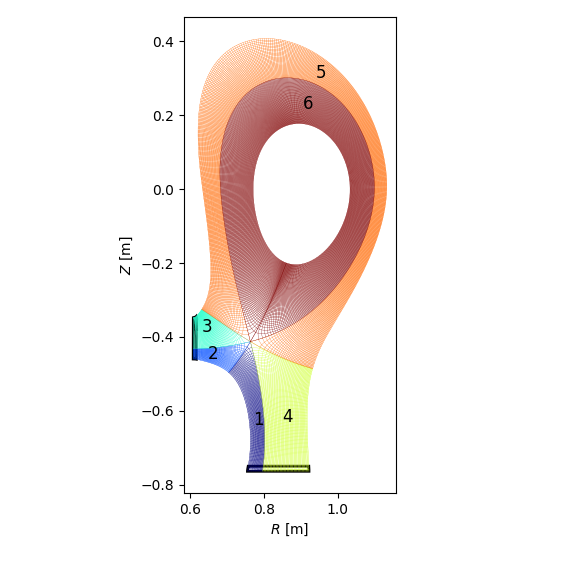
\includegraphics[width=1\textwidth]{schemes/TCVmesh.png}
		\subcaption{Typical mesh and zones decomposition}
		\label{fig:TCVmesh}
	\end{subfigure}
	\begin{subfigure}[c]{0.3\textwidth}
		\centering
		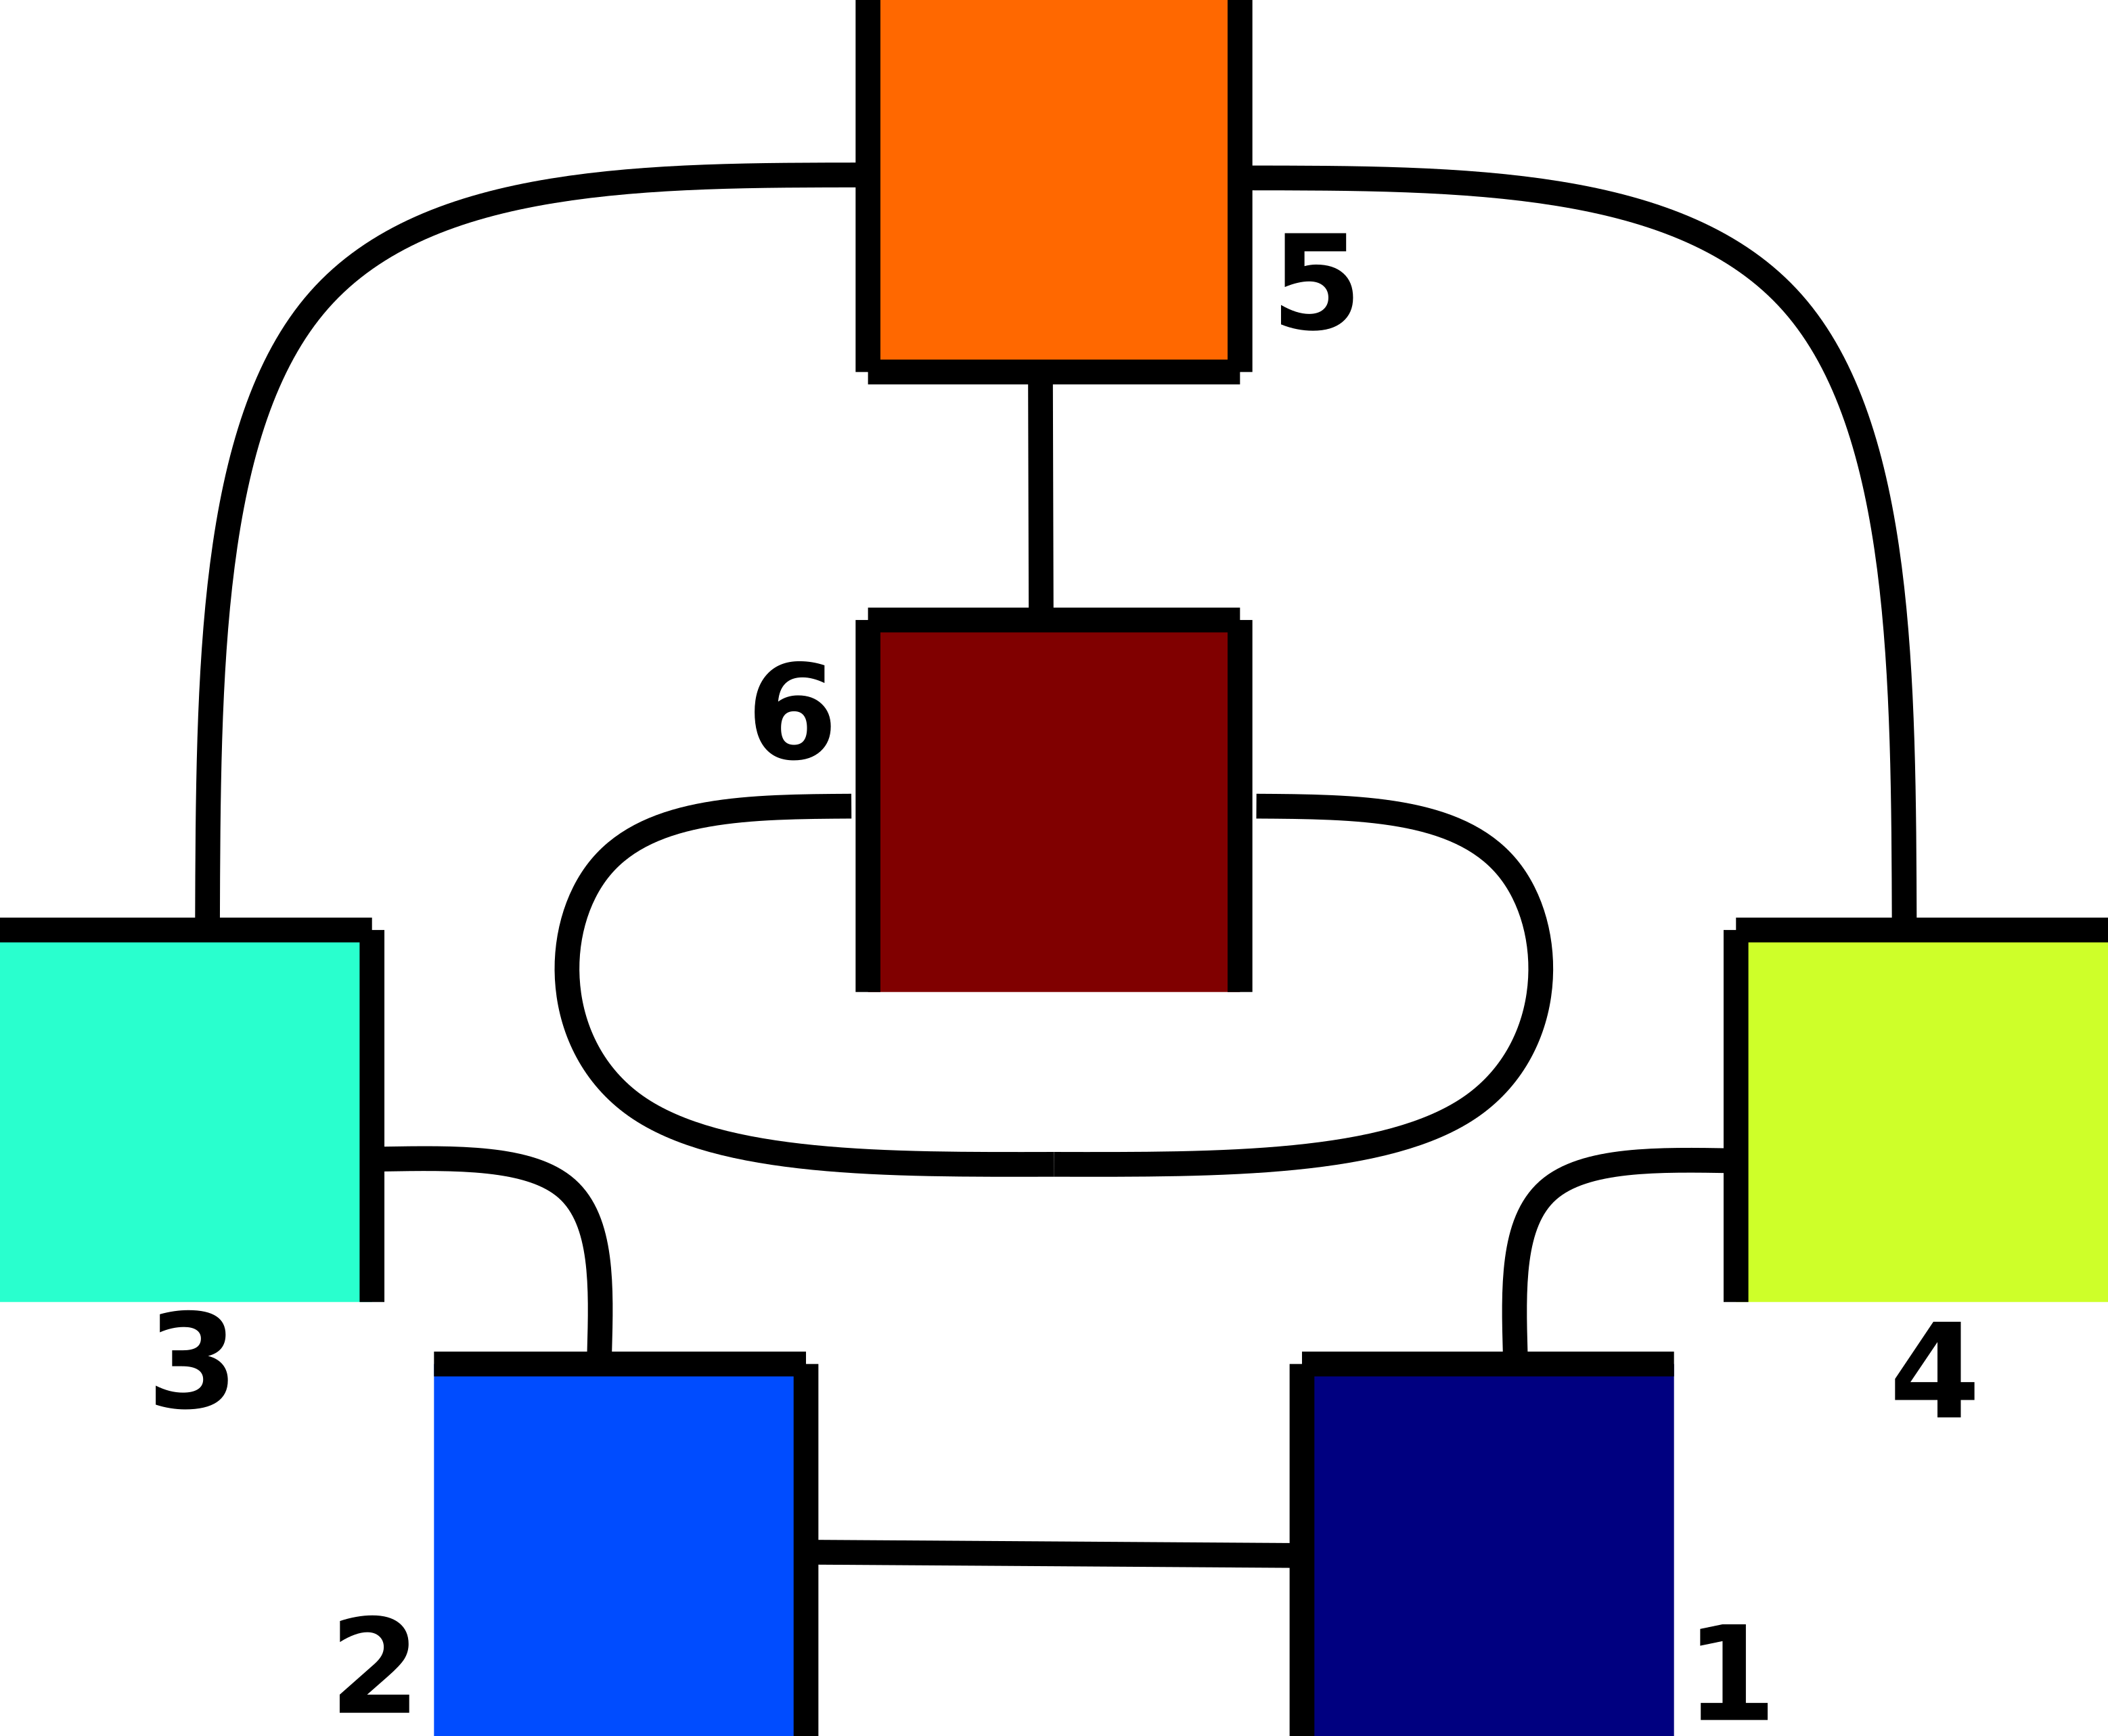
\includegraphics[width=1\textwidth]{schemes/TCV_domains.png}
		\subcaption{Connected zones in the domain decomposition}
		\label{fig:TCV_domains}
	\end{subfigure}
	
	\caption{ Example of typical mesh and domain decomposition mapping the real domain (a) to a Cartesian multiple zones domain (b). Each colored zone is isomorphic to a cube, the lines connecting the edges indicate the neighbours mapping. }
	\label{fig:TCVzoneDecomposition}
\end{figure}

\subsection{Curvilinear coordinates}
\label{ssec:MetricCurvilinearCoordinates}

The flux-surface-aligned discretization involves a curved grid in poloidal $\theta$ and toroidal $\varphi$ directions. To map the real geometry to the orthonormal grid on each subdomain, we require a metric transformation. The second chapter of the book by D’haeseleer et al \cite{CurvilinearGrids} describes well the numerical implications of curvilinear grids and serves as the basis of the present implementation. \\

Let $U=[u^\psi, u^\theta, u^\varphi]^T$ be the three parameters that describe every point in the domain $\Omega$ with respect to the curvilinear system of coordinates. On a torus, we can find an invertible transformation $R$ that maps each possible $U\in\Omega$ to a unique point in cartesian coordinates, thus: 

\begin{equation}
	\begin{bmatrix} x \\ y \\ z\end{bmatrix} = \mathbf{R}(u^\psi, u^\theta, u^\varphi)
\end{equation}

If we fix one parameter and allow the two remaining to vary freely, we obtain the so-called coordinate surface. Analogously if we fix two parameters, we obtain the coordinate curve associated to the free parameter and an accommodating choice for the scalar values $u^i$ is the curve length from an arbitrary reference point. At any point $P\in\Omega$, a local basis ${\mathbf{e}_\psi, \mathbf{e}_\theta, \mathbf{e}_\varphi}$ can be defined by the tangents to the respective coordinate curves crossing this point. Consequently, the basis vectors are easily expressed as:

\begin{align}
	\mathbf{e}_\psi =& \pdv{\mathbf{R}}{u^\psi} & \mathbf{e}_\theta =& \pdv{\mathbf{R}}{u^\theta} & \mathbf{e}_\varphi =& \pdv{\mathbf{R}}{u^\varphi}
\end{align}

The parameter choice of $u^i$ can be seen as the curve length and it might or might not be a unit length. The dimension index appears in subscript $\mathbf{e}_i$ to indicate that the basis vectors originate from a $u^i$ located below the fraction line. \\
An alternative basis can be defined from the gradients of the parameters $u^i$ which hence uses a superscript notation:  

\begin{align}
	\mathbf{e}^\psi = & \grad{u^\psi} & \mathbf{e}^\theta = & \grad{u^\theta} & \mathbf{e}^\varphi = & \grad{u^\varphi}
\end{align}

These basis vectors are orthogonal to the respective coordinate surfaces at the point $P$. It can be shown that both basis are reciprocal, thus:
$$ e^i\cdot e_j = \delta^i_j $$
where $\delta^i_j$ is the Kronecker delta. \\
This leads to the introduction of the covariant (linked to subscripts) and contravariant (linked to the superscripts) components of a vector. As it is known from linear algebra, any vector $\mathbf{v}$ can be expressed with respect to an arbitrary basis $\tilde{\mathbf{e}_i}$ as $\mathbf{v}=\tilde{v}_i\tilde{\mathbf{e}}_i$. For the two previously introduced basis, the respective components of $\mathbf{v}$ are given by: 

\begin{align}
	\text{Covariant components: }    & v_i = \mathbf{v}\cdot\mathbf{e}_i & \Rightarrow && \mathbf{v} = v_i\mathbf{e}^i \\
	\text{Contravariant components: }& v^i = \mathbf{v}\cdot\mathbf{e}^i & \Rightarrow && \mathbf{v} = v^i\mathbf{e}_i \\
\end{align}

It is common practice to call the representation of $\mathbf{v}$ using the co-/contravariant components the co-/contravariant vector of $\mathbf{v}$ albeit the co- and contravariant vectors both naturally describe the same vector $\mathbf{v}$. \\
Next, we introduce the metric coefficients $g_{ij} = \mathbf{e}_i\cdot \mathbf{e}_j$ and their reciprocal metric coefficients $g^{ij} = \mathbf{e}^i\cdot \mathbf{e}^j$. If available, they allow for an easy both-way conversion of contravariant to covariant vectors and consequently an easy change of basis. 

\begin{align}
	v_i =& g_{ij}v^j & \mathbf{e}_i =& g_{ij}\mathbf{e}^j \\
	v^i =& g^{ij}v_j & \mathbf{e}^i =& g^{ij}\mathbf{e}_j 
\end{align}

It may be noted that the matrices formed by the indices $i,j\in\{\theta,\psi,\varphi\}$ are each other's inverse matrix. \\



\section{The staggered mesh}

In order to benefit from the first-order parallel derivative that separates the $A_\parallel$ and $j_\parallel$ from the other plasma fields $\Phi$, $n_e$, and $T_e$ (Eqs. \ref{eq:MagneticPotential} and \ref{eq:VorticityEquation}), these two variables are defined on a toroidally $\varphi$ and poloidally $\theta$ staggered grid. They are calculated at cell edges in the parallel direction and can be directly matched to the fluxes entering and leaving the collocated cells. One of the major benefits is to minimize numerical diffusion and preserve turbulent structures, following findings in FVM simulations for fluid mechanics \cite{meier1999comparison}. In the radial $\psi$ direction, we keep the collocated position as the only parallel gradient in $\psi$ comes from the flutter term, which in nature is much smaller than the equilibrium field. If the mesh were also staggered in $\psi$, we would face strong numerical radial diffusion of parallel fluxes, defying the motivation of a staggered grid for $A_\parallel$ and $j_\parallel$. \newline



\subsection{Description and notation of the staggered grid}
The scalar variable $A_\parallel$ is the magnitude of the parallel magnetic vector potential that is a factor of the unit vector $\mathbf{b}$ in direction of the externally induced magnetic field lines. By construction of the domain, $\mathbf{b}$ has only components in $\varphi$ and $\theta$ directions. So far, all physical quantities are calculated on the collocated grid points at the domain cell centers. In the newly introduced equation on $A_\parallel$, the magnetic vector potential appears homogeneous to the potential, pressure and temperature gradients and the additional $A_\parallel$ term in the original equation states that the divergence of $A_\parallel$ accounts for the change in vorticity. Thus, $A_\parallel$ is always one spatial derivative away from the original quantities. As it is common in classical CFD simulation the velocity, $A_\parallel$ is not defined on cell centers but on a staggered grid on the cell edges in $\psi$-direction. Because the magnetic field lines do not evolve in radial direction and only parallel gradients contribute to $A_\parallel$, its grid is only staggered in  poloidal and toroidal directions. To distinguish quantities on both grids, the indexes $[i_\psi, i_\theta - \frac{1}{2},i_\varphi-\frac{1}{2}]$ describe discrete positions on the staggered grid. \\

\begin{figure}[H]
	\centering
	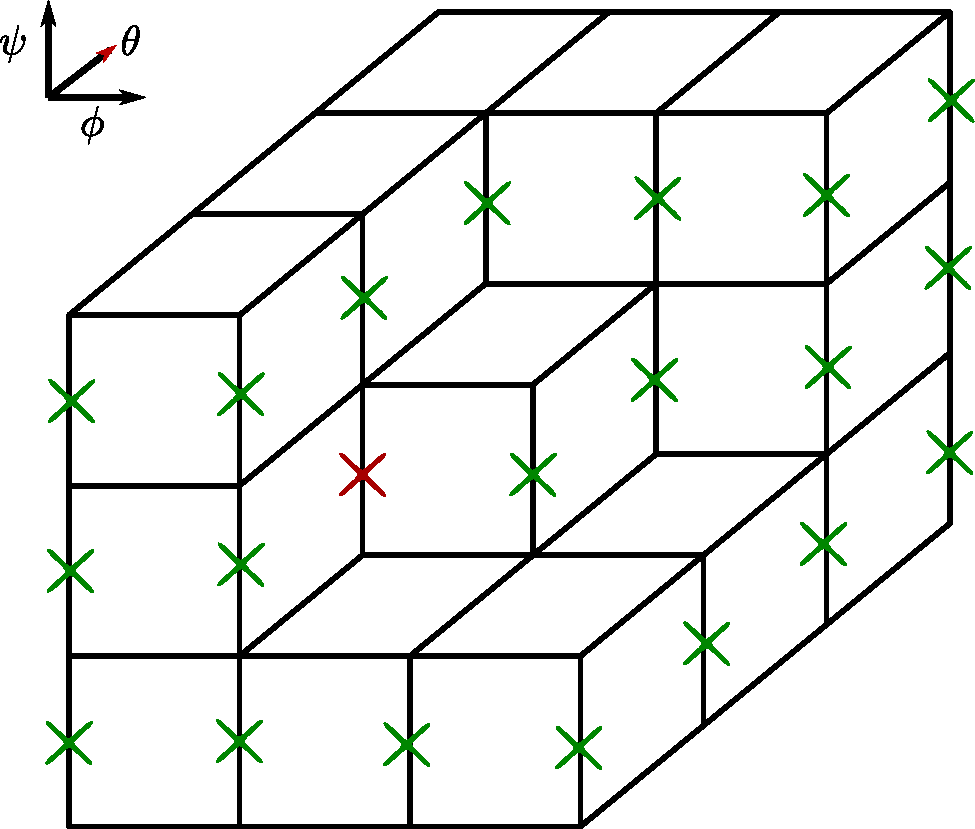
\includegraphics[width=0.4\textwidth]{schemes/StaggeredGrid.pdf}
	\caption{General view of the staggered grid points marked as crosses on top of the collocated cells. The red cross at the position $[i_\psi, i_\theta - \frac{1}{2}, i_\varphi-\frac{1}{2}]$ corresponds to the central cell with index $[i_\psi, i_\theta, i_\varphi]$}
	\label{fig:StaggeredGridOverview}
\end{figure}

In the following work, quantities evaluated at staggered grid points are indicated either by the superscript $stg$ or by a $-\frac{1}{2}$ shift in the index. This means that following notations are equivalent: 
\begin{align*}
	X^{stg}_{[i_\psi,i_\theta,i_\varphi]} &= X_{[i_\psi,i_\theta-\frac{1}{2},i_\varphi-\frac{1}{2}]} &\text{or}&& X^{stg}_{[i_\psi,i_\theta+1,i_\varphi]} &= X_{[i_\psi,i_\theta+\frac{1}{2},i_\varphi-\frac{1}{2}]}
\end{align*}



\subsection{Boundary cells}

Staggered quantities require a different treatment at the domain boundary. On the collocated mesh, cells are located either entirely in the plasma or in the physical wall. Staggered quantities in the boundary layer are thus always half a cell width away from the wall and boundary conditions are enforced accordingly. For the magnetic vector potential this holds for walls in $\psi$ direction but in $\varphi$ and $\theta$ directions, the staggered grid points are on the tokamak wall for the boundary cells with lowest index and one cell width away at the highest index. For consistency, accuracy and symmetry purposes, the staggered solvable domain shall be either extended by one row of cells at the upper index to include the wall in the solution or or reduced by one row at the lower end. In both cases, the number of collocated and staggered grid points do not match anymore and inhibit all eventual symmetry properties of the matrix in the dual-grid system (\ref{eq:vorticityEquation_electromagnetic_dedimensionalized_implicitEulerSystem}). $A_\parallel$ requires Dirichlet boundary conditions with the value 0 everywhere, thus the solution on the wall is already known and is not needed in the system. The parallel current $j_\parallel$ is fixed by the sheath current perpendicular to the wall, but is still needed for the parallel component tangential to the sheath. In Fig. \ref{fig:StaggeredGridBC}, the 

\begin{figure}[H]
	\centering
	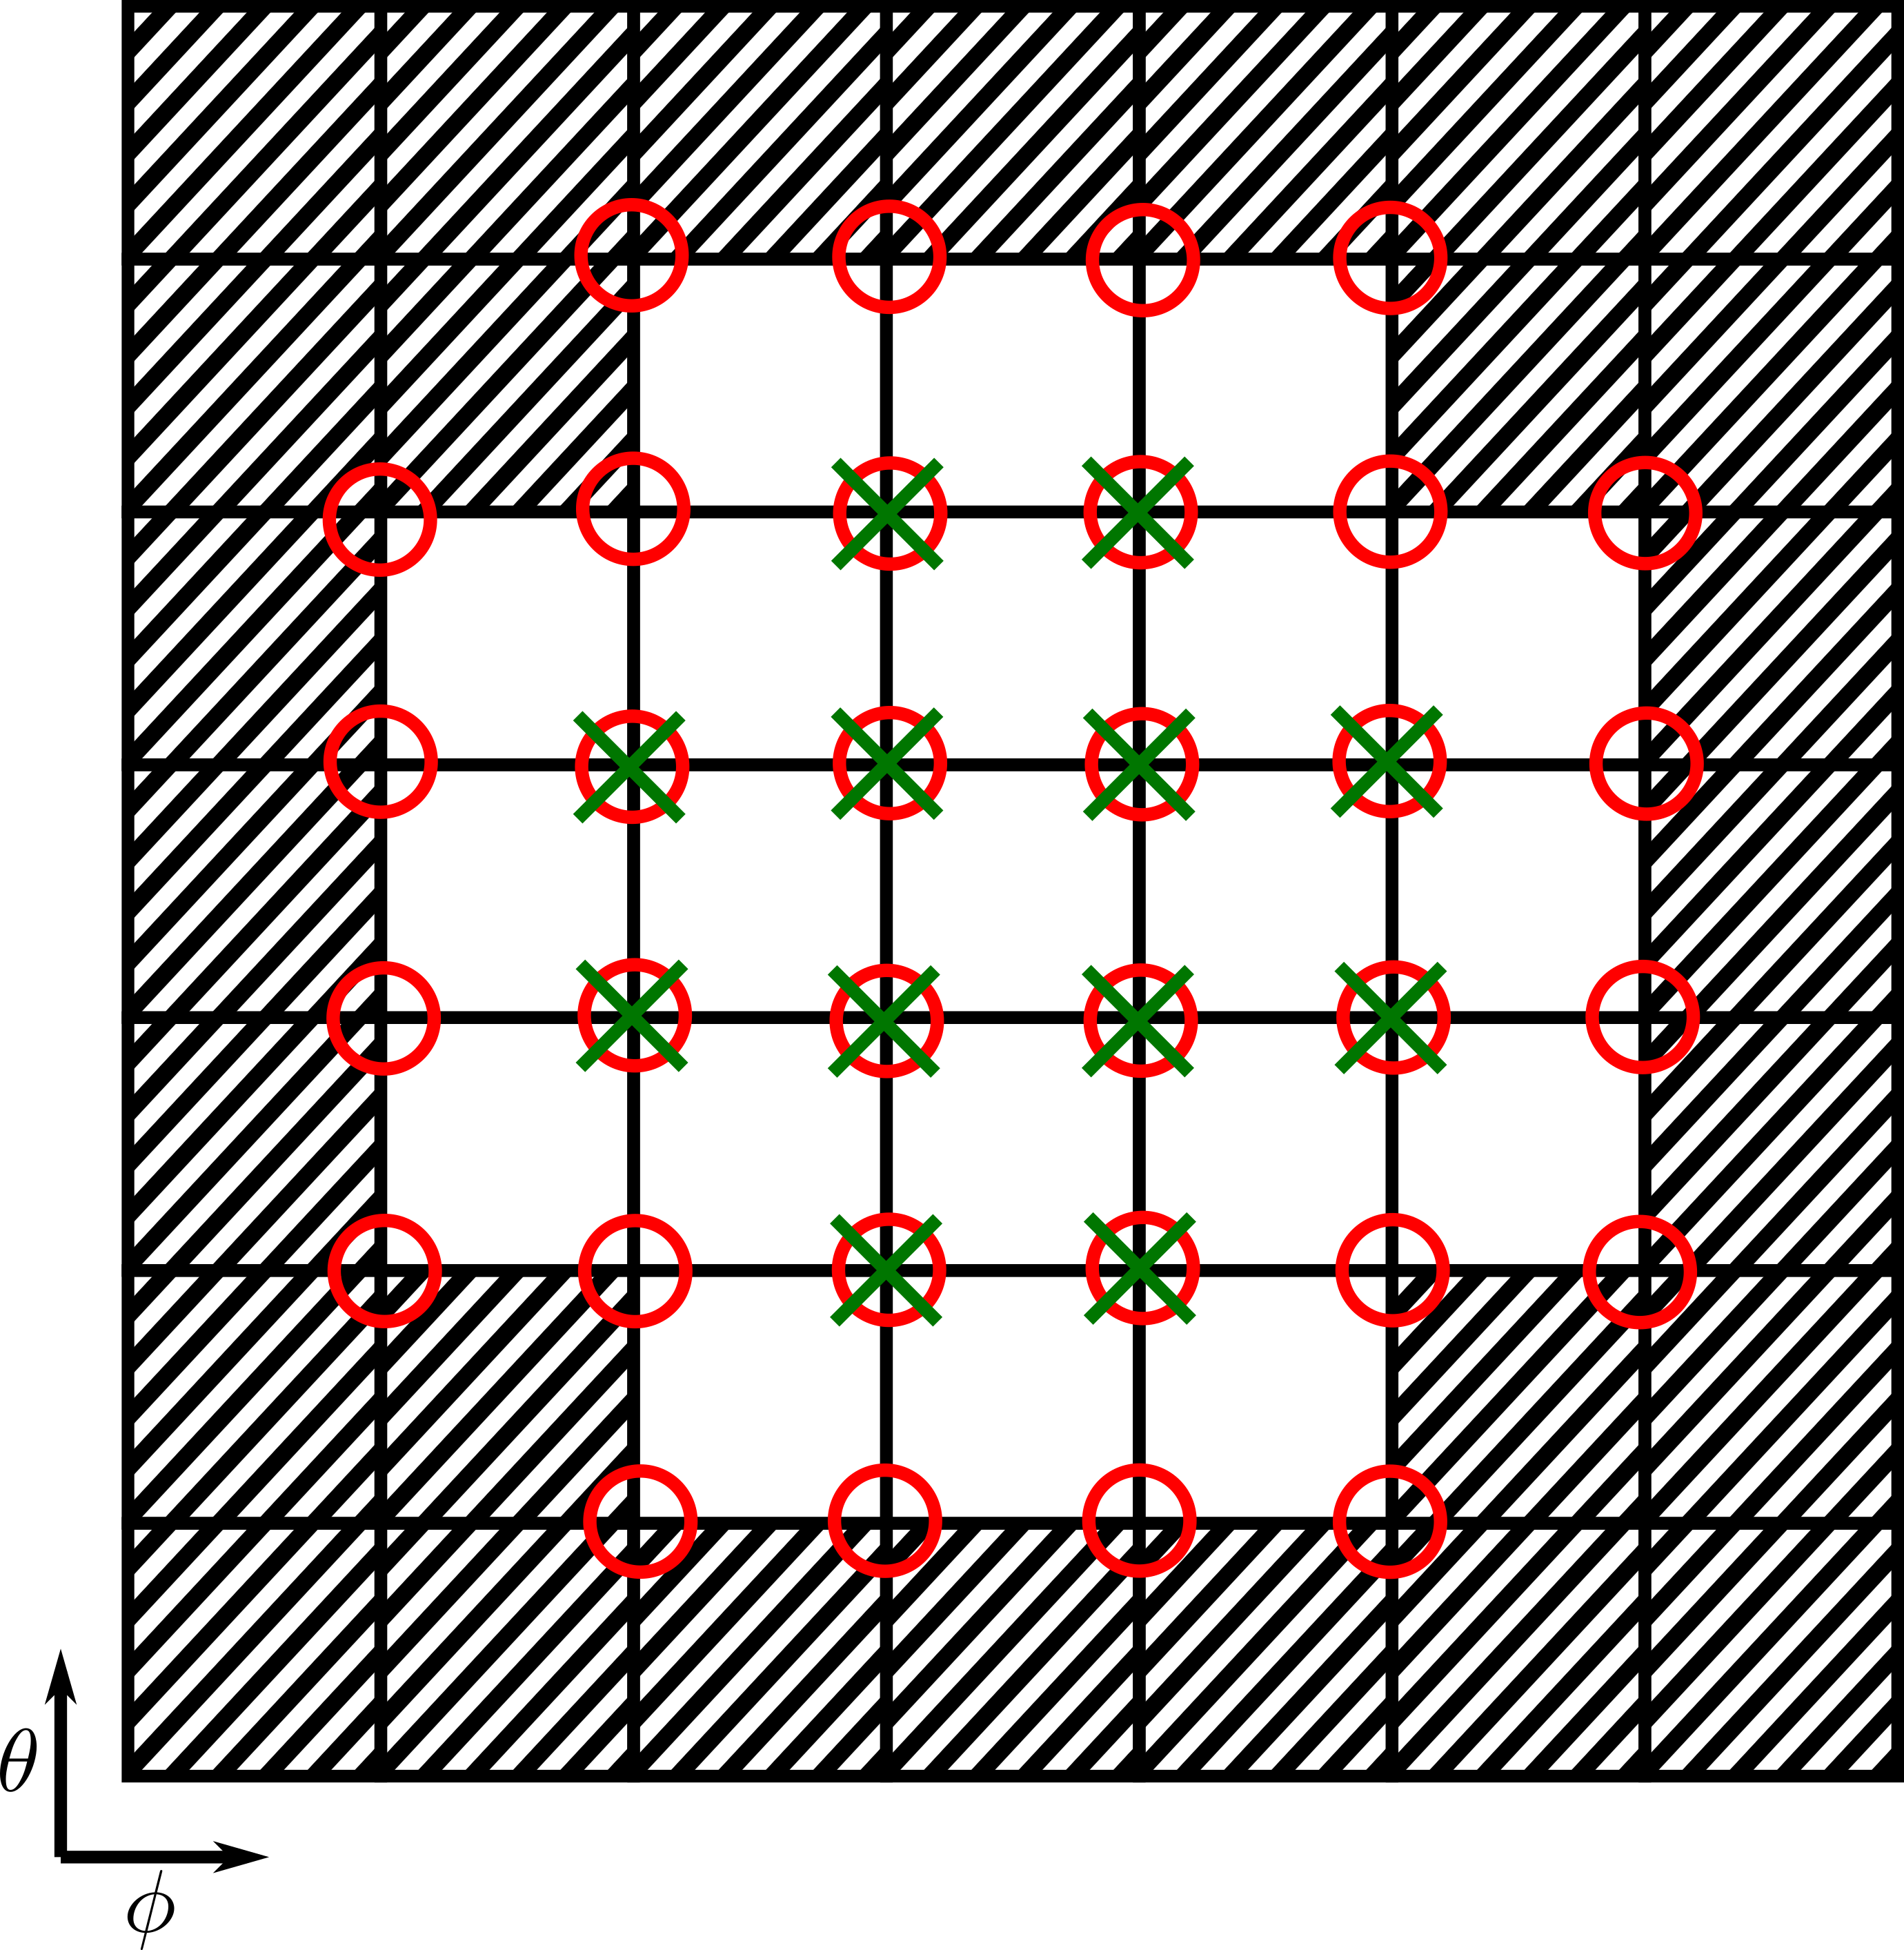
\includegraphics[width=0.6\textwidth]{schemes/staggeredGridBoundary.png}
	\caption{General view of the staggered grid points in the $\theta-\varphi$ plane. The field $A_\parallel$ is defined at the green crosses and $j_\parallel$ at the red circles. Crossed cells are boundary cells where the mask is $\chi = 1$. }
	\label{fig:StaggeredGridBC}
\end{figure}

To ensure a correct implementation of the system and the stencils that appear in it, a new mask describes which cells contain staggered grid points in the solvable domain. It is defined from the original collocated wall mask $\chi$ as:

\begin{align}
	\label{eq:def_chi_staggered}
	\chi^{A_\parallel}_{[i_\psi,i_\theta, i_\varphi]} &= 1 - 
	(1 - \chi_{[i_\psi,i_\theta  ,i_\varphi  ]})
	(1 - \chi_{[i_\psi,i_\theta-1,i_\varphi  ]})
	(1 - \chi_{[i_\psi,i_\theta  ,i_\varphi-1]})
	(1 - \chi_{[i_\psi,i_\theta-1,i_\varphi-1]}) \\
	\chi^{j_\parallel}_{[i_\psi,i_\theta, i_\varphi]} &= 
	\chi_{[i_\psi,i_\theta  ,i_\varphi  ]}
	\chi_{[i_\psi,i_\theta-1,i_\varphi  ]}
	\chi_{[i_\psi,i_\theta  ,i_\varphi-1]}
	\chi_{[i_\psi,i_\theta-1,i_\varphi-1]}
\end{align}

The value of $\chi^{A_\parallel}$ is therefore 1 if the staggered cell with index $[i_\psi,i_\varphi,i_\theta]$ overlaps with the wall and is 0 inside the solvable domain. Conversely, the mask $\chi^{j_\parallel}$ is 0 unless the entire cell lies in the wall. 


Let us discuss a bit further sheath boundary conditions for staggered fields, where $A_\parallel$ and $j_\parallel$ lie on the domain boundary. For collocated fields, we impose sheath fluxes from the Bohm-Chodura model (see Sec. \ref{sec:S3X_boundaryConditions}) on the first cell in the simulation domain. For the magnetic potential $A_\parallel$, the 0-Dirichlet condition is imposed in the concerned cell. For the parallel current $j_\parallel$, we add the sheath current $j_{\text{wall}}$ to any parallel currents tangential to the wall. Indeed, if the sheath boundary is in the $\theta$ direction, the $\varphi$ component of the parallel current remains unaffected and needs to be solved. 



\subsection{Staggered discrete operators}
As the parallel current $j_\parallel$ and the magnetic vector potential $A_\parallel$ are defined on a staggered grid, new stencil operators are needed to be compatible with the electric potential $\Phi$ defined on the collocated grid at the cell centers. 



\subsubsection{Parallel gradient}

To calculate the parallel current in Ohm's law, we require the parallel gradients of potential, density and electron temperature. The three fields are defined on the collocated grid, and the result of the operator shall lie on the staggered grid. 

\begin{equation}
	\left[\grad_{\parallel}X\right]^{stg}_{[i_\psi,i_\theta, i_\varphi]}
\end{equation}

Wave structure travel along the parallel direction, dominated by the equilibrium field $\mathbf{b}_{eq}$ in $\theta$ and $\varphi$-directions. Because of the high anisotropy given $B_{eq,p} \ll B_{eq,\varphi}$, this operator is prone to numerical dissipation if not properly implemented. Both directions are calculated in a common step

\begin{align}
	\left[\textbf{b}_{eq}\cdot\grad X \right]^{stg}_{[i_\psi,i_\theta, i_\varphi]} = \frac{1}{2}&\left(
	\left(+b^\theta_{stg} + b^\varphi_{stg}\right)X_{[i_\psi,i_\theta, i_\varphi]} + 
	\left(-b^\theta_{stg} + b^\varphi_{stg}\right)X_{[i_\psi,i_\theta-1, i_\varphi]} \right. \nonumber\\  &+ \left. 
	\left(+b^\theta_{stg} - b^\varphi_{stg}\right)X_{[i_\psi,i_\theta, i_\varphi-1]} + 
	\left(-b^\theta_{stg} - b^\varphi_{stg}\right)X_{[i_\psi,i_\theta-1, i_\varphi-1]}\right)
	\label{eq:Impl_GradParaStencil_FS}
\end{align}

This discrete operator involves four neighbors, as shown in Fig. \ref{fig:Impl_GradPara_ThetaPhi}. It is appreciated in the finite elements community for anisotropic wave propagation\cite{yee1966numerical,rubio2014finite, hasegawa2012staggered} for its good numerical properties and is used in the anisotropic heat diffusion problem in magnetized plasmas by Günter et al\cite{gunter2005}.


\begin{figure}[H]
	\centering
	\begin{subfigure}[t]{0.40\textwidth}
		\centering
		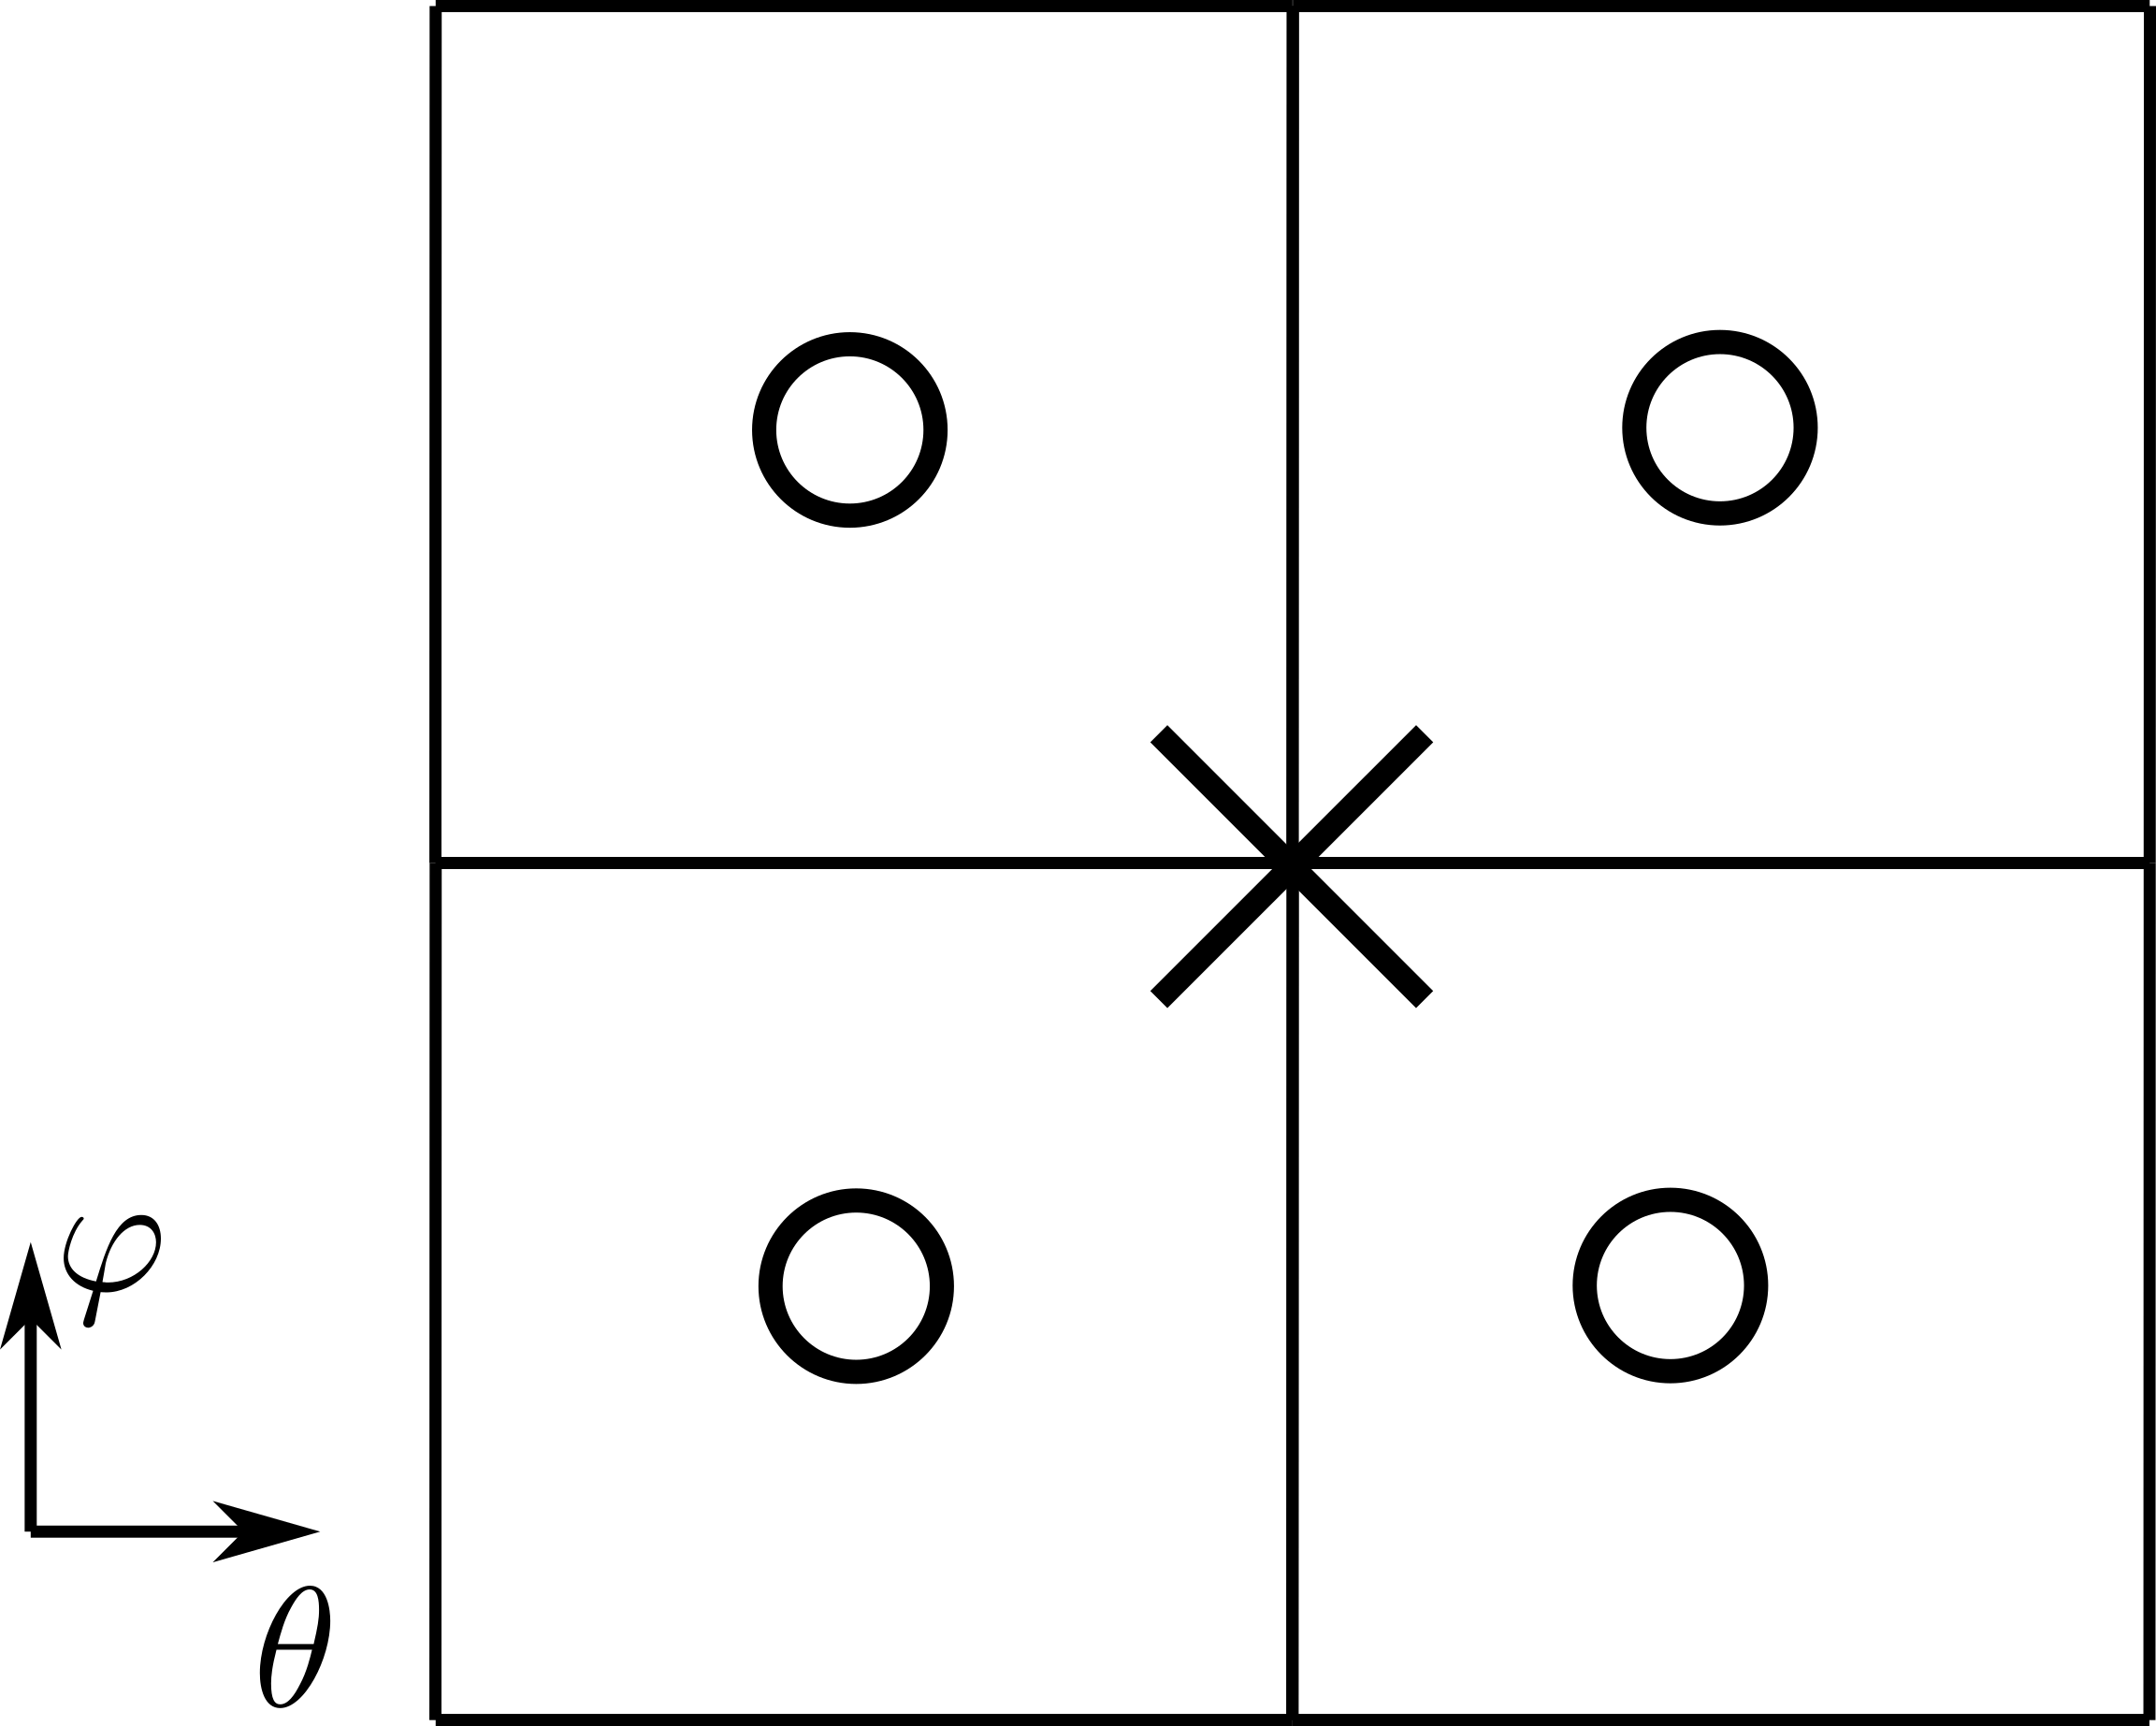
\includegraphics[height=40mm]{schemes/GradientStencil_ThetaPhi.png}
		\subcaption{Gradient along the equilibrium field}
		\label{fig:Impl_GradPara_ThetaPhi}
	\end{subfigure}
	\begin{subfigure}[t]{0.55\textwidth}
		\centering
		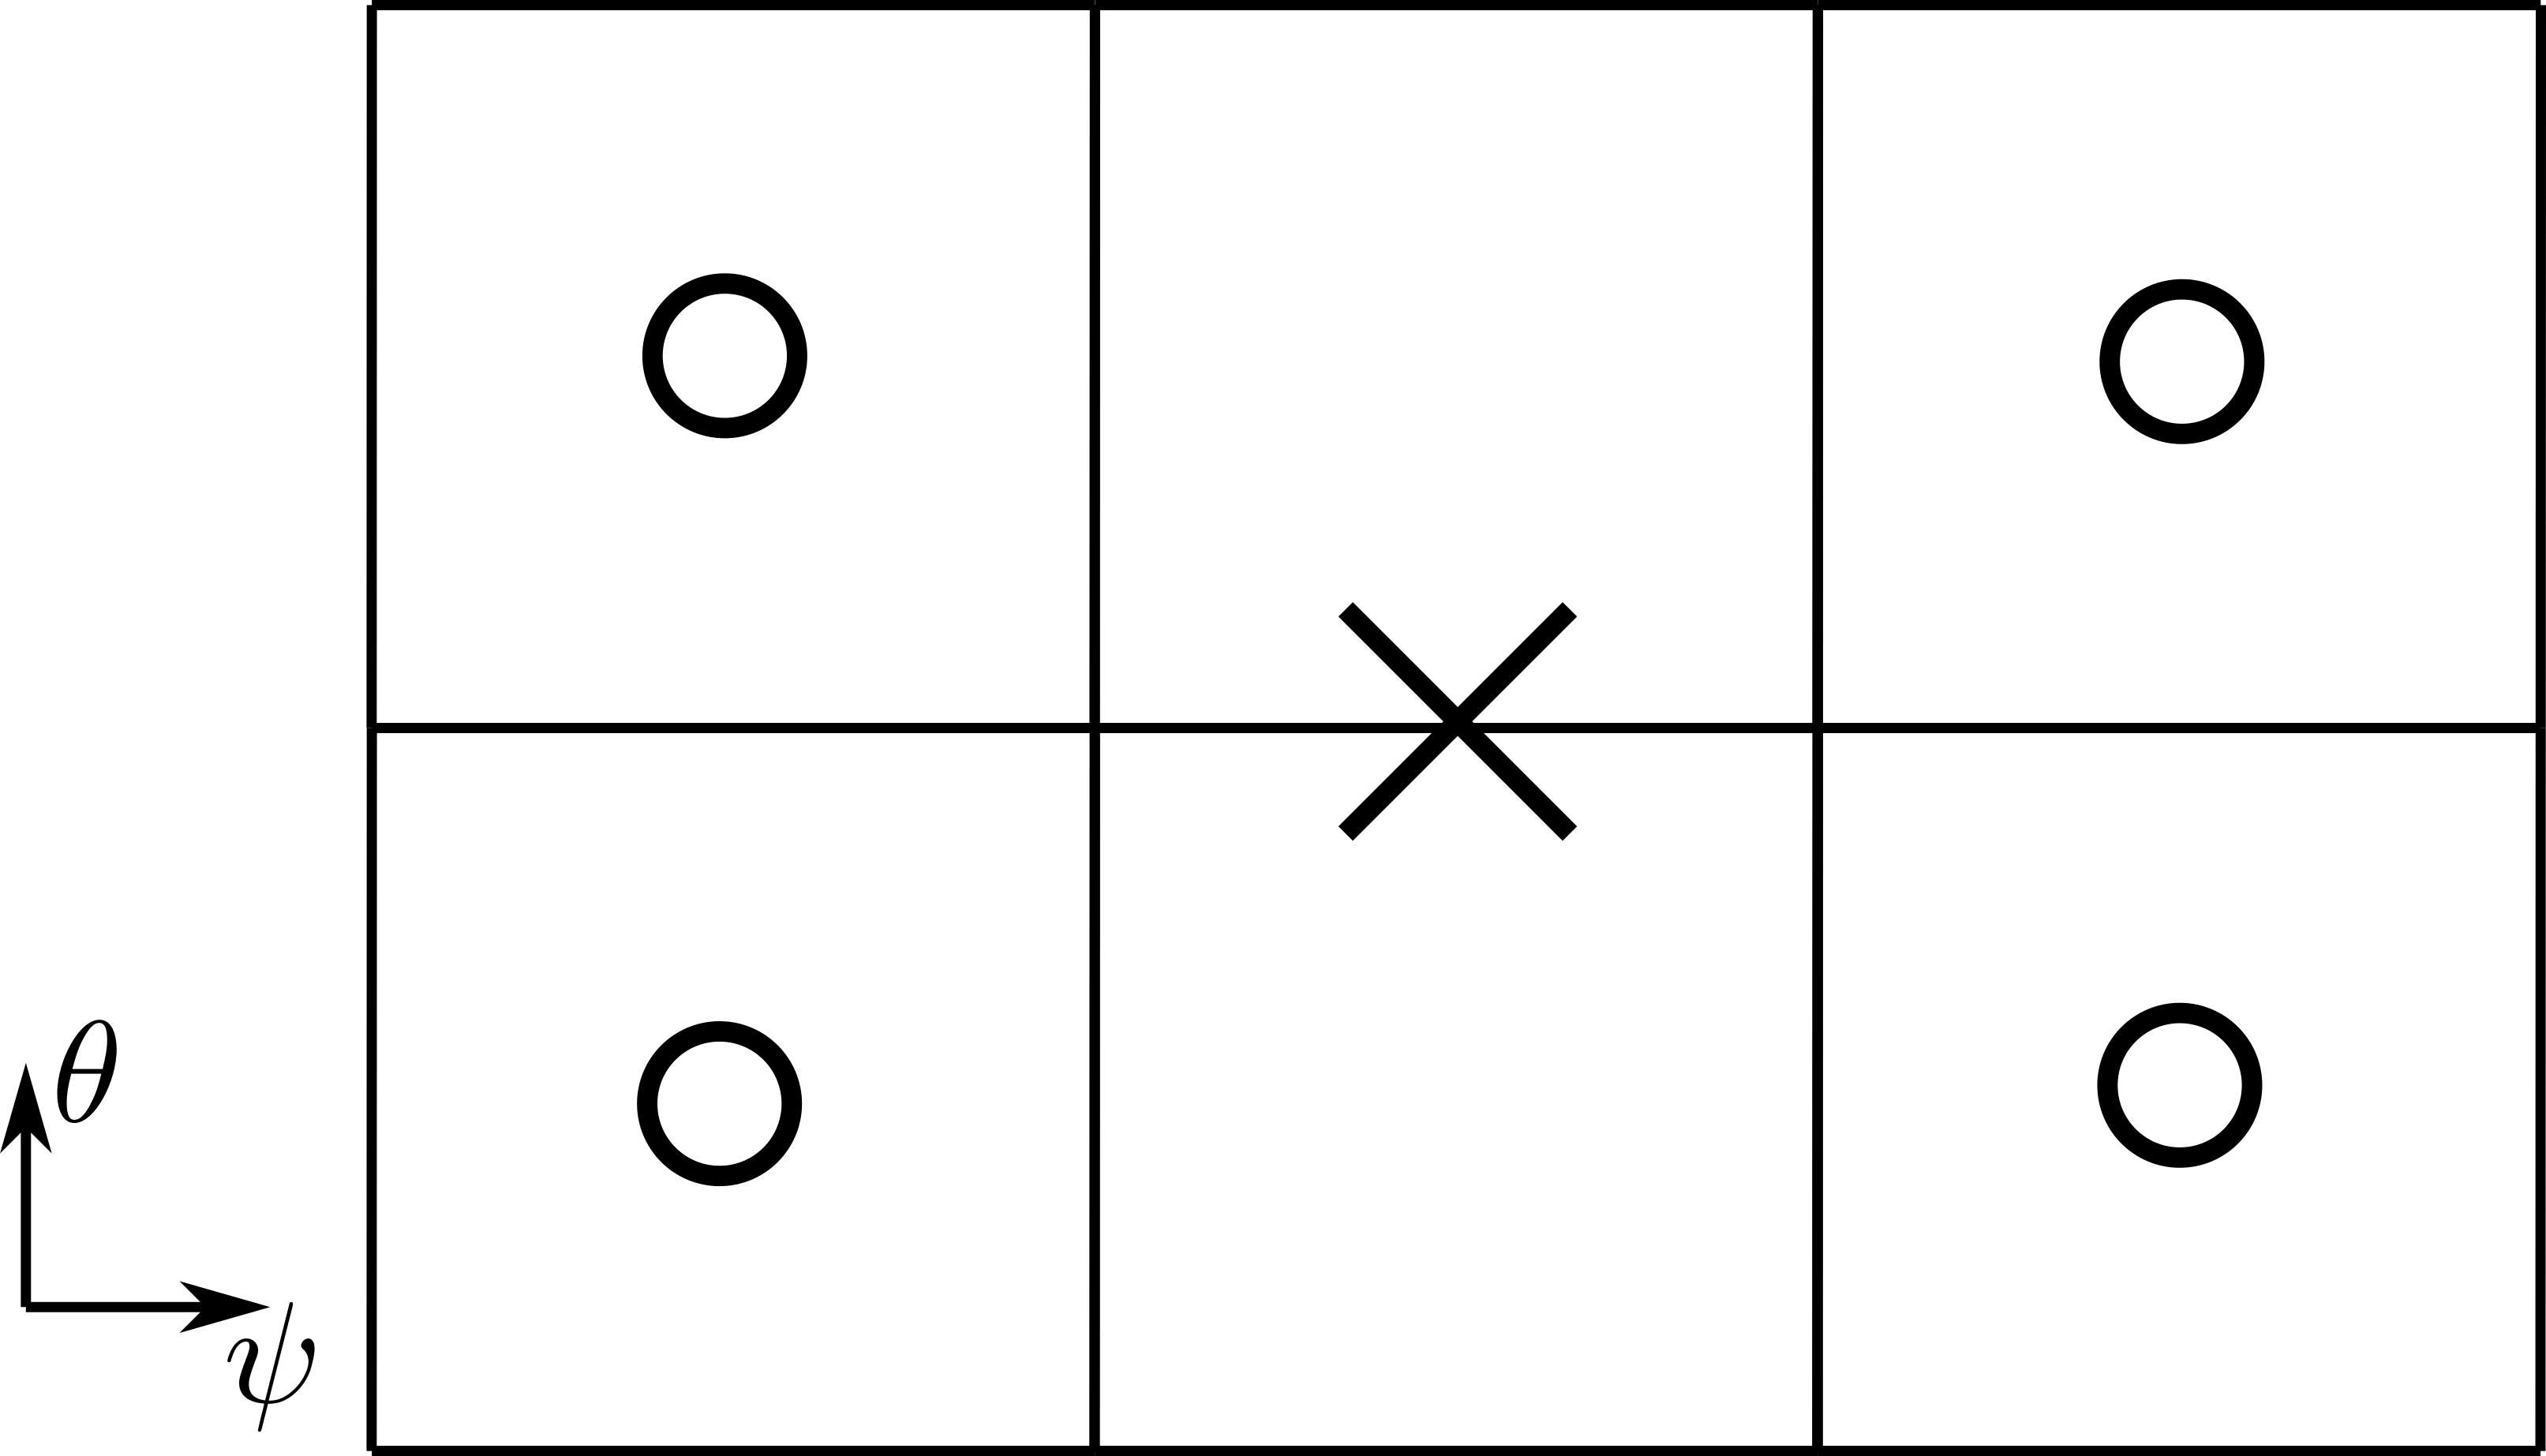
\includegraphics[height=40mm]{schemes/GradientStencil_PsiTheta.png}
		\subcaption{Gradient in radial direction}
		\label{fig:Impl_GradPara_PsiTheta}
	\end{subfigure}
	\caption{Neighbors involved to calculated staggered parallel gradients}
	\label{fig:Impl_GradPara}
\end{figure}

The gradient in radial direction, that comes from the magnetic flutter, is treated in a separate step. Because of the staggered grid configuration, that does not apply to the radial direction, the gradient requires 8 neighbors, of which four are shown in Fig. \ref{fig:Impl_GradPara_PsiTheta}, the other four being out of plane in the next poloidal plane.


\begin{align}
	\left[\tilde{\textbf{b}}\cdot\grad X \right]^{stg}_{[i_\psi,i_\theta, i_\varphi]} = \frac{1}{4}b^\psi_{stg}
	&\left( 
	  X_{[i_\psi+1,i_\theta, i_\varphi]} - X_{[i_\psi-1,i_\theta, i_\varphi]} 
	+  X_{[i_\psi+1,i_\theta, i_\varphi-1]} - X_{[i_\psi-1,i_\theta, i_\varphi-1]} \right. \nonumber \\ 
	&+ \left. X_{[i_\psi+1,i_\theta-1, i_\varphi]} - X_{[i_\psi-1,i_\theta-1, i_\varphi]} 
	+  X_{[i_\psi+1,i_\theta-1, i_\varphi-1]} - X_{[i_\psi-1,i_\theta-1, i_\varphi-1]}\right)
	\label{eq:Impl_GradParaStencil_flutter}
\end{align}



The poloidal and toroidal components of the magnetic flutuations are solved together with the equilibrium part in Eq. \ref{eq:Impl_GradParaStencil_FS}.


\subsubsection{Parallel divergence}

The divergence of $j_\parallel$ needs to be calculated at the collocated grid in the vorticity equation. It is the counterpart to the gradient operator above, and calculates the divergence on the collocated grid based on staggered fields. 

\begin{equation}
	\left[\grad\cdot X^{stg}\mathbf{b}\right]_{[i_\psi,i_\theta, i_\varphi]}
\end{equation}

In \autoref{eq:MetricDivergenceParallel}, the divergence of a parallel vector field has been introduced. We consider a collocated cell as in \autoref{fig:StaggeredGridOverview}. The divergence is then the sum of all in- and outgoing fluxes $\pdv{\left(J X b^i\right)}{u^i}$ across the six cell faces. 

\begin{equation}
	\label{eq:NumericalStaggeredDivergenceStencil}
	\left[\grad\cdot X^{stg}\mathbf{b}\right]_{[i_\psi,i_\theta, i_\varphi]} = \frac{1}{J_{[i_\psi,i_\theta, i_\varphi]}} \left(F_{[i_\psi,i_\theta, i_\varphi]}^{X,\psi}-F_{[i_\psi+1,i_\theta, i_\varphi]}^{X,\psi} + F_{[i_\psi,i_\theta, i_\varphi]}^{X,\theta}-F_{[i_\psi,i_\theta+1, i_\varphi]}^{X,\theta}+F_{[i_\psi,i_\theta, i_\varphi]}^{X,\varphi}-F_{[i_\psi,i_\theta, i_\varphi+1]}^{X,\varphi}\right)
\end{equation}

We want calculate these fluxes from the flux $F^{X,i} = JXb^i$ of the staggered field $X^{stg}$. As centered cell faces do not overlap with the staggered grid, we need to take the interpolate the fluxes calculated at the staggered mesh onto the cell face. For the equilibrium direction it involves two neighbors per flux (see Fig. \ref{fig:Impl_DivPara_ThetaPhi}). As an example, here are the fluxes written out for the incoming poloidal flux:

\begin{align*}
	F_{[i_\psi,i_\theta, i_\varphi]}^{X,\theta} &= \frac{1}{2}\left(F_{[i_\psi,i_\theta-\frac{1}{2}, i_\varphi-\frac{1}{2}]}^{X,\theta} + F_{[i_\psi,i_\theta-\frac{1}{2}, i_\varphi+\frac{1}{2}]}^{X,\theta} \right)
\end{align*}

In the radial direction, we need, again, the fluxes at eight neighboring staggered locations to calculate a flux on a single cell face. 

\begin{align*}
	F_{[i_\psi,i_\theta, i_\varphi]}^{X,\psi} = \frac{1}{8}&\left(
	F_{[i_\psi,i_\theta-\frac{1}{2}, i_\varphi-\frac{1}{2}]}^{X,\psi} + 
	F_{[i_\psi,i_\theta-\frac{1}{2}, i_\varphi+\frac{1}{2}]}^{X,\psi} +
	F_{[i_\psi,i_\theta+\frac{1}{2}, i_\varphi-\frac{1}{2}]}^{X,\psi} + 
	F_{[i_\psi,i_\theta+\frac{1}{2}, i_\varphi+\frac{1}{2}]}^{X,\psi} 
	\right. \nonumber \\ &+\left.
	F_{[i_\psi-1,i_\theta-\frac{1}{2}, i_\varphi-\frac{1}{2}]}^{X,\psi} + 
	F_{[i_\psi-1,i_\theta-\frac{1}{2}, i_\varphi+\frac{1}{2}]}^{X,\psi} + 
	F_{[i_\psi-1,i_\theta+\frac{1}{2}, i_\varphi-\frac{1}{2}]}^{X,\psi} + 
	F_{[i_\psi-1,i_\theta+\frac{1}{2}, i_\varphi+\frac{1}{2}]}^{X,\psi} 	
	\right)
\end{align*}

\begin{figure}[H]
	\centering
	\begin{subfigure}[t]{0.48\textwidth}
		\centering
		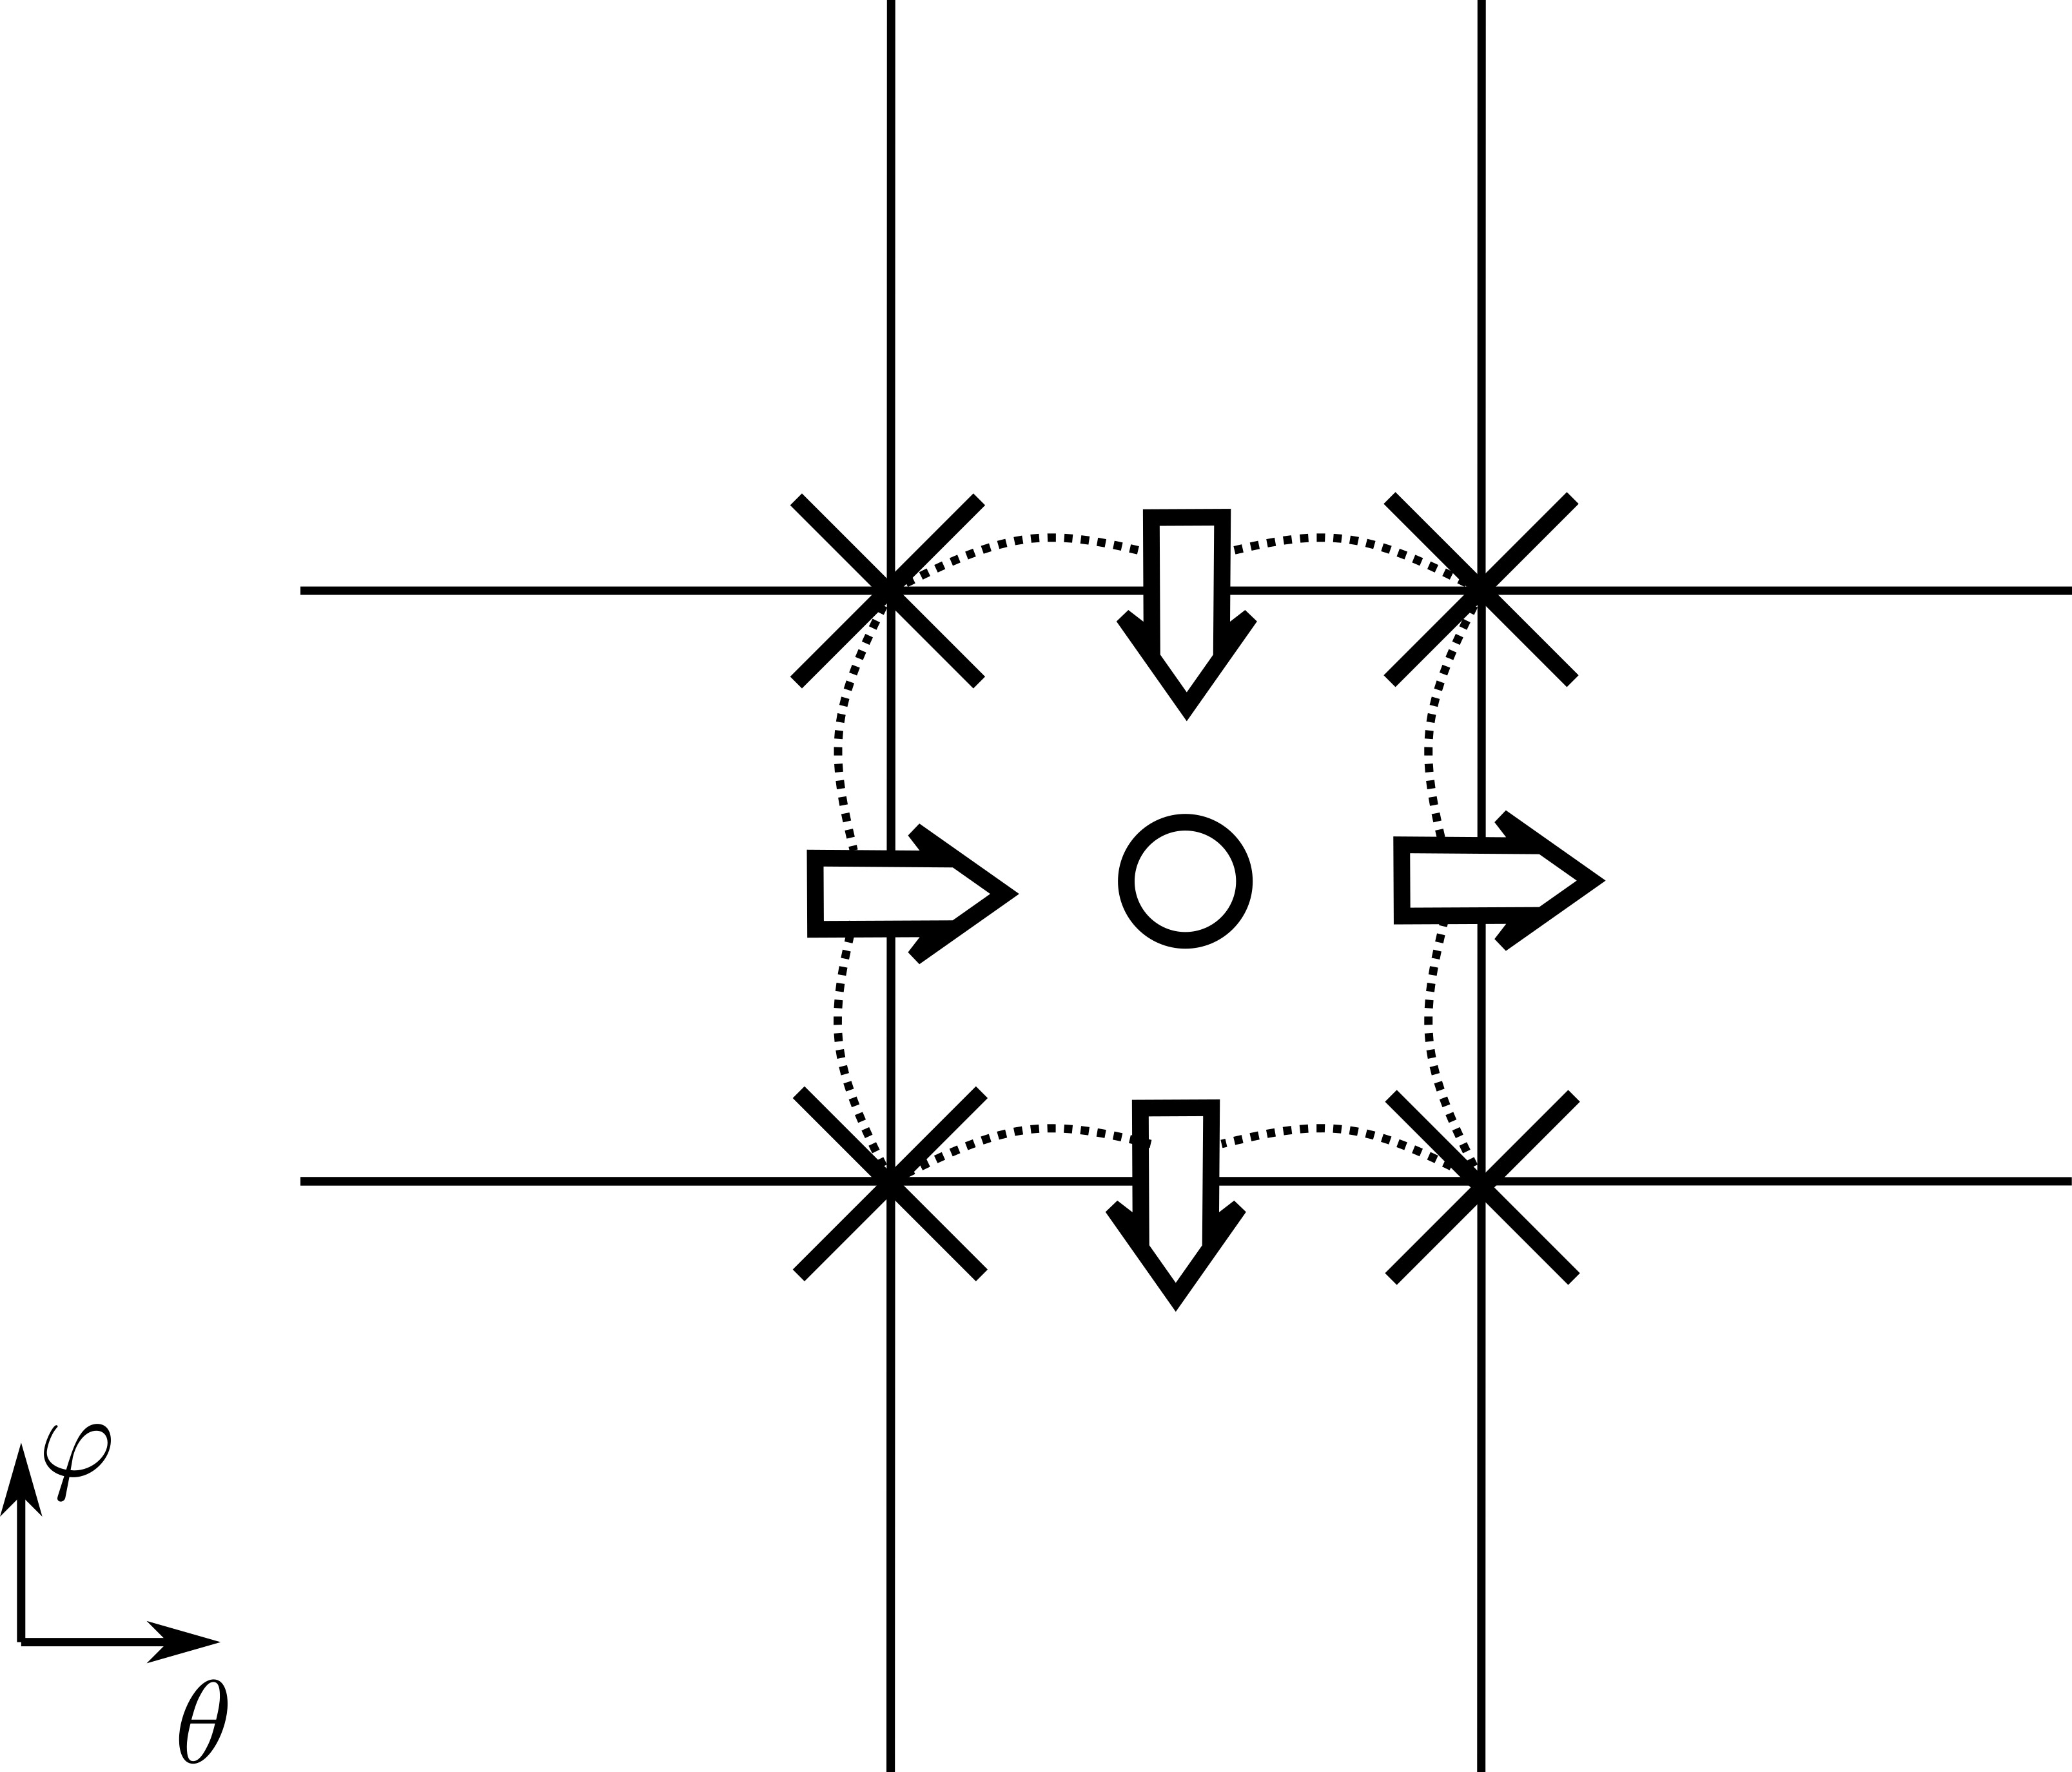
\includegraphics[height=60mm]{schemes/DivStencil_ThetaPhi.jpg}
		\subcaption{Divergence along the equilibrium field}
		\label{fig:Impl_DivPara_ThetaPhi}
	\end{subfigure}
	\begin{subfigure}[t]{0.48\textwidth}
		\centering
		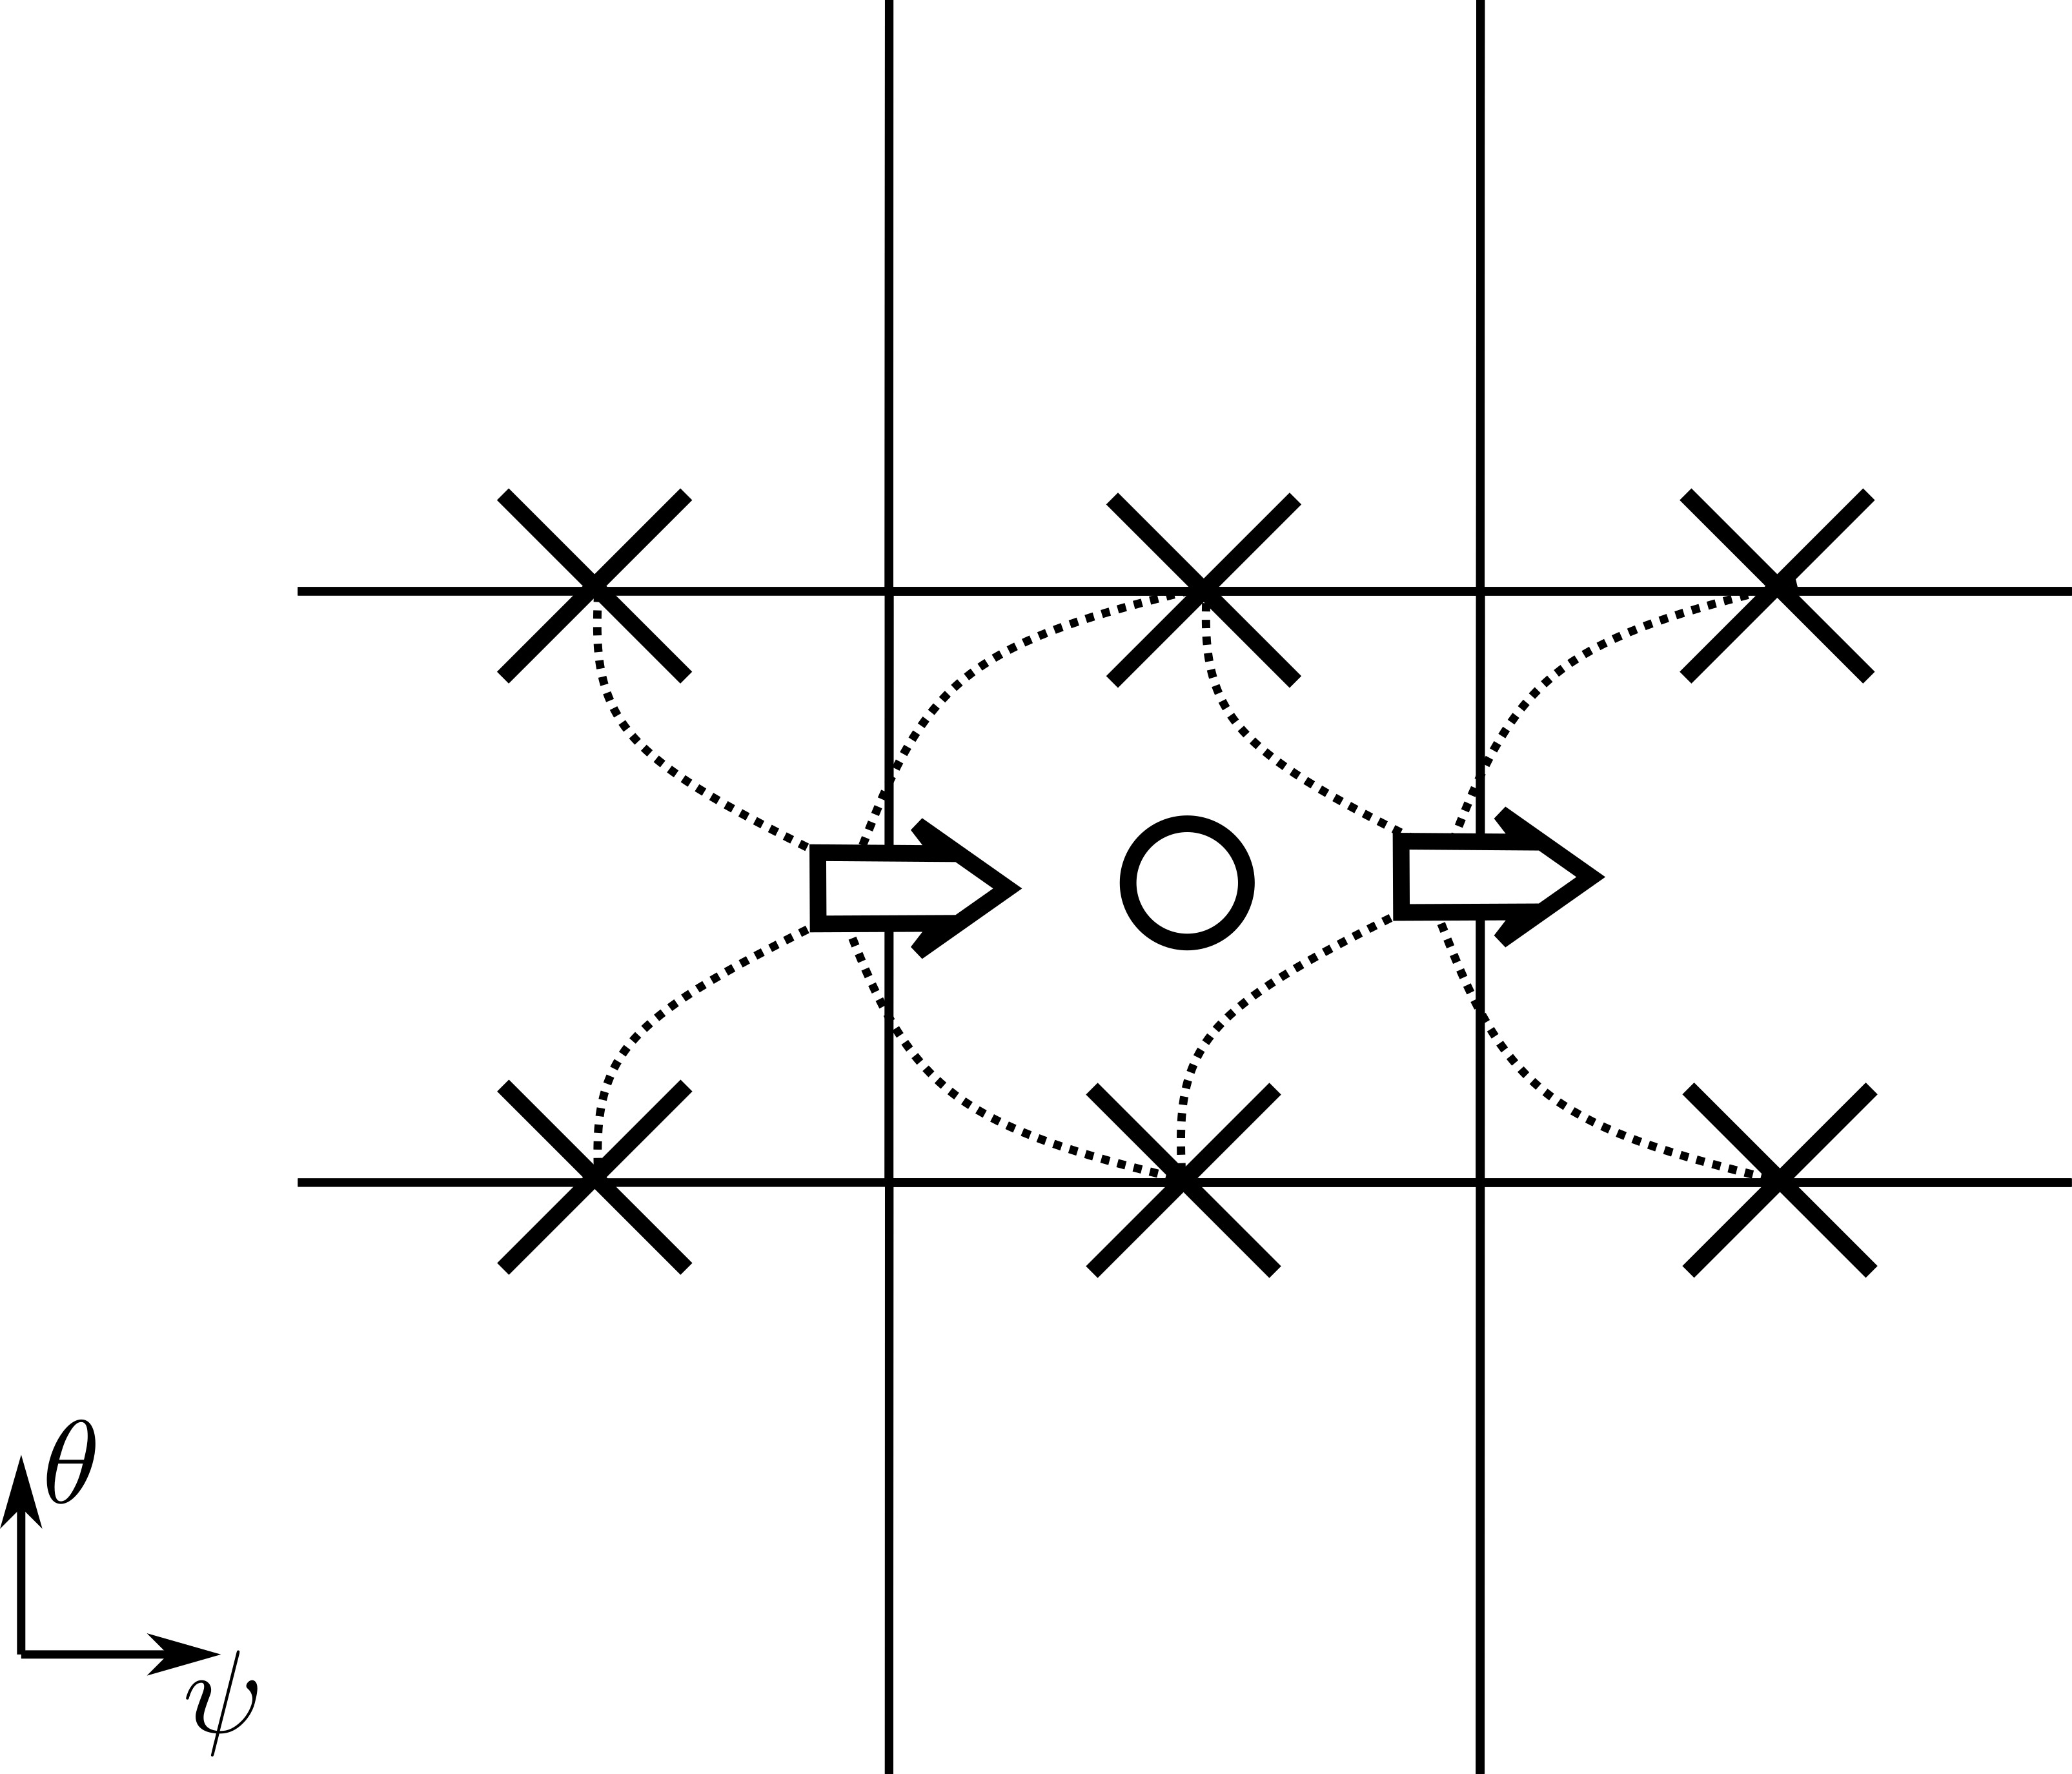
\includegraphics[height=60mm]{schemes/DivStencil_PsiTheta.jpg}
		\subcaption{Divergence in radial direction}
		\label{fig:Impl_DivPara_PsiTheta}
	\end{subfigure}
	\caption{Neighbors involved to calculated the parallel divergence. The arrows indicate the in- and outgoing fluxes that need to be calculated, and the dashed lines connect the arrows to the staggered points they require.}
	\label{fig:Impl_DivPara}
\end{figure}



\subsubsection{Perpendicular Laplacian}

Ampère's law requires the perpendicular Laplacian on the staggered grid to link $j_\parallel$ and $A_\parallel$, two staggered fields.

\begin{equation}
	\left[\grad\cdot\grad_{\perp}X^{stg}\right]^{stg}_{[i_\psi,i_\theta, i_\varphi]}
\end{equation}

Let us consider a staggered cell over the regular mesh, depicted in red in Fig. \ref{fig:StaggeredCell}. Since the Laplacian operator can be treated as a divergence of a gradient, the task . Each flux $F^{Y,i}$ is defined as the perpendicular gradient at the corresponding cell face, approximated with finite differences. The metric and diffusion coefficients $JD(g^{ij}-b^ib^j)$ are also required at the faces and we obtain them by taking their average on the closest collocated points. In poloidal and toroidal directions two collocated points shown in green in \autoref{fig:StaggeredFluxTheta} and \autoref{fig:StaggeredFluxPhi} are sufficient but in radial direction we need to consider eight points around the face to calculate the correct coefficients. \\

\begin{figure}[H]
	\centering
	\begin{subfigure}[b]{0.24\textwidth}
		\centering
		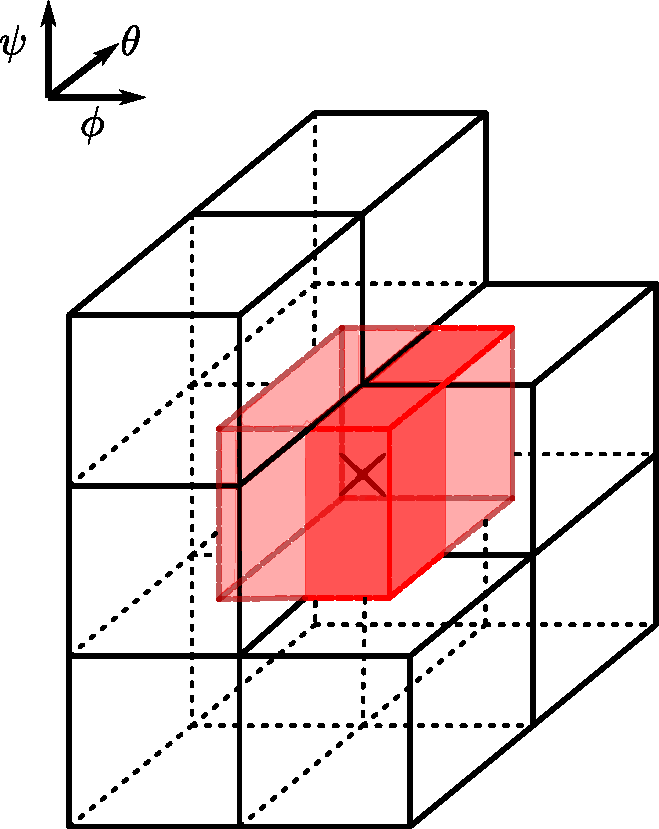
\includegraphics[width=1\textwidth]{schemes/BoundingBoxStaggeredPoint.pdf}
		\subcaption{Cell boundaries \\ for the staggered \\ grid point}
		\label{fig:StaggeredCell}
	\end{subfigure}
	\begin{subfigure}[b]{0.24\textwidth}
		\centering
		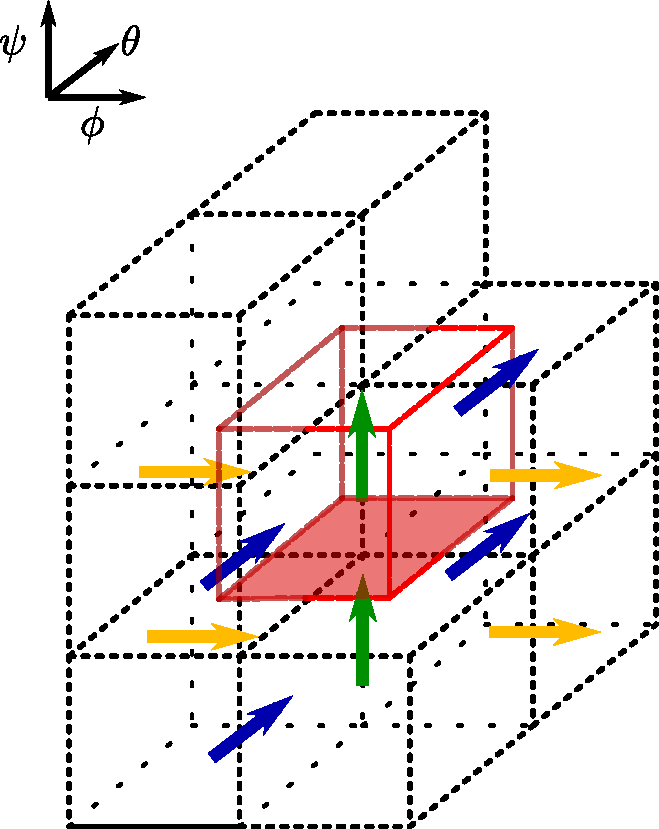
\includegraphics[width=1\textwidth]{schemes/BoundingBoxFluxPsiDiffPerp.pdf}
		\subcaption{Gradients \\ for fluxes \\ in $\psi$-direction} 
		\label{fig:StaggeredFluxPsi}
	\end{subfigure}
	\begin{subfigure}[b]{0.24\textwidth}
		\centering
		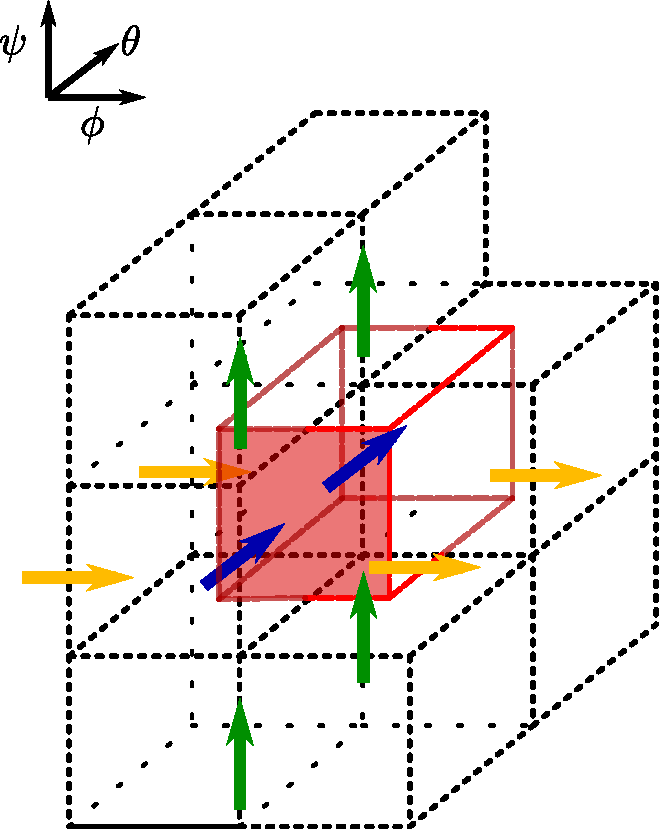
\includegraphics[width=1\textwidth]{schemes/BoundingBoxFluxThetaDiffPerp.pdf}
		\subcaption{Gradients \\ for fluxes \\ in $\theta$-direction} 
		\label{fig:StaggeredFluxTheta}
	\end{subfigure}
	\begin{subfigure}[b]{0.24\textwidth}
		\centering
		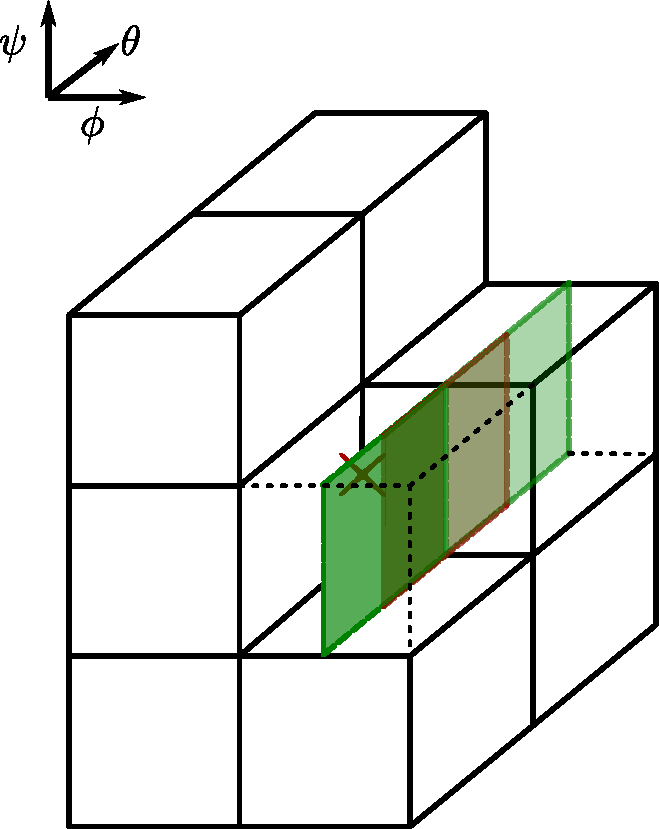
\includegraphics[width=1\textwidth]{schemes/BoundingBoxFluxPhiDiffPerp.pdf}
		\subcaption{Gradients \\ for fluxes \\ in $\varphi$-direction} 
		\label{fig:StaggeredFluxPhi}
	\end{subfigure}
	
	\caption{Depiction of the relevant cell faces to calculate fluxes of a staggered field at coordinate index $[i_\psi, i_\theta-\frac{1}{2}, i_\varphi-\frac{1}{2}]$}
	\label{fig:StaggeredPerpendicularLaplancianCellSurfaces}
\end{figure}





\subsection{Discretization around the X-point}
\label{ssec:DiscretizationXPt}

The staggered grid has direct implications on the estimation of fluxes around mesh singularities: while for regular fields, every cell around the X-point has well-defined neighbors (see Fig. \ref{fig:CenteredXpoint}), radial fluxes in and out of staggered cells directly cross the X-point (see Fig. \ref{fig:StaggeredXpoint}). They affect the perpendicular Laplacian operator on $A_\parallel$ in Ampere's law (Eq. \ref{eq:MagneticPotential}), advection on $j_\parallel$ in Eq. \ref{eq:advectionJpara}, and the anomalous perpendicular diffusion $\mathcal{D}_\perp$. To cope with the ill-defined cell faces, fluxes across the X-point are forced to 0 by Neumann-like boundary conditions. Neighbors of the involved cells must be defined separately from the regular cells with the same index. \newline

\begin{figure}[H]
	\centering
	\begin{subfigure}[t]{0.39\textwidth}
		\centering
		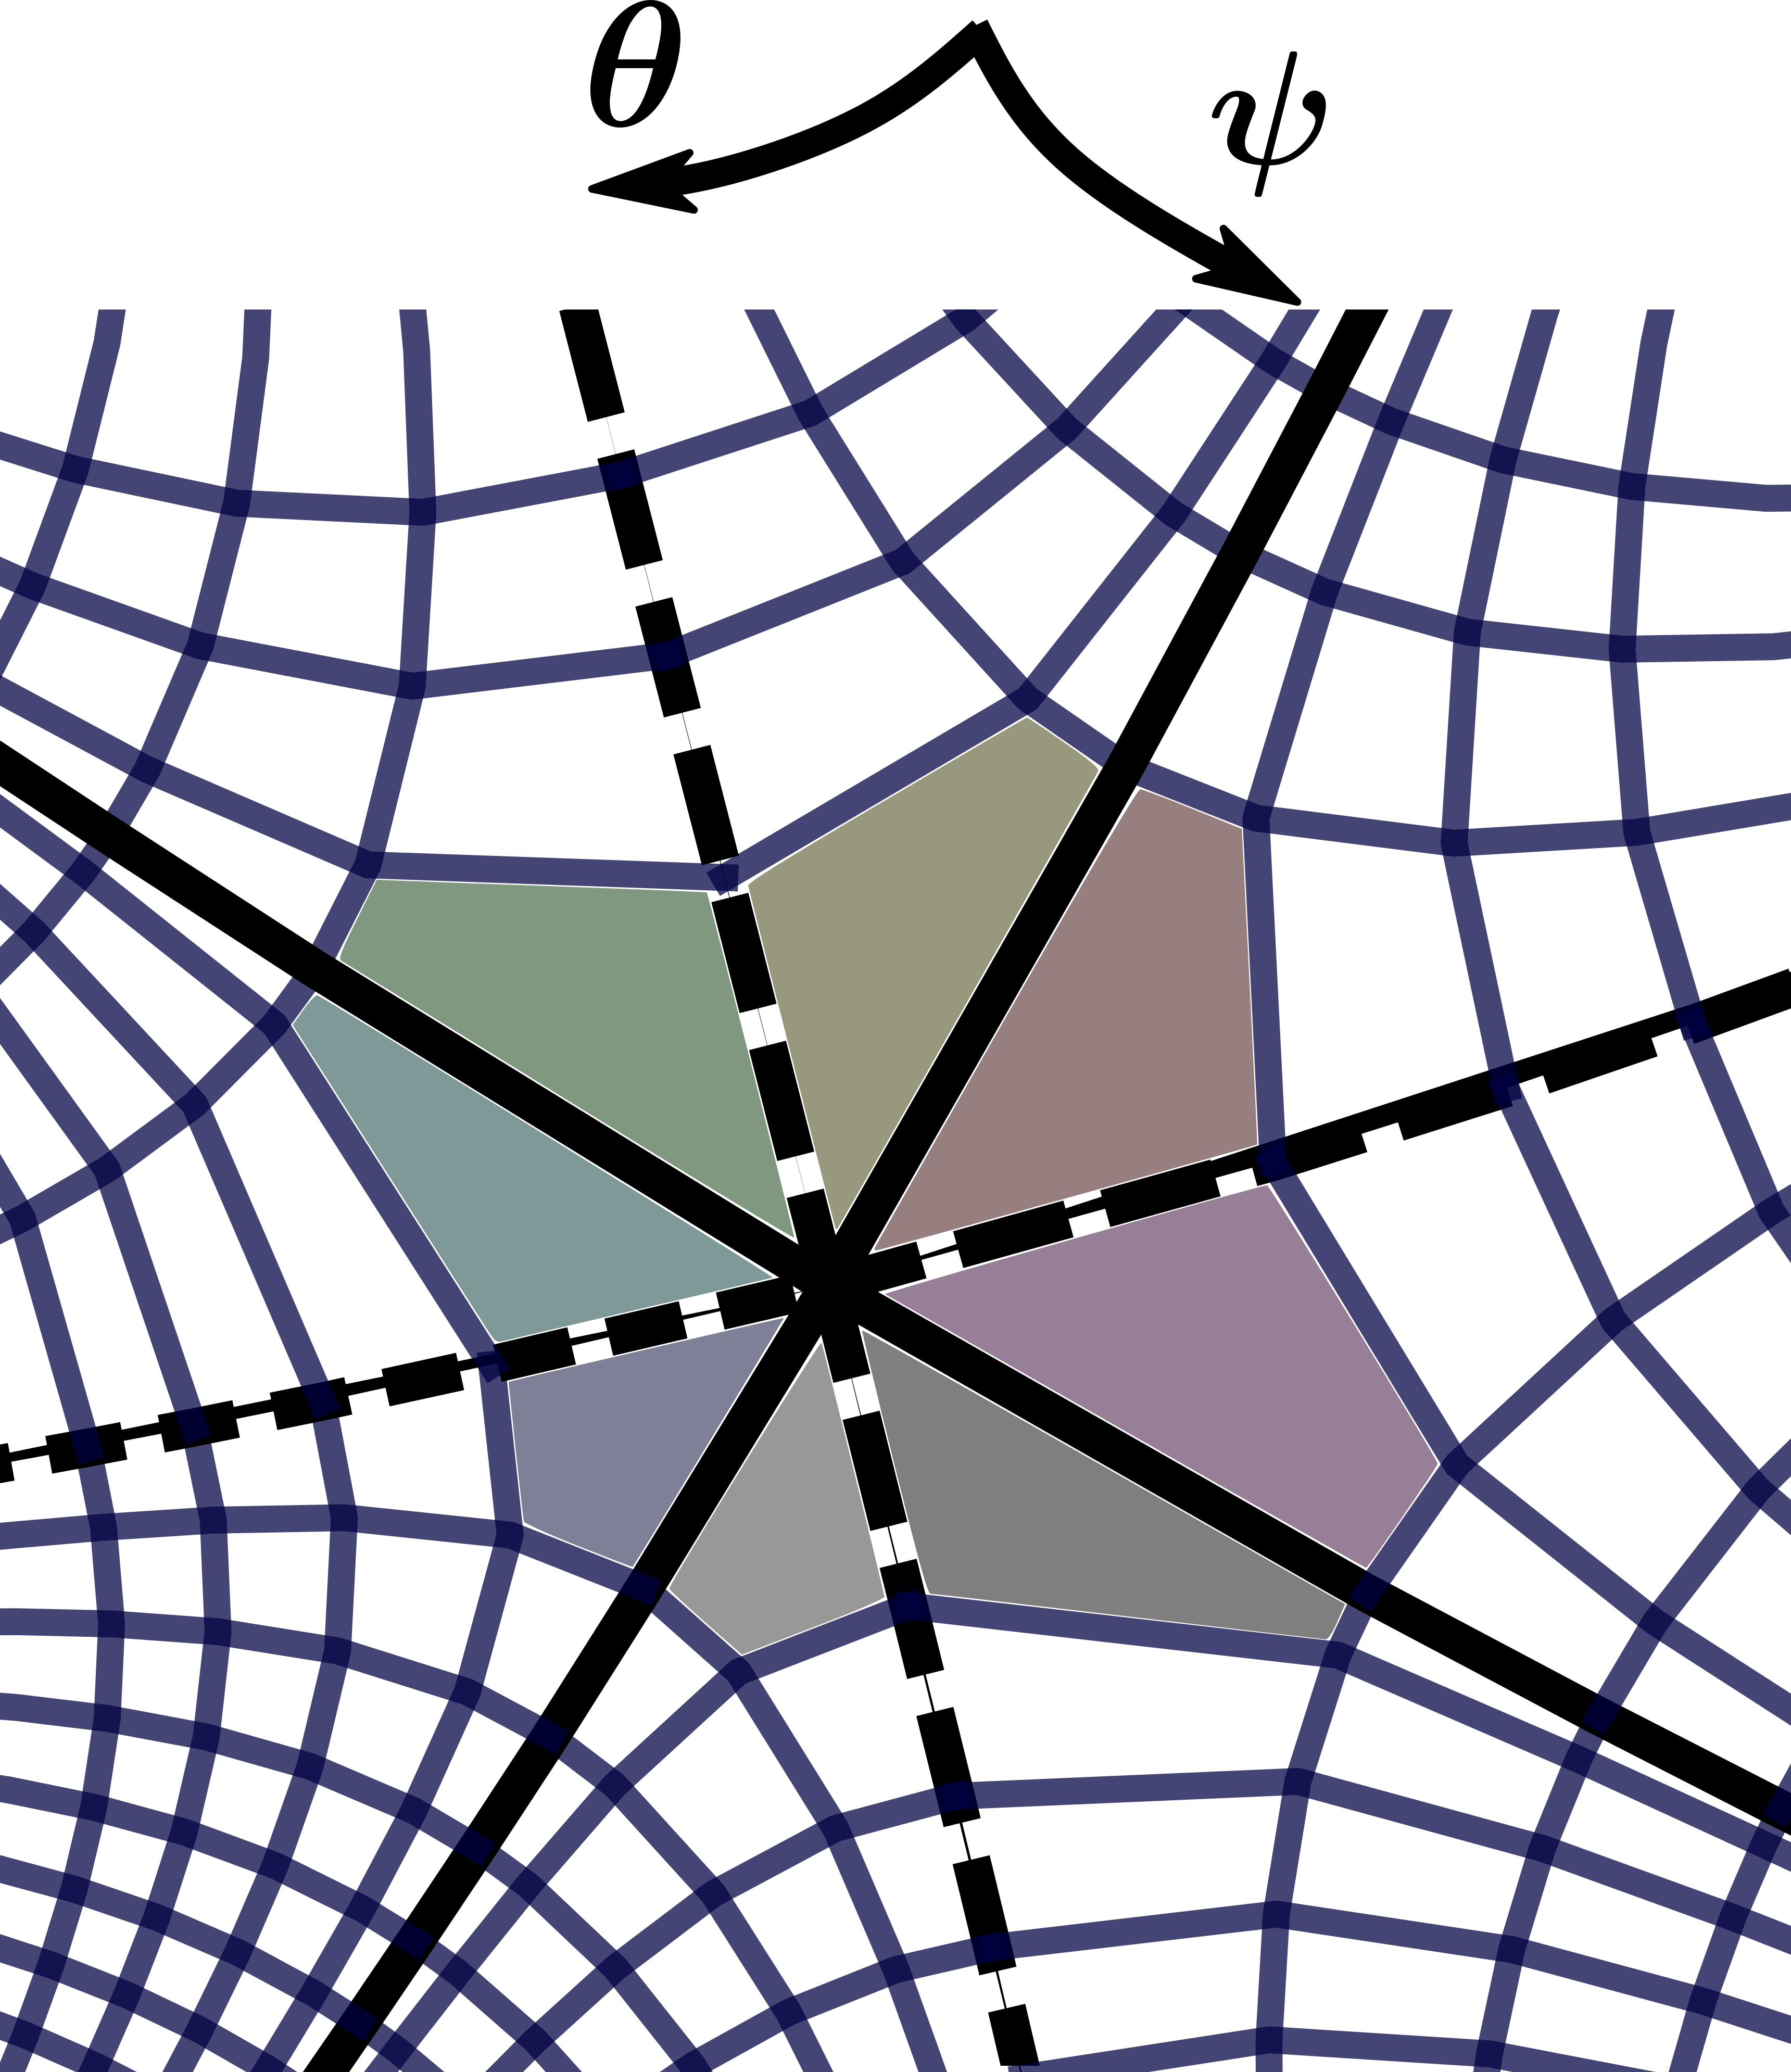
\includegraphics[width=1\textwidth]{schemes/XpointCentered.png}
		\subcaption{View of collocated cells}
		\label{fig:CenteredXpoint}
	\end{subfigure}
	\begin{subfigure}[t]{0.39\textwidth}
		\centering
		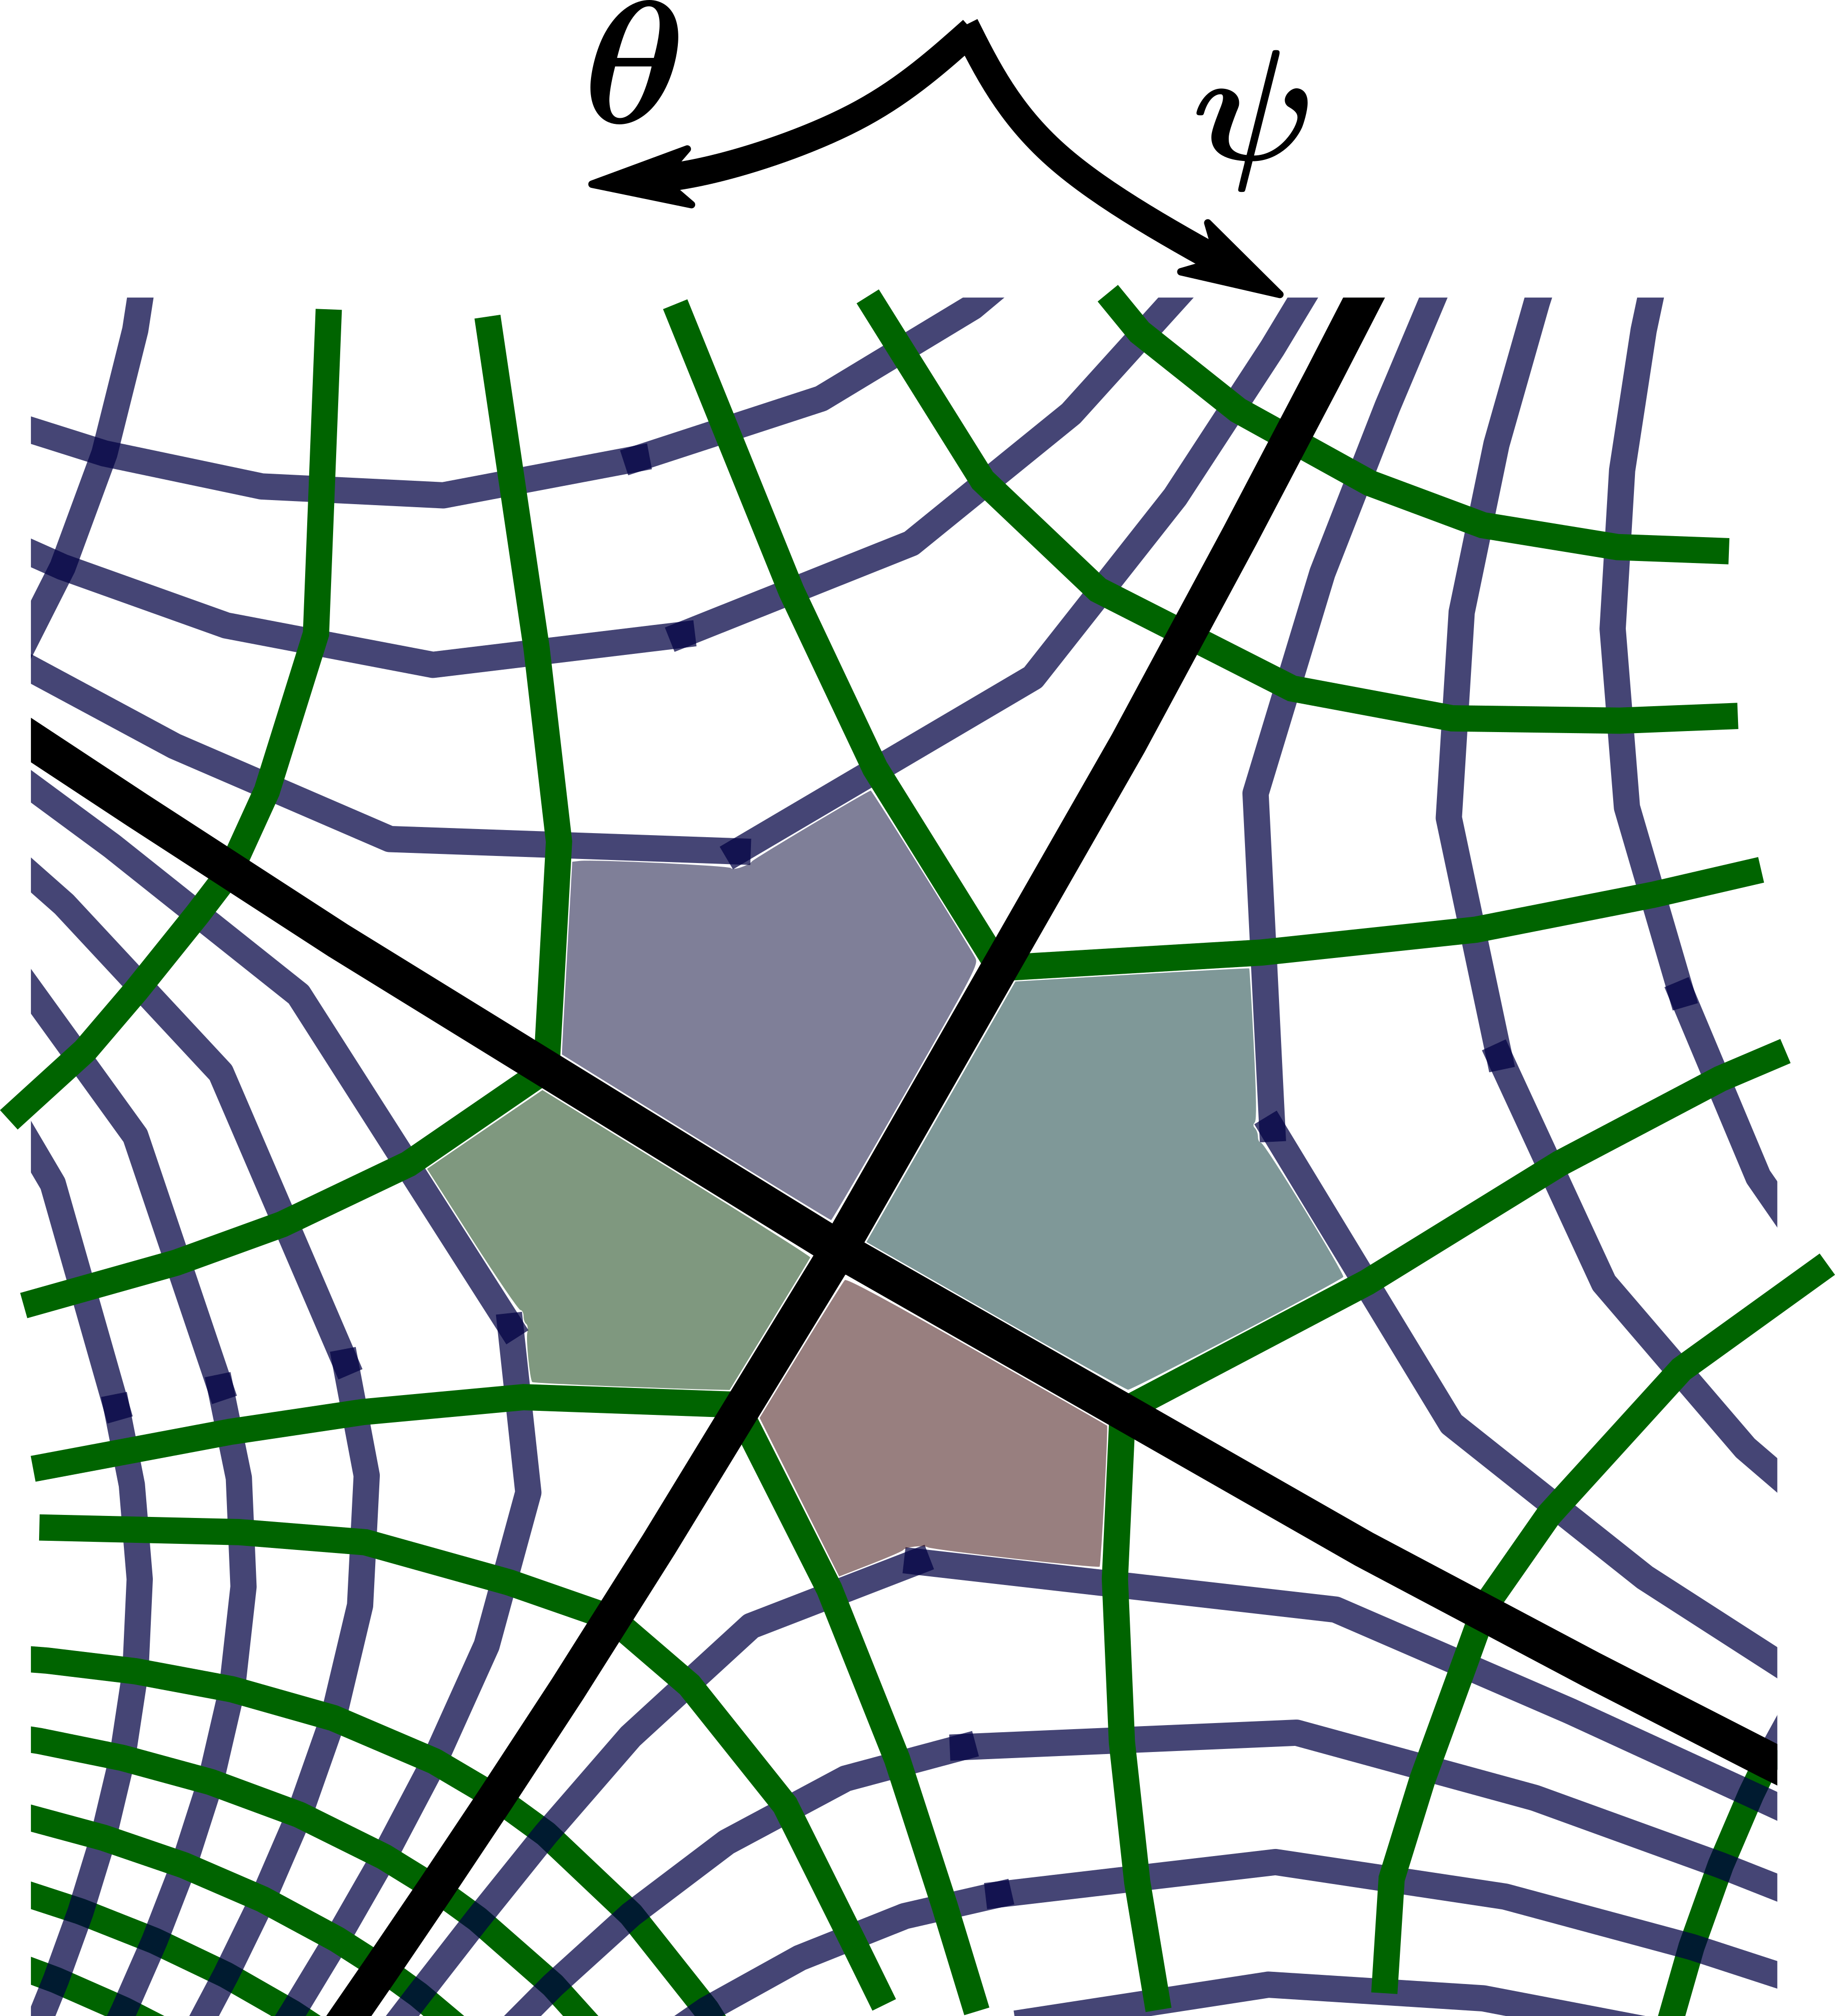
\includegraphics[width=1\textwidth]{schemes/XpointStaggered.png}
		\subcaption{View of staggered cells}
		\label{fig:StaggeredXpoint}
	\end{subfigure}
	\caption{ Sketches of the mesh around the X-point. For collocated cells (a), 8 cells touch the X-point at a corner. For staggered cells (b), the X-point is located at the radial face of 4 cells, effectively modifying the shape of the cells to pentagons. Fluxes across the involved faces are hence ill-defined. }
	\label{fig:XpointDiscretization}
\end{figure}




\section{Implicit-explicit solving procedure}

The model uses an explicit time discretization for the advection terms and an implicit one for the diffusive terms. In turbulence simulations, we limit ourselves to timescales slower than the cyclotronic frequency $\omega_C$. This applies to all advection phenomena, as well as to friction, pressure, and energy source terms, which can then comfortably be solved explicitly in time. \newline

However, ionization/recombination processes, resistive and viscous effects from the Spitzer-Härm model, and electron inertia involve much faster dynamics that would massively constrain the allowed timestep size. Therefore, these terms are solved implicitly. To reduce numerical complexity, they can be decoupled and solved sequentially for the density, the parallel velocity, the temperature, and finally the potentials. 

\subsection{Time discretization schemes}


\subsubsection{Explicit Runge-Kutta solver}


\subsubsection{Implicit-explicit VSIMEX solver}

The time discretization is based on a variable stepsize implicit-explicit scheme (VSIMEX) \cite{wang2008variable}, associating explicit time discretization for the advection terms and an implicit one for the diffusive terms. In turbulence simulations, we limit ourselves to timescales slower than the cyclotronic frequency $\omega_C$. This applies to all advection phenomena, as well as to friction, pressure, and energy source terms, which can then comfortably be solved explicitly in time. \newline


This multi-step method is implemented for orders 1 to 3, and the timestep is updated such that fluxes and velocities in the simulation domain match a targeted CFL value. \newline



\subsection{Initialization at Restart}
\subsubsection{Electron Inertia}
Use the steady-state Ohm's law from the exisiting profile in $\Phi$.

\subsubsection{Parallel Magnetic Vector Potential}
Solve for the steady-state Ampère's law with the now available profile in $\j_\parallel$. Creation of a new solver class for this purpose.


\subsection{}


\subsubsection{Finite volumes with flutter}

The spatial discretization is based on a second-order conservative finite-volume scheme associated with a 3rd-order WENO reconstruction and Donat, Marquina fluxes for a modified Riemann solver for the advection terms to handle both shocks and complicated smooth solution structures \cite{tamain2016tokam3x, Bufferand2021}. \newline
Each of the In this structure, flutter is treated equivalent to drift velocities. 



\subsubsection{Parallel diffusion operator with flutter}
\label{ssec:3DGunter}

In the magnetostatic setting, the parallel diffusion operator on $v_i$ and $T_\alpha$ can be solved independently on each flux surface in a 2D system on the $\theta - \varphi$ plane. The scheme developed by Günter et al. \cite{gunter2005} has proven well-suited to solve the 2D parallel Laplacian equations with minimized numerical spread for highly anisotropic problems. For an operator of the type $\nabla \cdot (\kappa \nabla_\parallel \circ \mathbf{b} )$, parallel gradients are first calculated in cell corners with finite differences and then used in the fluxes across each cell face to get the divergence. The corners where gradients are calculated are shown in Figure \ref{fig:Gunter2D}. This scheme is particularly effective if the poloidal and toroidal components $b^\theta$ and $b^\varphi$ of the contravariant magnetic unit vector in the curvilinear metric have similar magnitudes. This is usually enforced through careful mesh generation. \newline

However, with flutter (Sec. \ref{sec:flutter}), magnetic flux surfaces are no longer aligned to the $\theta - \varphi$ plane because of the new radial component $b^\psi$. As a consequence, all independent 2D problems across flux surfaces are now coupled into a single 3D problem. For the parallel diffusion solver, a first approach would be to extend the above scheme by calculating gradients in the 3D corners of our cells. However, the new component $b^\psi$ is a pure fluctuation, which is therefore expected to be much smaller than $b^\theta$ or $b^\varphi$ and can even vanish locally. This results in significant spurious numerical diffusion in the radial direction of equilibrium gradients. To prevent this diffusion, and still properly capture radial flutter gradients, only crossed derivatives $b^\theta b^\psi$ and $b^\varphi b^\psi$ as well as the principal radial diffusion $b^\psi b^\psi$ use gradients evaluated at 3D corners, while the equilibrium diffusion remains aligned to the $\theta - \varphi$ plane. Examples of the gradients used in this new scheme are shown in Figs. \ref{fig:Gunter3D_theta} and \ref{fig:GunterD_psi}. The new discretization stencil then corresponds exactly to the equilibrium 2D stencil in the limit $b^\psi=0$. \newline

\begin{figure}[!h]\centering
	\begin{subfigure}[t]{0.32\textwidth}
		\centering
		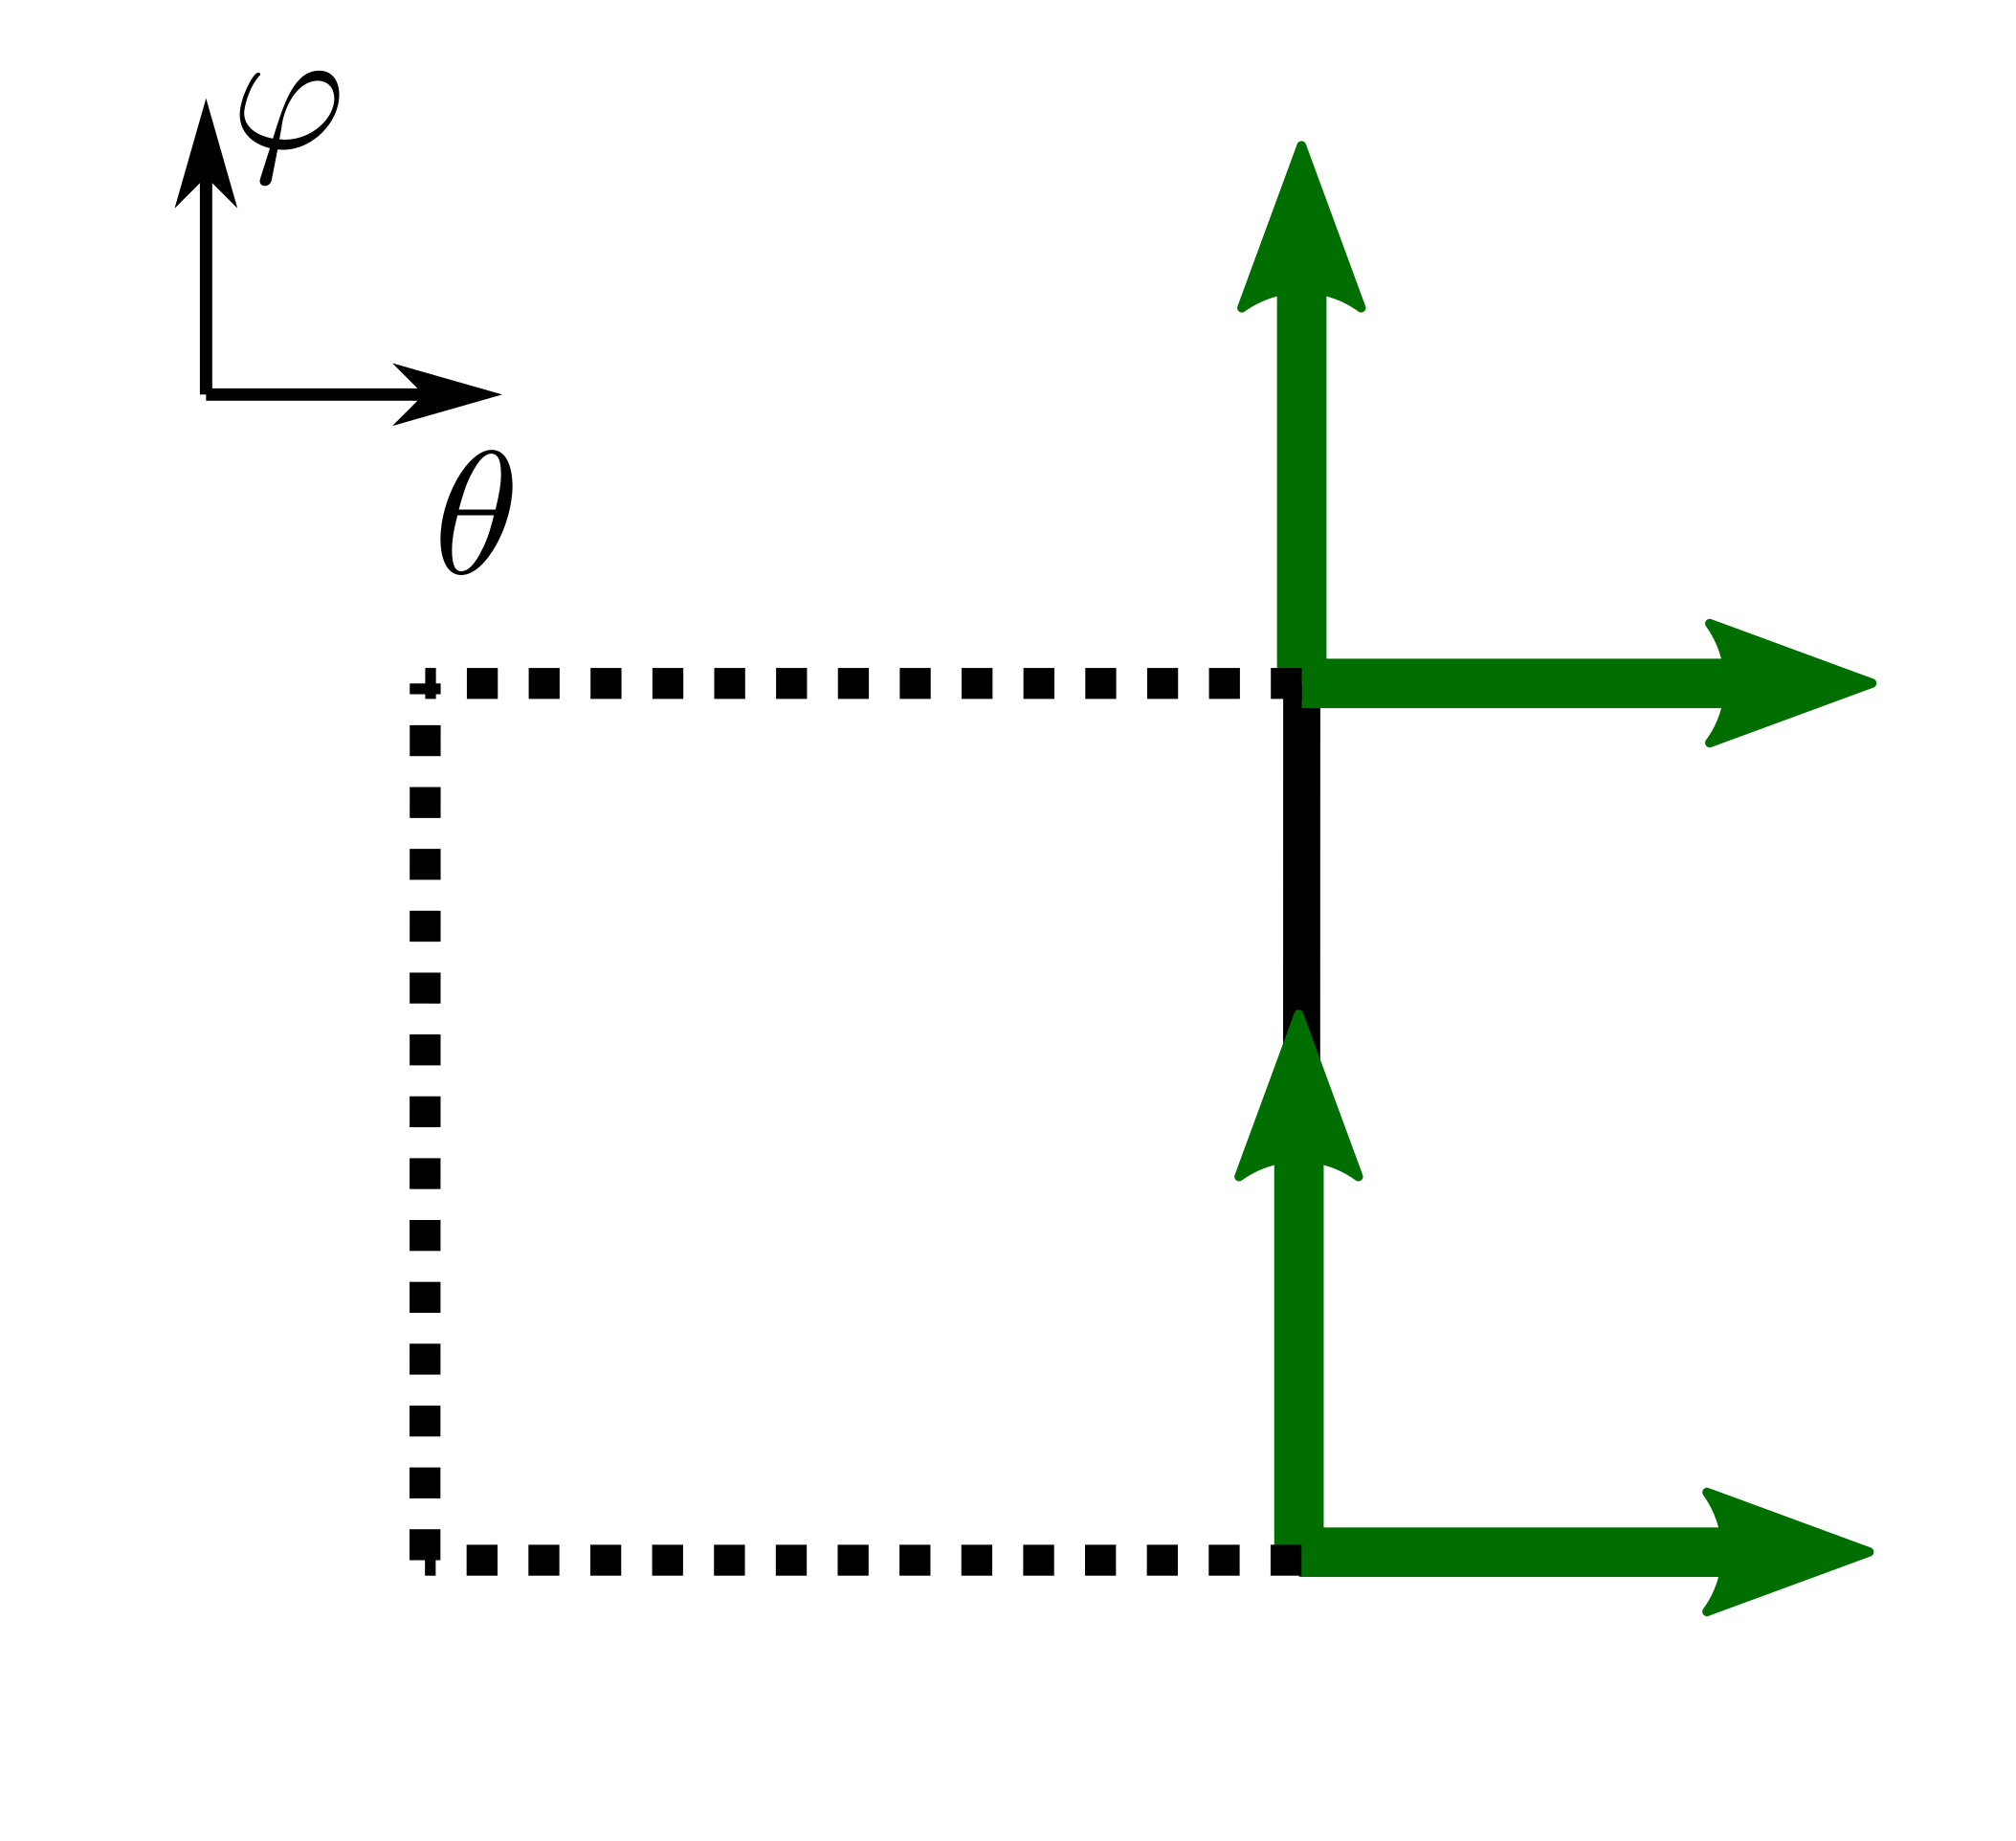
\includegraphics[width=\textwidth]{schemes/Gunter2D.png}
		\caption{ Gradients for the $\theta$-flux without flutter}
		\label{fig:Gunter2D} 
	\end{subfigure}
	\begin{subfigure}[t]{0.32\textwidth}
		\centering
		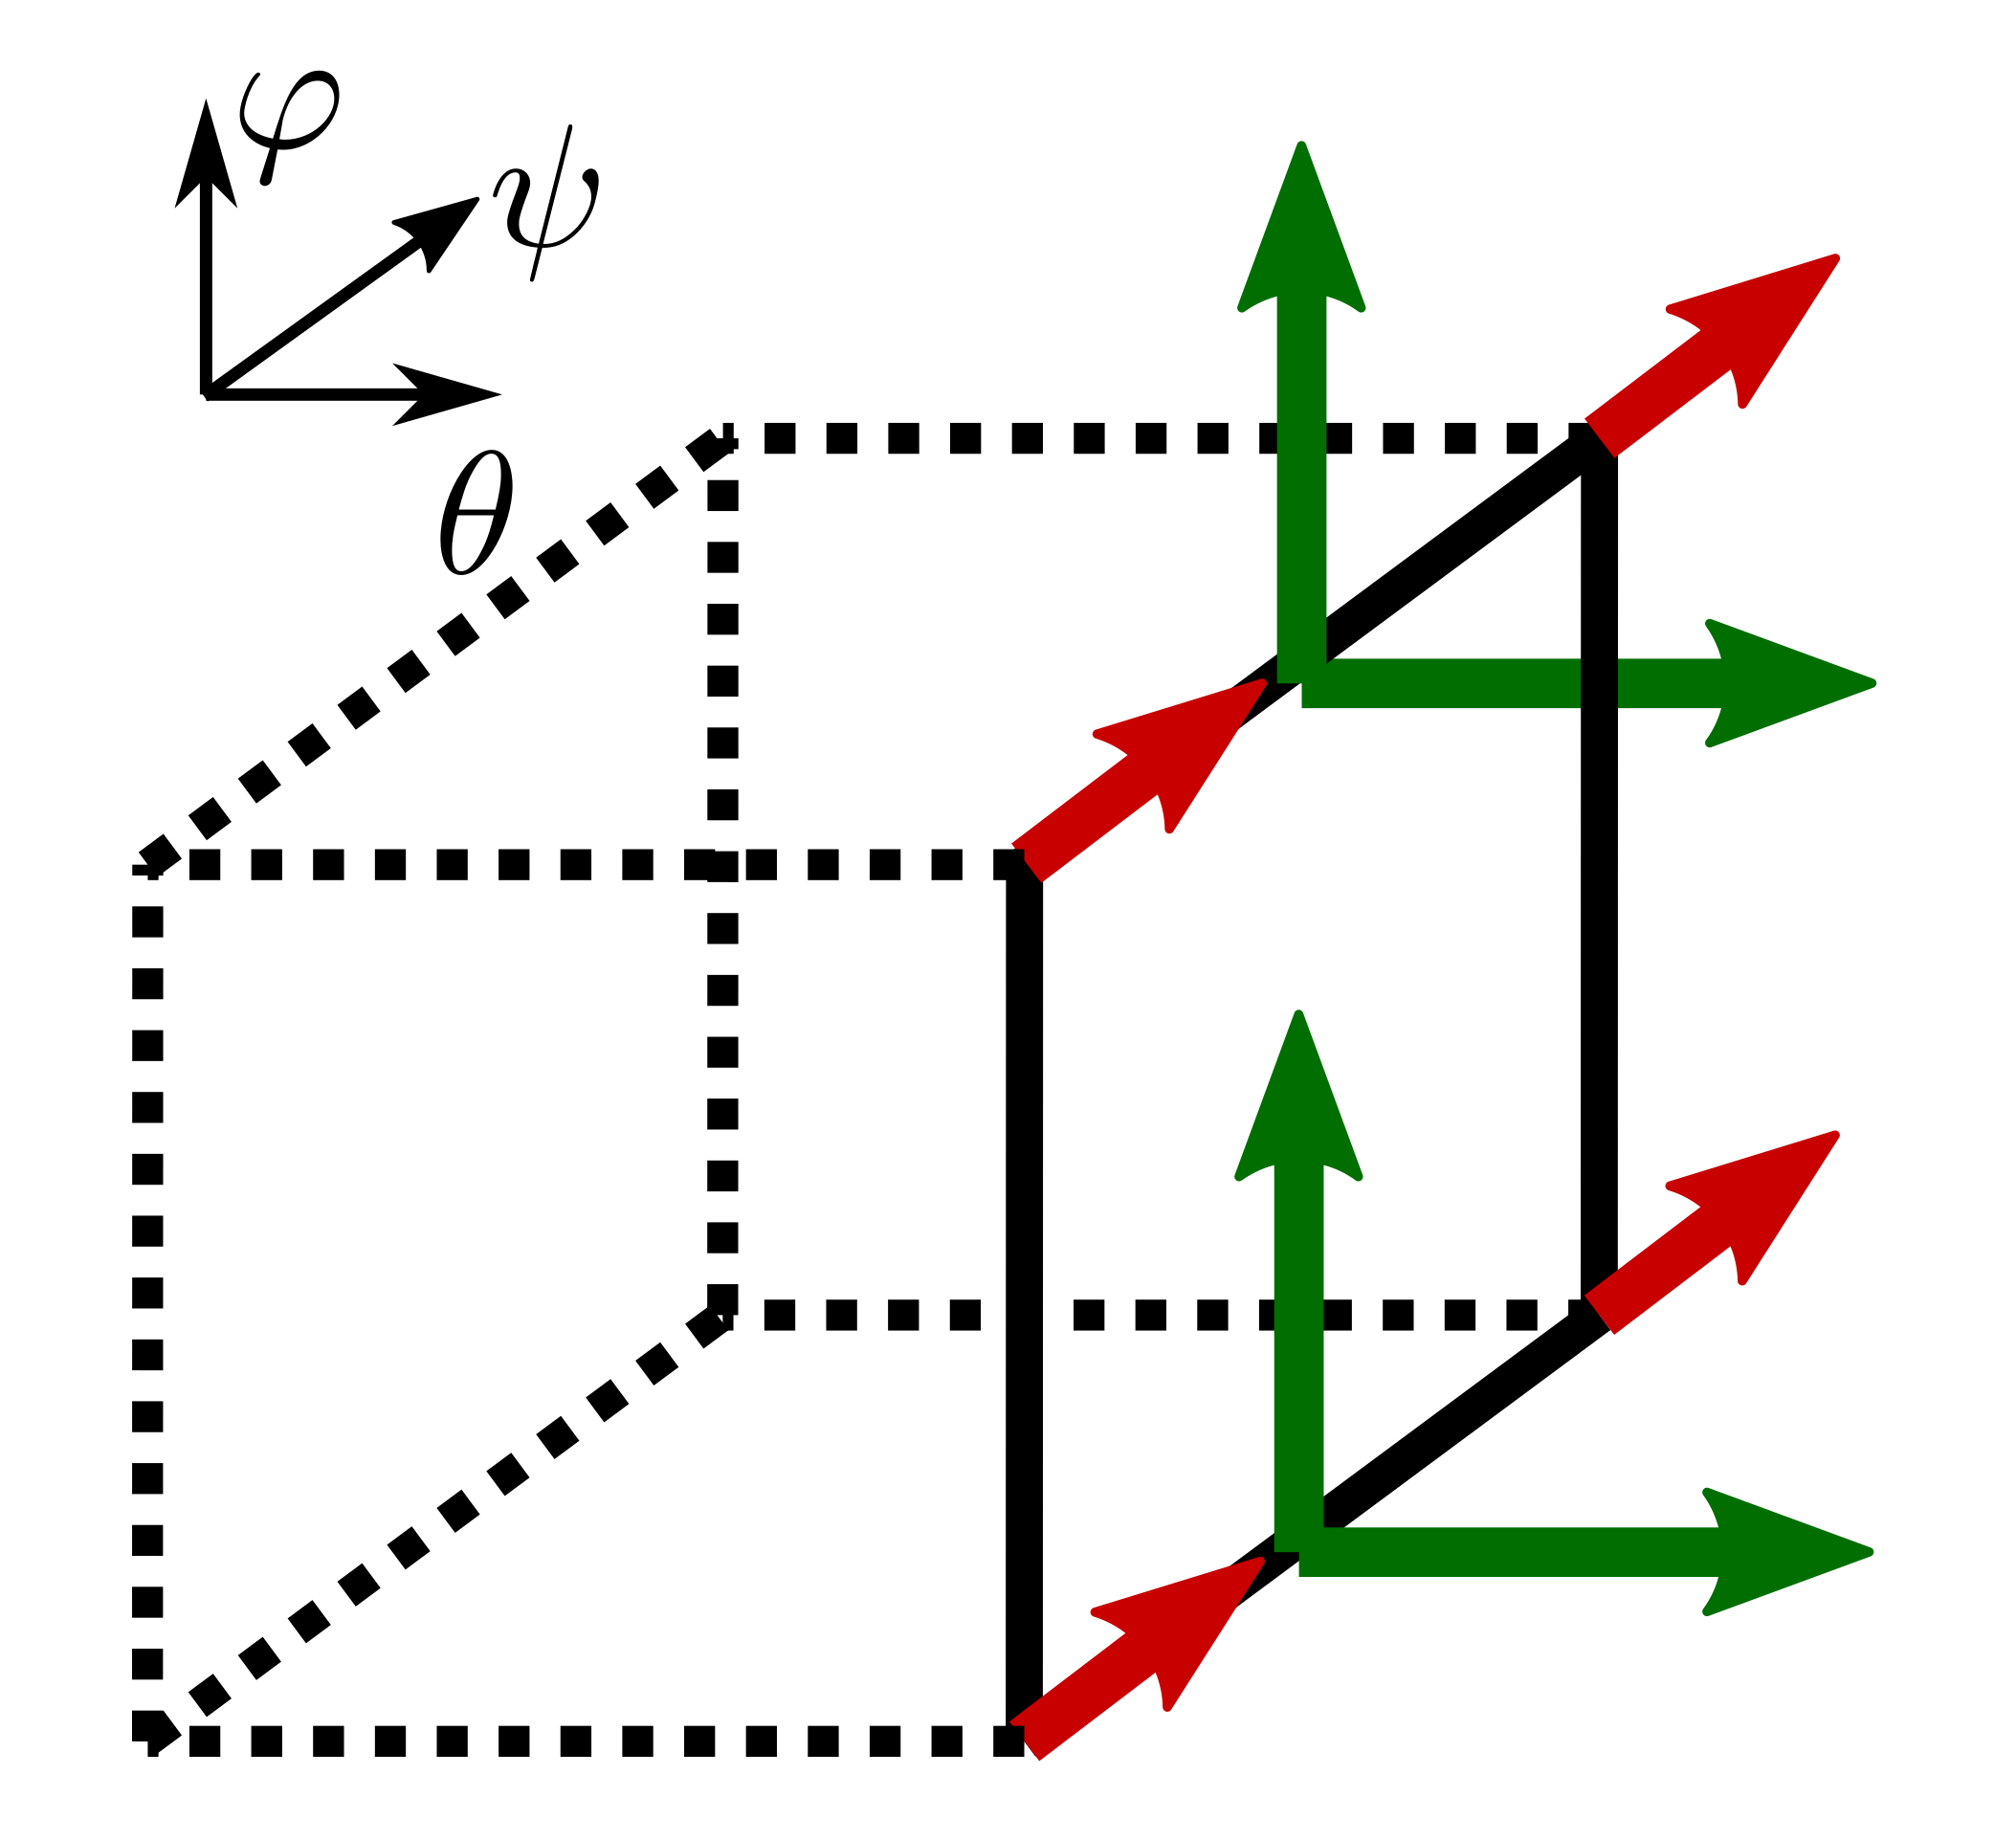
\includegraphics[width=\textwidth]{schemes/Gunter3D_theta.png}
		\caption{ Gradients for the $\theta$-flux with flutter}
		\label{fig:Gunter3D_theta} 
	\end{subfigure}
	\begin{subfigure}[t]{0.32\textwidth}
		\centering
		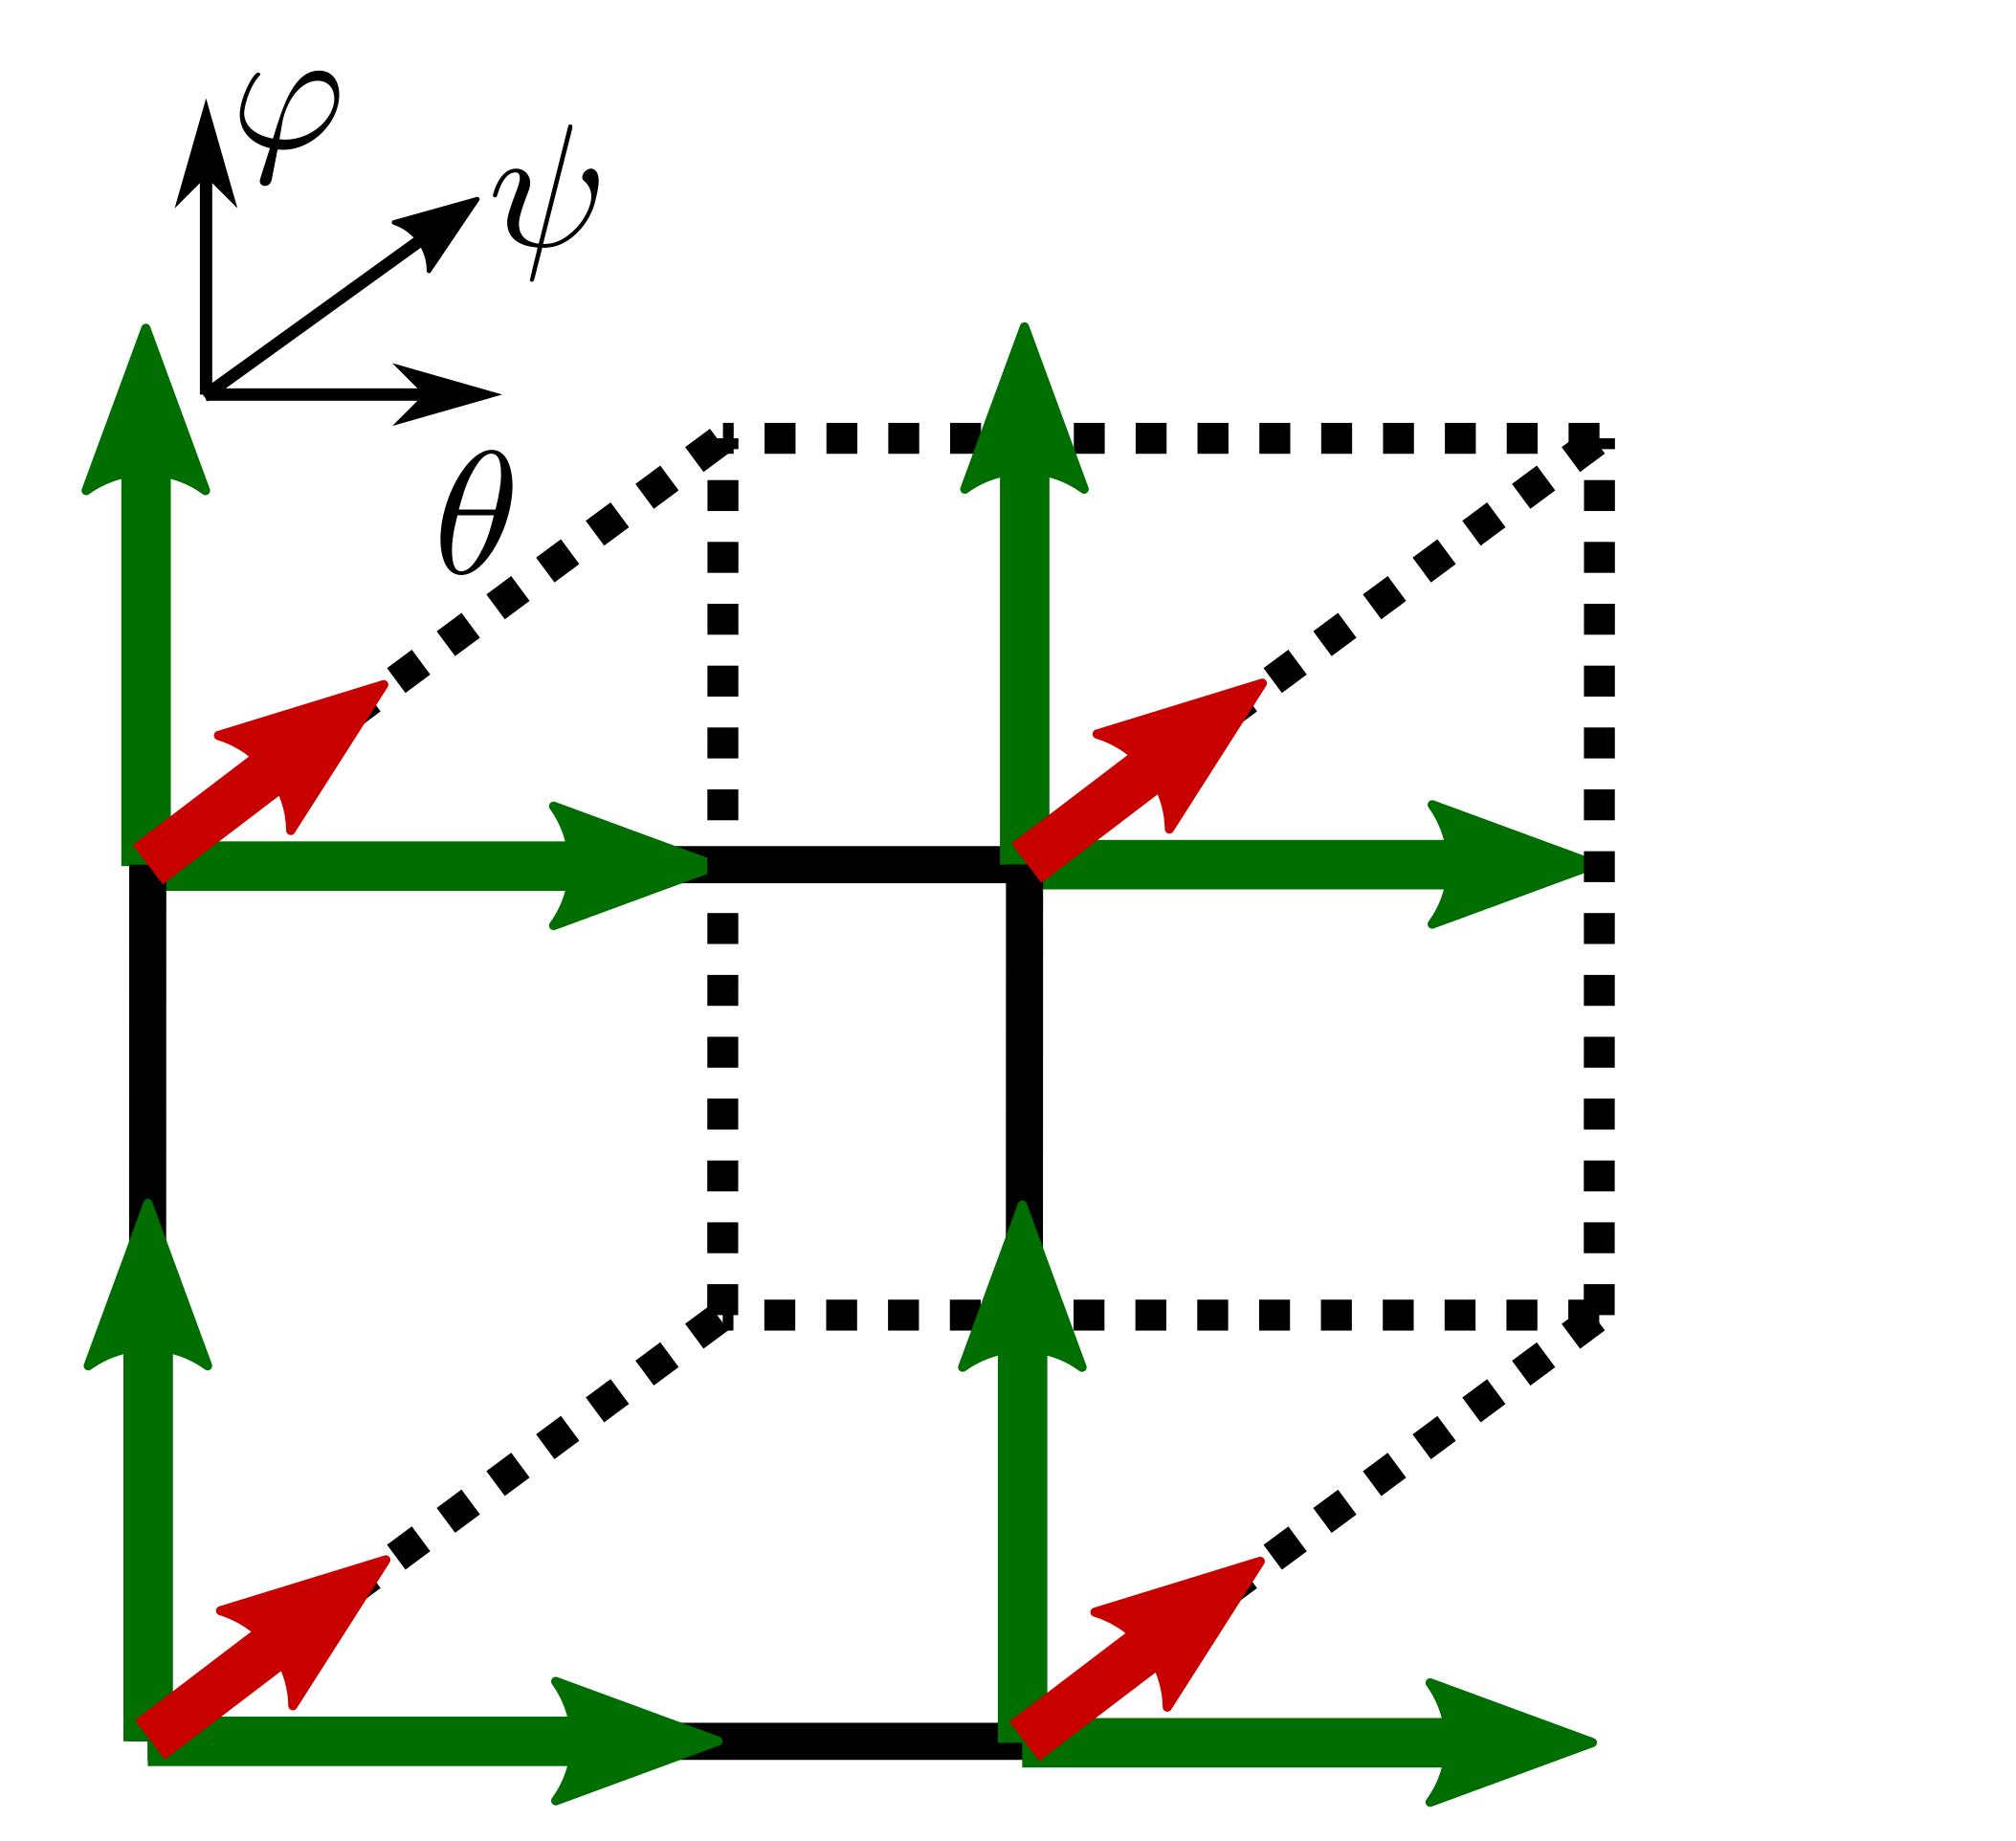
\includegraphics[width=\textwidth]{schemes/Gunter3D_psi.png}
		\caption{ Gradients for the $\psi$-flux with flutter}
		\label{fig:GunterD_psi}
	\end{subfigure}
	\caption{Sketches showing the calculation of gradients for the parallel diffusion scheme. It shows the position where the different gradients are calculated that are relevant for a flux across the cell face with a solid line. Green and red arrows symbolize gradients in the equilibrium and in the radial direction, respectively.}
	\label{fig:GunterStencils_flutter}
\end{figure}






\section{Electromagnetic vorticity system}

The newly introduced fields $j_\parallel$ and $A_\parallel$ are solved implicitly along with the electric potential $\Phi$. As we face a coupled system that connects all points in the domain, direct solvers such as PASTIX are not suitable, especially for fine 3D meshes. We instead prefer to use iterative solvers available in the the PETSc or HYPRE libraries. For the original vorticity system, the Stabilized version of the Biconjugate Gradient method (BiCGStab) along with the Geometric Algebraic Multigrid (GAMG) preconditionner proved to be very efficient and it is desirable to use them on the new systems. This section describes some special numerical features in the construction of the system to facilitate the convergence of the above iterative scheme. \autoref{ssec:equilibrationBLockMatrices} introduces specific row and column scaling to equilibrate the blocks in the new system and \autoref{ssec:StaggeredFieldsMatrix} describes how to handle staggered fields to be compatible with the iterative scheme.

\subsection{Matrix formulation of the electromagnetic system}

With the values for $n_e$ and $T_e$ known at time-step $n+1$, the vorticity equation (Eq. \ref{eq:VorticityEquation}) corresponds to a 3D costly system involving $\Phi$, $j_\parallel$, and $A_\parallel$. To solve it efficiently, the $j_\parallel$ advection and perpendicular diffusion are treated explicitly, allowing the integration of Ohm's law into the vorticity equation and Ampère's law. Then, at time-step $n+1$, the following dimensionless system coupling the two potentials $\Phi$ and $A_\parallel$ must be solved: \newline

\begin{align}
		\label{eq:impl_implicitVorticitySystem}
	\begin{pmatrix}
		\nabla \cdot \left[ D_\perp \nabla_\perp \circ \right] + \nabla \cdot \left[ D_\parallel \nabla_\parallel \circ \mathbf{b} \right]  
		& \frac{\beta_0}{\delta_t} \nabla \cdot \left[ D_\parallel \circ \mathbf{b} \right] \\
		-D_\parallel \nabla_\parallel \circ &
		\frac{\beta_0}{\delta_t} D_\parallel \circ - \nabla \cdot \left[ \nabla_\perp \circ \right]
	\end{pmatrix}
	\begin{pmatrix}
		\Phi^{n+1} \\ A_\parallel^{n+1}
	\end{pmatrix} 
	= \nonumber \\
	\begin{pmatrix}
		\nabla \cdot \left[ D_t j^{n}_\parallel \mathbf{b} \right] + \text{RHS}^\Phi \\
		D_t j^{n}_\parallel + \text{RHS}^{A_\parallel}
	\end{pmatrix}
\end{align}

with $D_\perp = \frac{m_i n_i}{B^2 \delta_t}$, $D_\parallel = \frac{1}{\eta_\parallel + \mu}$, $D_t = \frac{\mu}{\eta_\parallel + \mu}$, and $\mu = m_e / (n_e \delta_t)$ accounting for electron inertia effects. The parameter $\delta_t$ derives from the integration scheme and is equal to the time-step in the case of a first-order implicit Euler scheme. \newline

Since $\eta_\parallel \propto T_e^{-1.5}$, the parallel resistivity $\eta_\parallel$ is often a small parameter that leads to strong anisotropy between the perpendicular and parallel Laplacian operators. However, the electron inertia term, being implemented in the current solver, acts as an upper limit for the parallel diffusion coefficient, which is expected to improve the matrix conditioning as $\eta_\parallel$ approaches zero. This is in contrast to the original electrostatic model from \cite{Bufferand2021}. \newline


\subsubsection{Equilibration of the Matrix Blocks}
\label{ssec:equilibrationBLockMatrices}
The matrices in the electromagnetic model \autoref{sec:DedimensionalizedElectromagneticModelS3X} can be decomposed in 2x2 or 3x3 block matrices that apply on the respective fields $\Phi$, $A_\parallel$ and/or $j_\parallel$. Apart of the use of dedimensionalized quantities, no effort was made so far to ensure that the blocks are roughly of the same order of the magnitude, which is important for the condition number of the matrix, nor that the matrix is diagonally dominant, which is generally a desirable feature for fast convergence of iterative schemes. \\
In the following bits, we introduce some column $c_X$ and row $r_X$ scaling factors that are specific to the blocks $X$ of the matrix such that the above conditions are fullfilled as well as possible. To ensure a correct solution, the row scaling factor $r_X$ must be applied to the corresponding entry in the RHS vector and as a matter of fact, in the original vorticity matrix, we already have $r_\Phi = J$ the metrical Jacobian from \autoref{ssec:MetricCurvilinearCoordinates} to remove the effect of different mesh sizes in the domain on the discrete Laplacian operators. The column scaling factors $c_X$ must be taken care of when retrieving the fields from the numerical solution and it is strongly recommended to apply them to the initial guess for the iterative scheme. \\ 
Some exisiting algorithms optimize the scaling task such as  --- cite ----. However, they all require an expensive matrix analysis phase that must be repeated regularly since the matrix changes with the progress of the simulation. Therefore, we use the knowledge about the construction of the matrix blocks to define sufficiently good scaling factors. An educated row and column scaling can considerably increase the condition number of a matrix\cite{van1969condition}.\\

Due to the large size of the system, it must be resolved using iterative solvers. Note that the two diagonal blocks already have a convenient shape, and the anti-diagonal blocks contain parallel divergence and gradient operators, whose discrete stencils are very similar. Therefore, by scaling both the second column and row with $\sqrt{\delta_t / \beta_0}$, the resulting matrix becomes almost symmetric, which is convenient for most iterative solvers.


\subsubsection{Staggered Fields in the Matrix}
\label{ssec:StaggeredFieldsMatrix}
The GAMG multigrid solves the system on different coarser levels by restricting the matrix and the RHS vector and then interpolates the solution back to the finer levels. In the new system, two consecutive entries belong to different fields, which makes the whole restriction-interpolation task obsolete from the very first level since neither the solution nor the matrix entries are similar between neighbours. In general, PETSc takes care of multiple fields in a coupled system if one defines a block size (in our case either 2 or 3) that indicates GAMG how to match corresponding entries.vim  However, as seen in \autoref{ssec:SpatialDiscretization}, the fields $A_\parallel$ and $j_\parallel$ are defined on a staggered grid in poloidal and toroidal directions as opposed to the collocated field for $\Phi$. For the system it means that at each wall in negative directions (at the left target and for non-axisymmetric geometries), a line and column for $\Phi$ exists but not for the two other fields. This in turn is problematic for GAMG as the blocks are globally defined and two different fields would again end up together and the total system size might even not be a multiple of the blocksize (2 resp. 3), which at all prevents the initialization of the preconditioner. \\


\subsection{Treatment of flutter}

\subsubsection{Parallel diffusion on $\Phi$}
For the parallel diffusion on the electric potential $\nabla \cdot \left[ D_\parallel \nabla_\parallel \Phi \mathbf{b} \right]$ with flutter, we do not use the stencil introduced in Sec. \ref{ssec:3DGunter}. To avoid numerical difficulties and the appearance of unphysical modes, the discretization of this term needs to be consistent with the parallel gradient and divergence operators in the same system. Since the grid for $A_\parallel$ and $j_\parallel$ is only staggered in the $\theta$ and $\varphi$ directions, we do not know them in the radial corners from Figs. \ref{fig:Gunter3D_theta} and \ref{fig:GunterD_psi}. Instead, the discrete diffusion operator is defined as the combination of the operators for the gradient and the divergence. It involves two neighbors on both radial sides, so the resulting stencil is less compact but consistent with the remaining system. Note that in cases without flutter ($b^\psi = 0$), the diffusion operator exactly corresponds to Günter's scheme \cite{gunter2005} because the staggered fields are known at the position of the green gradients in Fig. \ref{fig:GunterStencils_flutter}. \newline




\subsection{Evaluation of the condition number}

The electromagnetic vorticity system needs to be solved implicitly, and the condition number of the matrix is an important property that essentially defines the speed of convergence of iterative solvers. Extensive research in the past decade\cite{pyzara2011influence, strakos1991linear, drkovsova1995numerical, greenbaum1997numerical}, particularly on GMRES and conjugate gradient methods as they are used in SOLEDGE3X, has shown that a high condition number results in an increased number of iterations to reach convergence. The condition number of a matrix $\textbf{M}$ is defined as the ratio between its largest and smallest eigenvalues:

\begin{equation}
	\label{eq:Impl_defConditionNumber}
	\kappa\left(\textbf{M}\right) = \frac{\left|\lambda_{\text{max}}(\textbf{M})\right|}{\left|\lambda_{\text{min}}(\textbf{M})\right|}
\end{equation}

It is therefore of particular interest to investigate how the electromagnetic extension of the system affects the conditioning of the vorticity system. While there are efficient algorithms to estimate the largest eigenvalue of a matrix, the smallest is much more expensive to compute. For the large 3D vorticity system, directly calculating the condition number is not feasible. Instead, we approach this question analytically. \\

Consider a 2D orthonormal system, with perpendicular gradients exclusively in the $x$ direction and parallel gradients in the $y$ direction, with $N_x \times N_y$ discretization points. All fields are assumed to take some constant reference value, the timestep size is fixed to $\delta_t$, and time advancement is performed using the first-order implicit Euler method. Without a curvilinear grid, the gradient and divergence stencils are identical, and with the row/column scaling from Sec. \ref{ssec:equilibrationBLockMatrices}, the vorticity system can then be expressed as:


\begin{equation}
	\textbf{M} = 
	\begin{pmatrix}
		\alpha \textbf{L}_\perp + \sigma \textbf{L}_\parallel & \gamma \textbf{G}_\parallel \\ -\gamma \textbf{G}_\parallel^T & \sigma \textbf{I} - \gamma^2\textbf{L}_\perp
	\end{pmatrix}
\end{equation}

where $\alpha = \frac{m_in_i}{B^2\delta_t}$, $\sigma = \frac{1}{\eta_\parallel + \frac{m_e}{n_e \delta_t}}$, and $\gamma = \sqrt{\frac{\delta_t }{\beta_0}}$. The stencil matrices $\textbf{L}_\perp$ and $\textbf{L}_\parallel$ describe the Laplacians between the $x$ and $y$ neighbors, respectively, while $\textbf{G}_\parallel$ represents the gradient over $y$. Their matrices take the following forms:

\begin{align}
	\mathbf{L}_\perp =& \begin{pmatrix}
		-2 & 1 & 0 & \cdots & 0 \\
		1 & -2 & 1 & \cdots & 0 \\
		0 & 1 & -2 & \cdots & 0 \\
		\vdots & \vdots & \vdots & \ddots & \vdots \\
		0 & 0 & 0 & \cdots & -2
	\end{pmatrix}_{N_x \times N_x} &
	\mathbf{L}_\parallel =& \begin{pmatrix}
		-2 & 1 & 0 & \cdots & 1 \\
		1 & -2 & 1 & \cdots & 0 \\
		0 & 1 & -2 & \cdots & 0 \\
		\vdots & \vdots & \vdots & \ddots & \vdots \\
		1 & 0 & 0 & \cdots & -2
	\end{pmatrix}_{N_y \times N_y} \nonumber\\
	\mathbf{G}_\parallel =& \begin{pmatrix}
		-1 & 1 & 0 & \cdots & 0 \\
		0 & -1 & 1 & \cdots & 0 \\
		\vdots & \vdots & \vdots & \ddots & \vdots \\
		1 & 0 & 0 & \cdots & -1
	\end{pmatrix}_{N_y \times N_y}
\end{align}

In order to make the system invertible and avoid an infinite condition number, we assume Dirichlet-0 boundary conditions in the perpendicular direction and periodic boundary conditions in the parallel direction. This can be viewed as a region of closed flux surfaces connected to a region with a very crude sheath-dominated plasma. We can compute the eigenvalues of the two Laplacians and the gradient coupling matrix exactly.

\begin{align}
	\lambda_{k_x}(\mathbf{L}_\perp) =& 4\sin^2\left(\frac{(k_x+1)\pi}{2N_x}\right)  & \lambda_{k_y}(\mathbf{L}_\parallel) =& 4\sin^2\left(\frac{k_y\pi}{N_y}\right) & \lambda_{k_y}(\mathbf{G}_\parallel) = i\sin\left(\frac{k_y\pi}{N_y}\right)
\end{align}

where $k_x\in[0,N_x-1]$ and $k_y\in[0,N_y-1]$ are indices for all eigenvalues. We observe that both parallel systems have a zero eigenvalue that corresponds to a constant mode, due to the periodic boundary conditions along the closed flux surfaces, indicating that the solution can be determined up to a constant. The perpendicular operators, with fixed boundaries, make the system invertible with a unique solution. 

Let us now evaluate the extremal eigenvalues of the diagonal blocks of $\mathbf{M}$. For the upper-left block, which contains the sum of Laplacians, the eigenvalues correspond to the combinations of $(k_x,k_y)$ such that $|\lambda_{k_x}|+|\lambda_{k_y}|$ is minimized or maximized:

\begin{align}
	\label{eq:Impl_EVupperLeftBlock}
	\lambda_{min}(\alpha \textbf{L}_\perp + \sigma \textbf{L}_\parallel) &= \alpha\cdot\frac{\pi^2}{N_x^2} & \lambda_{max}(\alpha \textbf{L}_\perp + \sigma \textbf{L}_\parallel) &= 4(\alpha + \sigma)
\end{align}

For the lower-right block matrix, the identity matrix will shift the eigenvalues of the perpendicular Laplacian by $\sigma$:

\begin{align}
	\label{eq:Impl_EVlowerRightBlock}
	\lambda_{min}(\sigma \textbf{I} - \gamma^2 \textbf{L}_\perp) &= \sigma - 4\gamma^2 & \lambda_{max}(\sigma \textbf{I} - \gamma^2 \textbf{L}_\perp) &= \sigma - \gamma^2\frac{\pi^2}{N_x^2}
\end{align}

For sufficiently large systems, the largest eigenvalue will be on the order of $\sigma$. If $\sigma \gg \gamma^2$, all eigenvalues will be close to $\sigma$, resulting in an excellent matrix condition. However, if $\sigma < 4\gamma^2$, some eigenvalues may become negative, causing the system to lose its positive-definiteness. This can lead to strong instabilities, and standard iterative solvers (e.g., GMRES or BiCGStab) may fail or produce unreliable results, as these methods are generally designed for positive-definite matrices. To ensure that the problem remains well-posed, we must enforce the constraint:

\begin{equation}
	\label{eq:Impl_conditionPositiveDefinite}
	\frac{1}{4}\beta_0 > \delta_t\eta_\parallel + \frac{m_e}{n_e} 
\end{equation}

This condition states that $\beta_0$ cannot be too small for the system to remain solvable. Assuming this lower condition on $\beta_0$ holds with a sufficient margin, the minimum and maximum eigenvalues in Eq. \ref{eq:Impl_EVlowerRightBlock} are simply $\lambda_{min} = \lambda_{max} = \sigma$. \\

We now have all extremal eigenvalues along the block diagonal. For the combined matrix $\mathbf{M}$, the gradient coupling plays a crucial role. If the coupling is small, the eigenvalues of $\mathbf{M}$ are given by the union of the eigenvalues of the diagonal blocks. The condition number of $\mathbf{M}$ is then the ratio of the overall maximum and minimum eigenvalues of the block matrices. Since $\gamma$ is certainly smaller than $\sigma$, we should investigate the impact of the coupling in more detail. The matrix $\mathbf{M}$ can be transformed into a block diagonal form by applying the Schur complement $\mathbf{S}$ on the lower-left block.


\begin{align}
	\textbf{M} = \begin{pmatrix}
		\textbf{A} & \textbf{B} \\ -\textbf{B}^T & \textbf{C} 
	\end{pmatrix} &= \begin{pmatrix}
		\textbf{I} & 0 \\ -\textbf{B}^T\textbf{A}^{-1} & \textbf{I}
	\end{pmatrix}\begin{pmatrix}
		\textbf{A} & 0 \\ 0 & \textbf{S}
	\end{pmatrix}\begin{pmatrix}
		\textbf{I} & \textbf{A}^{-1}\textbf{B} \\ 0 & \textbf{I}
	\end{pmatrix} & \text{with: } 
	\textbf{S} = \textbf{D} + \textbf{B}^T \textbf{A}^{-1}\textbf{B}
\end{align}


The block diagonal matrix is multiplied by both a lower and an upper diagonal matrix. Since they are invertible and all diagonal elements are equal to 1, the block diagonal matrix is quasi-similar to $\textbf{M}$\cite{gallier2010schur}, thereby preserving its eigenvalues. Calculating the eigenvalues of the block diagonal matrix gives us then a good approximation for the actual eigenvalues of $\textbf{M}$. We now need to estimate the eigenvalues of the Schur complement. Given that $\textbf{A}$ is Laplacian-based, the eigenvalues of $\textbf{A}^{-1}$ are the reciprocals of the eigenvalues of $\textbf{A}$, as shown in Eq. \ref{eq:Impl_EVupperLeftBlock}. The matrix is sandwiched between the gradient operator and its transpose, and together they behave like a parallel Laplacian with the scaling factor $\gamma^2$. We can first estimate:

\begin{align}
	\lambda_{min}(\textbf{B}^T \textbf{A}^{-1}\textbf{B}) &= \frac{\gamma^2\lambda_{min}(L_\parallel)}{\lambda_{max}(\alpha \textbf{L}_\perp + \sigma \textbf{L}_\parallel)} = 0 \\ 
	\lambda_{max}(\textbf{B}^T \textbf{A}^{-1}\textbf{B}) &= \frac{\gamma^2\lambda_{max}(L_\parallel)}{\lambda_{min}(\alpha \textbf{L}_\perp + \sigma \textbf{L}_\parallel)} = \frac{4\gamma^2N_x^2}{\alpha\pi^2}
\end{align}

By combining this result with the eigenvalues of $\sigma \textbf{I} - \gamma^2 \textbf{L}_\perp$ from Eq. \ref{eq:Impl_EVlowerRightBlock}, we can estimate the extremal eigenvalues of the Schur complement:

\begin{align}
	\label{eq:Impl_EVschurComplement}
	\lambda_{min}(\textbf{S}) &= \sigma  & 
	\lambda_{max}(\textbf{S}) &= \sigma + \frac{4\gamma^2N_x^2}{\alpha\pi^2}
\end{align}

Everything is now in place to address the eigenvalues of $\mathbf{M}$ with the two block diagonals $\textbf{A}$ and $\textbf{S}$. Recall the assumption $\sigma \gg \gamma^2$ from Eq. \ref{eq:Impl_conditionPositiveDefinite}, thus the double-Laplacian system in Eq. \ref{eq:Impl_EVupperLeftBlock} defines the minimum eigenvalue of $\textbf{M}$. Considering that $\alpha \sim 1/\delta_t$ in the dimensionless equations and $\gamma^2 \sim \delta_t / \beta_0$ is large, we can reasonably expect $\gamma^2 \gg \alpha$. The maximum eigenvalue of $\textbf{M}$ arises from the Schur complement in Eq. \ref{eq:Impl_EVschurComplement}. Therefore, the condition number of $\textbf{M}$ can be estimated as:

\begin{equation}
	\label{eq:Impl_conditionNumberM}
	\kappa(\textbf{M}) \approx \frac{\sigma N_x^2}{\alpha\pi^2} + \frac{4\gamma^2N_x^4}{\alpha^2\pi^4}
\end{equation}

or in terms of dimensionless reference values:

\begin{equation}
	\label{eq:Impl_conditionNumberElectromagneticVorticitySystem}
	\boxed{
		\kappa(\textbf{M}) \approx \frac{ B^2\delta_t N_\perp^2}{m_in_i\pi^2} \cdot \frac{1}{\eta_\parallel + \frac{m_e}{n_e \delta_t}} + \frac{4\delta_t^3 B^4 N_\perp^4}{\beta_0m_i^2n_i^2\pi^4}
	}
\end{equation}

In the case of the system with electron inertia, but without electromagnetic induction, the analysis becomes much simpler as only the double Laplacian block matrix constitutes the system. Its condition number is given by the eigenvalues in Eq. \ref{eq:Impl_EVupperLeftBlock}:

\begin{equation}
	\label{eq:Impl_conditionNumberM_electronInertia}
	\kappa(\textbf{A}) = \frac{4\sigma N_x^2}{\alpha\pi^2} + \frac{4 N_x^2}{\pi^2}
\end{equation}

and is primarily determined by the first term. It can be written as:

\begin{equation}
	\label{eq:Impl_conditionNumberElectrnInertiaVorticitySystem}
	\boxed{
		\kappa(\textbf{A}) \approx \frac{ B^2\delta_t N_\perp^2}{m_in_i\pi^2} \cdot \frac{1}{\eta_\parallel + \frac{m_e}{n_e \delta_t}}
	}
\end{equation}

From these expressions for the condition number, we observe a degradation as the electric resistivity approaches zero, aligning with the difficulties faced by the original electrostatic implementation in higher-power scenarios. The finite electron mass acts as a lower bound for $\eta_\parallel$, which is expected to significantly aid iterative solvers in such scenarios. Magnetic induction introduces the second term in Eq. \ref{eq:Impl_conditionNumberElectromagneticVorticitySystem}, and will always deteriorate the matrix conditioning. However, it is inversely proportional to $\beta_0$, such that the deterioration is limited as the pressure ratio increases. Numerically, electromagnetic effects should only be considered in simulation scenarios where $\beta_0$ is sufficiently large. This point is further emphasized by the condition in Eq. \ref{eq:Impl_conditionPositiveDefinite}, which imposes a lower limit on $\beta_0$ to ensure a positive-definite matrix—an essential property for most iterative solvers. In Fig. \ref{fig:Impl_conditionNumber}, we illustrate how the condition number changes with $\eta_\parallel$, $\delta_t$, and $N_\perp$ for both electrostatic and electromagnetic systems, with and without electron inertia. 

\begin{figure}[H]
	\centering
	\begin{subfigure}[t]{0.30\textwidth}
		\centering
		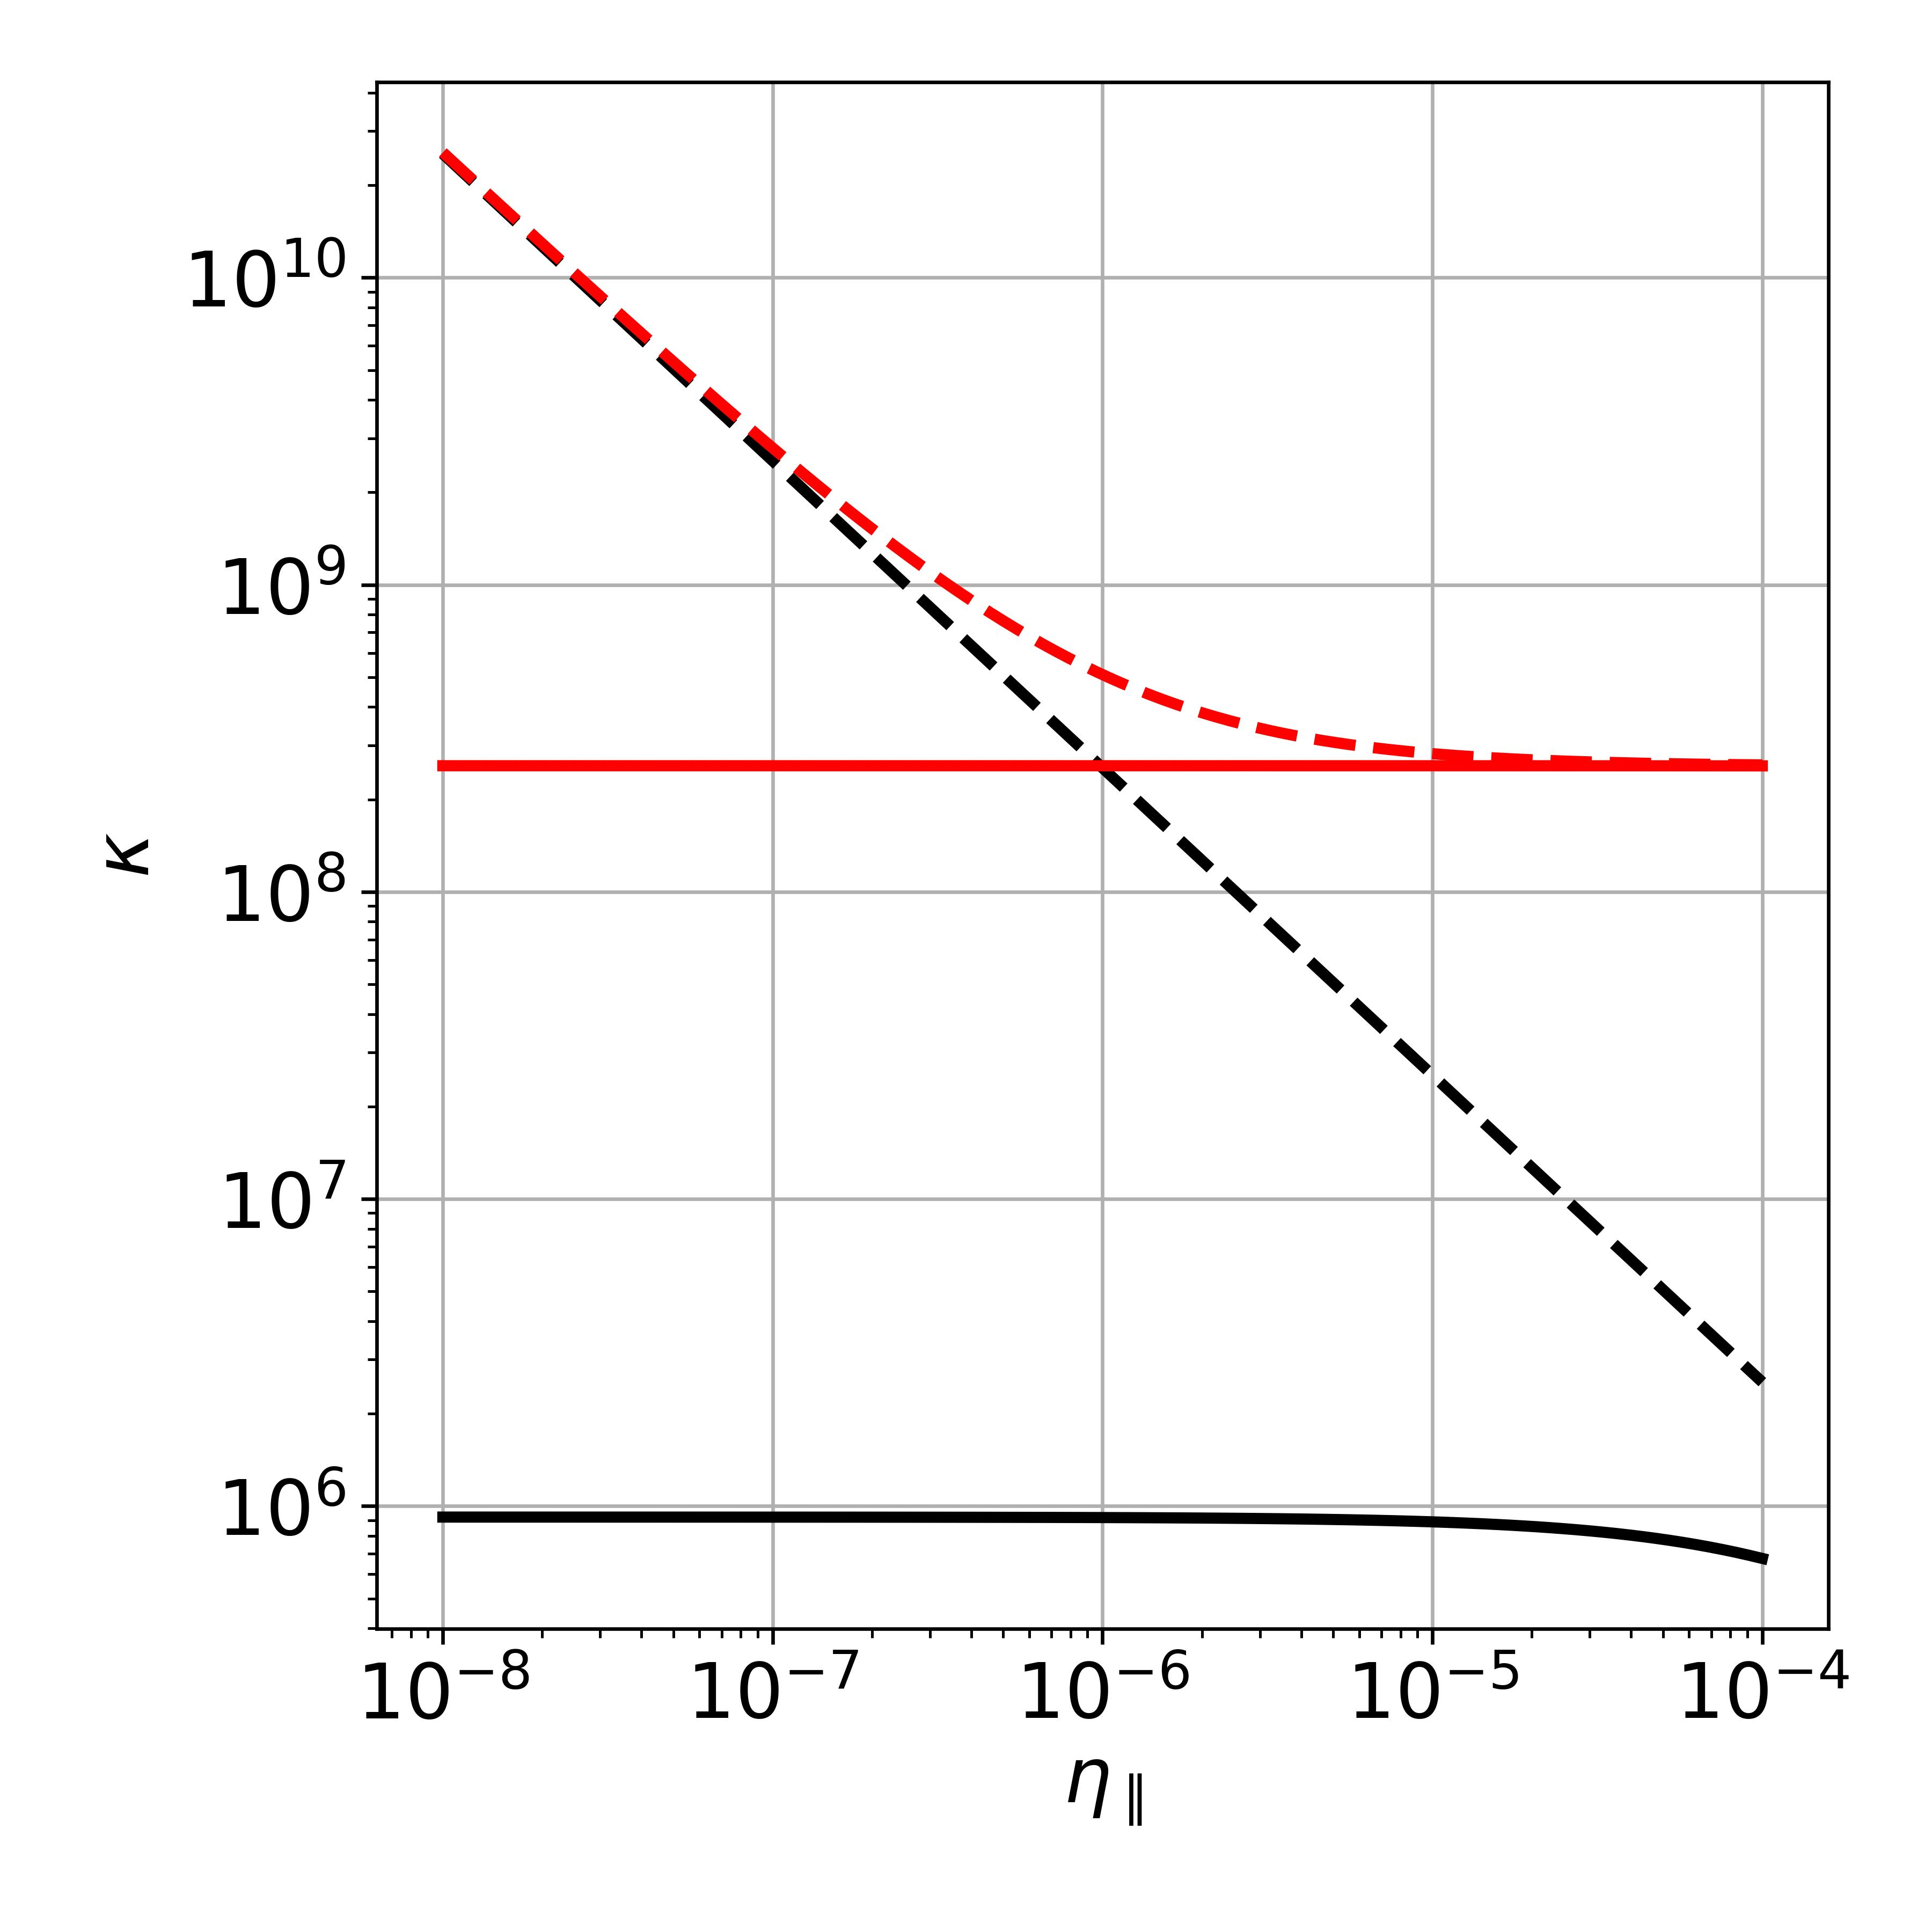
\includegraphics[width=1\textwidth]{schemes/conditionNumber_eta.jpg}
		\subcaption{Parallel electric \\ resistivity $\eta_\parallel$}
		\label{fig:Impl_conditionNumber_eta}
	\end{subfigure}
	\begin{subfigure}[t]{0.30\textwidth}
		\centering
		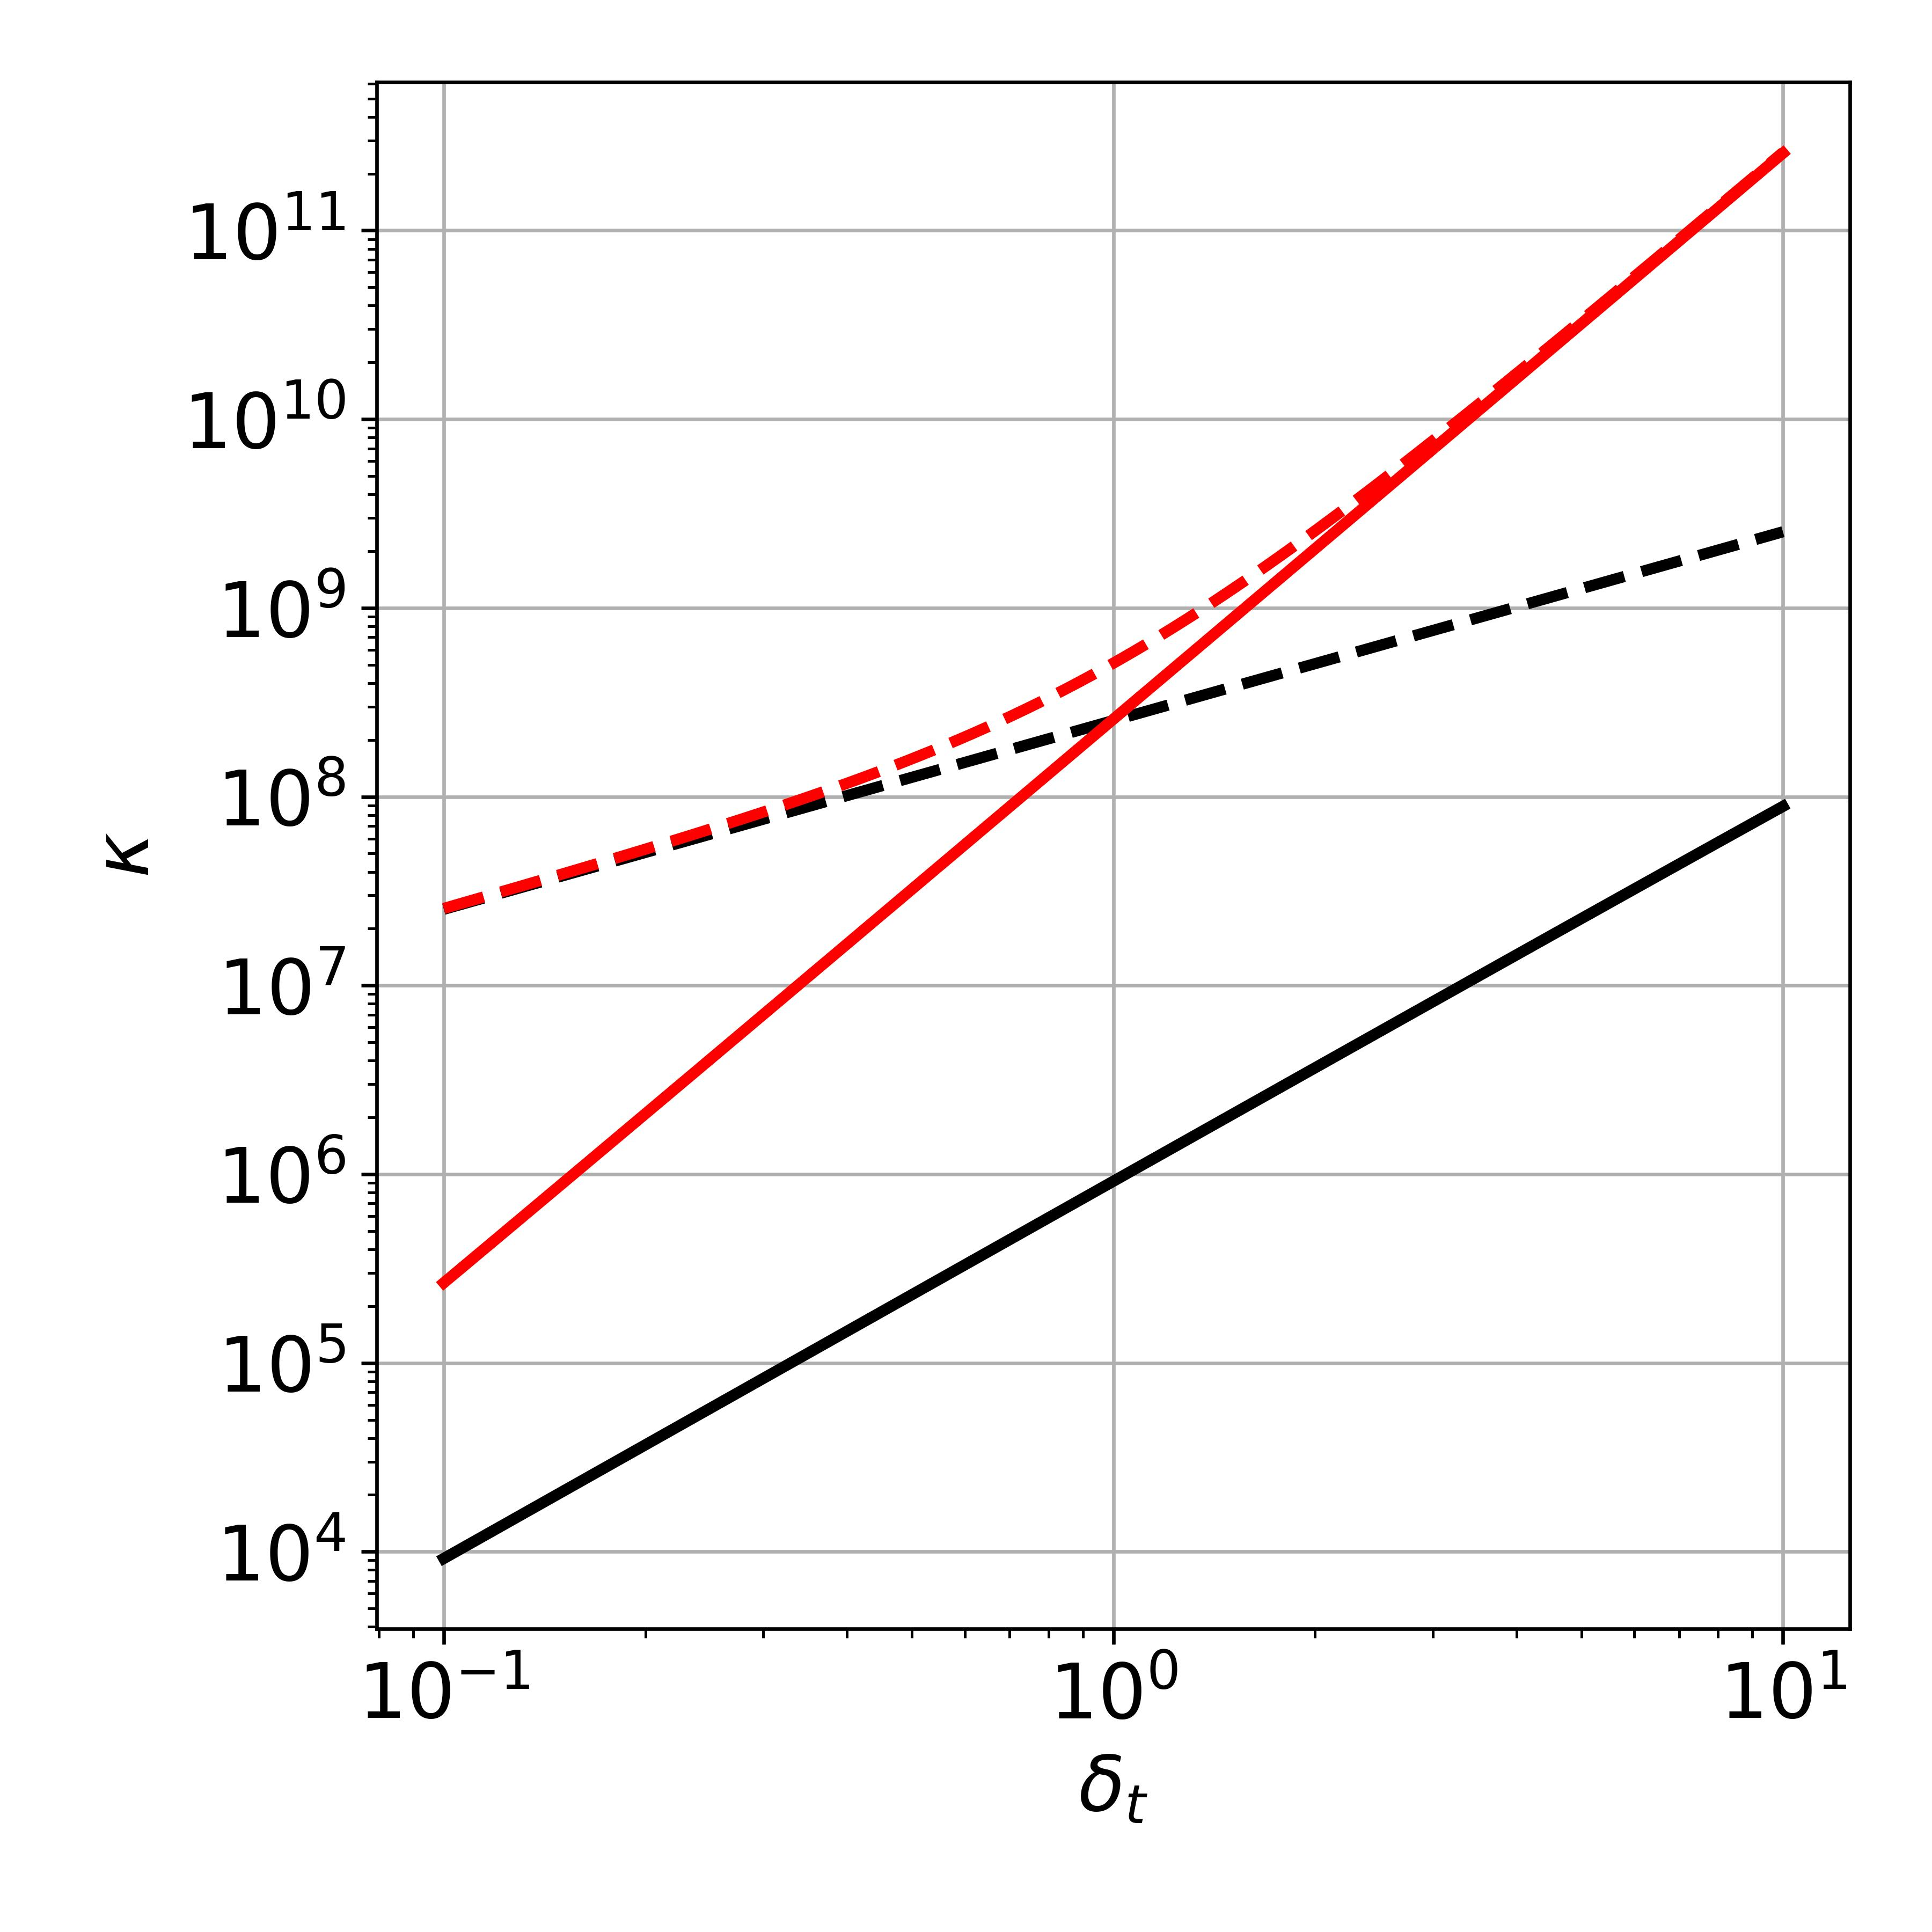
\includegraphics[width=1\textwidth]{schemes/conditionNumber_dt.jpg}
		\subcaption{Timestep size $\delta_t$}
		\label{fig:Impl_conditionNumber_dt}
	\end{subfigure}
	\begin{subfigure}[t]{0.30\textwidth}
		\centering
		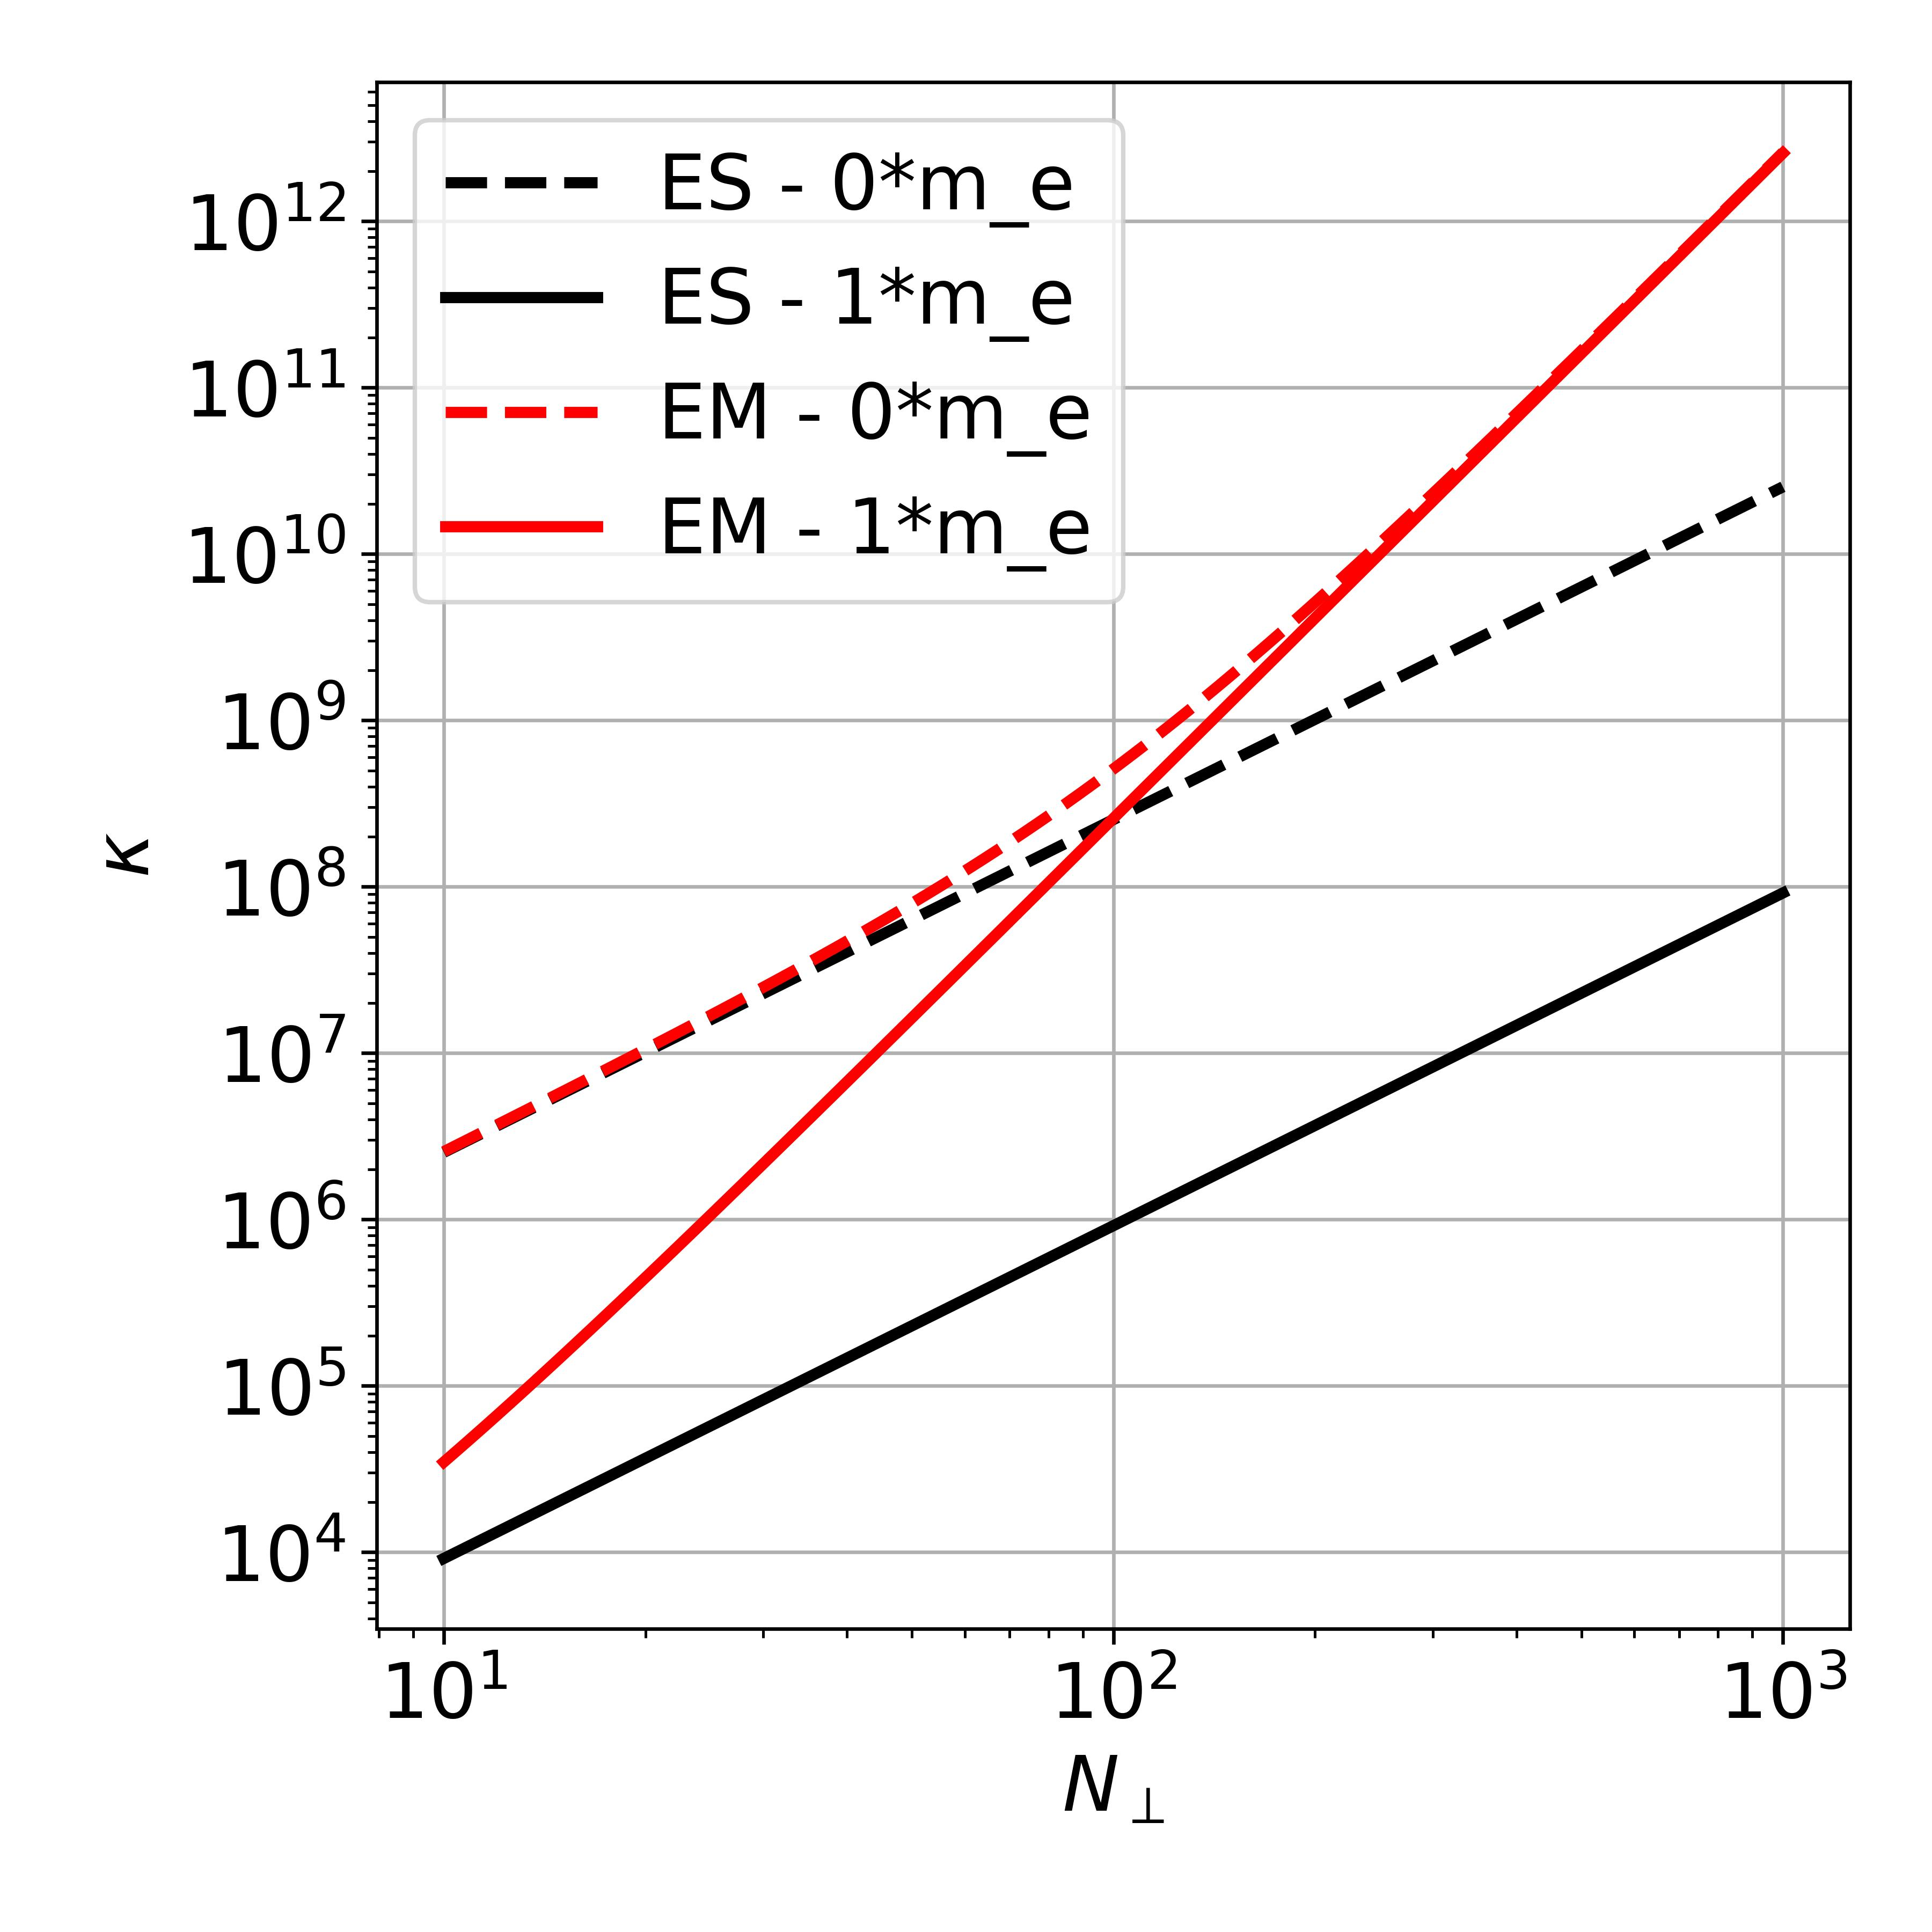
\includegraphics[width=1\textwidth]{schemes/conditionNumber_Nperp.jpg}
		\subcaption{Perpendicular \\ resolution $N_\perp$}
		\label{fig:Impl_conditionNumber_Nperp}
	\end{subfigure}
	\caption{Impact of different parameters on the condition number. Plasma parameters are taken as constant: $B=1$, $m_i = 2$, $n_e = n_i = 2$, $m_e = 5.5\cdot 10^{-4}$, $\beta_0 = 10^{-3}$, $\eta_\parallel = 10^{-6}$, $\delta_t = 1$ and $N_\perp = 100$. The parameters $\beta_0$ and $n_e$ are deliberately chosen large to ensure the validity of the positive-definiteness condition \ref{eq:Impl_conditionPositiveDefinite}. Black curves correspond to the electrostatic system, and red curves to the electromagnetic matrices, with full lines indicating electron inertia and dashed lines representing $m_e = 0$.}
	\label{fig:Impl_conditionNumber}
\end{figure}

Overall, electromagnetic models exhibit a higher condition number. In particular, at larger timestep sizes or higher perpendicular resolutions, $\kappa$ increases significantly due to the third and fourth exponents in the second term of Eq. \ref{eq:Impl_conditionNumberElectromagneticVorticitySystem}. However, electron inertia positively affects the condition number. This is especially evident as $\eta_\parallel$ approaches zero in Fig. \ref{fig:Impl_conditionNumber_eta}, where neglecting the electron mass results in a sharp increase in $\kappa$, while electron inertia allows for a stable, low $\kappa$. Similarly, for low timestep sizes and resolutions, $m_e$ improves the system, such that for lower ranges, the electromagnetic system with inertia performs better than the electrostatic system without inertia.

 




	\chapter{Verification and Validation}
\label{chap:VV}


\begin{chaptersummarybox}
	The implementation of the electromagnetic model is verified using the method of manufactured solutions on a three-dimensional, curved geometry with non-uniform meshing. Physical quantities are initialized as sinusoidal functions, and analytic source terms are computed to compensate for all time-independent terms in the equations, such that the simulation maintains a steady state. The root mean square difference between the initial state and the plasma state after one timestep is a appropriate to estimate the discretization error introduced by the implementation. First, the electromagnetic vorticity system with magnetic induction and electron inertia is verified. The complex geometry provides an advanced test for the correct implementation of fields on a staggered grid. The discrete parallel Laplacian operator developed for diffusion problems with flutter is tested separately on the parallel heat conduction term in the energy conservation equation. A resolution scan demonstrates that the error decreases with the square of the mesh size, consistent with the second-order schemes used for the tested stencils. \\
	
	The physical accuracy is validated on true 2D and 3D slabs with a uniform magnetic field against the linear behavior expected from the dispersion relation. The test setup is first checked on trivial advection and the electrostatic vorticity equation. Next, Alfvén waves are observed on a 2D slab with pure magnetic induction in the vorticity equation. The most comprehensive test is performed on a 3D slab with a (uniform) poloidal and toroidal magnetic field in a four-field model, where $A_\parallel$ and $j_\parallel$ evolve with a $\pi/2$ phase shift relative to $\Phi$ and $n_e$. A scan over the perpendicular wave motion exhibits the transition from Alfvén dynamics to thermal electron waves. The observed speeds are:
	
	\begin{align*}
		v_A &= \frac{B}{\sqrt{m_in_i\mu_0}} & v_{th,e} &= \sqrt{\frac{T_e}{m_e}}
	\end{align*} 
	
	where waves propagate at $v_A$ in the low $k_\perp$ limit and at $v_{th,e}$ in the upper $k_\perp$ limit.
	
\end{chaptersummarybox}

\newpage




The electromagnetic extension of the SOLEDGE3X framework required considerable modifications of the code. Before investigating new physics, it is wise to verify the correctness of the implementation and validate electromagnetic plasma behavior with it. In a first series of tests in Sec. \ref{sec:verification}, the implementation of the electromagnetic vorticity equation and the parallel diffusion with flutter are checked against analytic source term. The physical behavior is validated in Sec. \ref{sec:validation}, where test cases on 2D and 3D slabs with increasing model complexity are confronted to the expected linear behavior.


\section{Verification by the method of manufactured solutions}
\label{sec:verification}
To ensure the correctness of the newly implemented system with the magnetic vector potential $A_\parallel$, a test model has been set up with the method of manufactured solutions (MMS) \cite{ManufacturedSolution}. This allows to directly compare the numerical and analytic solutions and therefore validate the implementation and verify the order of convergence of the numerical operators. 

\subsection{Test set-up}
The MMS test model is a fraction of a torus with a circular cross-section with an inner radius of 0.48m, an outer radius of 2.72m and a simulated plasma edge width of 0.64m. An example of the 3D mesh geometry is shown in Fig. \ref{fig:MMSModelScheme}. To test the information exchange between zones in the model topology from Sec. \ref{ssec:impl_meshDecomposition}, each coordinate direction is split in two zones totaling to 8 zones.

\begin{figure}[H]
	\centering
	\begin{subfigure}[b]{0.4\textwidth}
		\centering
		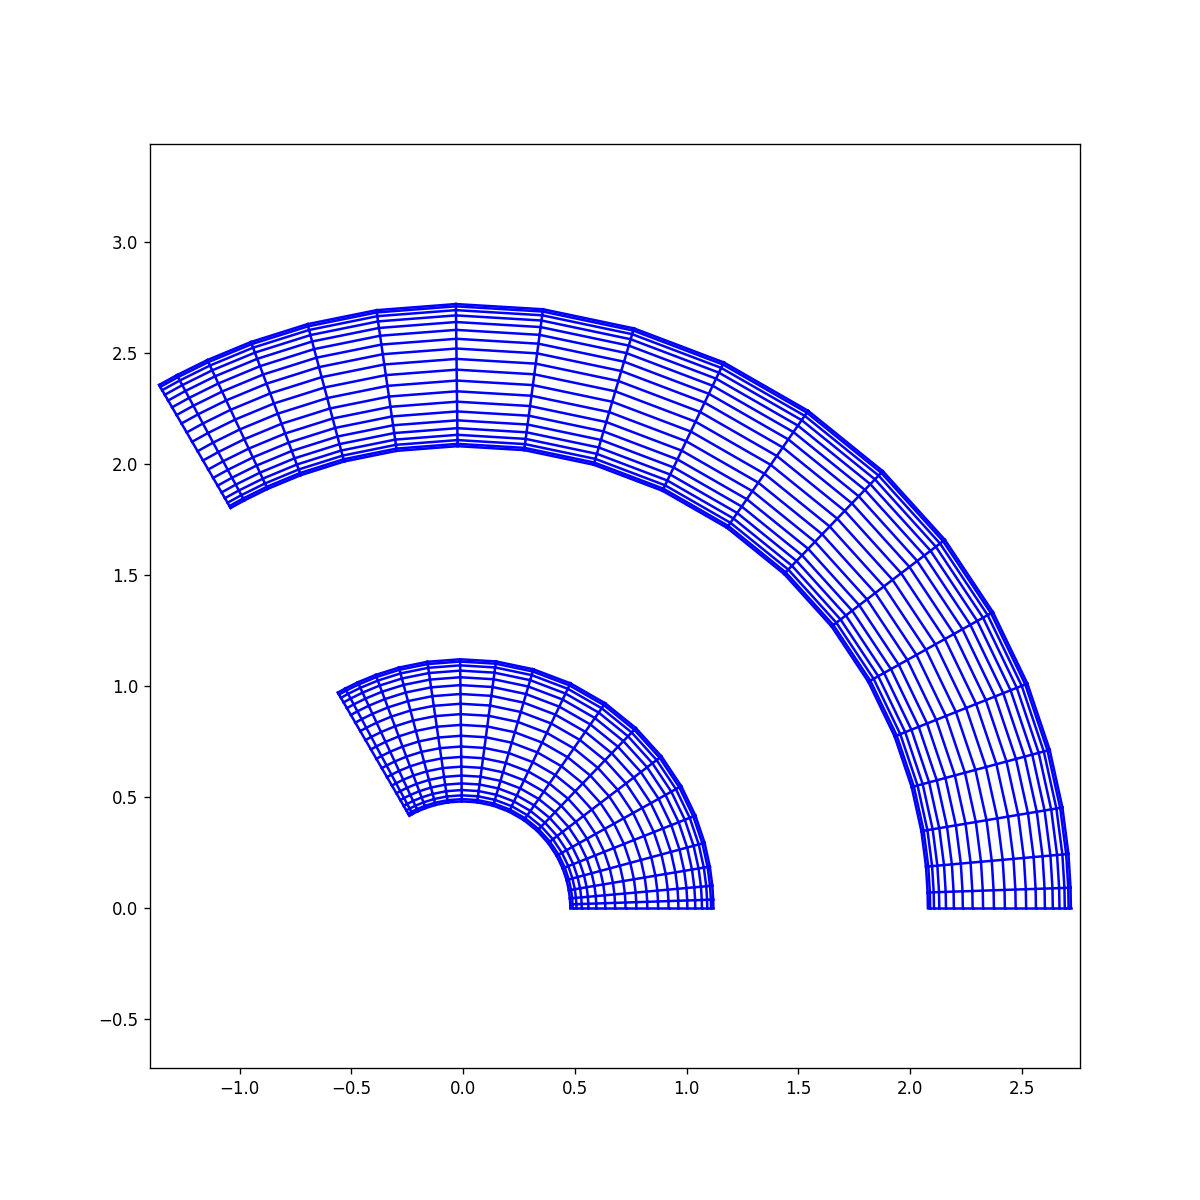
\includegraphics[width=1\textwidth]{schemes/torturedGrid_r_phi_view.png}
		\subcaption{Top view of the $\psi-\varphi$ plane \\ \textit{the two bands correspond to \\ the poloidal angles $0$ and $\pi$}}
		\label{fig:MMSModelTorturedTopView}
	\end{subfigure}
	\begin{subfigure}[b]{0.4\textwidth}
		\centering
		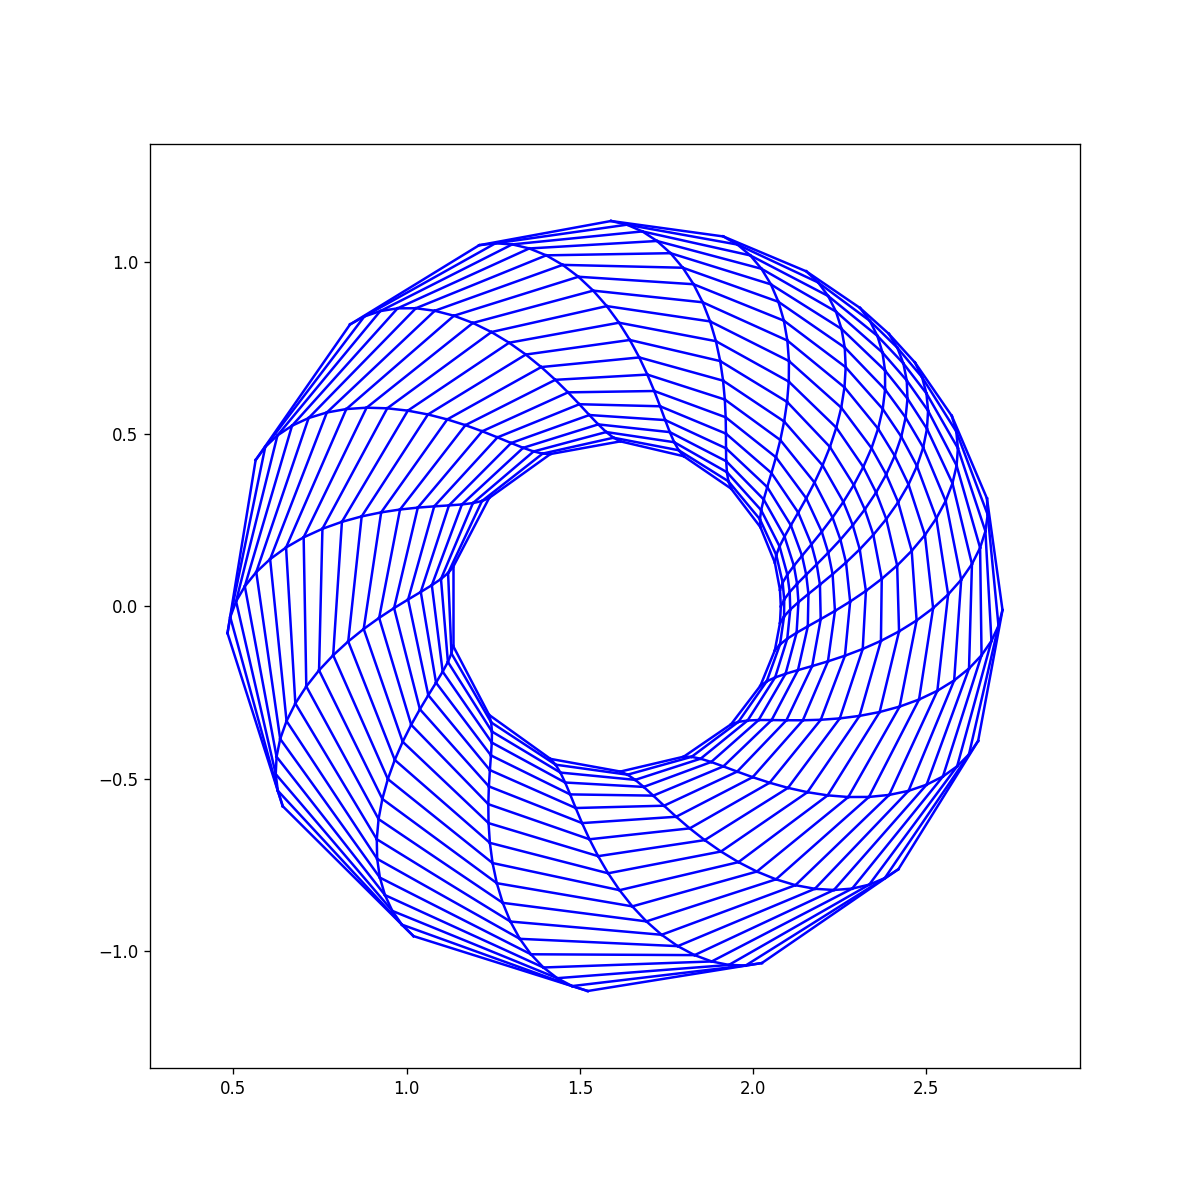
\includegraphics[width=1\textwidth]{schemes/torturedGrid_r_theta_view.png}
		\subcaption{View of a cross-section of the torus in the $\psi-\theta$ plane \\ \textit{The cross-section is at $\varphi=0$}}
		\label{fig:MMSModelTorturedCrossSection}
	\end{subfigure}	
	\caption[Distorted MMS mesh geometry with $N=20$ cells per dimension on a 3rd of a torus]{Distorted MMS mesh geometry with $N=20$ cells per dimension on a 3rd of a torus}
	\label{fig:MMSModelScheme}
\end{figure}

In the MMS geometry, $\psi$ denotes the radius of the tube and $R$ the radius of the entire torus. If $aR_0=1.6$ is the distance of the tube center to the torus center, we have:
$$  R = aR_0 + \psi\cdot\cos(\theta) $$
Together with the poloidal coordinate $\theta\in[0,2\pi]$ and the toroidal coordinate $\varphi\in[0,2\pi/N_{div}]$ where $1/N_{div}$ is the considered fraction of the torus, each point in the domain is uniquely described by the curvilinear coordinates $[\psi,\theta,\varphi]$. 
We can define some $\mathbf{P} = [X,Y,Z]^T$ in a cartesian basis of the 3D domain:

\begin{align*}
	X &= R\cos(\varphi) &  Y &= \psi\cdot\sin(\theta)  &  Z &= R\sin(\varphi)
\end{align*} 
In this setting, the basis vectors of the curvilinear coordinates from Sec. \ref{ssec:MetricCurvilinearCoordinates} can be calculated analytically. The covariant basis vectors are:
\begin{align*}
	\mathbf{e}_\psi &= \pdv{\mathbf{P}}{\psi} = \begin{bmatrix} \cos(\theta)\cos(\varphi) \\ \sin(\theta) \\ \cos(\theta)\sin(\varphi) \end{bmatrix} & \mathbf{e}_\theta &= \pdv{\mathbf{P}}{\theta} = \begin{bmatrix} -\psi\sin(\theta)\cos(\varphi) \\ \psi\cos(\theta) \\ -\psi\sin(\theta)\sin(\varphi) \end{bmatrix} & \mathbf{e}_\varphi &= \pdv{\mathbf{P}}{\varphi} = \begin{bmatrix} -Z \\ 0 \\ X \end{bmatrix}
\end{align*}
We can further calculate the metric coefficients:
$$ g_{ij} = \mathbf{e}_i\cdot\mathbf{e}_j
= \begin{bmatrix}
	1 & 0 & 0 \\ 0 & \psi^2 & 0 \\ 0 & 0 & R^2
\end{bmatrix} \qquad \text{and} \qquad J = \sqrt{\det[g_{ij}]} = \psi R$$
 
As generally required in SOLEDGE3X, the magnetic field is axisymmetric and thus does not depend on the toroidal coordinate $\varphi$. By construction, it only has a poloidal and a toroidal component but no radial component, which are given in Eq. \ref{eq:MMSMagneticField}.

\begin{equation}
	\label{eq:MMSMagneticField}
	\begin{cases}
		B_\theta = \frac{1}{aR}\Psi_0 & \text{poloidal magnetic field}  \\
		B_\varphi = \frac{R_0}{R}B_0 & \text{toroidal magnetic field}
	\end{cases}
\end{equation}

The magnetic field parameters are chosen such that the ratio of toroidal over poloidal magnetic field strength is $aR_0B_0/\Psi_0 = 12$. The conserved fields $n$, $\gamma$ and $T$ are pre-defined to sinusoidal functions on the grid for electrons and one ion species. 

\begin{align}
	n_\alpha &= 1  + 0.1 \cos(\theta)\cos(\frac{\varphi}{N_{div}})\sin(2\pi \frac{\psi-\psi_{min}}{\psi_{max} - \psi_{min}}) \\
	\gamma_\alpha &= 0.1 \cos(\theta)\cos(\frac{\varphi}{N_{div}})\sin(2\pi \frac{\psi-\psi_{min}}{\psi_{max} - \psi_{min}}) \\
	T_\alpha &= 1  + 0.1 \cos(\theta)\cos(\frac{\varphi}{N_{div}})\sin(2\pi \frac{\psi-\psi_{min}}{\psi_{max} - \psi_{min}})
\end{align}

Tests have been performed on various mesh geometries in the scope of SOLEDGE3X from a perfectly regular grid with equally spaced cells in all coordinate directions to the distorted mesh depicted above. As the program can be either executed in a 2D or 3D mode with adapted stencils and geometry calculations, MMS tests have been developed for both scenarios. \\


\subsection{Electromagnetic vorticity equation}

We are interested in the vorticity system on the electric potential $\Phi$ and the parallel magnetic vector potential $A_\parallel$. As free variables, they are set to a similar expression as the conserved fields: 
\begin{align}
	\Phi =& 1 + 0.1 \cos(\theta)\cos(\frac{\varphi}{N_{div}})\sin(2\pi \frac{\psi-\psi_{min}}{\psi_{max} - \psi_{min}}) \\
	A_\parallel =& 1 + 0.1 \cos(\theta)\cos(\frac{\varphi}{N_{div}})\sin(2\pi \frac{\psi-\psi_{min}}{\psi_{max} - \psi_{min}})
	\label{eq:MMSAnalyticFormPhiAPara}
\end{align}

The vorticity $\Omega$ and the parallel current $j_\parallel$ depend on the free fields and are initialized according to their definitions, where the derivatives on curvilinear coordinates can be calculated analytically with the metric theory discussed in Sec. \ref{ssec:MetricCurvilinearCoordinates} using Maple. 

\begin{align}
	\Omega =& \grad\cdot\left(\frac{m_i}{Z_iB^2}\grad_\perp[nT] + \frac{m_in_i}{B^2}\grad_\perp\Phi\right) \\ 
	j_\parallel =& \sigma_\parallel \left(-\grad_\parallel\Phi + T_e\grad_\parallel\log n_e + 1.71\grad_\parallel T_e\right)
\end{align}

Let us consider a slightly simplified version of the electromagnetic system in Eq. \ref{eq:S3X_vorticityEquation_FullElectromagnetic} without additional currents from the charge balance, advection terms of $j_\parallel$ or anomalous parallel diffusion. As the domain is fully periodic in parallel direction and no sheath boundaries are present to fix the potential, Dirichlet boundary conditions force the fields $\Phi$ and $A_\parallel$ to their initial values at the two radial boundaries and the system becomes uniquely solvable. 

\begin{equation}
	\begin{cases}
		\partial_t\Omega + \grad\cdot\sigma_\parallel \left(\grad_\parallel\Phi + \beta_0\partial_t A_\parallel + \frac{m_e}{n_e}\partial_t j_\parallel\right)\mathbf{b} &= \grad\cdot\sigma_\parallel\left(T_e\grad_\parallel\log n_e + 1.71\grad_\parallel T_e\right)\mathbf{b} + S^{MMS}_\Phi \\
		\grad\cdot\left(\grad_\perp A_\parallel\mathbf{b}\right) - \sigma_\parallel \left( \grad_\parallel \Phi + \beta_0\partial_t A_\parallel + \frac{m_e}{n_e}\partial_t j_\parallel\right)&= -\sigma_\parallel\left(T_e\grad_\parallel\log n_e + 1.71\grad_\parallel T_e\right) + S^{MMS}_{A_\parallel}
	\end{cases}
	\label{eq:MMSTestSystem}
\end{equation}

The MMS source terms $S^{MMS}_\Phi$ and $S^{MMS}_{A_\parallel}$ contain the analytic value of all time-independent terms in the respective line of the equation. The vorticity equation is then solved for one timestep, and if the implementation is correct, the system should maintain a steady state. One drawback of a steady state system is that time derivatives are always assumed to vanish and terms such as the perpendicular Laplacian of $\Phi$, $j_\parallel$ or the divergence of $A_\parallel$ are not confronted to their analytic form in the source term $S^{MMS}$. To catch these terms, it is important to consider the full expression of the vorticity $\Omega$ as its initial value contains the analytic terms. \\

The system is run for exactly one timestep where only the discretization error modifies the values of the fields. This allows to compare a numerical and an analytic form of the vorticity and confront all terms in Eq. \ref{eq:MMSTestSystem} to their expected values. To measure the error, we calculate the root mean square error $\epsilon_d$ of the solution $X$ to the initial, analytic field $X_{ana}$:

\begin{equation}
	\epsilon_d = \sqrt{\frac{1}{N}\sum\left(X-X_{ana}\right)^2}
\end{equation}

where we sum the residual for each point in the domain excluding the imposed Dirichlet boundaries. To quantify the discretization error, we run the same simulation on increasingly high spatial resolutions and compare the error to the coarsest case. Second order stencils were used in the implementation, so we expect that the error reduces by a factor 4 when the resolution is doubled in a direction. The errors for the 2D and 3D implementations of the vorticity system are shown in Fig. \ref{fig:MMSTorturedVortAParaConvergence}. The dashed line indicates the ideal slope of second order convergence, and we observe that the errors decrease with a close match to the expected convergence as the resolution increases. This verifies the correct implementation of the vorticity equation in the SOLEDGE3X framework. 

\begin{figure}[H]
	\centering
	\begin{subfigure}[b]{0.49\textwidth}
		\centering
		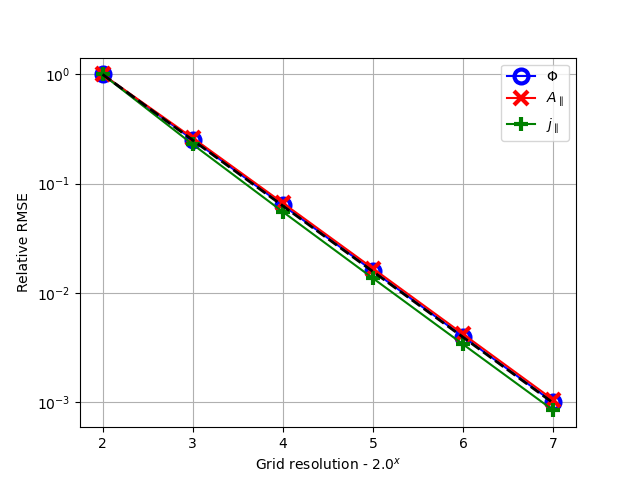
\includegraphics[width=1\textwidth]{schemes/err_rel_vortAParaJParaSystem_grid1_2D.png}
		\subcaption{2D system}
		\label{fig:MMSTorturedVortAPara2DConvergence}
	\end{subfigure}
	\begin{subfigure}[b]{0.49\textwidth}
		\centering
		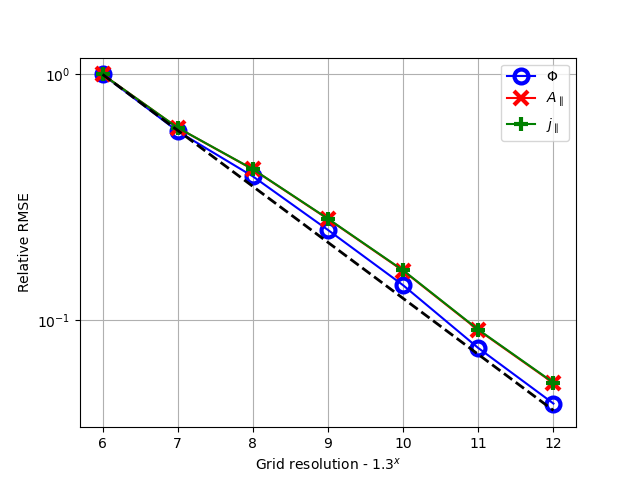
\includegraphics[width=1\textwidth]{schemes/err_rel_vortAParaJParaSystem_grid2_3D.png}
		\subcaption{3D system}
		\label{fig:MMSTorturedVortAPara3DConvergence}
	\end{subfigure}
	\caption[Relative error between the initial plasma and the solution after one timestep for the electromagnetic vorticity system]{Relative error between the initial plasma and the solution after one timestep for the electromagnetic vorticity system. The $x$-axis indicates the number of points per zone in each direction, the total number of points is thus $N_{tot}^{3D} = 8\cdot X^3$ (resp. $N_{tot}^{2D} = 4\cdot X^2$). The dashed lines indicate the slope of the ideal 2nd order convergence}
	\label{fig:MMSTorturedVortAParaConvergence}
\end{figure}


\subsection{Parallel heat diffusion with flutter}

A second row of tests affects is dedicated to the correct implementation of the radial magnetic field that originates from flutter. The most critical new code component in that regard are the implicit parallel diffusion equations for heat and viscosity. For that purpose, we consider a very reduced energy conservation equation for electrons and ions, that effectively only remains with the parallel heat conduction from the Spitzer-Härm model. 

\begin{align}
	\partial_t \left( \frac{3}{2} n_e T_e                                          \right) &= \vec{\nabla}\cdot\left(\kappa_0 T_e^{5/2} \nabla_\parallel T_e \vec{b}\right) + S_{T_e}^{MMS} \\
	\partial_t \left( \frac{3}{2} n_i T_i + \frac{1}{2} \frac{m_i}{n_i} \gamma_i^2 \right) &= \vec{\nabla}\cdot\left(\kappa_0 T_i^{5/2} \nabla_\parallel T_i \vec{b}\right) + S_{T_i}^{MMS} 
\end{align}

The simulation set-up follows the same model as for the test on the vorticity equation as the sources are calculated analytically to maintain a steady-state and radial Dirichlet boundaries are imposed. The main novelty here is the addition of a radial component in the magnetic field, whose contravariant form is given by:

\begin{equation}
	b^\psi =\frac{ 0.01}{B_{eq}} \cos(\theta)\cos(\frac{\varphi}{N_{div}})\sin(2\pi \frac{\psi-\psi_{min}}{\psi_{max} - \psi_{min}})
\end{equation}

To be as realistic as possible with the real flutter, it is scaled by the magnitude of the equilibrium field (and not the total field) and takes both positive and negative values to adequately address the fluctuating nature of flutter. It allows to test the new 3D parallel diffusion operator from Sec. \ref{ssec:impl_3DGunter} and challenges it to the crucial case where $b^\psi$ tends to zero. The simulation was only run on the 3D MMS mesh, as it is the only effectively relevant use case. The root mean square error is shown in Fig. \ref{fig:MMSTorturedFlutterDiffParaConvergence} for both temperatures, and we can still observe a satisfying agreement with the expected second order convergence.

\begin{figure}[H]
	\centering
	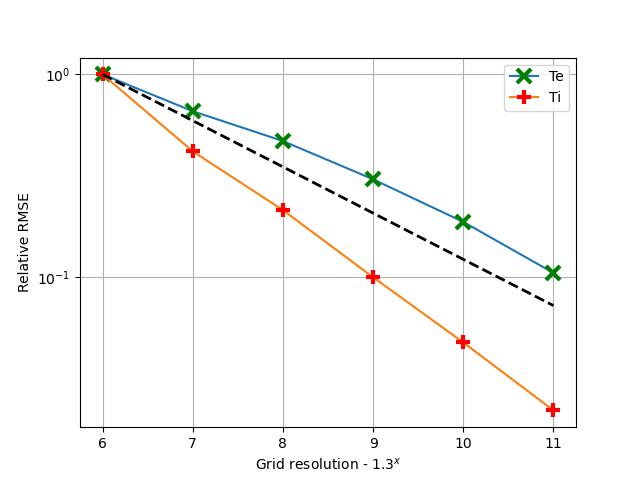
\includegraphics[width=0.6\textwidth]{schemes/err_rel_paradif_Brad_grid2_3D.png}
	\caption[Relative error between the initial plasma and the solution after one timestep for the parallel 3D heat diffusion system with flutter]{Relative error between the initial plasma and the solution after one timestep for the parallel 3D heat diffusion system with flutter. The $x$-axis indicates the number of points per zone in each direction, the total number of points is thus $N_{tot}^{3D} = 8\cdot X^3$. The dashed lines indicate the slope of the ideal 2nd order convergence}
	\label{fig:MMSTorturedFlutterDiffParaConvergence}
\end{figure}




\section{Validation on linear systems}
\label{sec:validation}
The MMS verification confirmed the correctness of the implementation. A more integrative, physics-based validation of the electromagnetic model is proposed here to recover the linear behavior in ideal slab configurations. We first verify the general test framework on the transport term and the electrostatic vorticity equation before investigating Alfvén dynamics and the interaction with electron inertia effects.


\subsection{Pure advection}
A first step to validate the correct physical behaviour of the simulation and to test the general validation framework would be to investigate the plasma advection equations. We can hence define parallel and perpendicular wavenumbers $k_\parallel$ and $k_\perp$ that  For this objective we set up a simplistic plasma model on a rectangular 2D SLAB topology, where magnetic field is uniform in poloidal Z direction. Periodic boundary conditions in all directions allow to properly observe wave propagation without any inference at the domain boundaries. In an isothermal hydrogen plasma without source terms and drifts, the governing equations then simplify to:

\begin{align}
	\partial_t n_i + \grad\cdot\left(n_i\mathbf{u}_i\right) &= 0 \label{eq:AdvectionLinearAnalysis_ionMass} \\
	\partial_t \left(m_in_iu_\parallel\right) + \grad\cdot\left(m_in_iu_\parallel u_i\right) &= -2T_e\grad_\parallel n_e \label{eq:AdvectionLinearAnalysis_parallelMomentumBalance}
\end{align}

In this simple plasma, only the density and the velocity evolve over time and depend on each other. The electric potential $\Phi$ can also be computed and observed, but it does not interfere with the system because the parallel electric field in the momentum balance Eq. \ref{eq:AdvectionLinearAnalysis_parallelMomentumBalance} is calculated from the electron pressure gradient $E_\parallel = (\grad_\parallel p_e + R_e) / n_e$. \\

To perform the linear analysis of the system, we assume that field variables such as the velocity or density respect some Fourier solution as sum of several wave modes with respective amplitudes $\tilde{X}_{\omega,k_\perp,k_\parallel}$:
\begin{equation}
	 X = \bar{X} + \hat{X} = X_0 + \sum\tilde{X}_{\omega,k_\perp,k_\parallel}e^{i(-\omega t + k_\perp \psi + k_\parallel \theta)} \label{eq:FourierModeSolution}
\end{equation}

Since we do not consider any drifts the radial component $u_\psi$ of the velocity vector vanishes. Further, the mean density is $\bar{n}=n_0$ while the mean velocity $\bar{u}_\theta$ is zero. Because we are only interested in a first order approximation of the solution, we neglect all higher-order mixed fluctuating terms. Thus, Eq. \ref{eq:AdvectionLinearAnalysis_ionMass} and Eq. \ref{eq:AdvectionLinearAnalysis_parallelMomentumBalance} transform to:

\begin{align*}
	&&-i\omega\hat{n} + i\bar{n}k_\parallel\hat{u}_\theta + i\bar{u}_\theta k_\parallel\hat{n} &= 0 &\Leftrightarrow&& \hat{u}_\theta &= \frac{\omega}{n_0k_\parallel}\hat{n} \\
	&& -i\omega m_i \left(\bar{n}\hat{u}_\theta + \bar{u}_\theta\hat{n}\right) + im_ik_\parallel\left(2\bar{n}\bar{u}_\theta\hat{u}_\theta + \bar{u}_\theta^2\hat{n}\right) &= -2iT k_\parallel\hat{n}	&\Leftrightarrow&&  \hat{u}_\theta &= \frac{2T k_\parallel}{m_in_0\omega}\hat{n}
\end{align*}

Both are combined to obtain a dispersion relation for the frequency $\omega$:
\begin{align}
	&& \frac{\omega}{n_0k_\parallel} &= \frac{2T k_\parallel}{m_in_0\omega} 
	&\Leftrightarrow&& \omega &= \pm\sqrt{\frac{2T}{m}}k_\parallel \label{eq:AdvectionLinearAnalysis_dispersionRelation}
\end{align}

It is apparent that both solutions for $\omega$ are real therefore non-decaying waves traveling with the speed of sound $c_s = \sqrt{2T/m}$ appear. The perpendicular wave mode does not contribute to the equation so a 1D system along the poloidal axis is sufficient to simulate the behaviour. Both the electron and the ion density are initialized with one sinusoidal perturbation and Fig. \ref{fig:AdvectionSLAB_densityEvolution} shows their evolution. The electron velocity in Fig. \ref{fig:AdvectionSLAB_velocityEvolution} responds to this initial excitation with a shifted standing wave with same frequency. 

\begin{figure}[H]
	\centering
	\begin{subfigure}[b]{0.32\textwidth}
		\centering
		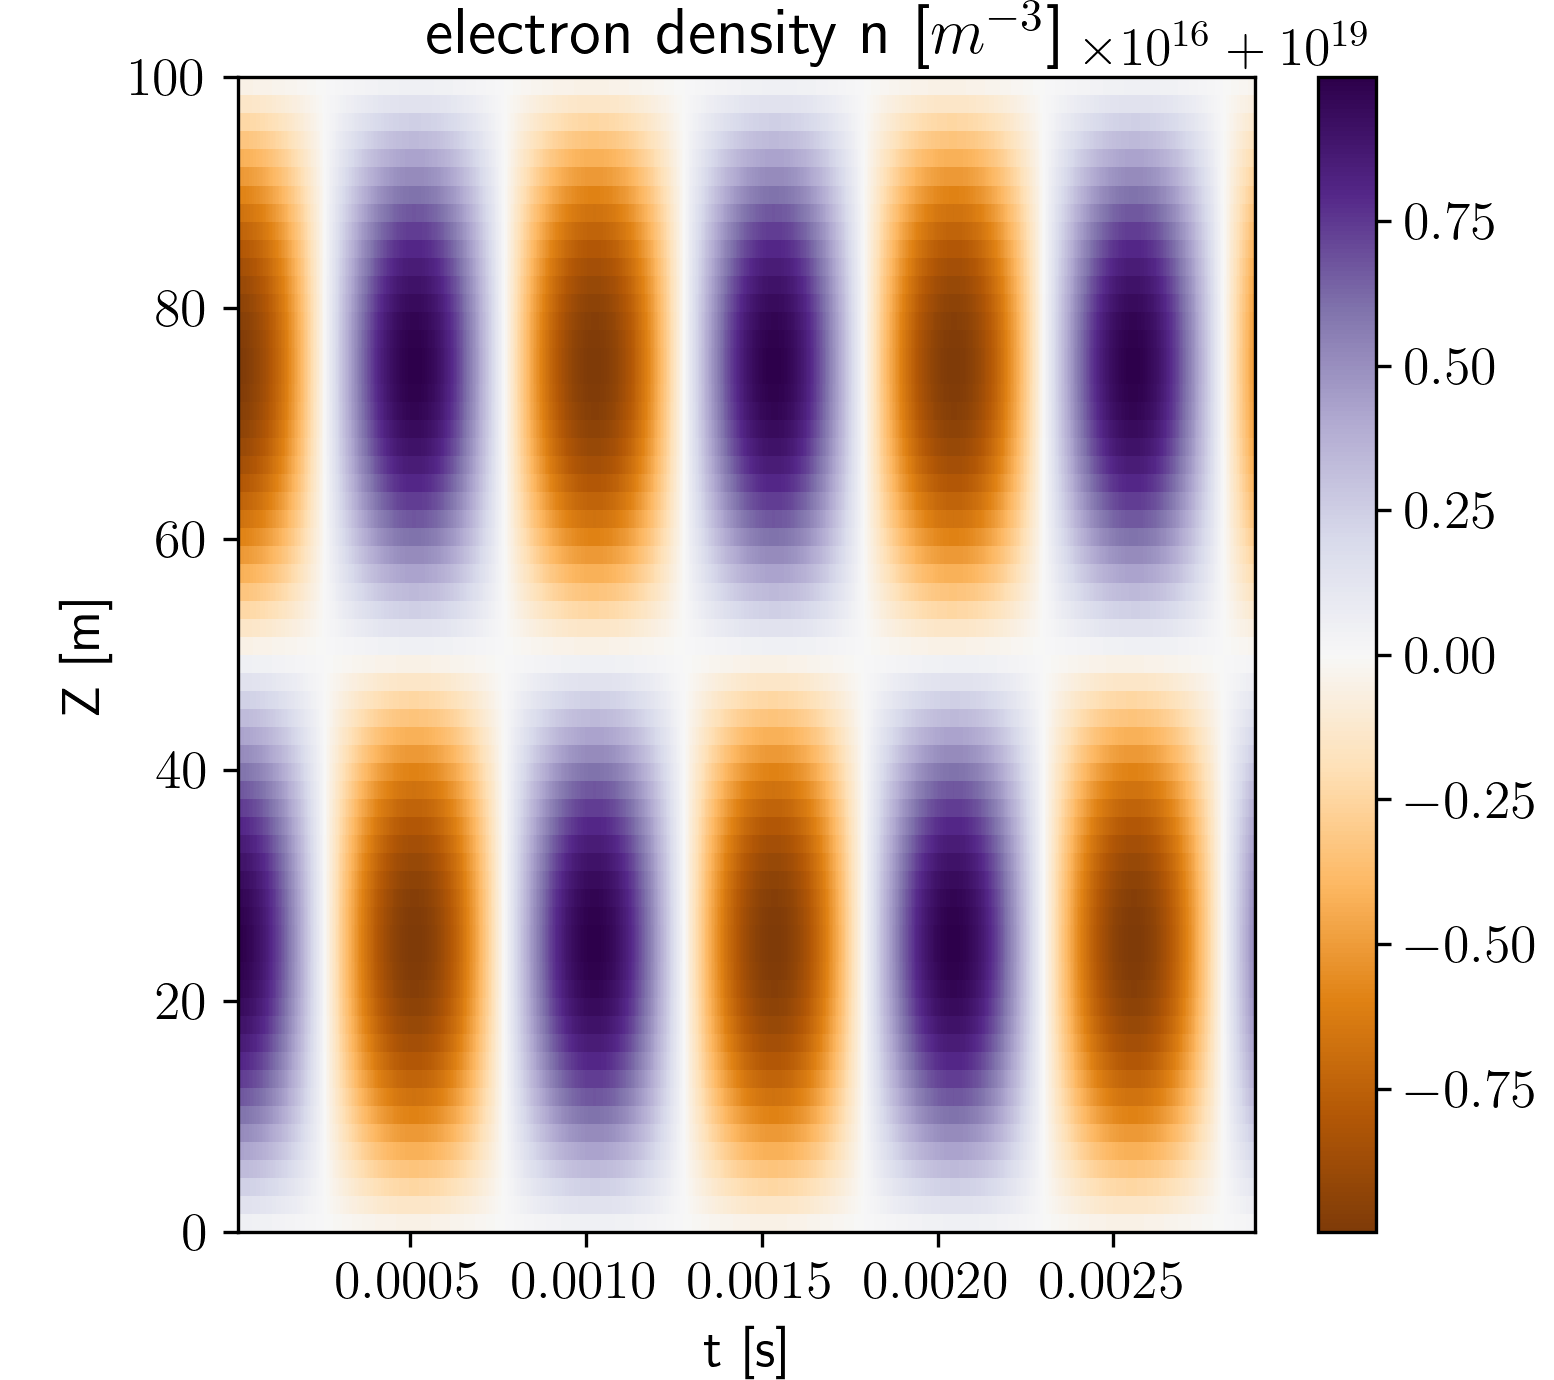
\includegraphics[width=1\textwidth]{schemes/AdvectionSLAB_1D_timeplot_ne.png}
		\subcaption{Evolution of the density \\ \ }
		\label{fig:AdvectionSLAB_densityEvolution}
	\end{subfigure}
	\begin{subfigure}[b]{0.32\textwidth}
		\centering
		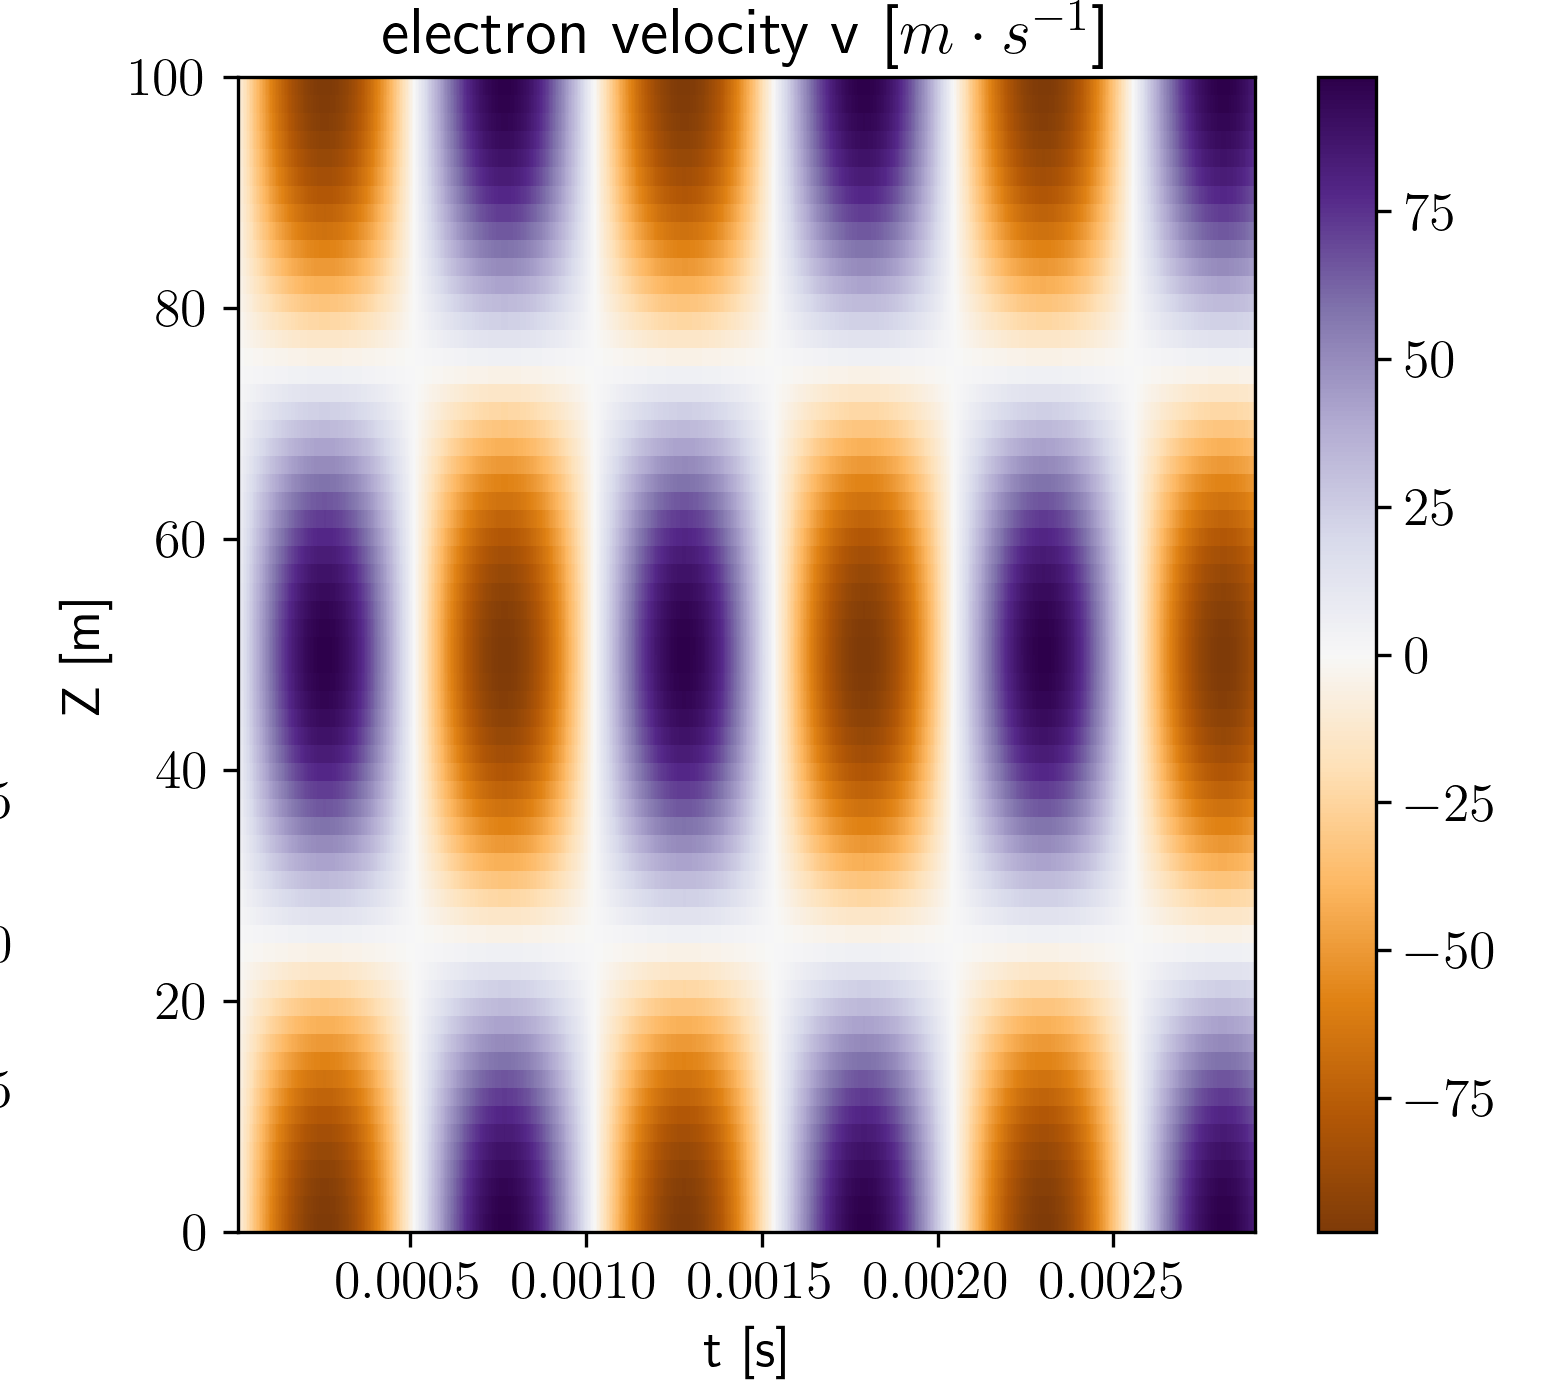
\includegraphics[width=1\textwidth]{schemes/AdvectionSLAB_1D_timeplot_ve.png}
		\subcaption{Evolution of the velocity \\ \ }
		\label{fig:AdvectionSLAB_velocityEvolution}
	\end{subfigure}
	\begin{subfigure}[b]{0.32\textwidth}
		\centering
		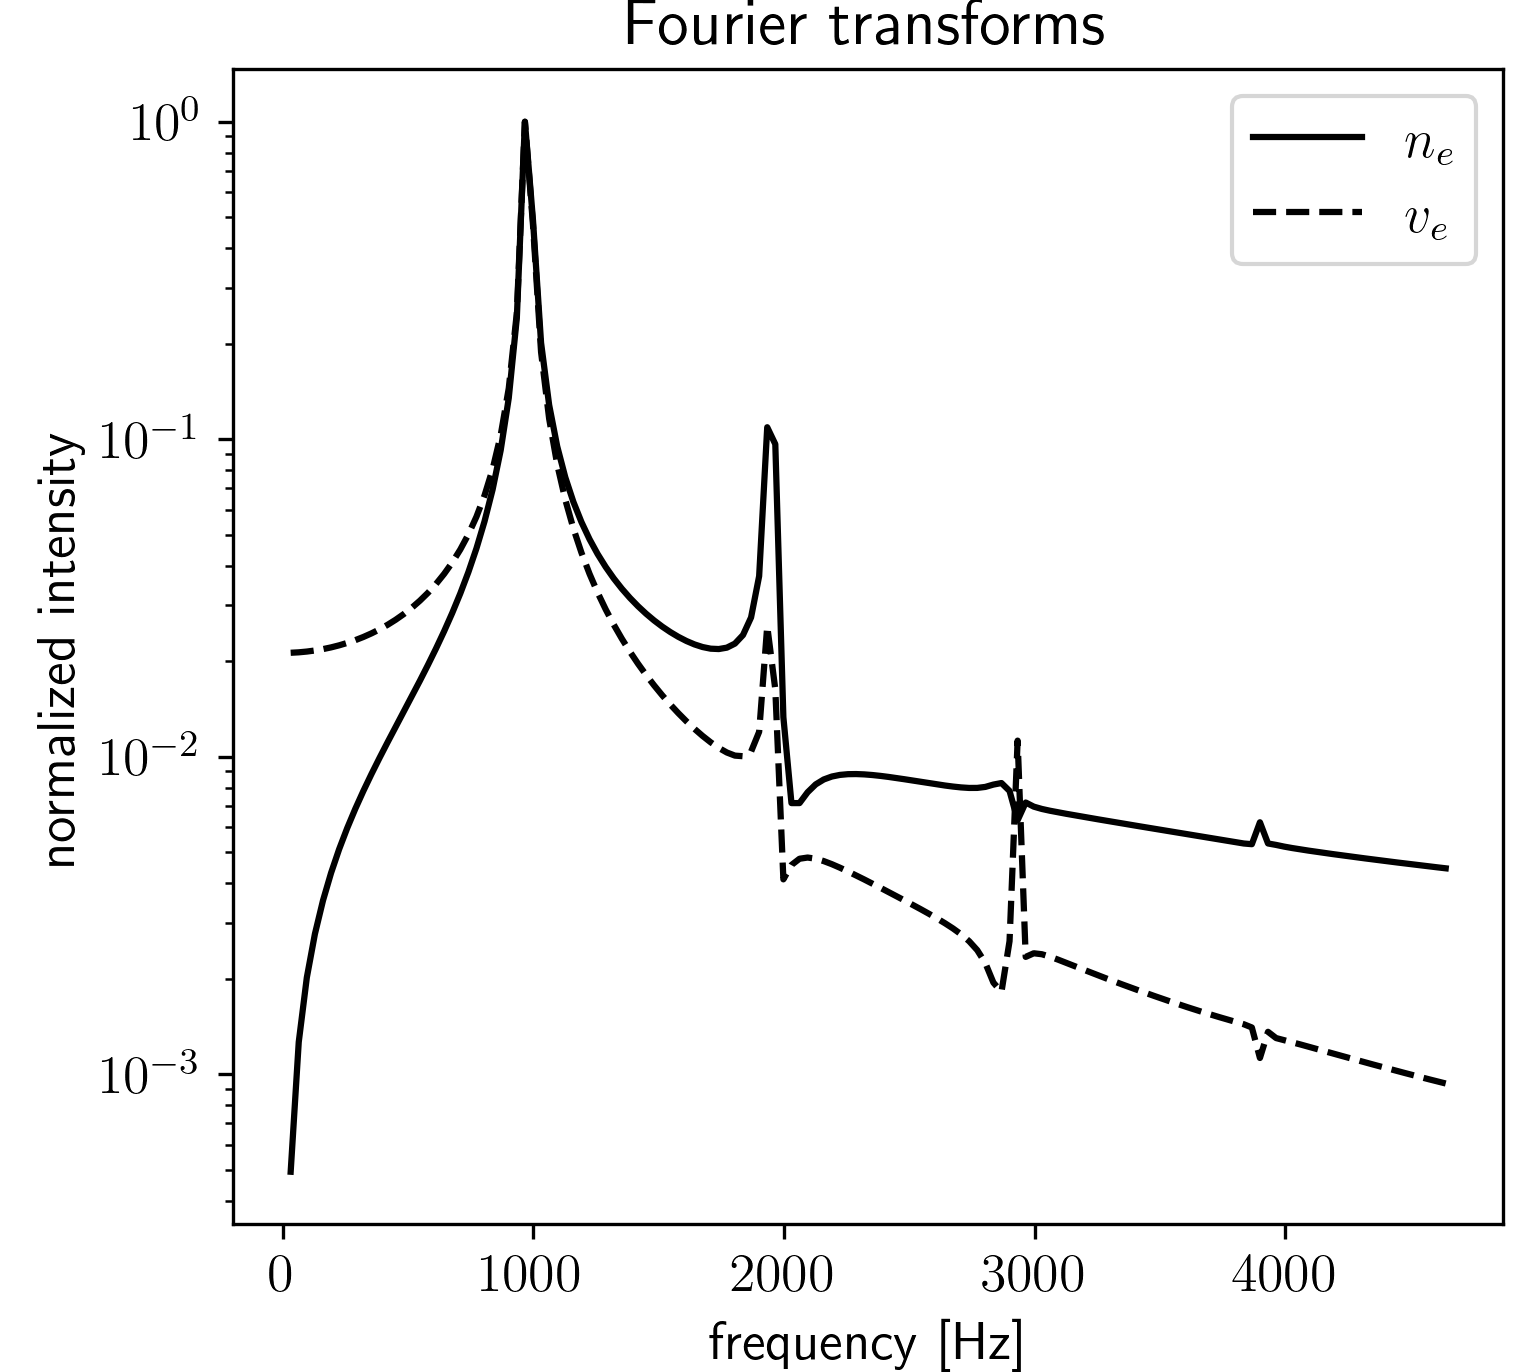
\includegraphics[width=1\textwidth]{schemes/AdvectionSLAB_FFT.png}
		\subcaption{time Fourier transform of the density and velocity}
		\label{fig:AdvectionSLAB_FFT}
	\end{subfigure}
	\caption[Evolution of the 1D SLAB system with 64 cells in poloidal direction over 10000 timesteps with the RK4 scheme]{Evolution of the 1D SLAB system with 64 cells in poloidal direction over 10000 timesteps with the RK4 scheme. For a better readability only parts of the graphs are represented}
	\label{fig:AdvectionSLAB}
\end{figure}

The system is initialized with one wavemode along the "poloidal" length of $L=100$m so the wavenumber here is $k_\parallel = 2\pi / L \approx 0.0628$. The plasma temperature is kept constant at $T = 100$eV and the mass of a deuterium atom equals to $m_i \approx 3.34\cdot 10^{-27}$kg, so we can expect a system frequency of $\omega\approx 978$Hz from the dispersion relation in Eq. \ref{eq:AdvectionLinearAnalysis_dispersionRelation}. This corresponds precisely to the main frequency peak in Fig. \ref{fig:AdvectionSLAB_FFT} and thus acoustic waves appear in the system as expected. The smaller peaks at higher frequency modes are however not physical and are likely due to numerical noise as their appearance highly depends on the spatial and temporal resolution and their intensity increases for longer simulations. 


\subsection{Electrostatic vorticity equation}
Before plunging into the vorticity equation with $A_\parallel$ it may be interesting to discuss whether the correct behaviour is actually observed in the original electrostatic implementation. For that we reduce the system to the bare minimum set of equations that involve the electric potential $\Phi$. Neglecting all kind of transport equations and source phenomena remains the following simple equation on $\Phi$: \\
\begin{equation}
		\partial_t\grad\cdot\left[\frac{m_in_i}{B^2}\grad_\perp\Phi\right] = -\grad\cdot\sigma_\parallel\grad_\parallel\Phi \label{eq:AdvectionSLAB_PHI}
\end{equation}

whose simple dispersion relation reads, assuming that $k_\perp \ne 0$:
\begin{align}
	\omega &= -\frac{B^2\sigma_\parallel}{m_in_i}\frac{k_\parallel^2}{k_\perp^2}i &\Rightarrow&& \lambda &= \frac{B^2\sigma_\parallel}{m_in_i}\frac{k_\parallel^2}{k_\perp^2}
\label{eq:AdvectionSLAB_dispersionRelation}
\end{align}

As $\omega$ is a pure negative complex number, we do not expect any oscillations but an exponential decay of the solution. All points in the domain decay with 
\begin{align}
	\Phi(t) = \Phi_0 e^{-\lambda t} + C \label{eq:electrostaticSLABdecay}
\end{align} 
where the decay rate $\lambda$ is the negative imaginary part of $\omega$ and $\Phi_0$ relates to the initial distribution of the electric potential.

The time integration of this system can only be performed by solving the implicit system because there is no direct expression for the time derivative of $\Phi$. Further, the electric potential $\Phi$ appears only in perpendicular and parallel Laplacian operators. Together with the periodic boundary conditions in all directions, one degree of freedom remains and the solution of $\Phi$ can only be calculated up to a constant $C$. To make the system invertible, it is thus necessary to add some term to the system. One simple approach is to fix (or ground) $\Phi$ to a set value $\Phi^G$ at one point $[i_\psi^G, i_\theta^G]$ in the domain. This defines the free parameter $C$ and $\Phi(t)$ at all points converges to $\Phi^G$. 

\begin{figure}[H]
	\centering
	\begin{subfigure}[b]{0.34\textwidth}
		\centering
		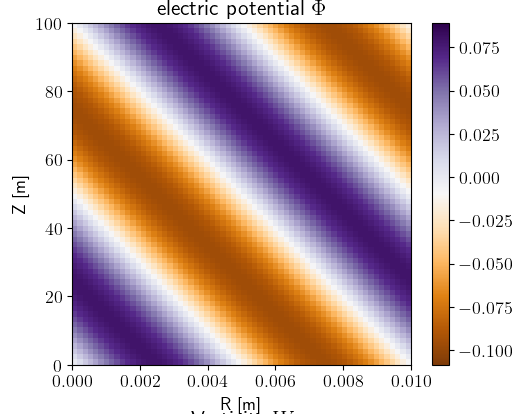
\includegraphics[width=1.\textwidth]{schemes/electrostaticSLAB_1_Phi.png}
		\subcaption{Initial $\Phi(\psi,\theta)$ \\ \ }
		\label{fig:electrostaticSLAB_initialProfile_PHI}
	\end{subfigure}
	\begin{subfigure}[b]{0.34\textwidth}
		\centering
		\includegraphics[width=1.\textwidth]{schemes/electrostaticSLAB_35_Phi.png}
		\subcaption{$\Phi(\psi,\theta)$ after 350 timesteps \\ \ }
		\label{fig:electrostaticSLAB_endProfile_PHI}
	\end{subfigure}
	\begin{subfigure}[b]{0.30\textwidth}
		\centering
		\includegraphics[width=0.95\textwidth]{schemes/Electrostatic_analysis_different_k_para_k_perp.png}
		\subcaption{Estimated decay rates for different wavemodes}
		\label{fig:electrostaticSLAB_decayRateFit}
	\end{subfigure}
	\caption[Evolution of the 2D electrostatic SLAB system with 64 cells in radial and poloidal direction over 10000 timesteps with the implicit Euler scheme]{Evolution of the 2D electrostatic SLAB system with 64 cells in radial and poloidal direction over 10000 timesteps with the implicit Euler scheme. The system is grounded at the center of the domain to $\Phi^G = 0$V.}
	\label{fig:electrostaticSLAB}
\end{figure}

The uniform decay can be clearly seen between Fig. \ref{fig:electrostaticSLAB_initialProfile_PHI} and Fig. \ref{fig:electrostaticSLAB_endProfile_PHI}. It remains to investigate whether the observed attenuation matches the expected decay rate $\lambda$. A Fourier transformation as to determine oscillatory modes for the standing acoustic waves in the previous section is not of great help here, instead we use a non-linear least squares to fit the time evolution of $\Phi(t)$ at an arbitrary point in the domain except the grounded point. We fit the parameters $\Phi_0$, $\lambda$ and $C$ from Eq. \ref{eq:electrostaticSLABdecay} to the simulation data and compare the hence estimated $\lambda$ to the theoretical decay rate for the given initial wave. Fig. \ref{fig:electrostaticSLAB_decayRateFit} shows that there is a strong agreement between the theoretical and fitted decay rates for a large array of domain configurations. The wavenumbers $k_\parallel$ and $k_\perp$ were modified by changing the poloidal respectively the radial size of the domain with always the first wave mode spanning the entire domain. We can safely claim that the original electrostatic implementation produces the expected physical behaviour.

\subsection{Electromagnetic vorticity equation}
While acoustic waves are characteristic for a physical medium, Alfvén waves dominate oscillations of ions within a magnetic field. The motion occurs in direction of the magnetic field lines where the ion mass accounts for the inertia and the magnetic field tension for the restoring wave force. The Alfvén wave group velocity for a species $i$ is given by:

\begin{equation}
	v_A = \frac{B}{\sqrt{m_in_i\mu_0}} \label{eq:AlfvenGroupVelocity}
\end{equation}

With the new parallel magnetic vector potential $A_\parallel$ into the vorticity Eq. \ref{eq:vorticityEquation_electromagnetic} Alfvén waves should appear in the simulation and the aim of this section is to prove their existence. We follow the same approach as in the previous section for the electrostatic case and reduce the system to the strict necessary minimum and keep following equations: 

\begin{align}
	\partial_t\grad\cdot\left[\frac{m_in_i}{B^2}\grad_\perp\Phi\right] &= \grad\cdot\sigma_\parallel\left(-\grad_\parallel\Phi-\partial_tA_\parallel\right) \label{eq:electromagneticSLAB_PHI} \\
	\Delta_{\perp}A_\parallel &= -\mu_0\sigma_\parallel\left(-\grad_\parallel\Phi-\partial_tA_\parallel\right) \label{eq:electromagneticSLAB_APara}
\end{align}

We ignore any kind of advection phenomena thus all densities $n_{i/e}$ and temperatures $T_{i/e}$ keep their initial uniform distributions their gradients vanish. If we perform the linear analysis of the remaining system we get following relation for Eq. \ref{eq:electromagneticSLAB_PHI}:
\begin{align*}
	&&i\frac{m_in_i}{B^2}k_\perp^2\omega\hat{\Phi} &= \sigma_\parallel k_\parallel^2\hat{\Phi}-\sigma_\parallel k_\parallel\omega\hat{A}_\parallel \\
	&\Leftrightarrow& \hat{A}_\parallel &= \left(\frac{k_\parallel}{\omega} - i\frac{m_in_ik_\perp^2}{\sigma_\parallel B^2k_\parallel}\right)\hat{\Phi}
\end{align*}

and for Eq. \ref{eq:electromagneticSLAB_APara}:
\begin{align*}
	&&-k_\perp^2\hat{A}_\parallel &= i\mu_0\sigma_\parallel k_\parallel\hat{\Phi} - i\mu_0\sigma_\parallel\omega\hat{A}_\parallel \\
	&\Leftrightarrow&\hat{A}_\parallel &= \frac{\mu_0\sigma_\parallel k_\parallel}{\mu_0\sigma_\parallel\omega + i k_\perp^2}\hat{\Phi}
\end{align*}

If we combine both expressions we can relate the frequency to the parallel and perpendicular wave modes:
\begin{align}
	&& \frac{k_\parallel}{\omega} - i\frac{m_in_ik_\perp^2}{\sigma_\parallel B^2k_\parallel} &= \frac{\mu_0\sigma_\parallel k_\parallel}{\mu_0\sigma_\parallel\omega + i k_\perp^2} \nonumber \\
	&\Leftrightarrow& i\frac{m_in_ik_\perp^2\omega}{\sigma_\parallel B^2k_\parallel^2} &= 1- \frac{\mu_0\sigma_\parallel\omega}{\mu_0\sigma_\parallel\omega + i k_\perp^2} \nonumber \\
	&\Leftrightarrow& \omega^2 + i\frac{k_\perp^2\omega}{\mu_0\sigma_\parallel} &= \frac{B^2}{m_in_i\mu_0}k_\parallel^2 \nonumber
\end{align}
We find the square of the Alfvén group velocity \ref{eq:AlfvenGroupVelocity} as a factor before the parallel wave number. There is an additional imaginary term in the dispersion relation which depends on the perpendicular wave number and adds some damping to the system. Let us call $\gamma = 1/(\mu_0\sigma_\parallel)$ the associated damping coefficient. The dispersion relation can then be rewritten to: 

\begin{equation}
	\omega^2+i\gamma k_\perp^2\omega-v_A^2k_\parallel^2=0 \label{eq_electromagneticSLAB_fullDispersionRelation}
\end{equation} 

If we transform the system back to the time domain, we expect a damped solution for the potentials $\Phi$ and $A_\parallel$ of the form \cite{waveDispersionRelation}:

\begin{equation}
  X = X_0 + \hat{X}e^{-\lambda t}e^{i\left(-\omega_0 t + k_\perp \psi + k_\parallel \theta\right)} \label{eq:electromagneticSLAB_underdampedSolution}
\end{equation}

where the decay rate $\lambda$ contains the imaginary part and the oscillation frequency $\omega_0$ the real part of $\omega$. \\

In the case that $\gamma k_\perp^2 > 2v_Ak_\parallel$, the frequency $\omega$ is purely imaginary and the system decays to the mean value $X_0$ with the rate:
\begin{equation}
	\lambda = \frac{\gamma}{2}k_\perp^2 \pm \sqrt{\frac{\gamma^2}{4}k_\perp^4-v_A^2k_\parallel^2} \label{eq:electromagneticSLAB_overdampedDecayRate}
\end{equation} 

If on the other hand $\gamma k_\perp^2 < 2v_Ak_\parallel$, the frequency $\omega$ has both a real and an imaginary part. The decay rate is then:
\begin{equation} 
	\lambda = \frac{\gamma}{2}k_\perp^2 \label{eq:electromagneticSLAB_underdampedDecayRate}
\end{equation}
and the system frequency: 
\begin{equation} 
	\omega_0 = \pm\sqrt{v_A^2k_\parallel^2 - \frac{\gamma^2}{4}k_\perp^4} \label{eq:electromagneticSLAB_underdampedFrequency}
\end{equation}

In the case that the damping term is much smaller than the oscillatory term (if for instance the parallel wave mode dominates over the perpendicular one), $\omega$ is a real number and the system frequency only depends on the Alvén group velocity and we should be able to observe pure Alfvén waves.
$$ \omega_0 = v_A k_\parallel$$

In Eq. \ref{eq:electromagneticSLAB_overdampedDecayRate} and Eq. \ref{eq:electromagneticSLAB_underdampedFrequency} we see that there are two possible solution for the decay rate respectively the oscillation frequency. This does not conflict with our assumed wave solution which has been defined in Eq. \ref{eq:FourierModeSolution} as the sum of several Fourier modes and each solution here contributes to one mode. 
 
As in the electrostatic case from the previous section, the just described system is not invertible and $\Phi$ is defined up to a constant. Grounding the potential in one single point is however not a suitable solution here because it deteriorates the condition number of the vorticity matrix past solvability. To solve this issue, I set the potential not in one but in several points to a fixed value. The potential in the remaining domain then distributes according to this value and the whole system becomes solvable. Numerically, this is achieved by replacing the row of the matrix corresponding to the grounded point by a single 1 on the diagonal and the matching term in the RHS vector by the desired value for $\Phi$. This operation is equal to enforcing Dirichlet boundary conditions in radial direction if $\Phi$ is grounded at all points with index $i_\psi^G=16$. 
%
\begin{figure}[H]
	\centering
	\begin{subfigure}[b]{0.45\textwidth}
		\centering
		\includegraphics[width=.98\textwidth]{schemes/44_APara.png}
		\subcaption{$A_\parallel(\psi,\theta)$ at the timestep 440\\ \ }
		\label{fig:electromagneticSLAB_initialProfile_A}
	\end{subfigure}
	\begin{subfigure}[b]{0.45\textwidth}
		\centering
		\includegraphics[width=1\textwidth]{schemes/excitedSLAB_2D_timeplot_A.png}
		\subcaption{Time evolution of $A_\parallel(t)$ in the lower left corner of the domain}
		\label{fig:electromagneticSLAB_evolution_A}
	\end{subfigure}
	\caption[Snapshot of an electromagnetic SLAB simulation on a domain with $N_\psi=32$ and $N_\theta=64$ grid points]{Snapshot of an electromagnetic SLAB simulation on a domain with $N_\psi=32$ and $N_\theta=64$ grid points. All point at the radial center with $i_\psi^G$ are grounded.}
	\label{fig:electromagneticGroundedSLAB_system}
\end{figure}

In the simulations with a grounded line, the initial wave solution has been applied to the vorticity field $\Omega$ to prevent steep gradients and instabilities if it was done on $\Phi$ directly. Very soon, the two potentials $\Phi$ and $A_\parallel$ respond to this initial excitation and a wave profile appears as depicted in Fig. \ref{fig:electromagneticSLAB_initialProfile_A}. The line of grounded points in the middle of the domain however breaks the wave which then smoothly lines up with the equilibrium point $\Phi_0 = 0V$ and $A_{\parallel,0} = 0Tm$ around the grounded line. At this point it may be emphasized that only the electric potential $\Phi$ is grounded, but as both potential fields are strongly coupled the grounded line affects $A_\parallel$ equally. We thus have a wave that is guided between two poloidal grounded lines (remember that the domain is periodic in radial direction) so by construction the system cannot account for radial dynamics. If we consider a point that is furthest away from the grounded line (e.g. any point on the domain boundary in the example above) we might still be able to observe some expected physical behaviour. At first glance, if we track $A_\parallel$ in one point over time as in Fig. \ref{fig:electromagneticSLAB_evolution_A}, a decaying oscillation appears which is in line with the here dominant underdamped regime. 	

We investigate the underdamped scenario by opposing simulation results to the expected damping rates $\lambda$ and frequencies $\omega_0$. As for the previous electromagnetic we fit the four free parameters in Eq. \ref{eq:electromagneticSLAB_underdampedSolution} to simulation data with a nonlinear least squares method. With 1000 sample points we get a high fitting fidelity with a relative standard deviation of the order of $10^{-9}$ and the difference if the fit is performed on $\Phi$ or $A_\parallel$ has about the same magnitude. 

\begin{figure}[H]
	\centering
	\begin{subfigure}[b]{0.45\textwidth}
		\centering
		\includegraphics[width=.98\textwidth]{schemes/groundedSLABunderdampedFiterrors_k_para_fixed.png}
		\subcaption{Poloidal mode fixed to $k_\parallel = 0.01m^{-1}$}
		\label{fig:electromagneticSLAB_errorGrounded_kPara_fixed}
	\end{subfigure}
	\begin{subfigure}[b]{0.45\textwidth}
		\centering
		\includegraphics[width=1\textwidth]{schemes/groundedSLABunderdampedFiterrors_k_perp_fixed.png}
		\subcaption{Radial mode fixed to $k_\perp = 100m^{-1}$}
		\label{fig:electromagneticSLAB_errorGrounded_kPerp_fixed}
	\end{subfigure}
	\caption[Relative error for the fits of the frequency $\omega_0$ and the decay rate $\lambda$ on the evolution of $A_\parallel$]{Relative error for the fits of the frequency $\omega_0$ and the decay rate $\lambda$ on the evolution of $A_\parallel$ with respect to the expected values in a grounded electromagnetic SLAB simulation on a domain with $N_\psi=32$ and $N_\theta=64$ grid points.}
	\label{fig:electromagneticSLAB_errorGrounded}
\end{figure}

While the frequency behaves well with respect to the analytic predictions, we see a strong mismatch for the damping, especially for low $k_\perp$ and high $k_\parallel$ values. This is likely due to the grounded points aligned to a same radial, perpendicular coordinate that skews the propagation of the wave. Better results are expected if the grounded points would correspond to the wave dynamics, as will be applied in the subsequent test.


\subsection{Linear transition from Alfvén to thermal electron waves}

For the last, most integrative test, we switch to a 3D slab domain. In Sec. \ref{sec:edge_DAW}, we introduced drift-Alfvén waves. With the electromagnetic extensions, drift-waves are coupled to higher-frequency modes that transition from the Alfvén to the thermal electron speed and travel along magnetic field lines. These modes are associated with negative growth rate and usually dampen out quite fast. They can however be used to validate the electromagnetic implementation. The thought behind it is that if we reduce the system to suppress drift-waves, and run simulations with a sufficiently temporal resolution, the transition should appear in the SOLEDGE3X simulations. \\

The computational domain is a 3D slab domain with periodic boundary conditions in all directions. The magnetic field is assumed to be constant in the $\theta-\varphi$ plane, and is therefore somewhat similar to the topology in production cases. It allows to validate the implementation of parallel operators in  a realistic setting with respect to the linear behavior. The wavenumbers $k_\psi$, $k_\theta$, and $k_\varphi$ are defined by the respective dimensions of the slab. Parallel and perpendicular wavenumbers express as: \newline

\begin{align}
	k_\parallel = b_\theta k_\theta + b_\varphi k_\varphi &&& k_\perp^2 = k_\psi^2 + k_\theta^2 + k_\varphi^2 - k_\parallel^2
\end{align}

The following simplified model (Eq. \ref{eq:VV_fourFieldModel}) is considered on the electron density $n_e$, parallel current $j_\parallel$, and the potentials $\Phi$ and $A_\parallel$: \newline

\begin{equation}
	\left\{
	\begin{aligned}
		\grad\cdot\left[\frac{m_i n_i}{ B^2}\partial_t\grad^2_\perp\Phi\right] &= \grad\cdot(j_\parallel\mathbf{b}) \\
		\grad^2_\perp A_\parallel &= -\mu_0j_\parallel \\
		\eta_\parallel j_\parallel + \frac{ m_e}{n_ee^2} \partial_t j_\parallel  &= \left(-\grad_\parallel\Phi - \partial_t A_\parallel + 	T_e\grad_\parallel\log(n_e)\right) \\
		\partial_t n_e &= \frac{1}{e}\grad\cdot (j_\parallel\mathbf{b}) 
	\end{aligned}
	\right.
	\label{eq:VV_fourFieldModel}
\end{equation}

Again we need to ground the potential somewhere to make the system invertible. For the 3D system, I grounded all points on a diagonal plane that cuts the slab in two opposite corners and is orthogonal to the vector $[1,1,1]^T$. With an initial wave profile on the density, a standing wave appears then for all four fields. A typical snapshot is shown in Fig. \ref{fig:electromagneticSLAB_snapshotAPara}. The magnetic vector potential $A_\parallel$ and $j_\parallel$ oscillate in phase, while density and potential are shifted by a quarter of a phase in positive and negative direction respectively.

\begin{figure}[H]
	\centering
	\begin{subfigure}[b]{0.3\textwidth}
		\centering
		\includegraphics[height=5.2cm]{schemes/SnapshotTransitionSLAB.jpg}
		\subcaption{Snapshot of $A_\parallel$ [Tm]}
		\label{fig:electromagneticSLAB_snapshotAPara}
	\end{subfigure}
	\begin{subfigure}[b]{0.65\textwidth}
		\centering
		\includegraphics[height=4.8cm]{schemes/evolutionTransitionSlab.jpg}
		\subcaption{Evolution of the four fields in one point of the domain}
		\label{fig:electromagneticSLAB_evolution}
	\end{subfigure}
	\caption[Characteristic evolution of the four-field electromagnetic model in a domain with $N_\psi=N_\theta=N_\varphi=63$ grid points]{Characteristic evolution of the four-field electromagnetic model in a domain with $N_\psi=N_\theta=N_\varphi=63$ grid points.}
	\label{fig:electromagneticSLAB_fourFieldModel}
\end{figure}

The complex dispersion relation of the four-field model has a real and an imaginary part indicating the appearance of a decaying wave:

\begin{align}
	\label{eq:VV_dispersionRelation}
	\omega_A^2 = \left(\frac{v_A^2}{1 + \frac{m_e}{e^2 \mu_0 n_e} k_\perp^2} + \frac{1}{\frac{n_e \mu_0}{T_0 k_\perp^2} + \frac{1}{v_{th,e}^2}}\right) k_\parallel^2 - \frac{\eta_\parallel^2k_\perp^4}{4\left(\mu_0+\frac{m_e}{e^2n_i}k_\perp^2\right)^2}
\end{align}

The dispersion relation describes "shear Alfvén waves", according to which perturbations travel along magnetic field lines. In cases with high parallel conductivity, the first term dominates the dispersion relation. We then observe that the relation describes a wave in parallel direction whose velocity is bound by the Alfvén wave speed $v_A = \frac{B}{\sqrt{m_in_i\mu_0}}$ for small $k_\perp$ and by the thermal electron wave speed $v_ {th,e} = \sqrt{\frac{T_e}{m_e}}$ for large $k_\perp$. This is in line with the findings by Dudson \emph{et al.}\cite{Dudson2021} and reflects the need for electron inertia to avoid unphysically large speeds in the upper $k_\perp$ limit. \\

From Eq. \ref{eq:VV_dispersionRelation}, we expect a wave in the parallel direction traveling at the Alfvén velocity for small $k_\perp$ and at the thermal electron velocity at high $k_\perp$. In the slab domain, $k_\perp$ is changed by changing the radial dimension of the domain. The results of our numerical simulations perfectly match the predictions by Dudson \cite{Dudson2021} and the numerical results obtained by Stegmeir \emph{et al.}\cite{stegmeir2019} and show the expected transition when $k_\perp$ is varied, Fig. \ref{fig:transitionSLAB}. \newline

\begin{figure}[h]\centering
	\centering
	\includegraphics[width=0.7\textwidth]{schemes/transitionAlfvenThermal.png}
	\caption[Fitted wave frequencies as a function of the perpendicular wave numbers]{Fitted wave frequencies as a function of the perpendicular wave numbers. The lines indicate the theoretical wave frequencies in the electrostatic case with finite electron mass (ES), the electromagnetic case with $m_e = 0$ (EM), and the complete electromagnetic case with electron inertia (ES + EM).}
	\label{fig:transitionSLAB}
\end{figure}



	
	\part[Impact of Electromagnetic Effects on Plasma Simulations]{Impact of Electromagnetic Effects on Plasma Simulations}
	\label{part:EM_Impact}
	\chapter{Electromagnetic simulations on limited geometries}
\label{chap:analSimulations}

\section{Electromagnetic mode excitation}
\label{sec:anal_DAW_modeExcitation}

As an introduction to simulations with SOLEDGE3X, let us consider the linear behavior of drift-Alfvén waves again. To put later simulation results in perspective, we analyze the impact of electromagnetic terms on drift-wave turbulence within a linearized system. Specifically, we compare the effects of a finite electron mass (EI-inert), electromagnetic induction with electron mass (EM), and electromagnetic induction with both flutter and electron mass (EM-flutter) in comparison to the baseline electrostatic case. The dispersion relation from Eq. \ref{eq:edge_DAWdispersionRelation} is adjusted to each of the four scenarios and solved exactly using the Python library SymPy for symbolic computation. Notably, we use the full dispersion relation without applying the simplifications used when we introduced the linear behavior of the drift-Alfvén system in \autoref{ssec:edge_DAW_dispersionRelation}. 

Given the coupled nature system, there are several complex solutions for $\omega$ for each scenario, where each corresponds to a different mode. In Fig. \ref{fig:anal_modalBehavior}, the real and imaginary components of all modes are plotted as functions of the perpendicular wave number $k_\perp$, with typical parameters for a mid-sized tokamak. The real component $\omega_R$ represents the wave phase frequency, while the imaginary component $\gamma$ describes the growth or damping rate of each mode. A positive $\gamma$ indicates an unstable mode with exponential growth, whereas a negative $\gamma$ corresponds to a stable mode that is damped over time.

\begin{figure}[H]
	\centering
	\begin{subfigure}[t]{0.85\textwidth}
		\centering
		\includegraphics[width=1\textwidth]{schemes/modes_ES.jpg}
		\subcaption{Electrostatic system}
		\label{fig:anal_modesES}
	\end{subfigure}
\end{figure}
\begin{figure}[H]
	\ContinuedFloat
	\centering
	\begin{subfigure}[t]{0.85\textwidth}
		\centering
		\includegraphics[width=1\textwidth]{schemes/modes_ES-inert.jpg}
		\subcaption{Electrostatic system with electron inertia}
		\label{fig:anal_modesEI}
	\end{subfigure}
\end{figure}
\begin{figure}[H]
	\ContinuedFloat
	\centering
	\begin{subfigure}[t]{0.85\textwidth}
		\centering
		\includegraphics[width=1\textwidth]{schemes/modes_EM.jpg}
		%		\includegraphics[width=1\textwidth]{schemes/modes_ES.jpg}
		\subcaption{Electromagnetic system}
		\label{fig:anal_modesEM}
	\end{subfigure}
\end{figure}
\begin{figure}[H]
	\ContinuedFloat
	\centering
	\begin{subfigure}[t]{0.85\textwidth}
		\centering
		%		\includegraphics[width=1\textwidth]{schemes/modes_ES.jpg}
		\includegraphics[width=1\textwidth]{schemes/modes_EM-flutter.jpg}
		\subcaption{Electromagnetic system with flutter}
		\label{fig:anal_modesFlutter}
	\end{subfigure}
	\caption{Dependency on the perpendicular wavenumber $k_\perp$ of the real and imaginary parts of the all solutions $\omega$ to the dispersion relation \ref{eq:anal_DAWdispersionRelation}. Except for $k_\perp$, all other values derive from: $B = 1$T, $n = 2\cdot10^{19}$m$^{-3}$, $T = 100$eV, $\lambda_p = 0.1$m and $k_\parallel = 0.6$m$^{-1}$. On a pair of graphs, a given color represents the same mode. In the left plots for $\Re{\omega}$, characteristic frequencies of the system are shown for reference ("--" diamagnetic $\omega_*$,"$\cdots$" electron sound $\omega_{s,e}$, "-$\cdot$-" Alfvén $\omega_A$).} 
	\label{fig:anal_modalBehavior}
\end{figure}

In the green curve, we observe the characteristic drift-wave frequency, which initially follows the diamagnetic frequency $\omega_*$ in the lower $k_\perp$ limit and reaches its maximum at $k_\perp \rho_L = 1$, before declining again. When the electron inertia term is introduced, a new mode emerges, starting at a significantly higher frequency before stabilizing at the electron sound frequency $\omega_{s,e} = v_{th,e} k_\parallel$. The introduction of electromagnetic terms governs the behavior of the new modes in the lower $k_\perp$ limit, which are then bounded by the shear Alfvén phase velocity. Qualitatively, the phase frequencies exhibit similar characteristics with or without flutter, with the primary difference being a more pronounced separation between the two modes as they transition from $\omega_A$ to $\omega_{s,e}$ in the pure induction. Overall, the characteristic frequencies of the electromagnetic modes are several orders of magnitude higher than the drift-wave frequency.

Looking at the growth rates associated with the modes, we first observe that drift waves are unstable with strong positive growth rates where the frequency is maximal, consistent with the earlier discussion about drift-wave instabilities. On the other hand, electromagnetic (and electron inertial) modes are very stable, showing strong negative $\gamma$. If one intends to study the growth and propagation of turbulent structures and their global impact, Alfvénic modes will only marginally contribute. It is hence possible to avoid the numerical costs involved with the high-frequency modes without much loss of accuracy.

It is more important to consider the effects of electromagnetic contributions on the drift-wave mode. For this purpose, Fig. \ref{fig:anal_comparisonDW} compares the real and imaginary parts of the drift-wave modes in the three electromagnetic scenarios with those in the electrostatic scenario.

\begin{figure}[H]
	\centering
	\begin{subfigure}[t]{0.45\textwidth}
		\centering
		\includegraphics[width=1\textwidth]{schemes/comparison_DW_real.png}
		\subcaption{Real component}
		\label{fig:anal_comparisonDWreal}
	\end{subfigure}
	\begin{subfigure}[t]{0.45\textwidth}
		\centering
		\includegraphics[width=1\textwidth]{schemes/comparison_DW_imag.png}
		\subcaption{Imaginary component}
		\label{fig:anal_comparisonDWimag}
	\end{subfigure}
	\caption{Relative difference of drift-wave frequency in the electromagnetic scenarios to the reference electrostatic case.} 
	\label{fig:anal_comparisonDW}
\end{figure}

The real part is altered by the electromagnetic additions, but the change of phase frequency will only have a minor impact on production cases. On the other hand, the growth rate increases with electron inertia and even more with electromagnetic induction. Electromagnetic flutter on the other largely mitigates the instabilities, and can even reduce the growth rate observed in electrostatic drift waves.



\section{Slab configurations}
\subsection{Analysis of a plasma blob}
\label{ssec:plasmablob}

The linear analysis from the previous section has only , as characteristic shear Alfvén and thermal electron times are much shorter than the ion cyclotronic time, which underlies the resolution of typical turbulent SOLEDGE3X simulations. Drift Alfvén waves in turn correspond to the impact of inductive electromagnetic effect on the formation of drift waves, where the term $\partial_t A_\parallel$ in Ohm's law (Eq. \ref{eq:ParallelCurrent}) modifies the non-adiabatic response of the potential $\Phi$ to parallel fluctuations of the electron pressure $p_e$. To study the these effects on a plasma blob in a slab domain. \newline

We place ourselves in a plasma environment similar to the separatrix region in the diverted TCV simulations from the next Sec. \ref{sec:TCVsimulations}. The magnetic field is aligned to the toroidal coordinate with $B_{eq,t} = 1.3$T with a curvature of $1.1$m from the tokamak center, similar to the position of the separatrix at the outer mid-plane in TCV. Limiters are placed at both toroidal ends such that that connection length $L_\varphi = 65$m. A cartesian grid with coordinates $r$ and $z$ discretizes each poloidal plane, allowing radial fluxes out and with periodic boundary conditions in the vertical $z$-direction. The electron temperature is kept constant at $T_e=60$eV, ions are cold and the background density is set to $n_0 = 10^{19}$part/m$^3$. To simplify the study and prevent numerical difficulties at the sheath, we apply Neumann-0 boundary $\partial_\parallel n^{BC} = 0$ on the density and the potential $\Phi$ is fixed to $\Phi^{BC} = \Lambda T_e^{BC}$. This is a major simplification to the typical SOLEDGE3X sheath conditions described in Sec. \ref{sec:boundaryConditions}. The axisymmetric blob initially takes a Gaussian profile 
\begin{equation}
	n = n_0 \left(1 + \alpha e^{-\left[(r-r_b)^2+(z-z_b)^2\right]/\delta_b}\right)
	\label{eq:blobInitProfile}
\end{equation}
with a blob overdensity $\alpha = 2$ and radius $\delta_b = 1$cm. The blob evolves with curvature and electric drifts, neglecting anomalous perpendicular diffusion and viscous effects. Further, electron inertia effect are neglected with $m_e = 0$. We compare the reference electrostatic case with magnetic induction in the parallel electric field and the full electromagnetic setting including flutter. The simulation results are collected in Fig. \ref{fig:BLOB}. \newline

\begin{figure}[H]\centering
	\centering
	\includegraphics[width=1.\textwidth]{schemes/blob_compare_9_6_microsec.png}
	\caption{Density profiles [part/m³] after 9.6$\mu$s simulated plasma time for the electrostatic (ES), magnetic inductive (EM) and full electromagnetic scenarios (EM-flutter). The first row shows a view of the $R-\varphi$ plane with the maximum density taken along the $Z$ coordinate. The second and third rows show the density on poloidal planes ($R-Z$) at the center of the field lines (1) and in proximity to the sheath (2).}
	\label{fig:BLOB}
\end{figure}

In the center of the domain, drift waves determine the potential $\Phi$ but it is dominated by the sheath in proximity to the limiters. Hence a parallel gradient appears on $\Phi$, which in turn induces a parallel current responsive to inductive electromagnetic effects. As a result, the blob filaments bends along the toroidal direction, with higher advection velocities in the center of the domain than at the sheath. The bending is much more pronounced for the two electromagnetic scenarios, in line with the findings of previous blob studies\cite{lee2015,lee2015electromagnetic,Stepanenko_2020}. On closed field lines, the blob would conserve its axisymmetry and both $j_\parallel$ and $A_\parallel$ would remain 0 throughout the simulation. \newline




\subsection{Generation of drift waves}
\label{ssec:plasmaturbslab}

In the previous section, we examined how a single plasma blob propagates across open field lines. However, this does not account for how the blob appears in the first place. In this second part of the slab study, we investigate the onset of drift waves. We consider the same setting as before but with a background density of $n_0 = 2 \cdot 10^{19}$ part/m$^3$ and isothermal electrons and ions at $T_e = T_i = 50$ eV. Instead of an initial overdensity, we apply a constant particle source of $5 \cdot 10^{22}$ part/s on the core side, at all $R < 1.12$ m. The emergence of drift-wave instabilities for the three scenarios is shown in Fig. \ref{fig:SLABturb}. \newline

Initially, the particle source causes the density to build up on the core side of the slab. The radial gradient becomes stronger and soon collapses into drift waves. These waves are particularly pronounced in the electrostatic and electromagnetic inductive models. The term $\partial_t A_\parallel$ in Ohm's law intensifies the turbulent interchange, with plasma filaments reaching much further outward. On the other hand, the electromagnetic model with flutter has a stabilizing effect, producing only a thin turbulent layer at the exit of the source and maintaining a strong gradient at the transition from high- to low-density regions. As more particles are introduced at the source, the pressure differential causes this transition line to bend at scales of the simulation box, while the local gradient remains very steep. \newline

\begin{figure}[H]\centering
	\centering
	\includegraphics[width=.95\textwidth]{schemes/slab_source.png}
	\caption{Density profiles [part/m³] at the toroidal center of the slab, at about 32m from both limiters. The snapshots compare the electrostatic (ES), magnetic inductive (EM) and full electromagnetic scenarios (EM-flutter) scenarios after 8, 16 and 24$\mu$s simulated plasma time.}
	\label{fig:SLABturb}
\end{figure}


\section{Circular geometry}

\subsection{Simulation set-up}

Flat limiter on the low-field side


\begin{figure}[H]\centering
	\centering
	\includegraphics[width=1\textwidth]{schemes/CIRC_fluctT.jpg}
	\caption{Snapshots of the electron temperature $T_e$ fluctuations}
	\label{fig:CIRC_fluctPHI}
\end{figure}


\subsection{Growth rates}


\subsubsection{Electron inertia}

\begin{figure}[H]\centering
	\begin{subfigure}[t]{0.45\textwidth}
		\centering
		\includegraphics[width=1\textwidth]{schemes/RMSn_meScan.jpg}
		\subcaption{RMS of density $n_i$}
	\end{subfigure}
	\begin{subfigure}[t]{0.45\textwidth}
		\centering
		\includegraphics[width=1\textwidth]{schemes/RMST_meScan.jpg}
		\subcaption{RMS of temperature $T_i$}
	\end{subfigure}
	\caption{Evolution of the the perturbation intensity for different values of $m_e$. The electron mass is artificially increased and the 0 factor corresponds effectively to the electrostatic reference}
	\label{fig:CIRC_meScan}
\end{figure}



\subsubsection{Magnetic induction}

\begin{figure}[H]\centering
	\begin{subfigure}[t]{0.45\textwidth}
		\centering
		\includegraphics[width=1\textwidth]{schemes/RMSn_betaScan.jpg}
		\subcaption{RMS of density $n_i$}
	\end{subfigure}
	\begin{subfigure}[t]{0.45\textwidth}
		\centering
		\includegraphics[width=1\textwidth]{schemes/RMST_betaScan.jpg}
		\subcaption{RMS of temperature $T_i$}
	\end{subfigure}
	\caption{Evolution of the the perturbation intensity for different values of $\beta$. The  is artificially increased and the 0 factor corresponds effectively to the electrostatic with electron inerita. The electron mass for all scenarios is physical (factor 1 in Fig. \ref{fig:CIRC_meScan}).}
	\label{fig:CIRC_betaScan}
\end{figure}



\subsection{Stabilization by flutter}








	\chapter{Diverted Geometry}
\label{chap:TCV}

\begin{chaptersummarybox}
	The electromagnetic model is tested on a realistic X-point configuration based on the TCV-X21 benchmark case. In a flux-driven simulation with an injected power of 150kW, representative of an L-mode plasma, we compare the same four scenarios (electrostatic, electrostatic with electron inertia, magnetic induction, and magnetic induction with flutter). Overall, the plasma behavior is consistent with the findings in the limited geometries. Electron inertia does not significantly impact turbulence levels or mid-plane profiles. However, magnetic induction considerably increases cross-field particle and heat transport, leading to a strong flattening of density and temperature profiles, such that an energetic quasi-steady state is reached within 3ms of simulated plasma time. Flutter counteracts the inductive destabilization and restores steep profiles at a lower turbulence level than in the electrostatic cases. \\
	Numerically, electron inertia accelerates the simulation by improving the condition number of the vorticity equation. The increase in system size due to magnetic induction slightly deteriorates CPU time, even though the number of iterations required for convergence remains below the level of the electrostatic case. With flutter, code performance worsens considerably, mainly due to the radial connection between flux surfaces in the geometry, which adds coupling in the implicit viscosity, parallel heat conduction, and vorticity problems. \\
	In a preliminary study, the injected power was increased to 1.2MW with the full electromagnetic model and additional fluid neutrals. Under these conditions, flutter-induced radial heat transport in the parallel heat conduction starts to compete with energy transport by ExB drifts and eventually dominates the total electron power across the separatrix. Simultaneously, the fluctuating magnetic field shapes island-like patterns along the separatrix.
\end{chaptersummarybox}

\newpage


To demonstrate the abilities of SOLEDGE3X to perform electromagnetic turbulence simulations of a realistic tokamak geometry, the configuration of the test cases has been inspired by the TCV-X21 benchmark\cite{oliveira2022}. This latter addresses L-mode discharges in TCV with a single lower X-point. 


\section{Electrostatic versus electromagnetic scenarios}

The semi-implicit time discretization implemented in this model allows comparisons to be made between the electrostatic and electromagnetic models using the same code. Four cases have therefore been considered here: electrostatic (ES), electrostatic with electron inertia (ES-inert), electromagnetic (EM), and electromagnetic with flutter (EM-flutter).

\subsection{Simulation set-up}

The plasma is pure deuterium, and only a quarter-torus with a relatively low resolution of approximately 1.9 million cells has been considered to speed up computations (see the mesh in a poloidal plane in Fig. \ref{fig:TCVmesh}). A constant heat source of 25 kW is applied to both electrons and ions, equating to a full-torus equivalent total Ohmic heating of 200 kW. The external toroidal magnetic field is $B_t = 0.95$ T, and the density at the separatrix is targeted to $7 \cdot 10^{18}$ part/m$^3$. \newline

Since the aim of these preliminary computations was to focus on electromagnetic effects, neutrals have been omitted to speed up the convergence of the solutions. Simulations with a more complete physical model will be performed in a further work, including in particular the latest fluid neutral model \cite{quadri2024} developed for regimes dominated by charge exchanges \cite{horsten2017}. \newline

In all cases, the initial condition is the corresponding 2D transport solution obtained by increased perpendicular diffusion coefficients. \newline

In Fig. \ref{fig:EMsnapshots}, typical poloidal cuts of important plasma fields are shown. The local value of $\beta$ varies between $10^{-3}$ at the hot core boundary, $10^{-4}$ around the separatrix and divertor region, and $10^{-5}$ or lower in the far SOL. Consequently, the flutter perturbation $\tilde{B}$ of the magnetic field remains small compared to the equilibrium field, barely exceeding 0.1\% of $B_t$ on the hot core side of the domain. The advection velocity associated with the flutter is also minimal, contributing to less than 0.1\% of the cross-field transport, dominated by the electric "ExB" drift. \newline

\begin{figure}[H]\centering
	\centering
	\makebox[\textwidth][c]{\includegraphics[width=1.3\textwidth]{schemes/TCVnoNeutrSnapshots.png}}    
	\caption[Simulation snapshots of the full electromagnetic scenario with flutter]{Simulation snapshots of the full electromagnetic scenario with flutter. The first poloidal plane is shown after 6 ms simulated plasma time on the TCV case. From left to right, the first row shows the ion density $n_i$, the electron temperature $T_e$, the electric potential $\Phi$, and the radial "ExB" drift velocity $v_E^\psi$. The second row shows the parallel magnetic potential $A_\parallel$, the parallel current density $j_\parallel$, the amplitude of the flutter field $\norm{\mathbf{\tilde{B}}}$, and the radial flutter advection velocity $v_{\tilde{b}^\psi}$.}
	\label{fig:EMsnapshots}
\end{figure}



\subsection{Comparison between the scenarios}

We now compare the impact of the different levels of new physics on the TCV scenario. Since turbulent structures are essentially driven by the electric "ExB" drift, we consider the associated total kinetic energy $E_{ExB} = \frac{1}{2}m_i \int_V n_i \norm{v_E}^2 dV$ to estimate the turbulence level. As shown in Fig. \ref{fig:KE_ExB}, a finite electron mass does not change the energy level with respect to the reference electrostatic scenario. Next, adding magnetic induction with $A_\parallel$ further amplifies the turbulent interchange. This enhancement arises from the increased coupling between the magnetic and electric fields, leading to more instabilities and modified turbulent dynamics. Consequently, turbulent filaments give way to smaller, rounder blobs. Finally, the inclusion of flutter has a stabilizing effect on the turbulence, where fluctuations fall again to the level in the electrostatic case. Nonlinear effects in the parallel current equation, namely from the parallel pressure gradient $\nabla_\parallel p_e$, substantially impact the profiles of $j_\parallel$ and hence the response of the potential $\Phi$. The direct consequence is a modification of the radial electric field and a modified evolution of "ExB" drifts. This does not contradict our previous observation that magnetic advection is negligible with respect to the electric drift. \newline

With a different turbulence level, the heat exhaust is also affected, as shown in Fig. \ref{fig:HeatExhaust}. Without radiative effects, the quasi-totality of the heat leaves the tokamak at two divertor targets. The supplementary radial turbulent transport in the magnetic inductive scenario allows more hot particles to cross the separatrix from the core, which will then eventually reach the divertor. Overall, the heat flux is multiplied by a factor of 10. Electron inertia alone leads to an increase by a factor of 2, despite very similar turbulence levels. This phenomenon needs further investigation. Flutter does not reduce further the heat exhaust as one might expect because it is already very low in the electrostatic case. \newline

\begin{figure}[H]\centering
	\begin{subfigure}[t]{0.45\textwidth}
		\centering
		\includegraphics[width=1\textwidth]{schemes/Eturb_sep.png}
		\subcaption{Turbulent kinetic energy of D$^+$ ions \\ at the separatrix.}
		\label{fig:KE_ExB}
	\end{subfigure}
	\begin{subfigure}[t]{0.45\textwidth}
		\centering
		\includegraphics[width=1\textwidth]{schemes/heatExhaust_noNeutr.jpg}
		\subcaption{Total heat exhaust}
		\label{fig:HeatExhaust}
	\end{subfigure}
	\caption[Evolution of the turbulent energy and heat exhaust over time iterations on the turbulent TCV scenario]{Evolution of the turbulent energy and heat exhaust over time iterations on the turbulent TCV scenario. It indicates the turbulence level and its consequence on the total heat transport.}
	\label{fig:plasmaEvolution}
\end{figure}

The change in turbulence intensity naturally impacts the mean profiles in Fig. \ref{fig:OMP_profiles}. The most noticeable change affects the electromagnetic inductive scenario, where density and temperature gradients are considerably reduced by the additional radial turbulent transport. Again, the finite electron mass has no significant impact, and the reduced turbulence levels by flutter lead to steeper gradients. At this point, we stress the similarity to the simplified drift wave simulations on slab in Sec. \ref{ssec:plasmaturbslab}, where the gradients from the dense core follow the same pattern. \newline

\begin{figure}[H]\centering
	\begin{subfigure}[t]{0.30\textwidth}
		\centering
		\includegraphics[width=1\textwidth]{schemes/OMP_profiles_e-_n.png}
		\subcaption{Plasma density $n$}
	\end{subfigure}	
	\begin{subfigure}[t]{0.30\textwidth}
		\centering
		\includegraphics[width=1\textwidth]{schemes/OMP_profiles_e-_T.png}
		\subcaption{Electron temperature $T_e$}
	\end{subfigure}
	\begin{subfigure}[t]{0.30\textwidth}
		\centering
		\includegraphics[width=1\textwidth]{schemes/OMP_profiles_global_fields_PHI.png}
		\subcaption{Electric potential $\Phi$}
	\end{subfigure}
	\caption[Radial profiles at the outer mid-plane after 6 ms simulated plasma time]{Radial profiles at the outer mid-plane after 6 ms simulated plasma time. These profiles were obtained by averaging simulation data across all 32 toroidal planes and over the last 20 available plasma saves.}
	\label{fig:OMP_profiles}
\end{figure}



\subsection{Numerical performances}
\label{performances}

In previous works about the electrostatic model\cite{tamain2016tokam3x, Bufferand2021}, it was pointed out that solving the implicit 3D vorticity operator is the most expensive and tricky operation in the algorithm. Adding new variables inevitably modifies the code's performance. With the rather coarse mesh used in the present work, simulations have been run on 16 nodes with 48 CPUs each on the MARCONI supercomputer operated by CINECA \cite{iannone2018marconi-fusion}. Implicit systems, such as the 3D vorticity operator, have been inverted using the stabilized biconjugate gradient method (BCGS) \cite{vandervorst1992bicgstab} with the generalized algebraic multigrid preconditioner (GAMG) by PETSc \cite{petsc-web-page}. \newline

The overall performance of the code largely depends on how quickly a certain plasma timespan can be calculated. Table \ref{tab:performanceMetric} presents the average simulation time for one timestep, broken down by the cost of each implicit solver. For the vorticity system, we also provide the number of iterations the BCGS needed to match the imposed tolerance ($10^{-8}$), as it relates to the condition number of the matrix. This system has always accounted for a considerable share of the total execution time and was heavily modified with the new electromagnetic model. Finally, the timestep size is provided, as a higher timestep size can compensate a costlier problem because the desired simulation time is reached in fewer iterations. As described earlier in Chap. \ref{chap:Implementation}, SOLEDGE3X uses a variable timestep scheme to maximize the CFL condition with the calculated fluxes. \newline

\begin{table}[h!]
	\centering
	\makebox[\textwidth][c]{
		\begin{tabularx}{1.13\textwidth}{|X|>{\centering\arraybackslash}p{0.12\textwidth}|>{\centering\arraybackslash}p{0.12\textwidth}|>{\centering\arraybackslash}p{0.12\textwidth}|>{\centering\arraybackslash}p{0.12\textwidth}|>{\centering\arraybackslash}p{0.12\textwidth}|>{\centering\arraybackslash}p{0.12\textwidth}|}
			\hline
			& Total execution time per timestep [ms] & Execution time for the viscosity [ms]  & Execution time for the heat diffusion [ms] & Execution time for the vorticity [ms] & N° of vorticity solver iterations & Timestep size [ns]  \\
			\hline
			\textbf{ES}         & 664  & 61  & 76  & 339  & 80  & 15.6 \\
			\hline    
			\textbf{ES-inert}   & 523  & 61  & 77  & 193  & 32  & 16.4 \\
			\hline    
			\textbf{EM}         & 895  & 63  & 82  & 552  & 60  & 15.9 \\
			\hline    
			\textbf{EM-flutter} & 2019 & 225 & 390 & 1147 & 55  & 16.6 \\
			\hline  
		\end{tabularx}
	}	
	\caption[Numerical metrics on the four TCV scenarios for one timestep]{Numerical metrics on the four TCV scenarios for one timestep. All quantities are averaged over the last 20000 timesteps of the simulation. The execution time refers to the wall-clock time and must be multiplied by the number of used processors (768) to get the actual used CPU time.}
	\label{tab:performanceMetric}
\end{table}

The introduction of a finite electron mass to the vorticity system significantly reduces the number of solver iterations and allows to reach a solution much faster. This improvement occurs because electron inertia effects dominate Ohm's law, thereby reducing the anisotropy between the perpendicular and parallel Laplacians on $\Phi$ in the electrostatic scenario. This reduction in anisotropy is due to the parallel diffusion coefficient being the conductivity $\sigma_\parallel$ in the electrostatic case, but a finite electron mass $m_e$ imposes an upper limit on it. Adding $A_\parallel$ doubles the size of the matrix and introduces a more complex structure, challenging the solvers and requiring more iterations. Despite the higher complexity, a finite electron mass allows the solver to converge in fewer iterations than in the reference electrostatic case. However, the effective solve time is still worse due to the doubling in system size. Finally, including flutter slightly improves the matrix condition compared to the scenario with only magnetic induction, but the execution time is significantly increased. At first glance, one would expect the solve time to correlate with the number of BCGS iterations as both electromagnetic scenarios solve a coupled 3D system on $\Phi$ and $A_\parallel$. Since flutter introduces the radial direction to parallel gradients, and the coupling terms between the two unknowns are exactly a parallel gradient and a divergence (see Eq. \ref{eq:impl_implicitVorticitySystem}), the matrix exhibits a decreased sparsity ratio. This circumstance is further aggravated by the fact that $A_\parallel$ is not staggered in the radial direction, so the radial discrete gradient/divergence operator has a larger stencil width than its poloidal and toroidal counterparts. \newline

The viscosity and heat diffusion solvers are not directly affected by the electromagnetic model, and their solve times are similar for the first three scenarios. Electromagnetic flutter, however, with its radial gradient (again), heavily modifies the parallel diffusion operators and requires solving one global 3D system instead of separate 2D systems on each flux surface (see Sec. \ref{ssec:impl_3DGunter}). This is immediately reflected in the code performance, as both solvers take up to 5 times longer to solve. \newline

In total, electron inertia decreases the computing time with an excellent improvement of the vorticity matrix condition. The magnetic inductive model means slightly higher computational costs, because the implicit vorticity problem doubles in size. Including electromagnetic flutter in the system almost quadruples the execution time compared to the original implementation because the radial parallel gradient complicates both the implicit vorticity and the parallel diffusion problem. The timestep size does not vary considerably between the scenarios and hence has only a limited impact on the overall performance.


\section{Flutter in higher power}

In the previous section, we compared the new electromagnetic model in an L-mode scenario inspired by the TCV-X21 benchmark. Electromagnetic effects scale with the pressure ratio $\beta$, so it would be more than interesting to study electromagnetic plasma behavior. The main difference to the previous set-up is a constant heat source of 1.2MW equally distributed among ions and electrons at the core boundary. For higher fidelity, we also replace the fixed particle source by interaction with fluid neutrals using the most recent implemented model\cite{quadri2024}. However, this simulation setup is not entirely realistic, as at such high power, substantial external heating is applied to the edge plasma, and we cannot assume that all of it originates from the unsimulated core. Moreover, thresholding issues with the neutral model lead to an excessive particle source in the core, distorting density profiles. For this study we only consider the full model with magnetic induction, electron inertia and flutter.  \\



\subsection{Parallel heat conduction}

Akin the simple magnetic inductive scenario the low-power scenario, the system reaches rapidly a quasi-steady state after 3ms. However, there is no uncontrolled collapse of the density and temperature in the core, at the contrary, steep gradients build up in the edge and just behind the separatrix. In the SOL, gradients are very small up to the first wall, leaving convenient low values throughout the region. This can be observed in the outer-mid plane profiles for ion density and temperature, taken at increasing simulation times in Fig. \ref{fig:TCV_highPower_OMP}. \\

The temperature profile could indicate the formation of a pedestal, characteristic of the transport barrier in H-mode plasmas with an improved confinement quality. To properly assess such a condition, the simulation must however reach a full steady state, especially on the density, whose confinement time is much higher and far beyond the end of this simulation. \\

\begin{figure}[H]\centering
	\begin{subfigure}[t]{0.45\textwidth}
		\centering
		\includegraphics[width=1\textwidth]{schemes/OMP_profiles_e-_n_Hmode.png}
		\subcaption{Ion density}
		\label{fig:TCV_highPower_OMPn}
	\end{subfigure}
	\begin{subfigure}[t]{0.45\textwidth}
		\centering
		\includegraphics[width=1\textwidth]{schemes/OMP_profiles_e-_T_Hmode.png}
		\subcaption{Ion temperature}
		\label{fig:TCV_highPower_OMPT}
	\end{subfigure}
	\caption[Averaged profiles at the outer mid plane taken at different simulation times for the TCV scenarion with a 1.2MW heat source]{Averaged profiles at the outer mid plane taken at different simulation times for the TCV scenarion with a 1.2MW heat source.}
	\label{fig:TCV_highPower_OMP}
\end{figure}

We can still investigate heat fluxes to understand the behavior of the temperature. Let us examine the components to the total heat flux at the separatrix, as they will ultimately define the confinement of the core plasma. For that, we have a closer look to the different contributions to the radial heat flux in the energy conservation equation. The main terms are advection of thermal and kinetic plasma energy by electric and curvature drifts as well as the radial redirection of parallel fluxes due to flutter. The parallel heat conduction $q_\parallel$ now also contains a radial component. The contribution of the viscous fluxes vanishes for electrons and is negligible for the ion heat flux, so we do not consider it in our analysis. We can express the total radial power transfer from core to SOL as: 

\begin{equation}
	P_\psi^{sep} = \underbrace{\int_{sep} \mathbf{e}_\psi \cdot \varepsilon n \mathbf{u}^{ExB}_\psi dA_{sep}}_{\text{ExB}} + \underbrace{\int_{sep} \mathbf{e}_\psi \cdot \varepsilon n \mathbf{u}^{\grad B}_\psi dA_{sep}}_{\text{gradB}} + \underbrace{\int_{sep} \mathbf{e}_\psi \cdot \varepsilon n v_\parallel \mathbf{b}_\psi dA_{sep}}_{\text{EM}} + \underbrace{\int_{sep} \mathbf{e}_\psi\cdot\left[-\kappa_{SH} \grad_\parallel T\mathbf{b}_\psi\right] dA_{sep}}_{\text{qpara}}
\end{equation}

In Fig. \ref{fig:TCV_decompHeatFluxFlutter}, we compare the evolution of each individual term to the total power the over the simulation time, integrated over the entire separatrix flux surface. The simulation outputs were also scaled by a factor four to express the power on the full torus (and not only the simulated quarter).

\begin{figure}[H]\centering
	\begin{subfigure}[t]{0.45\textwidth}
		\centering
		\includegraphics[width=1\textwidth]{schemes/heatflux_comp_sepc_spec0.jpg}
		\subcaption{Electron power flux}
		\label{fig:TCV_decompHeatFluxFlutter_electron}
	\end{subfigure}
	\begin{subfigure}[t]{0.45\textwidth}
		\centering
		\includegraphics[width=1\textwidth]{schemes/heatflux_comp_sepc_spec1.jpg}
		\subcaption{Ion power flux}
		\label{fig:TCV_decompHeatFluxFlutter_ion}
	\end{subfigure}
	\caption[Contribution of the different terms in the energy conservation equation to the power transfer from the core to the SOL]{Contribution of the different terms in the energy conservation equation to the power transfer from the core to the SOL.}
	\label{fig:TCV_decompHeatFluxFlutter}
\end{figure}





\subsection{Characteristics of the fluctuating field}

As electromagnetic transport in the tokamak edge starts to play a role, the time has come to investigate electromagnetic flutter a bit more in detail. 

\subsubsection{View of the flutter field}


Let us trace the perturbed field lines driven by flutter on the first poloidal plane at the end of the simulation. Fig. \ref{fig:TCV_poincareFlutter} shows the field lines starting at 2500 points seeded randomly across the entire domain. As the integration length for each line has been fixed beforehand, longer lines correlate with higher magnitudes of $\mathbf{\tilde{B}}$. This is not a true Poincaré plot however, as flutter also contains a toroidal component, that is much smaller than the other two components, but was neglected for this analysis. If it was included, field lines would immediately leave the plane of interest and only return sporadically, leaving not much more than the seed points on the Poincaré plot. It could also have been possible to create this plot for the full magnetic field, including the equilbrium component, but then it would have been utterly hard to distinguish unique features of flutter. \newline 

\begin{figure}[H]\centering
	\centering
	\includegraphics[width=1\textwidth]{schemes/poincareFlutterHighPower.png}
	\caption[Poincaré plot of the fluctuating magnetic field in the TCV high-power case for a random seed of 2500 points in a TCV poloidal plane]{Poincaré plot of the fluctuating magnetic field in the TCV high-power case for a random seed of 2500 points in a TCV poloidal plane.}
	\label{fig:TCV_poincareFlutter}	
\end{figure}

We observe the formation of islands whose centers are aligned with the separatrix. Their size corresponds approximately to typical turbulent filaments and their radial extent correlates to the region with steep temperature gradients. Some islands form also in vicinity to the core boundary, but this region is prone to artificial turbulence from the close heat source and fluid models  only have a limited validity there. A similar plot for the X21 flutter case, in App. \ref{sec:turbulentProfiles_poincareLmode}, does not exhibit any coherent structures, reinforcing the idea that the magnetic fluctuations play an important role for the transport barrier at high power. The exact physical mechanisms behind this observation still need to be investigated thoroughly.


\subsubsection{Grad-Shafranov shift}

In Sec. \ref{ssec:S3X_flutter}, we discussed the necessity of removing the equilibrium component from $A_\parallel$ before calculating the flutter field components. The concern was that $A_\parallel$ contains contributions from the Pfirsch-Schlüter current, which have already been accounted for in the poloidal flux function $\Psi$ that defines the equilibrium field $B_{pol}$. For the time being, we remove the toroidal average of $A_\parallel$ at each timestep, yielding stable simulations. The effects of this procedure are shown in Fig. \ref{fig:TCV_poloidalFieldGS}, where we compare the flutter field to $B_{pol}$ with and without removing the average. When the full $A_\parallel$ is used, large structures appear, particularly on the low-field side, reaching 13\% of the amplitude of $B_{pol}$. However, when we use only the toroidal fluctuations of $A_\parallel$ for the flutter, these structures disappear, leaving fine filaments at a much lower amplitude against a $\tilde{\textbf{B}}=0$ background. Thus, this pre-processing step for $A_\parallel$ appears necessary and effective. It also suggests that for the current applications of SOLEDGE3X, there is no need to apply an additional time-averaging process, as proposed by \cite{zhang2024}, since we do not observe transient structures.

\begin{figure}[H]\centering
	\begin{subfigure}[t]{0.3\textwidth}
		\centering
		\includegraphics[width=1\textwidth]{schemes/Hmode_Bpol_eq.jpg}
		\subcaption{Equilibrium poloidal field}
		\label{fig:TCV_poloidalFieldGS_Beq}
	\end{subfigure}
	\begin{subfigure}[t]{0.3\textwidth}
		\centering
		\includegraphics[width=1\textwidth]{schemes/Hmode_BEM_noAverage.jpg}
		\subcaption{Flutter field from \\ the full $A_\parallel$}
		\label{fig:TCV_poloidalFieldGS_Btilde_fullA}
	\end{subfigure}
	\begin{subfigure}[t]{0.3\textwidth}
		\centering
		\includegraphics[width=1\textwidth]{schemes/Hmode_BEM_averaged.jpg}
		\subcaption{Flutter field from \\ the fluctuating $A_\parallel$}
		\label{fig:TCV_poloidalFieldGS_Btilde_fluctuatingA}
	\end{subfigure}
	\caption[Comparison of the magnitude of the flutter field to the poloidal magnetic field strength $B_{pol}$]{Comparison of the magnitude of the flutter field to the poloidal magnetic field strength $B_{pol}$. Snapshot on the first poloidal plane at the end of the high-power scenario.}
	\label{fig:TCV_poloidalFieldGS}
\end{figure}



%\section{Electromagnetic power scan}
%
%Full model, with electron inertia, magnetic induction and flutter. 
%
%Increase input power of the Ohmic heating in the TCV scenarios. Density is controlled by Horsten neutral model.
%
%\subsection{Qualitative evolution of the simulation}
%
%First phase the plasma heats up. As it reaches a quasi-steady state (surge in output heat fluxes to compensate the core source), Increase in turbulent transport across separatrix. But importantly: strong increase of the radial flutter flux.
%
%\subsection{Mid-plane profiles}
%
%
%\begin{figure}[H]\centering
%	\begin{subfigure}[t]{0.30\textwidth}
%		\centering
%		\includegraphics[width=1\textwidth]{schemes/TCVpowerScan_OMP_profiles_e-_n.png}
%		\subcaption{Plasma density $n$}
%	\end{subfigure}
%	\begin{subfigure}[t]{0.30\textwidth}
%		\centering
%		\includegraphics[width=1\textwidth]{schemes/TCVpowerScan_OMP_profiles_D+_T.png}
%		\subcaption{Electron temperature $T_e$}
%	\end{subfigure}
%	\begin{subfigure}[t]{0.30\textwidth}
%		\centering
%		\includegraphics[width=1\textwidth]{schemes/TCVpowerScan_OMP_profiles_global_fields_E_r.png}
%		\subcaption{Electric potential $\Phi$}
%	\end{subfigure}
%	\caption{Radial profiles at the outer mid-plane after 4ms.}
%	\label{fig:TCV_powerScan_OMP_profiles}
%\end{figure}
%
%
%Formation of a pedestal ?
%
%










	\chapter{Perspectives for Studying Magnetic Ripple}
\label{chap:RippleMagnetic}


\begin{chaptersummarybox}
	The SOLEDGE3X code was adapted to impose external non-axisymmetric perturbations of the magnetic equilibrium. In tokamaks such as WEST, the pronounced toroidal magnetic ripple significantly affects plasma confinement and power exhaust, modulating both the poloidal and toroidal components of the equilibrium field. Using the Biot-Savart law, the ripple field is calculated as a magnetic perturbation on the SOLEDGE3X mesh. It is calulated at every grid point from the current in discretized coil segments:
	\begin{equation*}
		\textbf{B}_{ripple} = \frac{\mu_0}{4\pi}I_c\sum_{i=1}^{N_{c}}\sum_{j=1}^{N_{seg}}\frac{\textbf{d}_{i,j}\cross\left(\textbf{s}_{i,j+1} - \textbf{s}_{i,j}\right)}{\norm{\textbf{d}_{i,j}}^3}
	\end{equation*}	
	Preliminary simulations of a WEST scenario reveal a "snake-skin" heat deposition pattern in the divertor region, consistent with experimental observations from infrared cameras.
\end{chaptersummarybox}

\newpage


Developments performed in the scope of this thesis can be useful for applications other than electromagnetic effects on plasmas. In transport mode with large perpendicular diffusion coefficients, a regime where drifts and turbulent scales are not solved, modulations of the magnetic field can have an external source. Because of the toroidal locality of toroidal field coils, the equilibrium magnetic field itself is not axisymmetric, a phenomenon usually referred to as "magnetic ripple". This chapter describes how the implementation of fluctuating magnetic fields in the framework of flutter can be used to simulate perturbations of the equilibrium magnetic field. Sec. \ref{sec:ripple_intro} motivates the study of magnetic ripple, Sec. \ref{sec:rippleCalculation} describes its calculation from an existing axi-symmetric equilibrium and Sec. \ref{sec:ripple_applicationWEST} demonstrates its application on the divertor heat exhaust in WEST. The chapter is slightly adapted from the paper "Implementation of a non-axisymmetric magnetic configuration in SOLEDGE3X to simulate 3D toroidal magnetic ripple effects: Application to WEST", submitted to Nuclear Materials and Energy in the special issue for the PSI-26 conference held in May 2024, Marseille.


\section{Motivation for simulating magnetic ripple}
\label{sec:ripple_intro}

Power exhaust is a major concern in magnetic fusion research. Accurately predicting the heat load on the divertor plates is essential for the design and operation of current and future tokamaks. Estimates for the International Thermonuclear Experimental Reactor (ITER), the most powerful device currently under construction, indicate maximum local heat loads close to material limits\cite{gunn2017surface}.For this reason it is important to study transport of heat and particle fluxes in present experiments, coupling the experimental analysis with a modelling effort  with dedicated numerical tools. \newline

Experiments conducted on the tungsten environment steady-state tokamak (WEST) at CEA in Cadarache, France\cite{bucalossi2022}, have demonstrated that the heat deposition on the divertor targets is not uniform in the toroidal direction. A "snake skin" pattern (see Fig. \ref{fig:IR_WEST}), with alternating local maxima, appears on the inner and outer divertor targets. Reconstructions from infrared camera images exhibit a considerable difference between peaks and lows along a target line. These variations correlate with the disposition of the toroidal magnetic field coils, which locally modify the field lines and amplitude. This effect is known as magnetic ripple\cite{tani1981effect}, and it is particularly pronounced on WEST, where the 18 coils cause strong variations in the amplitude of the magnetic field $\textbf{B}$. For example, fast ions trapped in the toroidal magnetic field ripple have been found to be responsible for significant power losses\cite{moiraf2023optimization}. Moreover, it is important to determine the impact of this toroidal modulation on impurity transport, in particular on tungstene contamination of the core\cite{diGenova2021modelling}. \newline

For heat exhaust studies, SOLEDGE3X is used in "transport" mode, where cross-field transport is approximated with effective diffusion coefficients. It allows simulations to run until convergence on large machines like ITER\cite{rivals2022soledge3x} or JT-60SA\cite{deGianni2024}. Applications of this code include studies on impurity transport\cite{Ciraolo2021}, heat exhaust\cite{rivals2022impact}, and detachment regimes in the divertor\cite{yang2023control}. \newline


\begin{figure}[H]\centering
	\centering
	\includegraphics[width=0.48\textwidth]{schemes/IR_WEST_ripple.jpg}
	\caption[Infrared camera view of the divertor target, taken from \cite{bucalossi2022}]{Infrared camera view of the divertor target, taken from \cite{bucalossi2022}. Red zones correspond to hot regions with high heat deposition. One can see the "snake skin" pattern, where the maximal intensity alternates between the inner and outer strike points.}
	\label{fig:IR_WEST}
\end{figure}

In its current form, SOLEDGE3X can address 2D and 3D axisymmetric configurations as well as 3D non axisymmetric wall geometries\cite{diGenova2023thesis}, but still requires a 3D axisymmetric magnetic field. Therefore, toroidal variations of the magnetic field due to ripple could not be taken into account. Moreover, matching simulation results to experimental data is made difficult by the toroidal locality of Langmuir probes and their consequent susceptibility to ripple effects. Recent developments in the turbulence model have introduced electromagnetic effects\cite{dull2024introducing}, where magnetic field lines are perturbed by fluctuations of the magnetic vector potential. In this paper, we demonstrate that the new implementations can be used not only for plasma-induced perturbations but also for external perturbations of the axisymmetric magnetic field. This paves the way for ripple simulations in SOLEDGE3X and will be applied to a WEST scenario in this paper. 

\section{Generation of a non-axisymmetric magnetic configuration}
\label{sec:rippleCalculation}

The SOLEDGE3X framework is capable of addressing magnetic configurations with singularities at one or more X-points. Constructed by a combination of a toroidal field, $\textbf{B}_t$, and a poloidal field, $\textbf{B}_{pol}$, the expression for the magnetic field is:

\begin{equation}
	\textbf{B}_{axi} = \textbf{B}_t + \textbf{B}_{pol} = F\grad{\varphi} + \grad{\Psi}\cross\grad{\varphi} \label{eq:axiSymBfield}
\end{equation}

where $\varphi$ represents the toroidal angle. The toroidal field $\textbf{B}_t$ is derived from a toroidal flux $F$ and $\textbf{B}_{pol}$ from a poloidal flux function $\Psi$. For high numerical accuracy, the meshing in SOLEGE3X is aligned to magnetic flux surfaces, treating singularities with a multi-domain decomposition shown in Fig. \ref{fig:WESTmesh} \newline 

\begin{figure}[H]\centering
	\centering
	\includegraphics[width=0.48\textwidth]{schemes/WESTmesh.png}
	\caption[Exemplary SOLEDGE3X mesh for a WEST single-null geometry ]{Exemplary SOLEDGE3X mesh for a WEST single-null geometry }
	\label{fig:WESTmesh}
\end{figure}

On top of this axisymmetric basis, we calculate the ripple perturbation of the magnetic field induced by the toroidal distribution of the toroidal field coils. For that, we simplify each coil to a single, circular wire. We first discretize each of the $N_{c}$ coils into $N_{seg}$ segments. For every cell in the SOLEDGE3X grid, we then calculate the magnetic field associated with the coils using the Biot-Savart law:

\begin{equation}
	\textbf{B}_{ripple} = \frac{\mu_0}{4\pi}I_c\sum_{i=1}^{N_{c}}\sum_{j=1}^{N_{seg}}\frac{\textbf{d}_{i,j}\cross\left(\textbf{s}_{i,j+1} - \textbf{s}_{i,j}\right)}{\norm{\textbf{d}_{i,j}}^3}
\end{equation}

where the coil current $I_c$ corresponds to the nominal coil current times the number of wire turns in a coil, $\textbf{s}_{i,j}$ represents the start and end locations of each coil segment, and $\textbf{d}_{i,j}$ is the vector from each mesh point to the segment center. To avoid accounting for the axisymmetric component of the magnetic field twice, we define the perturbation field as the toroidal fluctuations of the ripple field:


\begin{equation}
	\textbf{B}_{pert} = \textbf{B}_{ripple} - \left<\textbf{B}_{ripple}\right>_\varphi
\end{equation}


Together with the axisymmetric part from Eq. \ref{eq:axiSymBfield}, the equilibrium magnetic field as applied to the simulation is given by:

\begin{equation}
	\textbf{B} = \textbf{B}_{axi} + \textbf{B}_{pert}
\end{equation}

\begin{figure}[H]
	\centering
	\begin{subfigure}[t]{0.3\textwidth}
		\centering
		\includegraphics[width=1\textwidth]{schemes/rippleBphi.png}
		\subcaption{toroidal component $B_{pert}^\varphi$ }
		\label{fig:Bpert_phi}
	\end{subfigure}
	\begin{subfigure}[t]{0.3\textwidth}
		\centering
		\includegraphics[width=1\textwidth]{schemes/rippleBpsi.png}
		\subcaption{radial component $B_{pert}^\psi$ }		
		\label{fig:Bpert_psi}
	\end{subfigure}
	\begin{subfigure}[t]{0.3\textwidth}
		\centering
		\includegraphics[width=1\textwidth]{schemes/rippleBtot.png}
		\subcaption{amplitude of the field $\norm{\textbf{B}_{pert}}$}
	\end{subfigure}
	\caption[Top views of the perturbated field $\textbf{B}_{pert}$ on the WEST tokamak at the mid plane]{Top views of the perturbated field $\textbf{B}_{pert}$ on the WEST tokamak at the mid plane. The black dots indicate the position of the toroidal field coils. The  amplitude of the perturbated field remains much smaller than the axisymmetric component, whose amplitude ranges around 1T.}
	\label{fig:Bpert_fields}
\end{figure}

This strategy is now applied to compute the magnetic field ripple for the WEST tokamak, with the coil parameters described in Tab. \ref{tab:coilParameters}. The ripple has a twofold impact on the magnetic equilibrium. A toroidal perturbation field, as shown in Fig. \ref{fig:Bpert_phi}, modifies $\textbf{B}_t$ with local maxima located at the coils' positions and minima midway between two coils. The perturbation vanishes at $\pi/2$ and $3\pi/2$ of a ripple period. Conversely, the radial perturbation in Fig. \ref{fig:Bpert_psi} vanishes at the coils and midway, and modifies the poloidal field $\textbf{B}_{pol}$.

\begin{table}[H]
	\centering
	\begin{tabular}{|c||c|c|}
		\hline
		Number of coils & $N_c$ & 18 \\
		\hline
		Major coil radius & $R_c$ & 2.443 m\\
		\hline
		Minor coil radius & $a_c$ & 1.292 m\\
		\hline
		Nominal coil current & $I_c$ & 1.2 kA \\
		\hline
		Number of wire turns & $N_{turns}$ & 2028 \\
		\hline        
	\end{tabular}
	\caption[Technical parameters of the toroidal field coils used to generate the ripple field for the WEST tokamak]{Technical parameters of the toroidal field coils used to generate the ripple field for the WEST tokamak}
	\label{tab:coilParameters}
\end{table}

Even if the amplitude of the ripple field is small compared to the axisymmetric one, it strongly impacts the poloidal field $\textbf{B}_{pol}$ from one poloidal plane to another. As $\textbf{B}_{pol}$ approaches zero at X-points, the radial perturbation $\textbf{B}_{pert}^{\psi}$ induced by the coils dominates over the axisymmetric component. In Fig. \ref{fig:ripple_Xpoint}, we observe that the X-point based on $B_{pol}$ shifts by about 4.1 cm towards the high-field side at the maximal radial perturbation and by 2.7 cm inwards at the minimum. \newline 


\begin{figure}[H]\centering
	\begin{subfigure}[t]{0.43\textwidth}
		\centering
		\includegraphics[width=1\textwidth]{schemes/rippleStreamlines_phi1.png}
		\subcaption{$0$}\label{fig:ripple_Xpoint_phi1}
	\end{subfigure}
	\begin{subfigure}[t]{0.43\textwidth}
		\centering
		\includegraphics[width=1\textwidth]{schemes/rippleStreamlines_phi2.png}
		\subcaption{$1/4$}\label{fig:ripple_Xpoint_phi2}
	\end{subfigure}
	\begin{subfigure}[t]{0.43\textwidth}
		\centering
		\includegraphics[width=1\textwidth]{schemes/rippleStreamlines_phi3.png}
		\subcaption{$1/2$}\label{fig:ripple_Xpoint_phi3}
	\end{subfigure}
	\begin{subfigure}[t]{0.43\textwidth}
		\centering
		\includegraphics[width=1\textwidth]{schemes/rippleStreamlines_phi4.png}
		\subcaption{$3/4$}\label{fig:ripple_Xpoint_phi4}
	\end{subfigure}
	\caption[Map of the poloidal field $B_{pol}$ at several poloidal planes within a ripple perdiod around the lower X-point and the divertor targets]{Map of the poloidal field $B_{pol}$ [T] at several poloidal planes within a ripple perdiod around the lower X-point and the divertor targets. Streamlines are supperposed to the fields to better visualize the position of the X-point and the separatrix at the divertor. The phase shifts $0$ and $1/2$ with respect to the coil positions are identical to the axisymmetric configuration as $B_{pert}^{\psi}$ vanishes while the planes at $1/4$ and $3/4$ correspond to the respective maximum and minimum of $B_{pert}^{\psi}$}
	\label{fig:ripple_Xpoint}
\end{figure}

However, this does not mean that the last closed flux surface (LCFS) experiences such a strong modulation. Indeed, the toroidal field $\textbf{B}_t$ imposes a strong self-similarity between poloidal planes. Tracing particles in the magnetic field, we observe in Fig. \ref{fig:poincare} that particles seeded at the same position in different poloidal planes are only modulated by a few millimeters, and key features of the configuration, such as strike points or the X-point, remain almost unaffected. \newline

\begin{figure}[H]\centering
	\begin{subfigure}[t]{0.49\textwidth}
		\centering
		\includegraphics[width=1\textwidth]{schemes/WESTpoincareFull.png}
		\subcaption{Full poloidal plane }
		\label{fig:poincareFull}
	\end{subfigure}
	\begin{subfigure}[t]{0.49\textwidth}
		\centering
		\includegraphics[width=1\textwidth]{schemes/WESTpoincareXpt.png}
		\subcaption{Zoom on the X-point region }		
		\label{fig:poincareXpt}
	\end{subfigure}
	\caption[Poincaré plot at coil-aligned poloidal planes. Seed points are uniformly distributed on the mid-plane along the radial and toroidal directions]{Poincaré plot at coil-aligned poloidal planes. Seed points are uniformly distributed on the mid-plane along the radial and toroidal directions. Because of the periodicity of the perturbated field, each point corresponds to a field line crossing any of the $N_c$ planes aligned with a coil. The total length of a field line from wall to wall translates in its color, black standing for an infinite closed field line.}
	\label{fig:poincare}
\end{figure}




\section{Application to a WEST scenario}
\label{sec:ripple_applicationWEST}
To demonstrate the newly implemented feature, we perform a SOLEDGE3X simulation on a WEST scenario with ripple. We consider a simple deuterium plasma with recycling fluid neutrals (recycling coefficient 98\%). The core density fixed tp $2\times 10^{19}$ particles/m$^3$, and 1 MW Ohmic heating is equally applied to electrons and ions. Cross-field transport is emulated by a constant diffusion of $0.3$ m$^2$/s. \newline

To reduce numerical costs, we only simulate one ripple period, or 1/18th of the full torus, and periodically expand the simulated plasma in the toroidal direction. The simulation contains 250,000 cells spread over 16 poloidal planes and was run on 384 processors of the MARCONI computing center\cite{iannone2018marconi-fusion} for 20 ms simulated plasma time. The plasma has not yet reached a converged state, but is sufficiently stable to observe ripple-induced phenomena.

\begin{figure}[H]
	\centering
	\includegraphics[width=0.48\textwidth]{schemes/WESTripple_targetHeatFlux.png}
	\caption[Calculated electron wall heat flux in the divertor region from the SOLEDGE3X simulation]{Calculated electron wall heat flux in the divertor region from the SOLEDGE3X simulation. View on the target from the top for one ripple period.}
	\label{fig:target_S3X}
\end{figure}

In Fig. \ref{fig:target_S3X}, the heat fluxes originating at the core source reach the divertor target with maximal heat loads that alternate between the inner and the outer strike point with the toroidal coordinate. It has a strong ressemblance with the "snake skin" pattern in Fig. \ref{fig:IR_WEST} observed on infrared imagery during the tokamak operation. 


\section{Conclusion}
The incorporation of magnetic ripple perturbations into the SOLEDGE3X framework significantly enhances its capability to simulate complex magnetic configurations in tokamaks. Using the Biot-Savart law to calculate the ripple effects, this study exhibits the impact of the toroidal magnetic ripple on the magnetic equilibrium configuration in the WEST tokamak. These perturbations both affect the poloidal and the radial component of the axisymmetric magnetic equilibrium, with an important modulation of the poloidal field. \newline

The perturbed magnetic field has been integrated into all parallel advection and gradient terms of the SOLEDGE3X transport model. The radial component of the poloidal perturbation field required major refactoring of the transport model because the mesh remains aligned to axisymmetric flux surfaces. Parallel fluxes now occur in all three directions in the curvilinear coordinates. Consequently, implicit solvers for the heat and viscosity problems are now applied to full-domain 3D systems instead of independent 2D systems on each flux surface, resulting in additional computational costs. \newline

Simulations on a realistic WEST geometry demonstrate the new capability to perform simulations in a non-axisymmetric magnetic configuration. Key features of magnetic ripple, such as the modulation of heat loads on the divertor strike points along the toroidal coordinate, are successfully recovered. \newline

With this new implementation, it will be possible to explore new physics, such as ripple effects on tungsten core contamination or improved predictions of power exhaust in tokamaks. Additionally, this enhancement allows for better comparisons between simulation and experimental data due to the toroidal locality of several plasma diagnostics.


	\addchap{Conclusion}
\lipsum[1-2]

	\appendix

	\newpage
	\printbibliography[heading=bibintoc] %% bibliographie
	
	\newpage
	\printindex							%% index
	
	\newpage
	\printendnotes						%% notes

	%\setcounter{chapter}{0}
%\renewcommand{\thesection}{\Alph{section}}

\addpart{APPENDICES}

\chapter{New software modules}
\label{chap:newModules}
In the course of the PhD, several software modules were created outside of SOLEDGE3X.

\section{Grad-Shafranov solver}
\label{sec:app_GradShafranovSolver}
Python script


\section{Poincaré plots}
\label{sec:app_PoincarePlots}
Python script

\section{Generation of a modulated magnetic configuration}
\label{sec:app_rippleGeneration}
Python script
cite ERGOS here. 

\section{Toroidal plots in pySOLEDGE3X}
\label{sec:app_toroidalPlots}
Python script

\chapter{Operators on the curvilinear metric}
\label{app:CurvilinearMetric}

\section{Linear algebra}
\label{sec:app_linearAlgebra}

The metric coefficients together with the co-/contravariant vectors are useful tools to perform several operations on the curvilinear grid. First of all, the squared Jacobian of the transformation from the cartesian to the curvilinear coordinate systems is equal to the determinant of $g_{ij}$. 
\begin{align}
	J = \pdv{(x,y,z)}{(u^\psi, u^\theta, u^\varphi)} = \sqrt{\det\left[g_{ij}\right]} \label{eq:MetricJacobian}
\end{align}
The dot product between two vectors $\vec{v}$ and $\vec{w}$ is calculated with the co-/contravariant vectors.
\begin{align}
	\vec{v}\cdot\vec{w} = g_{ij}v^iw^j = g^{ij}v_iw_j \label{eq:MetricDotProduct}
\end{align}
The co-/contravariant components of the cross product can also be calculated: 
\begin{align}
	\begin{cases}
		(\vec{v} \cross \vec{w})_k = J\epsilon_{ijk}v^iw^j \\
		(\vec{v} \cross \vec{w})^k = \frac{1}{J}\epsilon_{ijk}v_iw_j
	\end{cases} \label{eq:MetricCrossProduct}
\end{align}
This operations involves the Levi-Civita symbol $\epsilon_{ijk}$ which takes the value $+1$ for all even permutations $\{\psi,\theta,\varphi\}$,$\{\theta,\varphi,\psi\}$ and $\{\varphi,\psi,\theta\}$, the value $-1$ for all odd permutations $\{\varphi,\theta,\psi\}$,$\{\theta,\psi,\varphi\}$ and $\{\psi,\varphi,\theta\}$, and is $0$ for all other cases. \\
In the drift-reduced framework, we need to split a vector into its parallel and perpendicular component with respect to the magnetic field $\vec{B}$.
\begin{align}
	\vec{v}_\parallel &= \vec{v}\cdot\vec{b} & \vec{v}_\perp &= -\vec{b}\cross (\vec{b}\cross\vec{v}) \label{eq:MetricParalPerpVecComponents}
\end{align}
The vector $\vec{b}$ contains the normalized magnetic field and hence represents a unit vector in parallel direction at each point. In the code only its co- and contravariants are calculated and stored for the entire mesh: 

\begin{align}
	b_\psi &= \vec{b} \cdot \vec{e}_\psi & b_\theta &= \vec{b} \cdot \vec{e}_\theta & b_\varphi &= \vec{b} \cdot \vec{e}_\varphi \label{eq:MetricCovariantUnitB} \\
	b^\psi &= \vec{b} \cdot \vec{e}^\psi & b^\theta &= \vec{b} \cdot \vec{e}^\theta & b^\varphi &= \vec{b} \cdot \vec{e}^\varphi \label{eq:MetricContravariantUnitB}
\end{align} 


\section{Centered differentiation stencils}
\label{sec:app_centeredOperators}

The gradient of a scalar field $S(u^\psi, u^\theta, u^\varphi)$ is calculated in terms of the reciprocal basis: 
\begin{align}
	\left(\grad{S}\right)_i = \pdv{S}{u^i}\vec{e}^i \label{eq:MetricGradient}
\end{align}
In the transport equations, we need to calculate gradients in parallel direction of the field which allows us to express $\vec{\grad}_\parallel$ in terms of the contravariant vector of the unit magnetic field from \autoref{eq:MetricContravariantUnitB}.
\begin{align}
	\grad_\parallel S = \pdv{S}{u^i}\vec{b}\cdot\vec{e}^i = \pdv{S}{u^\theta}b^\theta + \pdv{S}{u^\varphi}b^\varphi \label{eq:MetricParallelGradient}
\end{align}
The terms in $\psi$ are omitted in the above formula since the equilibrium magnetic flux surfaces are located on the $\theta$-$\varphi$ coordinate surface and the vector $\vec{b}$ has therefore a zero value in its radial component. Note that this gradient is a scalar as it always points in $\vec{b}$ direction. \\
Similarly, a perpendicular gradient can be defined as: 
\begin{equation*}
	\vec{\grad}_\perp S = \vec{\grad} S - \left(\grad_\parallel S\right)\vec{b}
\end{equation*}
In terms of metric coefficients, it translates to: 
\begin{align}
	\label{eq:MetricPerpendicularGradient}
	\left(\vec{\grad}_\perp S\right)^i =& g^{ij}\left(\grad{S}\right)_j - \left(\grad_\parallel S\right)b^i \nonumber \\
	=& g^{ij}\pdv{S}{u^j} - \left(\pdv{S}{u^\theta}b^\theta + \pdv{S}{u^\varphi}b^\varphi\right)b^i
\end{align}
We have to keep in mind that the above expression leads to the contravariant components of the perpendicular gradient whereas the general expression for the gradient in \autoref{eq:MetricGradient} gives its covariant components. \\

Next, the divergence of a vector $\vec{v}$ is calculated by: 
\begin{align}
	\vec{\grad}\cdot\vec{v} = \frac{1}{J}\pdv{(JA^i)}{u^i} \label{eq:MetricDivergence}
\end{align}

and further the divergence of parallel vector fields $S_\parallel\vec{b}$ comes in handy: 
\begin{align}
	\vec{\grad}\cdot \left(S_\parallel\vec{b}\right) = \frac{1}{J}\left[\pdv{\left(J S_\parallel b^\theta\right)}{u^\theta} + \pdv{\left(J S_\parallel b^\varphi\right)}{u^\varphi}\right] \label{eq:MetricDivergenceParallel}
\end{align}

The gradient and divergence operators can be combined o define a diffusion operator. The parallel Laplacian with some diffusion coefficients $D$ reads in metric terms: 
\begin{align}
	\label{eq:MetricParallelDiffusion}
	\vec{\grad}\cdot\left[D\left(\grad_\parallel S\right)\vec{b}\right] = \frac{1}{J}\left[\pdv{\left(JD \left(\pdv{S}{u^\theta}b^\theta + \pdv{S}{u^\varphi}b^\varphi\right) b^\theta\right)}{u^\theta} + \pdv{\left(JD\left(\pdv{S}{u^\theta}b^\theta + \pdv{S}{u^\varphi}b^\varphi\right) b^\varphi\right)}{u^\varphi}\right]
\end{align}

Similarly, a perpendicular diffusion operator can be defined: 
\begin{align}
	\vec{\grad}\cdot\left[D\vec{\grad}_\perp S\right] =& \vec{\grad}\cdot\left[D\left(\vec{\grad} S - \left(\grad_\parallel S\right)\vec{b}\right)\right] \nonumber \\
	=& \frac{1}{J}\pdv{}{u^i}\left[JD\left(g^{ij}\pdv{S}{u^j} - \left(\pdv{S}{u^\theta}b^\theta + \pdv{S}{u^\varphi}b^\varphi\right)b^i\right)\right] \nonumber \\
	=& \frac{1}{J}\left(\pdv{}{u^\psi}\left[JD\left(g^{\psi\psi}\pdv{S}{u^\psi} + g^{\psi\varphi}\pdv{S}{u^\theta} + g^{\psi\theta}\pdv{S}{u^\varphi}\right)\right]      \right.\nonumber \\
	&+ \pdv{}{u^\theta}\left[JD\left(g^{\theta\psi}\pdv{S}{u^\psi} + \left(g^{\theta\theta} - b^\theta b^\theta\right)\pdv{S}{u^\theta} + \left(g^{\theta\varphi} - b^\varphi b^\theta\right)\pdv{S}{u^\varphi}\right)\right] \nonumber \\
	&+ \left. \pdv{}{u^\varphi}\left[JD\left(g^{\varphi\psi}\pdv{S}{u^\psi} + \left(g^{\varphi\varphi} - b^\theta b^\varphi\right)\pdv{S}{u^\theta} + \left(g^{\varphi\theta} - b^\varphi b^\varphi\right)\pdv{S}{u^\varphi}\right)\right]\right) \label{eq:MetricPerpendicularDiffusion}
\end{align}


\section{Staggered operators}

\subsection{Parallel gradient}

In the electromagnetic vorticity equation, a discrete operator is needed to represent the gradient of $A_\parallel \mathbf{b}$ on the staggered grid.
$$\left[\grad_\parallel X^{col}\right]^{stg}_{[i_\psi,i_\theta, i_\varphi]}$$
According to \autoref{eq:MetricParallelGradient}, its numerical evaluation is quite straight-forward: 
\begin{align}
	\label{eq:NumericalStaggeredParallelGradientStencil}
	\left[\grad_\parallel X^{col}\right]^{stg}_{[i_\psi,i_\theta, i_\varphi]} =& \frac{1}{2}\left(X_{[i_\psi,i_\theta, i_\varphi]}-X_{[i_\psi,i_\theta-1, i_\varphi]}\right)b_{[i_\psi,i_\theta-\frac{1}{2}, i_\varphi-\frac{1}{2}]}^\theta \nonumber \\ +& 
	\frac{1}{2}\left(X_{[i_\psi,i_\theta, i_\varphi]}-X_{[i_\psi,i_\theta, i_\varphi-1]}\right)b_{[i_\psi,i_\theta-\frac{1}{2}, i_\varphi-\frac{1}{2}]}^\varphi
\end{align}

If any of the used $X$ happens to lie inside the boundary, it is eliminated from the stencil. \\

The staggered divergence and parallel gradient stencils already existed in a hidden form in the original SOLEDGE3X implementation as part of the parallel Laplacian operator on collocated fields, which first computes the parallel gradient leading to intermediate staggered results and then applies the divergence operator on these staggered intermediate results.


\subsection{Perpendicular Laplacian}

The perpendicular Laplacian can be succinctly written in term of the fluxes in and out of a staggered cell:

\begin{align}
	\left[\Delta_{\perp}X^{stg}\right]^{stg}_{[i_\psi,i_\theta, i_\varphi]} =& \frac{1}{J_{[i_\psi,i_\theta-\frac{1}{2}, i_\varphi-\frac{1}{2}]}}\left(F^{Y,\psi}_{[i_\psi+\frac{1}{2},i_\theta-\frac{1}{2}, i_\varphi-\frac{1}{2}]} - F^{Y,\psi}_{[i_\psi-\frac{1}{2},i_\theta-\frac{1}{2}, i_\varphi-\frac{1}{2}]}\right. \nonumber \\ 
	&\left.+ F^{Y,\theta}_{[i_\psi,i_\theta, i_\varphi-\frac{1}{2}]} - F^{Y,\theta}_{[i_\psi,i_\theta-1, i_\varphi-\frac{1}{2}]}+ F^{Y,\varphi}_{[i_\psi,i_\theta-\frac{1}{2}, i_\varphi]} - F^{Y,\varphi}_{[i_\psi,i_\theta-\frac{1}{2}, i_\varphi-1]}\right) 	\label{eq:NumericalStaggeredPerpDiffStencil}	
\end{align}

If any of the staggered cell faces touches the domain boundary in any form, the corresponding flux is excluded from the divergence operator. It only remains to calculate the fluxes $F^{Y,i}$. The metric and diffusion coefficients at all faces have already been described and are represented by the term $\xi^{ij}=JD(g^{ij}-b^ib^j)$. We then can express the fluxes as: 
$$ F^{Y,i} = \xi^{ij}\pdv{X}{u^j} $$
The remaining gradient must use $X^{stg}$ at staggered points in the domain. If $[ijk]$ stands for any permutation of the staggered indices $[i_\psi,i_\theta-\frac{1}{2},i_\varphi-\frac{1}{2}]$ we always have a flux of the kind:
\begin{align*}
	F^{Y,i}_{i-\frac{1}{2},jk} &= \xi^{ii}\left(X^{stg}_{ijk}-X^{stg}_{i-1,jk}\right) \\
	&+ \frac{1}{4}\xi^{ij}\left(X^{stg}_{i,j+1,k}-X^{stg}_{i,j-1,k}+X^{stg}_{i-1,j+1,k}-X^{stg}_{i-1,j-1,k}\right) \\
	&+ \frac{1}{4}\xi^{ik}\left(X^{stg}_{i,j,k+1}-X^{stg}_{i,j,k-1}+X^{stg}_{i-1,j,k+1}-X^{stg}_{i-1,j,k-1}\right)
\end{align*}

If any of the field points $X$ lie in or on the domain boundary, it is not considered in the stencil and the factor $\frac{1}{4}$ is changed to $\frac{1}{3}$.





			%% annexes

\end{document}
